\documentclass[12pt]{article}
\usepackage{lingmacros}
\usepackage{tree-dvips}
\usepackage[margin=1.5in]{geometry}
%\usepackage{geometry}
\usepackage{setspace}
\usepackage{amsmath}
\usepackage{graphicx}
\usepackage{hyperref}
\usepackage{csquotes}
\setcounter{tocdepth}{3}
\usepackage[round]{natbib}
\bibliographystyle{abbrvnat}
\renewcommand{\bibsection}{}
\makeatletter
\renewcommand{\tableofcontents}{%
  \@starttoc{toc}%
}
\makeatother

\begin{document}
\pagenumbering{gobble}
\title{\bf{Understanding Resolution Sensitivity in the Community Atmosphere Model}}

\vspace*{3\baselineskip}
\centerline{\bf{Understanding Resolution Sensitivity in the Community Atmosphere Model}}
\vspace*{1\baselineskip}
\centerline{A Dissertation presented}
\vspace*{1\baselineskip}
\centerline{by} 
\vspace*{1\baselineskip}
\centerline{\bf{Adam R. Herrington}}
\vspace*{1\baselineskip}
\centerline{to} 
\vspace*{1\baselineskip}
\centerline{The Graduate School}
\vspace*{1\baselineskip}
\centerline{in Partial Fulfillment of the}
\vspace*{1\baselineskip}
\centerline{Requirements}
\vspace*{1\baselineskip}
\centerline{for the Degree of}
\vspace*{1\baselineskip}
\centerline{\bf{Doctor of Philosophy}}
\vspace*{1\baselineskip}
\centerline{in}
\vspace*{1\baselineskip}
\centerline{\bf{Atmospheric Sciences}}
\vspace*{2\baselineskip}
\centerline{Stony Brook University}
\vspace*{2\baselineskip}
\centerline{\bf{May 2019}}     

\newpage
\pagenumbering{gobble}

\vspace*{32\baselineskip}
\vspace*{1\baselineskip}
\centerline{Copyright by}
\centerline{Adam R. Herrington}
\centerline{2019}

\newpage
\pagenumbering{roman}
\setcounter{page}{2}

\centerline{\bf{Stony Brook University}}
\vspace*{1\baselineskip}
\centerline{The Graduate School}
\vspace*{2\baselineskip}
\centerline{Adam R. Herrington}
\vspace*{2\baselineskip}
\centerline{We, the dissertation committee for the above candidate for the}
\vspace*{1\baselineskip}
\centerline{Doctor of Philosophy degree, hereby recommend}
\vspace*{1\baselineskip}
\centerline{acceptance of this dissertation}
\vspace*{2\baselineskip}
\centerline{\bf{Kevin A. Reed, Assistant Professor and Advisor}}
\centerline{\bf{School of Marine and Atmospheric Sciences}}
\vspace*{1\baselineskip}
\centerline{\bf{Minghua Zhang, Distinguished Professor and Chairperson of Defense}}
\centerline{\bf{School of Marine and Atmospheric Sciences}}
\vspace*{1\baselineskip}
\centerline{\bf{Marat F. Khairoutdinov, Professor}}
\centerline{\bf{School of Marine and Atmospheric Sciences}}
\vspace*{1\baselineskip}
\centerline{\bf{Peter H. Lauritzen, Scientist III}}
\centerline{\bf{Climate and Global Dynamics Laboratory}} 
\centerline{\bf{National Center for Atmospheric Research}}
\vspace*{1\baselineskip}
\centerline{\bf{Colin M. Zarzycki, Assistant Professor}}
\centerline{\bf{Department of Meteorology and Atmospheric Science}} 
\centerline{\bf{Pennsylvania State University}}
\vspace*{2\baselineskip}
\centerline{This dissertation is accepted by the Graduate School}
\vspace*{3\baselineskip}
\centerline{Interim Dean of the Graduate School}

\newpage
\doublespacing
\begin{center}
\section*{\bf{\normalsize ABSTRACT}}
%\chapter*{\bf{\normalsize ABSTRACT}}
\end{center}
\addcontentsline{toc}{section}{\protect\numberline{}ABSTRACT}
%\addcontentsline{toc}{chapter}{\protect\numberline{}ABSTRACT}
\vspace*{1\baselineskip}
\centerline{\bf{{Understanding Resolution Sensitivity in the Community Atmosphere Model}}}
\vspace*{1\baselineskip}
\centerline{by}
\vspace*{1\baselineskip}
\centerline{\bf{Adam R. Herrington}}
\vspace*{1\baselineskip}
\centerline{\bf{Doctor of Philosophy}}
\vspace*{1\baselineskip}
\centerline{in}
\vspace*{1\baselineskip}
\centerline{\bf{Atmospheric Sciences}}
\vspace*{1\baselineskip}
\centerline{Stony Brook University}
\vspace*{1\baselineskip}
\centerline{\bf{2019}}
\vspace*{2\baselineskip}
Many next-generation atmospheric general circulation models (AGCM) allow for substantial grid flexibility, enabling the representation of a wider-range of horizontal scales at reduced computational cost through the use of variable resolution grids. AGCMs, however, are notoriously sensitive to grid resolution, and in some cases, solutions noticeably diverge across the refinement region of variable resolution grids. The lack of scientific consensus on the reason(s) solutions diverge with increasing horizontal resolution remains an obstacle to more widespread application of variable resolution grids to regional climate problems. It is the purpose of this thesis to develop and apply a hierarchy of reduced complexity model configurations across horizontal resolutions, to isolate and understand resolution sensitivity in an AGCM, the Community Atmosphere Model (CAM). The hierarchy of configurations used in this thesis range from a dry thermal bubble test, to an aqua-planet configuration with comprehensive moist physics, to a realistic, present day simulation with regional grid refinement over the big ice sheet in Greenland. The magnitude of resolved vertical motion increases substantially with resolution in response to the buoyancy produced by the stratiform cloud scheme. This sensitivity follows from the fact that higher resolution grids are able to support smaller buoyancy length scales, forcing pressure gradients and related vertical velocities to scale like the inverse of the grid spacing.

An understanding of resolution sensitivity has proven useful in two separate applications. (1) The impact of computing the physical parameterizations on a separate, coarser resolution grid than used by the dynamical core (a `physics grid') is evaluated in detail. It was found that a coarser physics grid does not degrade the effective resolution of the model, with the vertical velocity still determined by the dynamical core grid spacing, rather than the physics grid spacing. Since the physical parameterizations are responsible for about half the computational cost of the conventional CAM configuration, the coarser physics grid allows for significant cost savings with little to no downside. (2) Understanding the relationship between grid-scale clouds, parameterized convection and resolution in CAM. For 30 years, CAM and it's predecessor versions have all shown that parameterized convection decreases at the expense of stratiform precipitation and the atmosphere becomes drier and less cloudy, with increasing resolution. A strong case was presented in which the larger magnitude vertical velocities with increasing resolution progressively dries and stabilizes the atmosphere, and the stability dependent threshold in the deep convection scheme is triggered less often. The culmination of this thesis is a robust framework for understanding resolution sensitivity, which may be used to anticipate and alleviate issues arising from the increasingly diverse types of grids that are now common among AGCMs for simulating regional climate.

\newpage
\begin{center}
\section*{\bf{\normalsize DEDICATION}}
%\chapter*{\bf{\normalsize DEDICATION}}
\end{center}
\addcontentsline{toc}{section}{\protect\numberline{}DEDICATION}
%\addcontentsline{toc}{chapter}{\protect\numberline{}DEDICATION}
\vspace*{4\baselineskip}
For my beloved brother, Jesse

\newpage
\centerline{\bf{\normalsize TABLE OF CONTENTS}}
\tableofcontents


\newpage
\begin{center}
\section*{\bf{\normalsize LIST OF FIGURES AND TABLES}}
%\chapter*{\bf{\normalsize LIST OF FIGURES AND TABLES}}
\end{center}
\addcontentsline{toc}{section}{\protect\numberline{}LIST OF FIGURES AND TABLES}
%\addcontentsline{toc}{chapter}{\protect\numberline{}LIST OF FIGURES AND TABLES}
\vspace*{4\baselineskip}
\listoffigures 
\listoftables

\newpage
%\doublespacing
\begin{center}
\section*{\bf{\normalsize ACKNOWLEDGEMENTS}}
%\chapter*{\bf{\normalsize ACKNOWLEDGEMENTS}}
\end{center}
\addcontentsline{toc}{section}{\protect\numberline{}ACKNOWLEDGEMENTS}
%\addcontentsline{toc}{chapter}{\protect\numberline{}ACKNOWLEDGEMENTS}
\vspace*{4\baselineskip}
This thesis is a culmination of four years of hard work, but only made possible with the support of several people. I work well independently, but this can sometimes be a character flaw ---left to my own devices, I would probably go long stretches without checking in with my advisor. Kevin Reed set very clear expectations from day one that we would meet weekly to discuss progress. Kevin provided invaluable scientific and technical support, encouraged me to attend conferences and was crucial in helping me navigate and secure a postdoctoral career. For all these reasons and more, thank you Kevin. I am also extremely grateful to have participated in a year long visit to the National Center for Atmospheric Research (NCAR), as an Advance Study Program graduate student visitor under the mentorship of Peter Lauritzen. The knowledge expelled onto me from Peter cannot be overstated. I am a better scientist for being graced by his presence and I appreciate all the time he devoted to helping me understand the model development world.

I would like to also thank committee members Minghua Zhang, Marat Khairoutdinov and Colin Zarzycki. Each member provided excellent feedback throughout this process, and each have had illuminating one-on-one scientific discussions with me along the way. From a previous life, I would like to thank my Masters' advisor Chris Poulsen, who saw me through a period when I still had my climate model training wheels on, and which enabled me to hit the ground running when I first arrived as a Ph.D. student at Stony Brook. I would like to thank my grand advisor, Christiane Jablonowski, who exposed me to the art of climate modeling as a Masters' student, providing me hope that a black box can in fact be understood.

And lastly, but certainly not least, I want to thank mother, Bobbi Herrington, sister, Rachel Herrington and grandmother, Martha Wilk for being such a wonderful and loving family.

\newpage
\pagenumbering{arabic}

\newpage
\begin{center}
\section*{\bf{\normalsize CHAPTERS}}
%\chapter*{\bf{\normalsize CHAPTERS}}
\end{center}
\addcontentsline{toc}{section}{\protect\numberline{}CHAPTERS}
%\addcontentsline{toc}{chapter}{\protect\numberline{}CHAPTERS}

\newpage
\begin{center}
\section{Introduction: The history of resolution sensitivity in the Community Atmosphere Model and its predecessors}
%\chapter{\bf{\normalsize Introduction}}
\end{center}
%\addcontentsline{toc}{section}{\protect\numberline{}Introduction}
%\addcontentsline{toc}{chapter}{\protect\numberline{}Introduction}
\subsection{A brief history of Atmospheric General Circulation Models}

The atmosphere consists of a large number of moving parts, operating over an impressive range of space-time scales. Despite the enormous complexity of the atmosphere, and against all odds, it was eventually realized that the general circulation of the atmosphere ---referring to the large-scale overturning circulations such as the Hadley and Ferrell Cells, including synoptic scale disturbances embedded within the jet-stream--- can be modeled using surprisingly simple idealizations. In the 1950's, scientist Norman Phillips noted that  ``dishpan" experiments ---a rotating pan of water heated on its edges with an electric coil--- appear remarkably similar to large-scale weather patterns in the atmosphere \citep{WEART2008},
\begin{displayquote}
{\em{at least the gross features of the general circulation of the atmosphere can be predicted without having to specify the heating and cooling in great detail.}}
\end{displayquote}
Inspired by this observation, Phillips developed a 2-layer numerical model of the atmosphere using a simplified set of equations and idealized heating of the lower layer. His model produced a realistic looking jet-stream with synoptic disturbances. Like the dishpan experiments, his numerical model was able to produce the large-scale features of the atmosphere while neglecting finer-scale processes thought to be important in the atmosphere. The Phillips model is considered the first Atmosphere General Circulation Model (AGCM) and was extremely coarse in resolution with horizontal grid spacing $\Delta x = 22.5^{\circ}$ \citep{WEART2008}.

Phillips' AGCM only applies to the mid-latitudes; models developed by \cite{METAL1965MWR, HH1980JAS} solidified the idea that relatively simple parameterizations of diabatic heating can produce realistic tropical circulations. The study of \cite{HH1980JAS} is in particular quite remarkable in that it does not contain any explicit representation of moisture. Moist processes and radiative cooling were instead parameterized as a simple newtonian relaxation of potential temperature to an inventive reference profile. Even with the crudeness of this approximation, a realistic Hadley Cell is simulated. 

\cite{METAL1965MWR} explicitly simulates advection of water vapor by the resolved dynamics, parameterizes convection and clouds using a critical lapse rate approach and super-saturation criteria, and radiation using a radiative transfer model. The \cite{METAL1965MWR} AGCM is significantly more complex than any AGCM that had come before, and is structurally similar to modern AGCMs. The horizontal grid spacing of the Manabe et al. model is $\Delta x = 4.5^{\circ}$

This brief history of AGCM development is intended to provide the reader with the reason AGCMs are ran on grids that cannot resolve and therefore largely ignore a myriad of scales and processes. The short answer --- because it still works. But with the vastly greater computational power realized over the decades following the first AGCM models, scientists have simulated finer and finer grid resolutions, and with this comes a whole new set of challenges. The title of this thesis --- understanding resolution sensitivity in the Community Atmosphere Model --- is focused on one of these problems in one AGCM. 

Standard convergence tests in the Community Atmosphere Model (CAM) and its predecessor versions result in weak, or non-convergent solutions with increasing horizontal resolution \citep{KW1991JGR,WETAL1995CD,W1999T,W2008TELLUS,LETAL2011TELLUS,RJ2011MWR,RETAL2012ASL,OETAL2013JCLIM,RETAL2013JCLIM,ZetAl2014JCb,LETAL2015JCLIM}. While this has been a documented feature of the model since not long after its inception, from a strict computational fluid dynamics perspective this is not acceptable model behavior \citep{W2008TELLUS}. The following sections provide a review of these convergence studies, while also documenting the major model developments, which has been increasing in complexity for over thirty years.

\subsection{CCM1}

The National Center for Research (NCAR) Community Climate Model, version 1 \citep{CCM1} is the successor to CCM0 and \cite{KW1991JGR} provides the first convergence study using a NCAR climate model. The CCM1 dynamical core solves the equations of motion and tracer advection using the global-spectra transform method. Explicit numerical dissipation is added using biharmonic $\nabla^{4}$ diffusion, and a moisture corrective factor $q-flux$ is used to compensate for clipping of negative water vapor concentrations that arises from oscillatory errors typical of spectral methods. The model consists of 12 vertical levels using a $\sigma$ coordinate. The parameterization of clouds in CCM1 is broadly similar to \cite{METAL1965MWR}, and depends on lapse rate and grid cell relative humidity. A stable stratiform cloud forms with cloud fraction $0.95$  when a grid cell is super-saturated and the lapse-rate is stable. If the lapse rate is steeper than the moist adiabat, the total cloud fraction of the unstable layer is set to $0.3$, and the level above the unstable layer is set to $0.95$, approximating an anvil cloud top. Radiative transfer is parameterized after \cite{CCM1RAD}. A parameterization of momentum flux divergence due to stationary gravity waves is included \citep{M1987JAS}. 

 \begin{table}
 \caption{\cite{KW1991JGR} experimental design and global means.}
 \centering
 \scriptsize
 \begin{tabular}{llcccc}
 \hline
 Variable & $4.5^{\circ}$ (R15) & $2.8^{\circ}$ (T42) & $1.9^{\circ}$ (T63)  & $1.1^{\circ}$ (T106) \\
 \hline
   $\nabla^{4}$ coefficient ($m^4/s$) & $2.0 \times 10^{16}$ & $1.0 \times 10^{16}$ & $2.0 \times 10^{15}$ & $1.0 \times 10^{15}$ \\
   $\Delta t_{phys}$ (s) & 1800 & 900 & 600 & 360 \\
   Total Cloud Fraction & 0.47 & 0.36 & 0.29 & 0.26 \\
   Total Precipitable Water (mm) & 21.1 & 20.0 & 18.9 & 18.8 \\
 \hline
 \end{tabular}
 \label{tbl:table1-1}
 \end{table}

The convergence study of \cite{KW1991JGR} consists of an ensemble of simulated January's. Considering the computational limitations at the time, an impressive range of resolutions are covered in this study (Table~\ref{tbl:table1-1}). The boundary conditions contain real-world topography, and prescribed seasonally varying sea-surface temperatures (SST). The only parameters that vary with resolution are the physics time-step, $\Delta t_{phys}$, the standard deviation of the sub-grid topography (for the gravity wave drag parameterization), and the biharmonic diffusion coefficient for numerical dissipation. The coefficients of biharmonic diffusion were selected to preserve the slope of kinetic energy spectrum \citep[see][]{B1991JCLIM}. The lowest resolution simulation (R15) statistics are found by averaging the January data from 11 simulated annual cycles, and data from the next highest resolution (T42) are computed from 6 annual cycles. In higher resolution simulations (T63 and T106), three simulations each were initialized from Dec. 15th of the T42 ensembles, and integrated through the month of January.

Table~\ref{tbl:table1-1} provides the global mean total cloud fraction and total precipitable water from the four simulations. With increasing resolution, the model generally becomes less cloudy and drier. \cite{KW1991JGR} show that the magnitude of the upward and downward vertical motion increases with resolution, and argues the greater subsidence is responsible for the drier and less cloudy atmosphere at higher resolutions. In the zonal mean, it was discussed that the width of ascending branch of the Hadley Cell was found to be grid limited at the lower resolutions, containing only $3-4$ grid cells in the R15 case, but that at the higher resolutions (T63 and T106) the width had converged and reached the ``natural scale of the phenomena."

\subsection{CCM2}

CCM, version 2 (CCM2) is described in \cite{CCM2} and the convergence study in \cite{WETAL1995CD}. CCM2 uses the eulerian spectral dynamical core from CCM1, but water vapor is transported using a semi-Lagrangian method \citep{WR1994TELLUS}, since oscillatory errors from the spectral method in CCM1 too often drove water vapor concentrations negative. CCM2 contains 18 vertical levels, and uses a hybrid-$\sigma$ vertical coordinate. The physical parameterizations have undergone a major overhaul. CCM2, unlike its predecessor, includes a diurnal cycle and atmospheric absorption of solar radiation. Convection is handled through a mass flux scheme \citep{H1994JGR}. The planetary boundary layer scheme is described in \cite{HB1993JCLIM} and includes non-local, up-gradient mixing. The stratiform cloud scheme has added dependencies on vertical motion and static stability, and introduces a height varying relative humidity threshold to distinguish mid-to-high level stratus from marine stratocumulus clouds \citep{KETAL1994JGR}.

\cite{WETAL1995CD} is unique in that consists of two convergence tests, one with fixed cloud parameters across resolutions (``unmodified parameterizations"), and one that contains resolution dependent cloud parameters to minimize changes in total cloud fraction with resolution (``modified parameterizations"). They reasoned that the impact of drying at higher resolution on cloud fraction may be avoided through decreasing the relative humidity thresholds in the cloud parameterization \citep{KETAL1994JGR}. 

 \begin{table}
 \caption{\cite{WETAL1995CD} experimental design and global means. The modified parameter experiment pertains to the bottom half of the table.}
 \centering
 \scriptsize
 \begin{tabular}{llccc}
 \hline
 Variable & $3.75^{\circ}$ (T31) & $2.8^{\circ}$ (T42) & $1.9^{\circ}$ (T63)  & $1.1^{\circ}$ (T106) \\
 \hline
   $\nabla^{4}$ coefficient ($m^4/s$) & $2.0 \times 10^{16}$ & $1.0 \times 10^{16}$ & $2.0 \times 10^{15}$ & $1.0 \times 10^{15}$ \\
   $\Delta t_{s}$ (s) & 450 & 450 & 450 & 450 \\
   $\tau_{conv}$ (s) & 1200 & 1200 & 1200 & 1200 \\   
   Total Cloud Fraction & 0.56 & 0.54 & 0.52 & 0.50 \\
   Total Precipitable Water (mm) & 24.3 & 23.9 & 22.6 & 22.5 \\
   Convective Precipitation (mm/day) & 2.62 & 2.58 & 2.56 & 2.55 \\
   Stratiform Precipitation (mm/day) & 0.83 & 0.89 & 0.93 & 1.08 \\  
   \hline
   $\Delta t_{phys}$ (s) & 1200 & 1200 & 720 & 450 \\
   $\tau_{conv}$ (s) & 3600 & 3600 & 1800 & 1200 \\
   Total Cloud Fraction & 0.55 & 0.55 & 0.54 & 0.55 \\
   Total Precipitable Water (mm) & 24.0 & 23.6 & 22.9 & 22.4 \\
   Convective Precipitation (mm/day) & 2.66 & 2.63 & 2.65 & 2.52 \\
   Stratiform Precipitation (mm/day) & 0.78 & 0.85 & 0.90 & 1.04 \\    
 \hline
 \end{tabular}
 \label{tbl:table1-2}
 \end{table}

Table~\ref{tbl:table1-2} shows the results of the convergence tests in \cite{WETAL1995CD} in both the modified and unmodified parameterizations simulations. The means are computed from an ensemble of January's, and therefore directly comparable to the CCM1 study \citep{KW1991JGR}. Note the use of different $\Delta t_{phys}$ in the two experiments. Through comparing the T106 simulations in the two experiments, one can deduce the impact of tuning, since they use the same $\Delta t_{phys}$. While the cloud fractions are different, with the modified case containing more clouds, the total precipitable water, convective and stratiform precipitation are very similar. 

The cloud fraction decreases with resolution in the unmodified experiments, but is approximately invariant with resolution in the modified case, as intended. Both the modified and unmodified show a similar resolution sensitivity of total precipitable water, convective and stratiform precipitation to resolution. \cite{WETAL1995CD} chose to preserve a relationship between the $\Delta t_{phys}$ and the convective time-scale $\tau_{conv}$ used in the mass-flux convection scheme $\tau_{conv} \sim 3 \times \Delta t_{phys}$. They discuss that the amount of instability removed in a time-step by the convection scheme is proportional to $\Delta t_{phys}$, and any remaining instability is removed instantaneously by the stratiform cloud scheme. This dependency can be counteracted through changing $\tau_{conv}$ in proportion, which is likely responsible for the similar values of convective precipitation in both the modified and unmodified cases.

\subsection{CAM3}

The next version of the NCAR climate model lineage in which a convergence study is available\footnote{The intervening versions CCM3 and CAM2 don't appear to have published a convergence study, to the authors knowledge.} is referred to as the Community Atmosphere Model, version 3 and is described is \cite{CAM3}. Like CCM2, CAM3 uses the eulerian spectral dynamical core with semi-Lagrangian tracer transport and biharmonic diffusion. CAM3 has 26 vertical levels, and uses a hybrid-$\sigma$ terrain following coordinate. The \cite{H1994JGR} convection scheme from CCM2 now only handles shallow convection; the deep convection is parameterized after \cite{ZM1995AO}, which uses a CAPE closure. The stratiform scheme consider both liquid and ice cloud amounts \citep{RK1998JCLIM,ZETAL2003JGR}, and still contains a height dependent relative humidity threshold. A modification to the longwave treatment of water vapor is described in \cite{CETAL2002JGR}.

 \begin{table}
 \caption{\cite{W2008TELLUS} experimental design and global means.}
 \centering
 \scriptsize
 \begin{tabular}{llccc}
 \hline
 Variable & $2.8^{\circ}$ (T42) & $1.4^{\circ}$ (T85) & $0.7^{\circ}$ (T170) & $0.35^{\circ}$ (T340)\\
 \hline
   $\nabla^{4}$ coefficient ($m^4/s$) & $1.0 \times 10^{16}$ & $1.0 \times 10^{15}$ & $1.0 \times 10^{14}$ & $2.25 \times 10^{13}$ \\      
   $\Delta t_{phys}$ (s) & 300 & 300 & 300 & 300 \\
   Total Precipitable Water (mm) & 20.21 & 19.63 & 19.13 & 18.75 \\
   Convective Precipitation (mm/day) & 1.71 & 1.59 & 1.44 & 1.36 \\
   Stratiform Precipitation (mm/day) & 1.11 & 1.38 & 1.62 & 1.75 \\
   \hline
   $\Delta t_{phys}$ (s) & 2400 & 1200 & 600 & 300 \\
   Total Precipitable Water (mm) & 19.57 & 19.39 & 19.18 & 18.75 \\
   Convective Precipitation (mm/day) & 1.85 & 1.76 & 1.55 & 1.36 \\
   Stratiform Precipitation (mm/day) & 0.89 & 1.17 & 1.51 & 1.75 \\      
 \hline
 \end{tabular}
 \label{tbl:table1-3}
 \end{table}

Breaking with the previous convergence studies, \cite{W2008TELLUS} uses an aqua-planet configuration \citep[`CONTROL' in][]{NH2000ASL}, which is a planet made up entirely of ocean with a fixed, zonally symmetric SST profile and in perpetual equinox. Without the seasonal cycle, aqua-planets produce equilibrium statistics from a shorter simulation, and the final 12 months of a 14 month simulation are analyzed. \cite{W2008TELLUS} experiments with a variety of combinations of $\Delta t_{phys}$ and grid resolution, and only a selection of the simulations are shown in Table~\ref{tbl:table1-3}. 

As with the previous convergence studies, the total precipitable water and convective precipitation rate decrease with resolution, stratiform precipitation increases. In contrast to \cite{WETAL1995CD}, $\tau_{conv}$ in both the shallow and deep convection schemes are fixed at their default values, regardless of $\Delta t_{phys}$. It is interesting to see the dependence of the convection scheme on $\Delta t_{phys}$ discussed in \cite{WETAL1995CD} and explored in more detail in \cite{W2013QJRMS}. The convective precipitation rate in the T42 simulations is less using the smaller $\Delta t_{phys}$, consistent with the discussed mechanism (Table~\ref{tbl:table1-3}). Interestingly, the stratiform precipitation rate is larger and the total precipitable water indicates the atmosphere is drier, using the smaller $\Delta t_{phys}$, which is in the same direction as with increasing resolution. That is, reducing $\Delta t_{phys}$ while also increasing the resolution increases the sensitivity of the model \cite{W2008TELLUS}. In addition, the study finds that reducing the diffusion coefficients with resolution impacts the precipitation rates in the same direction as increasing the resolution, and also contribute to overall resolution sensitivity.
 
\subsection{CAM4}

CAM, version 4 (CAM4) is described in \cite{CAM4}. The major updates to the CAM4 physics are primarily the modifications to the deep convection scheme \citep{ZM1995AO} ---the incorporating of convective momentum transport \citep{RR2008JC} and entrainment into the CAPE trigger/closure \citep{RB1992JAS,NRJ2008JC}. A dynamic aerosol model, the Bulk Aerosol Model was also incorporated into CAM4.

 \begin{table}
 \caption{Experimental design and global means in (top) \cite{HR2017JCLIM} and (bottom) \cite{RETAL2013JCLIM}.}
 \centering
 \scriptsize
 \begin{tabular}{llccc}
 \hline
Variable & $ne16$ ($208.5$ km) & $ne30$ ($111.2$ km) & $ne60$ ($55.6$ km) & $ne120$ ($27.8$ km)\\
   \hline
   $\nabla^{4}$ coefficient ($m^4/s$) & $6.0 \times 10^{15}$ & $9.0 \times 10^{14}$ & $1.0 \times 10^{14}$ & $1.0 \times 10^{13}$ \\
   Cloud Fraction & 0.62 & 0.57 & 0.51 & 0.42 \\ 
   Total Precipitable Water (mm) & 20.08 & 19.65 & 19.38 & 19.10 \\
   Total Precipitation (mm/day) & 2.96 & 3.05 & 3.08 & 3.08 \\
   Convective Precipitation (mm/day) & 1.38 & 1.15 & 0.97 & 0.79 \\
   Stratiform Precipitation (mm/day) & 1.58 & 1.90 & 2.12 & 2.29 \\      
 \hline
 Variable & $240$ km & $120$ km & $60$ km & $30$ km\\
 \hline
   $\nabla^{4}$ coefficient ($m^4/s$) & $5.0 \times 10^{15}$ & $5.0 \times 10^{14}$ & $5.0 \times 10^{13}$ & $5.0 \times 10^{12}$ \\      
   Total Precipitation (mm/day) & 2.93 & 3.04 & 3.10 & 3.19 \\
   Convective Precipitation (mm/day) & 1.40 & 1.23 & 1.06 & 0.90 \\
   Stratiform Precipitation (mm/day) & 1.53 & 1.81 & 2.04 & 2.29 \\
 \hline
 \end{tabular}
 \label{tbl:table1-4}
 \end{table}

The default dynamical core has been changed to a finite-volume model after \cite{L2004MWR} (CAM-FV), however there are no convergence studies the author is aware of that uses more than two grid resolutions in CAM-FV. Instead this section will highlight the convergence study \cite{RETAL2013JCLIM} using the Model for Prediction Across Scales dynamical core \citep[CAM-MPAS;][]{Ringler:2008} and the study in of \cite{HR2017JCLIM} (i.e., Chapter~\ref{sec:chapter2}) using the spectral-element dynamical core \citep[CAM-SE;][]{TF2010JCP,DetAl2012IJHPCA}. All aspects of the CAM-MPAS and CAM-SE convergence experiments are identical except for the dynamical cores since the model data are from the same project \citep{L2013EOS}. Both dynamical cores contain explicit $\nabla^4$ hyper-diffusion, with the coefficients shown in Table~\ref{tbl:table1-4}, and $\Delta t_{phys}$ is fixed at 600 s at all resolutions. The simulations use an aqua-planet configuration, although the SST profile \citep[`QOBS' in][]{NH2000ASL} is different from the CAM3 study \citep{W2008TELLUS}. The global means in Table~\ref{tbl:table1-4} are from the final 4.5 years of a 5 year integration.

In both experiments, the convective precipitation decreases with resolution at the expense of stratiform precipitation. The convective (stratiform) precipitation is more (slightly more) sensitive to resolution in CAM-MPAS compared to CAM-SE. Total cloud fraction and total precipitable water are not available from the CAM-MPAS study, but in CAM-SE, both decrease with resolution.

\subsection{CAM5}

CAM, version 5 is documented in \citep{CAM5}. The stratiform scheme has been changed significantly \citep{PETAL2014JCLIM}, including stratus-radiation-turbulence interactions that improves the simulation of marine stratocumulus. Stratiform microphysics have been updated to include prognostic number concentrations of liquid and ice \citep{MG2008JC}. The shallow convection scheme has been replaced with a CIN based mass flux scheme \citep{PB2009JC}, and the planetary boundary layer scheme replaced to incorporate moist turbulence \citep{BC2009JCLIM}.

 \begin{table}
 \caption{\cite{ZetAl2014JCb} experimental design and global means.}
 \centering
 \scriptsize
 \begin{tabular}{llcccc}
 \hline
Variable & $ne15$ ($222.4$ km) & $ne120$ ($27.8$ km)\\
 \hline
   $\nabla^{4}$ coefficient ($m^4/s$) & $1.0 \times 10^{16}$ & $1.0 \times 10^{12}$ \\
   Total Cloud Fraction & 0.63 & 0.64 \\
   Total Precipitable Water (mm) & 32.8 & 31.7 \\
   Convective Precipitation (mm/day) & 3.66 & 2.25 \\
   Stratiform Precipitation (mm/day) & 0.49 & 1.85 \\
 \hline
 \end{tabular}
 \label{tbl:table1-5}
 \end{table}

The CAM-FV dynamical core is still the default, but a convergence study using CAM-SE is discussed here. \cite{ZetAl2014JCb} perform a convergence study using only two grid resolutions, but was intended to evaluate a variable-resolution configuration whose grid resolution straddled these end-member resolutions. They use an aqua-planet configuration, with the same SST configuration as in \cite{W2008TELLUS} \citep[`CONTROL' in][]{NH2000ASL}, and $\Delta t_{phys}$ is fixed at 1800 s at all resolutions. The aqua-planets are spun-up for two months, and an additional two years are simulated.

Table~\ref{tbl:table1-5} shows that global mean statistics in the simulations. Total cloud fraction is remarkably insensitive despite an 8-fold increase in resolution. Convective precipitation decreases in the usual sense with resolution, while stratiform precipitation increases by almost a factor of four. The atmosphere becomes drier with resolution, by about 1 mm water equivalent.

\subsection{CAM6}

Chapter~\ref{sec:chapter6} is a convergence study using CAM, version 6 physics (CAM6; \url{https://ncar.github.io/CAM/doc/build/html/users_guide/index.html}) with the CAM-SE dynamical core containing a new dry mass vertical coordinate \citep{LetAl2018JAMES} and Conservative Semi-Lagrangian Advection Method for tracer advection \citep[CAM-SE-CSLAM; ][]{LTOUNGK2017MWR}. The physics are evaluated on the CSLAM grid \citep{HL2018MWR}. The Cloud Layers Unified by Binormals \citep[CLUBB][]{GETAL2002JAS,BOG2013JCLIM} is an assumed PDF higher order closure model that handles shallow convection, planetary boundary layer mixing and cloud macrophysics. The macrophyiscs are coupled to a two-moment bulk cloud microphysics scheme with prognostic precipitation \citep{MG2}, and microphysics are coupled with a three mode Modular Aerosol Model \citep{MAM}. The gravity wave drag scheme has been replaced with an anisotropic gravity wave drag scheme that uses the orientation of topographic ridges to determine the direction of propagation.

 \begin{table}
 \caption{Experimental design and global means from Chapter~\ref{sec:chapter6}.}
 \centering
 \scriptsize
 \begin{tabular}{lcccccc}
 \hline
 Variable & $ne20$ & $ne30$ & $ne40$ & $ne60$ & $ne80$ & $ne120$ \\
   \hline
   $\nabla^{4}$ coefficient ($m^4/s$) & $1.5 \times 10^{15}$ & $4.0 \times 10^{14}$ & $1.5 \times 10^{14}$ & $4.0 \times 10^{13}$  & $1.5 \times 10^{13}$ & $4.0 \times 10^{12}$\\
    $\Delta t_{phys}$ (s) & 2700 & 1800 & 1350 & 900 & 675 & 450 \\
   Cloud Fraction & 0.844 & 0.835 & 0.824 & 0.810 & 0.804 & 0.800 \\ 
   Total Precipitable Water (mm) & 23.31& 23.01 & 22.62 & 22.25 & 21.93 & 21.72 \\
   Convective Precipitation (mm/day) & 1.91 & 1.83 & 1.68 & 1.47 & 1.29 & 1.08 \\
   Stratiform Precipitation (mm/day) & 1.26 & 1.42 & 1.60 & 1.85 & 2.05 & 2.22 \\      
 \hline
 \end{tabular}
 \label{tbl:table1-6}
 \end{table}

Table~\ref{tbl:table1-6} shows the results of a convergence study in an aqua-planet configuration \citep[`QOBS' SST profile in][]{NH2000ASL}. Total precipitable water, total cloud fraction and deep convective precipitation rate decreases, while stratiform precipitation increases, monotonically with resolution. Resolution sensitivity in CAM6 is similar to all prior model versions in the CAM-lineage
 \label{sec:chapter1}

\newpage
\begin{center}
\section{An explanation for the sensitivity of the mean state of the Community Atmosphere Model to horizontal resolution on aqua-planets}
%\chapter{\bf{\normalsize An explanation for the sensitivity of the mean state of the Community Atmosphere Model to horizontal resolution on aqua-planets}}
\end{center}
%\addcontentsline{toc}{section}{\protect\numberline{}An explanation for the sensitivity of the mean state of the Community Atmosphere Model to horizontal resolution on aqua-planets}
%\addcontentsline{toc}{chapter}{\protect\numberline{}An explanation for the sensitivity of the mean state of the Community Atmosphere Model to horizontal resolution on aqua-planets}
\subsection{Introduction}
One of the greatest challenges to global atmospheric modeling is representing the enormous range of physically relevant spatial scales given present day limits in high performance computing. For whatever the social, economic or political reasons may be, there is a persistent societal force on technological innovation that, has in the past, and will likely continue to result in increased computing power with time. The global atmospheric modeling community exploits advances in high performance computing as an opportunity to develop models that push the limits on the range of explicitly resolved scales, while maintaining reasonable computational throughput.

State-of-the-art General Circulation Models (GCMs) currently run at horizontal resolutions of approximately 100 km to 200 km, with high-resolution configurations of about 25 km to 50 km. A standard measure of model performance in the computational fluid dynamics community is that the numerical solution of a model converges with decreasing grid spacing. As discussed in \cite{W2008TELLUS}, convergence of the resolved fluid dynamical core is often satisfied in dry idealized test cases, but convergence of the moist GCM, including coupling with column physics, receives less attention. With the recent interest in variable resolution grids, and with horizontal resolutions approaching non-hydrostatic scales, there is increased awareness in the global atmospheric modeling community to develop GCMs with convergent solutions.

The Community Atmosphere Model (CAM), a GCM supported by the National Center for Atmospheric Research and the Department of Energy, has a long history of non-convergence \citep{KW1991JGR,WETAL1995CD,W1999T,W2008TELLUS,LETAL2011TELLUS,RJ2011MWR,RETAL2012ASL,OETAL2013JCLIM,RETAL2013JCLIM,ZetAl2014JCb,LETAL2015JCLIM}. Non-convergence is strong when CAM is coupled with version 4 physics and earlier, but there are indications of non-convergence when coupled with version 5 physics \citep{RETAL2012ASL,RM2016GRL}, although not as strong \citep{OETAL2013JCLIM,ZetAl2014JCb}. Many studies have found a strong sensitivity of large-scale simulation statistics to horizontal resolution, such as global cloud coverage, precipitation, surface pressure, vertical velocity and Hadley Cell strength \citep{KW1991JGR,WETAL1995CD,W2008TELLUS,LETAL2011TELLUS,RETAL2013JCLIM,OETAL2013JCLIM,ZetAl2014JCb} and more recently, the location of the eddy-driven jet \citep{LETAL2015JCLIM}. Although intuitively we may expect some of the variations in these large-scale statistics to be related, these studies have not made clear what relationship occurs in the simulations. 

Here, we study the sensitivity of CAM to horizontal resolution in an aqua-planet configuration, identify relationships between non-converging large-scale statistics using energy and moisture budgets and propose a possible explanation for the resolution sensitivity of the mean state. Other studies have focused on the convergence of CAM with respect to statistical extremes, such as precipitation extremes \citep{W2008TELLUS,LETAL2011TELLUS,YETAL2014JCLIM,OETAL2016JAMES} or tropical cyclones \citep{RJ2011JAMES}. Although the causes of non-convergence of mean and extreme statistics may be related, we primarily focus on the mean state in this study.

The non-convergence of CAM with increasing horizontal resolution has been attributed to the representation of moist processes \citep{W1999T,W2008TELLUS,OETAL2013JCLIM}. Studies on the convergence of CAM with respect to the model time-step have come to similar conclusions \citep{WO2003QJR,W2008TELLUS,W2013QJRMS,WETAL2015JAMES}. \cite{W2013QJRMS} argues that since convective adjustment in CAM versions 4 and earlier is limited by fixed relaxation timescales in the closure assumptions, a greater proportion of super-saturated air remains in a grid column as the time-step is reduced. Due to the sequential coupling of the moist physics, any super-saturated air remaining after the convection scheme has been called upon is condensed locally by the cloud macrophysics scheme, resulting in an increasingly buoyant state passed to the dynamical core as the time-step is reduced. Although the inconsistency of using fixed relaxation time-scales in the convection scheme is problematic, others have shown that the strong sensitivity of CAM to horizontal resolution remains when the time-step is held fixed \citep{W2008TELLUS,OETAL2013JCLIM,RETAL2013JCLIM} or the convection scheme is completely turned off \citep{OETAL2013JCLIM}. 

It has been recognized that the resolved vertical motion is participating in the sensitivity of precipitation extremes to resolution in CAM \citep{LETAL2011TELLUS,YETAL2014JCLIM}. \cite{RETAL2016CD} apply the mass continuity equation to the spectral properties of the horizontal wind in a suite of regional models to argue that resolved vertical velocity is expected to increase with resolution. The authors go on to formulate a heuristic scaling that linearly relates the resolved mass fluxes at cloud base to the precipitation rate in models, providing an explanation for the sensitivity of precipitation extremes to resolution. \cite{OETAL2016JAMES} show that the relationship of \cite{RETAL2016CD} provides an excellent fit to the precipitation rates in CAM. While the insights provided in \cite{RETAL2016CD} are valuable, there is no simple explanation for the spectral slope of the horizontal wind that can inform us on what processes are responsible for the increase in resolved vertical velocity with resolution in the models.

Here we analyze the dominant balances in the large-scale circulation’s response to varying horizontal resolution, and propose a possible explanation for the sensitivity of CAM to horizontal resolution at hydrostatic scales. We hypothesize that an increase in horizontal resolution leads to a reduction in horizontal scale of the diabatic forcing arising from the column physics, facilitating fine scale flow and faster resolved convective updrafts within the dynamical core, and steering the coupled system towards a new mean state. The paper is organized as follows. Section 2.2 provides an overview of the model and experimental design. In Section 2.3, an analysis of the mean state utilizing energy and moisture budgets is presented. In Section 2.4, we provide an interpretation of relationships between non-converging statistics and articulate our explanation for the sensitivity of the mean state to horizontal resolution. Section 2.5 presents our conclusions. 

\subsection{Methods}
We use model output from the multi-institutional project “Development of Frameworks for Robust Regional Climate Modeling” aimed at improving simulations of climate at the regional scale \citep{L2013EOS}. One of the goals of the project is to determine the sensitivity of global atmospheric models to quasi-uniform increases in horizontal resolution to evaluate their ability to support variable resolution meshes. A strong dependency of simulation statistics on horizontal resolution would yield poor results on a variable resolution grid, as solutions would diverge across mesh transitions. Here, we focus on the behavior of a single GCM, CAM, to variations in quasi-uniform mesh spacing.

\subsubsection{Model Description}
High-Order Multiscale Modeling Environment (HOMME; now commonly referred to as CAM-SE) refers to the spectral element dynamical core option in CAM version 5.0, the atmospheric component of the Community Earth System Model (CESM) version 1.0. A full documentation of HOMME is given in \cite{CAM5} and only a brief overview is provided here. We chose the HOMME dynamical core since the spectral element method and its variable resolution capabilities \citep{ZetAl2014JCb} shows promise for more widespread use in future generation atmospheric models. HOMME was designed for massively parallel systems and demonstrates perfect strong scaling up to one element per processing core \citep{DetAl2012IJHPCA}. 

HOMME solves the vector-invariant form of the horizontal momentum equations using a locally conservative, fourth-order accurate continuous-Galerkin method on a quasi-uniform cubed-sphere mesh \citep{TF2010JCP,DetAl2012IJHPCA}. Explicit dissipation is applied to horizontal momentum and tracer advection using fourth-order hyper-viscous damping and enhanced second-order damping in a ‘sponge-layer’ near the model top. HOMME is a hydrostatic model and utilizes a hybrid terrain following, pressure based vertical coordinate. HOMME offers several options for the vertical discretization and time stepping. For the simulations analyzed in this paper, second-order finite differences are used in the vertical \citep{SB1981MWR} and the vertical Lagrangian remap method of \cite{L2004MWR} is used for tracers to enforce monotonicity. A second-order two-stage Runge-Kutta time-stepping scheme is used to advance the dynamics, and the tracers evolve using a leap-frog scheme \citep{TF2010JCP,DetAl2012IJHPCA}. 

HOMME is coupled to the CAM version 4 physics package (CAM4). Full descriptions of the calculations of moist processes, radiation, surface fluxes and turbulent mixing is documented in \cite{CAM4}. Briefly, CAM4 parameterizes deep convection using the mass flux model of \cite{ZM1995AO}, modified by a dilute plume calculation after \cite{RB1992JAS} and parameterized convective momentum transport from \cite{RR2008JC}. The mass-flux model of \cite{H1994JGR} is used for shallow and mid-level convection and prognostic cloud macrophysics and cloud microphysics are from \cite{RK1998JCLIM} and \cite{ZETAL2003JGR}. Surface fluxes and a nonlocal turbulent mixing scheme for the planetary boundary layer are described in \cite{HB1993JCLIM}. Total precipitation rate in the model is the sum of contributions from the convection schemes and the combined effect of the cloud macrophysics and microphysics schemes. Although sometimes referred to as stratiform precipitation in the GCM literature, the precipitation rate resulting from the macrophysics and microphysics schemes is referred to as the large-scale precipitation rate throughout the manuscript. 

The physics routines are coupled to each other using a sequential splitting method. The dynamics and tracers are subcycled within a (usually) longer physics time-step, and the column physics are coupled to the dynamical core using a time-split approach \citep{CAM5}. A fraction of the physics tendencies are applied during each dynamics time-step, such that the full physics forcing is realized over the longer physics time-step. The consequences of ‘dribbling’ the physics tendencies into the dynamical core can result in artificial energy sinks (P. Lauritzen, personal communication), but reduces the occurrence of spectral ringing in HOMME \citep{TJ2016GMD}.

\subsubsection{Simulation Design}
The model is run in aqua-planet configuration with a fixed, zonally symmetric sea surface temperature profile as the lower boundary condition (“Control” in \cite{NH2000ASL}). The model top is forced with prescribed solar forcing equivalent to a diurnally varying perpetual equinox. All simulations use 26 hybrid $\eta$ vertical levels, and were performed at four different horizontal resolutions of 16 (ne16), 30 (ne30), 60 (ne60) and 120 (ne120) elements along the edge of a cubed sphere face, which corresponds to a quasi-uniform grid spacing of approximately 220 km, 110 km, 55 km and 28 km, respectively. The physics time-step is fixed at 600 seconds for all simulations, while the dynamics and tracer time-steps vary with resolution in proportion to their respective Courant numbers. The hyper-viscosity coefficients are, respectively, $6 \times 10^{15}$, $9 \times 10^{14}$, $1 \times 10^{14}$ and $1 \times 10^{13}$ $m^4/s$ in the ne16, ne30, ne60 and ne120 simulations. The hyper-viscosity coefficients are experimentally determined by model developers \citep[e.g.,][]{B1991JCLIM}, decreasing by about an order of magnitude for a halving of the grid spacing. Each simulation was run for five years. The first six months contain the spin-up period and have been omitted from all analysis in this study.

The novelty of these simulations is that only two parameters, the hyper-viscosity coefficient and the dynamics/tracers time-step, are varied as the horizontal resolution is varied. Further, the use of an aqua-planet configuration minimizes any resolution dependence of the boundary conditions, such as steep continental terrain associated with a more realistic geography. Since the physics time-step is fixed, the simulations are free of variations that might result from time-step-sensitive processes in the column physics \citep{WETAL2015JAMES}, such as rate-limited convective adjustment \citep{W2013QJRMS}. 

At 600 seconds, the physics time-step is relatively short. From \cite{W2013QJRMS}, we may expect the convective scheme to be inefficient at this time-step, resulting in a greater proportion of convective instabilities removed by the dynamical core in our simulations. It is important to distinguish our specific model configuration from scientifically validated configurations of CAM4, where the convection scheme is not restricted through the use of a longer physics time-step.

\subsubsection{Convergence Metrics}
To facilitate comparison across resolutions, we have adopted the convention of constructing anomalies relative to the lowest-resolution simulation (ne16). For any generic variable, convergence of that variable is implied if its anomaly converges to a finite value as the horizontal resolution is increased. In order to compare the spatial distribution of a particular field across different model resolutions, the ne30, ne60 and ne120 simulations are mapped to the ne16 grid using an area conserving interpolation. 

Our convention contrasts with typical convergence tests where anomalies, or errors, are defined relative to a high-resolution reference simulation \citep{JW2006QJR,W2008TELLUS}. The high-resolution simulations (ne60 and ne120) are `experimental’ in the sense that the column physics in these simulations were originally tuned for a lower resolution. The mean state in these high-resolution simulations is unverified, or even degraded relative to lower-resolution scientifically validated versions of CAM \citep{WETAL2014JAMES}. However, experimental high-resolution simulations appear to produce more realistic tropical cyclones \citep{WETAL2014JAMES} and are more skillful at simulating precipitation extremes \citep{WETAL2014JAMES,OETAL2016JAMES}.

\subsubsection{Isentropic Coordinates}
Cloud parameterizations in CAM are strongly tied to the relative humidity field \citep{CAM4,CAM5,PETAL2014JCLIM}, which can be understood using a moisture balance framework. We choose to work in isentropic coordinates because they separate along and cross-isentropic mixing, which approximate different mechanisms controlling the relative humidity of the atmosphere \citep{SETAL2006JCLIM}. The 26 hybrid $\eta$ vertical levels were linearly interpolated to 120 isentropic surfaces between 210 K and 600 K, equally spaced in $\theta^{-1/\kappa}$, where $\theta$ is the potential temperature and $\kappa$ the adiabatic exponent, which approximate equally spaced pressure levels in an isothermal atmosphere \citep{SETAL2006JCLIM}.

As a starting point for our analysis of moisture transport, we utilize the isentropic meridional mass streamfunction \citep{HS1999JAS,SETAL2006JCLIM},
\begin{eqnarray}
\psi (\phi,\theta) = 2 \pi a cos(\phi) \int_{\theta_{b}}^{\theta} \overline{\rho_{\theta}} \overline{v^{\ast}} d\theta, \label{eq:eq2-1}
\end{eqnarray}
where $a$ is the radius of Earth, $v$ is the meridional velocity and $\rho_{\theta}$ is the isentropic density, $\rho_{\theta} = -g^{-1} \partial_{\theta} p \mathcal{H}(\theta - \theta_s)$ with the gravitational acceleration $g$, and pressure $p$. The Heavyside step function $\mathcal{H}(\theta - \theta_s)$ forces the isentropic density to zero on isentropes less than the instantaneous surface potential temperature, $\theta_s$. The term $\overline{(x)}^{\ast} = \overline{(\rho_{\theta} x)}/\overline{\rho_{\theta}}$ is a Favre-filter or density-weighted mean of $x$, with overbars indicating a temporally and zonally averaged mean along isentropic surfaces.

\subsection{Results}
\subsubsection{Global Sensitivity}
Some globally integrated quantities, including their anomalies from the ne16 control are displayed in Table~\ref{tbl:table2-1} as climatological means over the final 4.5 years of the simulations. The standard deviation of the anomalies, computed from monthly means, is an indication of the significance of a particular anomaly associated with low frequency variability in the model. 

\begin{table}[t]
\begin{center}
\noindent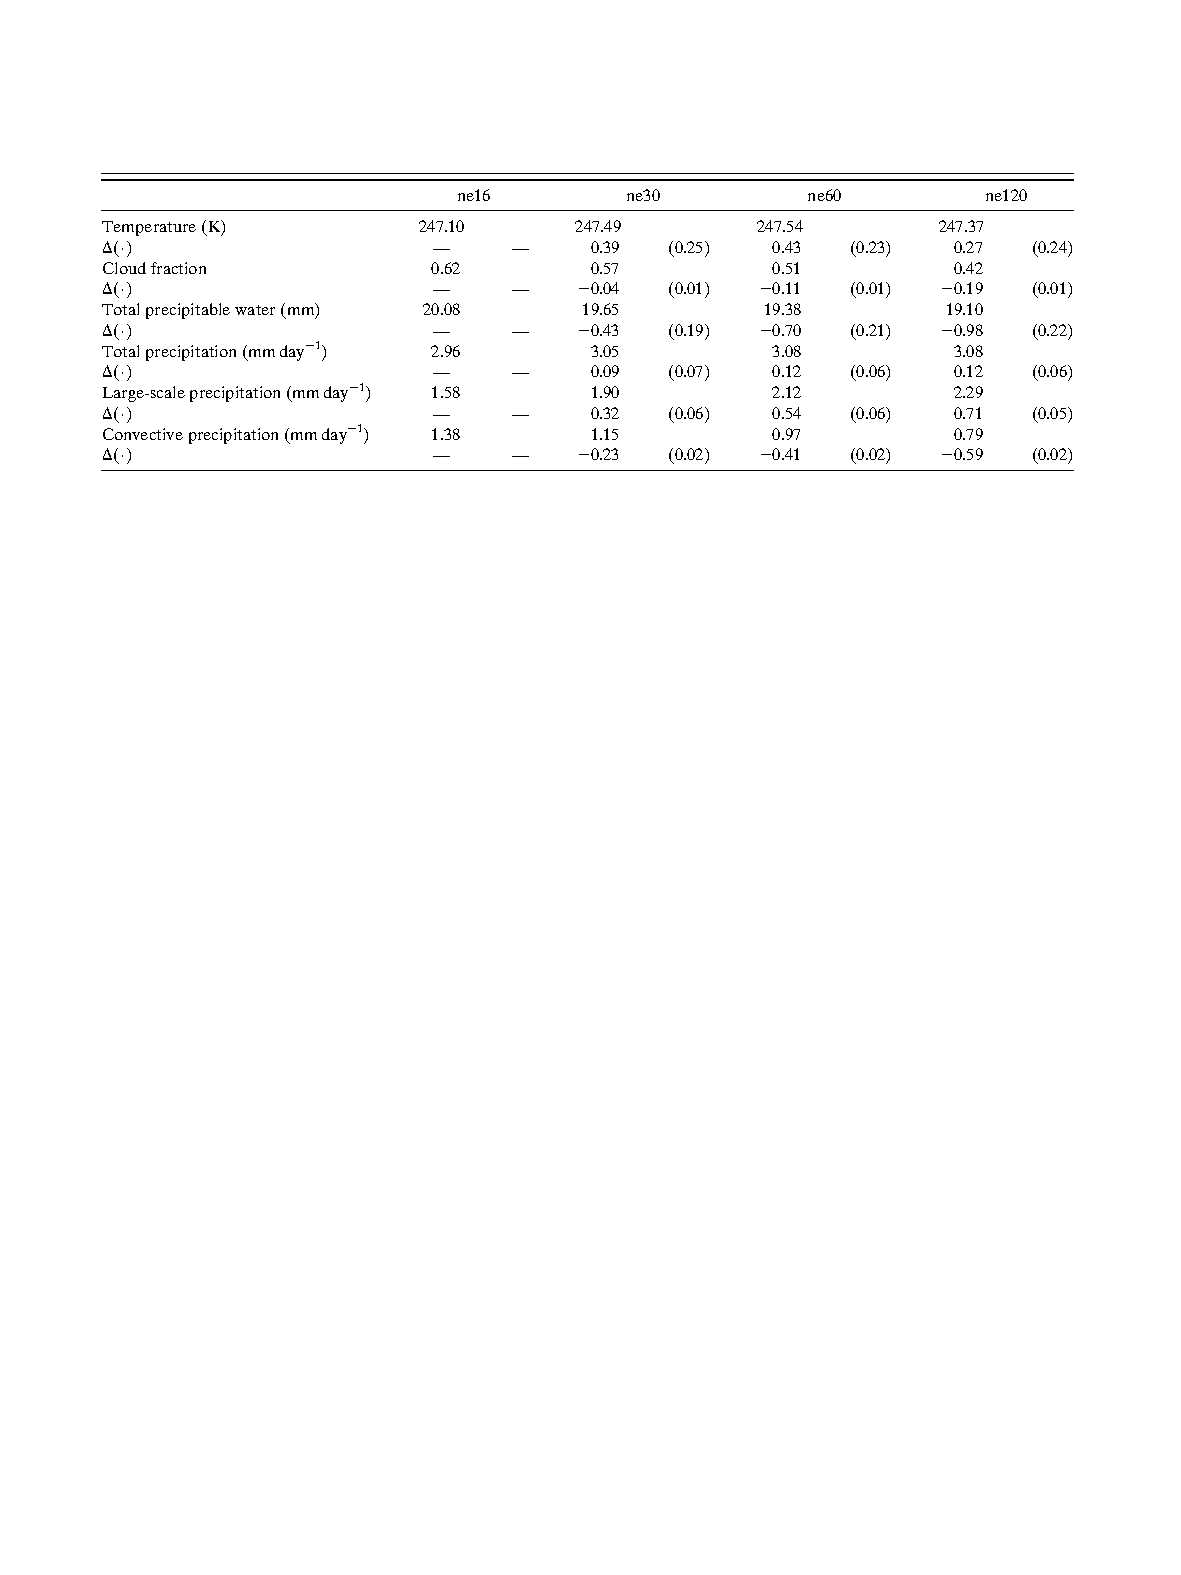
\includegraphics[width=30pc,angle=0]{chapter2/table1.pdf}\\
\end{center}
\caption{Time-mean global integrals in the simulations. Differences with respect to the ne16 simulation are indicated with a $\Delta ( \cdot )$ and the standard deviations of the monthly mean anomalies are given in parentheses.}
\label{tbl:table2-1}
\end{table}

Global temperatures are relatively invariant to resolution (Table~\ref{tbl:table2-1}), partially a reflection of the fixed sea surface temperatures in the aqua-planet configuration. The atmosphere becomes progressively drier with increasing resolution. Global mean total precipitable water is reduced by $0.98 \pm 0.22$ mm, about 5\% at the highest simulated resolution (ne120) relative to the control. The progressive drying trend is robust, since the anomalies in total precipitable water exceed two standard deviations (Table~\ref{tbl:table2-1}). Global average cloud fraction is also progressively reduced with increasing resolution (Table~\ref{tbl:table2-1}). The magnitude of the trend in cloud fraction is drastic, decreasing by approximately a third, or $0.19 \pm 0.01$ at the highest resolution relative to the control. The reduction in cloud fraction is split evenly between convective clouds and clouds associated with large-scale precipitation, at all resolutions (not shown). The high sensitivity of cloud fraction to resolution is well known in CAM4 \citep{OETAL2013JCLIM,RETAL2013JCLIM,ZetAl2014JCb} and earlier versions \citep{KW1991JGR,W2008TELLUS}, but there is little evidence for this sensitivity in the default physics package in CAM, version 5 \citep[CAM5;][]{ZetAl2014JCb}.

Global mean total precipitation increases slightly with resolution, but appears to converge to 3.08 mm/day at the two highest resolutions. Total precipitation is the sum of the convective precipitation and the large-scale precipitation. The trends in the two forms of precipitation with resolution are progressive, large and compensating (Table~\ref{tbl:table2-1}). The global mean large-scale precipitation (convective precipitation) increases (decreases) by $0.71 \pm 0.05$ mm/day ($0.59 \pm 0.02$ mm/day) in the highest resolution simulation. The increase (decrease) of the large-scale (convective) precipitation rate with increasing horizontal resolution has previously been documented in CAM5 \citep{ZetAl2014JCb}, CAM4 \citep{OETAL2013JCLIM,RETAL2013JCLIM,ZetAl2014JCb} and earlier versions \citep{WETAL1995CD,W2008TELLUS}.

Changes to the hydrologic cycle with resolution may be expected to affect the flows of energy determining the global atmospheric energy budget. Energy fluxes at the interface of the model with the surface, $f(\eta_{SFC})$ , and the top of the model, $f(\eta_{TOP})$, are provided by the model and used to compute global energy budgets for the surface and atmosphere. A generic flux, $f$, may be integrated around the domain of the model to compute the globally integrated energy tendency due to the divergence of the flux. We use the convention that positive values indicate a gain of energy to the system, and positive fluxes are directed upward.

The surface and top of atmosphere energy budget, based on standard equations \citep{PO1992}, are presented in Table~\ref{tbl:table2-2}. The large top of atmosphere energy imbalance is taken up almost entirely by the surface energy imbalance, corresponding to a net gain of energy to the surface on the order of 20 W/m2 in all the simulations (Table~\ref{tbl:table2-2}). The large sink of energy to the surface is a consequence of the fixed lower boundary condition, which prevents the surface fluxes from adjusting to bring the surface into an energy balance. The globally integrated total atmospheric energy tendency per unit area, $F_{TOT}$, has only a slight imbalance of about -1 W/m2 in all the simulations, which is roughly the same magnitude as the low frequency variability (Table~\ref{tbl:table2-2}) and together indicate the atmosphere is in a near balance on monthly timescales throughout the simulations. 

The global atmospheric energy budget per unit area may be expressed as,
\begin{eqnarray}
F_{TOT} = F_{CS} + F_{CD} + F_{S} + F_{SH} + L(P_L + P_C), \label{eq:eq2-2}
\end{eqnarray}
where the energy gain due to the divergence of the longwave radiative fluxes are separated into clear sky and cloud components ($F_{CS}$ and $F_{CD}$, respectively), such that their sum is the all-sky longwave term. Each of the longwave terms are related to the fluxes at the surface and top of atmosphere as $F = f(\eta_{SFC}) - f(\eta_{TOP})$. Note that $F_{S}$ is the gain in energy associated with atmospheric absorption of solar radiation, $F_{SH}$ is the surface sensible heat term and $L(P_L + P_C)$ is the surface latent heat term, expressed as the latent heat of condensation $L$ multiplied by the sum of the global mean large-scale precipitation rate $P_L$ and the global mean convective precipitation rate $P_C$, which are provided in Table~\ref{tbl:table2-1}.

\begin{table}[t]
\begin{center}
\noindent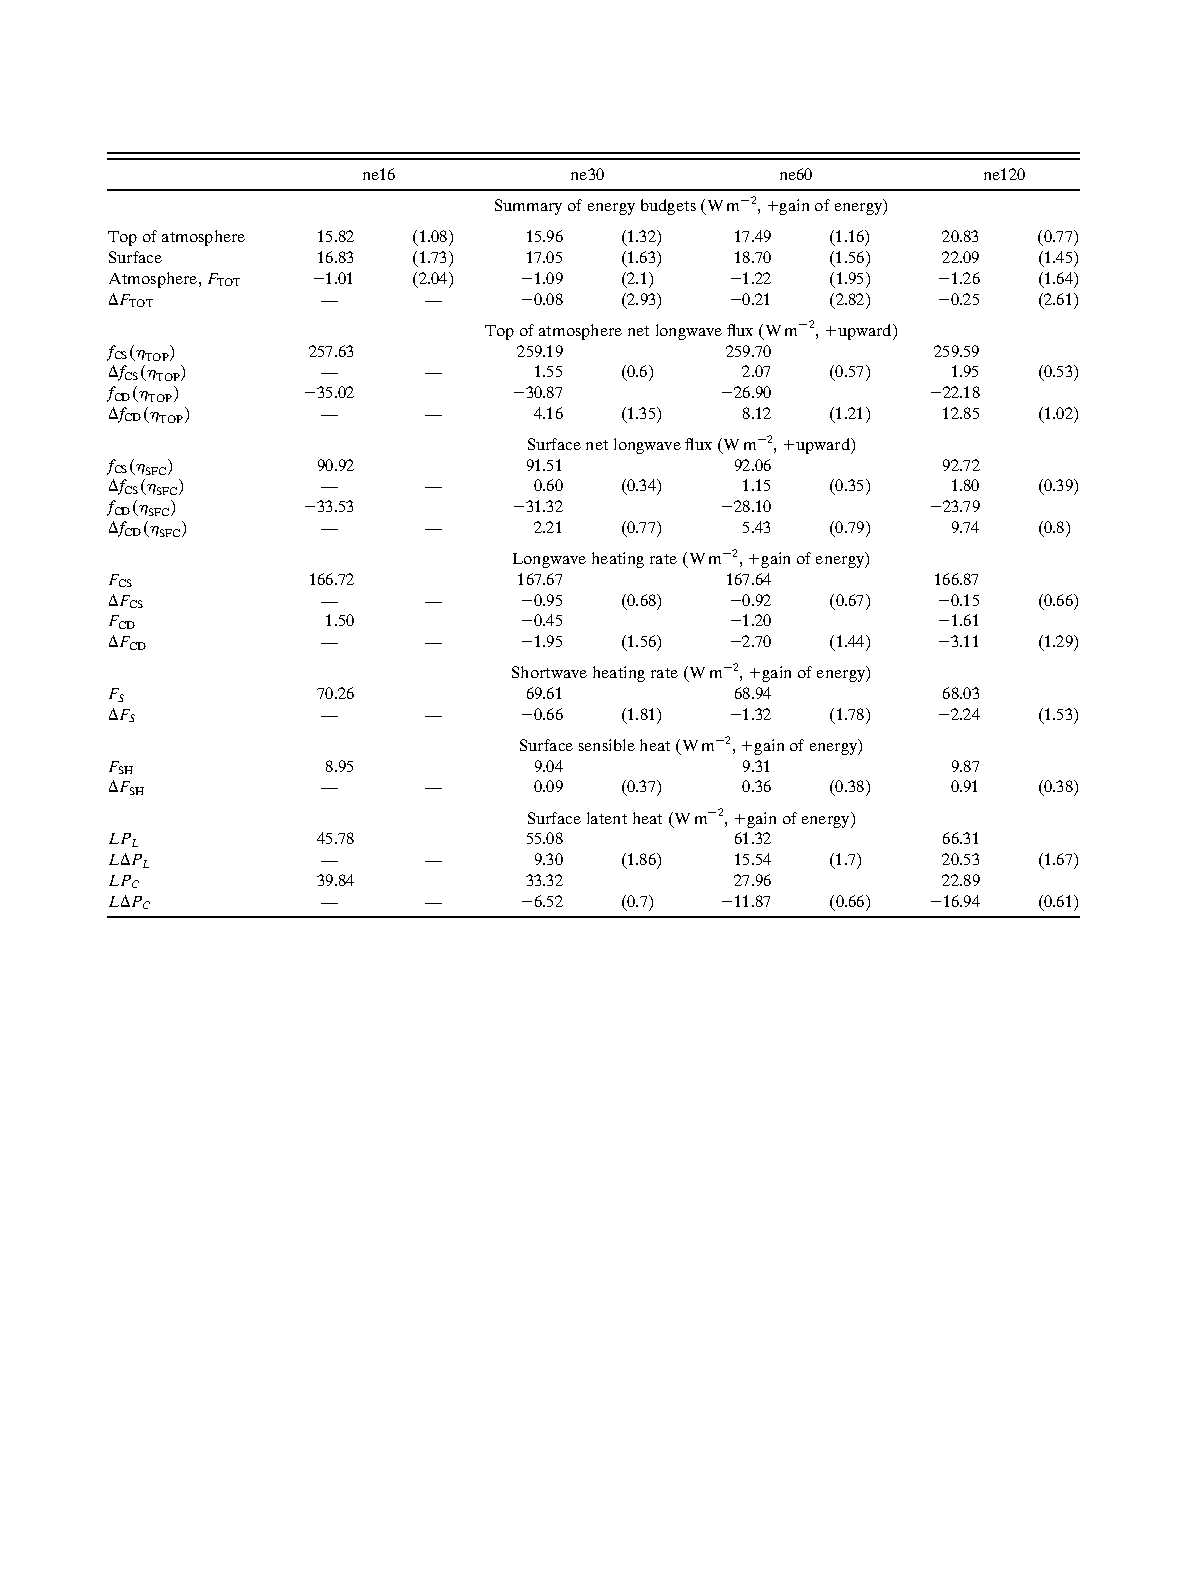
\includegraphics[width=30pc,angle=0]{chapter2/table2.pdf}\\
\end{center}
\caption{Global energy budgets in the simulations.}
\label{tbl:table2-2}
\end{table}

Clear-sky longwave radiative fluxes are on the order of 1-2 W/m2 higher than in the control simulation, and the trend is not monotonic with resolution. The clear-sky longwave fluxes at the surface are monotonic with resolution, increasing by up to $1.8 \pm 0.39$ W/m2 in the ne120 simulation. The trend in clear-sky surface fluxes indicate a reduction in downward longwave fluxes at the surface as they are sourced from higher and colder layers, consistent with increased atmospheric transmissivity in a drier atmosphere. The trends in clear sky fluxes at the top and bottom of the atmosphere compensate for one another, yielding a weak sensitivity of the clear sky longwave radiative heating rate to horizontal resolution (Table~\ref{tbl:table2-2}).

The longwave cloudy fluxes at the top of atmosphere increase monotonically with resolution by up to $12.85 \pm 1.02$ W/m2 in the ne120 simulation relative to the control. The large magnitude changes in longwave cloud fluxes are consistent with the large reduction in global cloud fraction in Table~\ref{tbl:table2-1}. At the surface, longwave fluxes due to clouds also progressively increase with resolution, but by a smaller amount than the top of atmosphere fluxes (Table~\ref{tbl:table2-2}). The surface and top of atmosphere fluxes combine to yield a longwave effect of clouds on the atmospheric energy budget that is two orders of magnitude less than the energy tendency associated with clear-sky longwave radiation. However, the magnitude of the change in the cloud forcing term with horizontal resolution is comparable to the trend in the clear-sky term, increasing progressively with resolution by up to $3.11 \pm 1.29$ W/m2 in the highest resolution simulation relative to the control.

The largest changes to the atmospheric energy budget with resolution occur within the latent heating term. The monotonic increase in latent heating associated with the trend in large-scale precipitation rate is large, up to a $20.53 \pm 1.67$ W/ m2 increase in the highest resolution simulation relative to the control (Table~\ref{tbl:table2-2}). These large magnitude changes to the atmospheric energy budget are mostly balanced by reductions in the global convective precipitation rate. Sensible heating is about an order of magnitude smaller than latent heating in the simulations, and are relatively insensitive to changes in resolution (Table~\ref{tbl:table2-2}). 

Atmospheric absorption of solar radiation decreases with resolution by $2.24 \pm 1.53$ W/m2 in the ne120 simulation relative to the control. Decreased shortwave absorption is due to greater transmissivity from a drier atmosphere, despite increased availability of shortwave radiation owing to large reductions in cloud fraction. 

\subsubsection{Regional Sensitivity}
An energy budget may be rewritten for zonal columns of energy with infitesimally thin meridional thickness. Expressed as a zonal average, the atmospheric energy budget differs from the global budget (equation~\ref{eq:eq2-2}) by a transport term \citep{PO1992}, 
\begin{eqnarray}
H(\phi) = \nabla \int \overline{\mathbf{V} s} + \frac{d}{dp} \int \overline{\omega s}, \label{eq:eq2-3}
\end{eqnarray}
where $H$ is the column integrated divergence of the flux of dry static energy, $s = c_p T + g Z$, for an infitesimally thin zonal slice at latitude $\phi$; $\mathbf{V} = (u,v)$  is the horizontal wind vector, $\omega$ is the vertical pressure velocity, $\nabla$ is the horizontal divergence operator and the terms $c_p$, $T$ and $Z$ are the specific heat capacity of dry air at constant pressure, air temperature and geopotential height, respectively. The integral refers to a mass weighted vertical integral over the atmospheric column in pressure coordinates ($\int = \int dp/g$) where $p$ is pressure. The overbar notation indicates a zonally and temporally averaged quantity.

\begin{figure}
\begin{center}
\noindent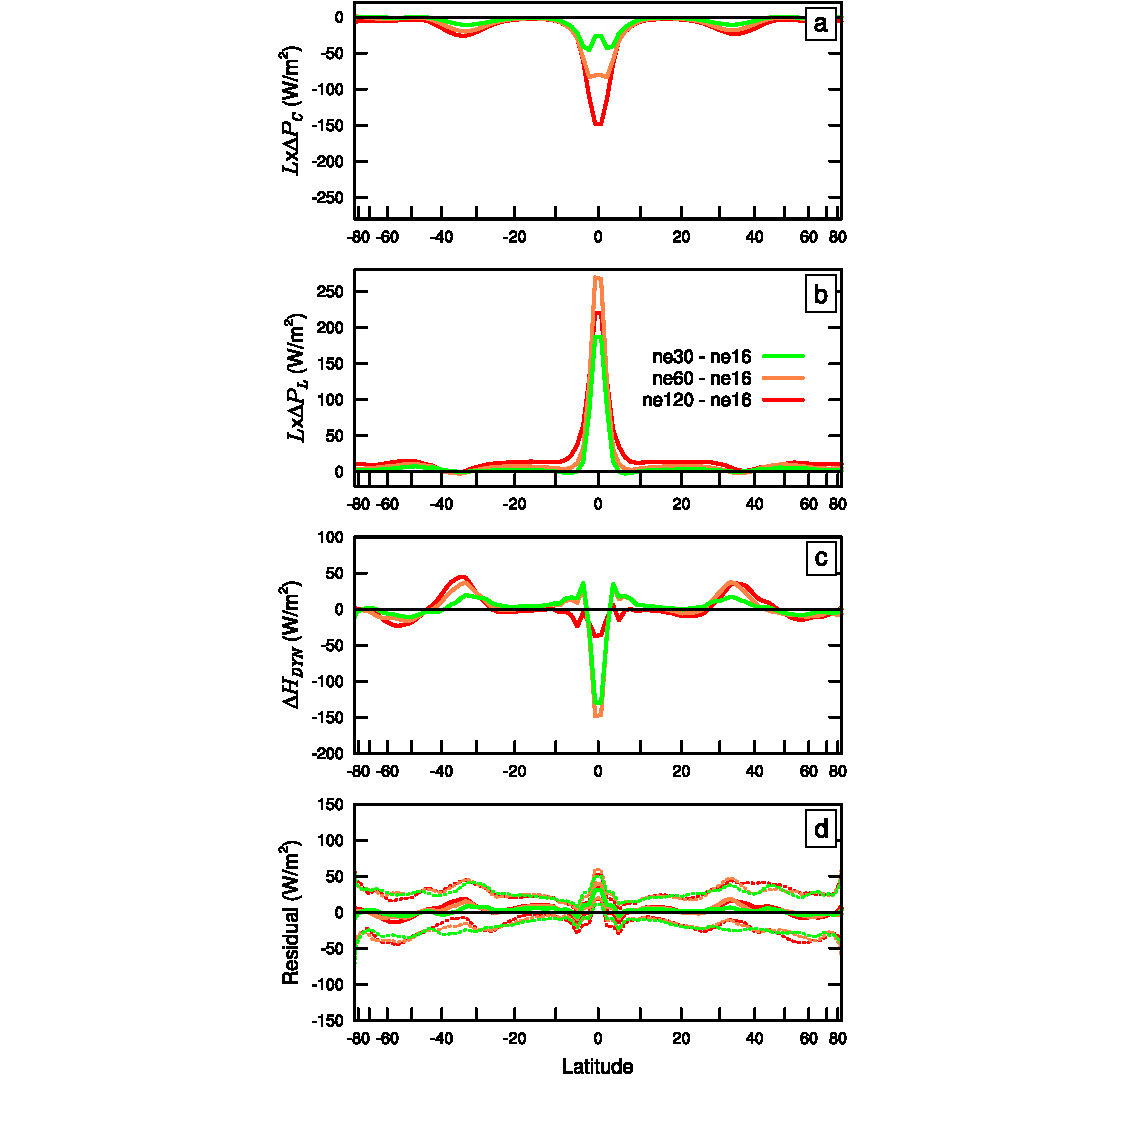
\includegraphics[width=20pc,angle=0]{chapter2/figure1.pdf}\\
\end{center}
\caption{Departure of the components of the zonal average energy budget from the ne16 simulation. Anomalies in latent heat associated with (a) convective precipitation and (b) large-scale precipitation, (c) the dynamical component of the anomalous divergence of the flux of dry static energy by the mean vertical circulation and (d) the residual computed from the sum of (a), (b) and (c). Dotted lines refer to twice the standard deviation associated with low frequency (monthly) variability.}
\label{fig:figure2-1}
\end{figure}

Through evaluating the response of CMIP3 models to global warming emission scenarios, \cite{MO2011NATUREC} have shown that regional changes to the zonal average energy budget are well approximated by the change in the column integrated divergence of the flux of $s$ by the mean vertical circulation, $\Delta H_m$. This term can be decomposed into dynamic, $\Delta H_{DYN}$, and thermodynamic components, $\Delta H_{THM}$, as,
\begin{eqnarray}
\Delta H_m = \Delta H_{DYN} + \Delta H_{THM} = \int \Delta (\overline{\omega}) \frac{d \overline{s}}{dp} + \int \overline{\omega} \Delta (\frac{d \overline{s}}{dp}), \label{eq:eq2-4}
\end{eqnarray}
Making the assumption $\Delta H  \sim \Delta H_m$, the change in the zonally averaged atmospheric energy budget between two simulations may be expressed as,
\begin{eqnarray}
\Delta F_{TOT} (\phi)= L[\Delta P_L (\phi) + \Delta P_C (\phi)] + F_{DC} (\phi) + \Delta H_{DYN} (\phi) + \Delta H_{THM} (\phi), \label{eq:eq2-5}
\end{eqnarray}
where $F_{DC} = F_S + F_{CL} + F_{CD} + F_{SH}$ contains the diabatic cooling terms. Figure~\ref{fig:figure2-1}a,b shows the zonal average latent heat anomalies associated with changes in convective and large-scale precipitation relative to the ne16 simulation. The overall reduction in convective precipitation manifests as a strong, monotonic reduction in latent heating with resolution at the equator, and to a lesser extent in the subtropics. The large-scale precipitation more than compensates for the relative loss of energy due to reductions in convective precipitation at the equator. The anomalous heating due to changes in large-scale precipitation in the ne120 simulation is intermediate to the ne30 and ne60 anomalies at the equator. While the maximum anomalies at the equator are not monotonic with resolution, the width of the equatorial anomaly does become progressively wider with resolution and there is a slight increase in heating with resolution almost everywhere outside the equator.

Figure~\ref{fig:figure2-1}c shows the dynamical component, $\Delta H_{DYN}$ of the divergence of the flux of $s$, due to the change in the mean vertical circulation. The value of $\Delta H_{DYN}$ becomes progressively more negative at the equator in the ne30 and ne60 simulations, and positive anomalies persist just outside the equator. In contrast, the ne120 simulation remains negative just outside the equator and the magnitude of the equatorial minimum in $\Delta H_{DYN}$ is less than in the ne30 or ne60 simulations. Near the subtropics $\Delta H_{DYN}$ becomes increasingly positive with resolution (Figure~\ref{fig:figure2-1}c), indicating enhanced subsidence. Anomalous heating from greater subsiding motion is primarily balanced by reductions in subtropical convective precipitation (Figure~\ref{fig:figure2-1}).

Qualitatively, the spatial distributions of latent heat anomalies are of a similar order of magnitude as $\Delta H_{DYN}$ and appear compensatory. Figure~\ref{fig:figure2-1}d shows the sum of the three terms $L(\Delta P_L + \Delta P_C) + \Delta H_{DYN}$, which may be interpreted as the latent heating anomalies that are not balanced by $\Delta H_{DYN}$. The sum of these three terms is generally small compared to the individual terms, suggestive of a first-order balance of the anomalous energy. 

The relative change in diabatic cooling, $\Delta F_{DC}$, although important in the global mean (Table~\ref{tbl:table2-2}), has very little influence on large regional changes to the energy budget observed in the simulations (not shown). This result is consistent with the response of CMIP3 models to global warming emissions scenarios (Muller an O’Gorman 2011). In contrast to \cite{MO2011NATUREC}, $\Delta H_{THM}$ is also small and shows minimal variation with latitude (not shown). The small contribution of $\Delta H_{THM}$ to the anomalous energy budget indicates that the distribution of $s$ in the simulations is not very sensitive to resolution, partially a reflection of the fixed sea surface temperatures in the aqua-planet configuration. The remaining heating anomalies in Figure~\ref{fig:figure2-1}d may be balanced by neglected transport terms or energy storage.

Interestingly, the residual heating appears to converge to a similar zonal distribution by ne30 (Figure~\ref{fig:figure2-1}d). While the source of this residual may be uncertain, it indicates that the sensitivity of the zonal average energy budget to resolution in the ne30, ne60 and ne120 simulations is contained within the latent heating and $\Delta H_{DYN}$ terms. As $\Delta H_{DYN}$ is proportional to the change in the resolved vertical motion, our results indicate that an active vertical velocity field is providing a balance to the large variations in latent heating observed in the model. \cite{YETAL2014JCLIM} come to a similar conclusion through analysis of the moisture budget for extreme precipitation events, which together indicate that important changes to the resolved vertical velocity field are common to the sensitivity of mean and extreme statistics with resolution.

\begin{figure}
\begin{center}
\noindent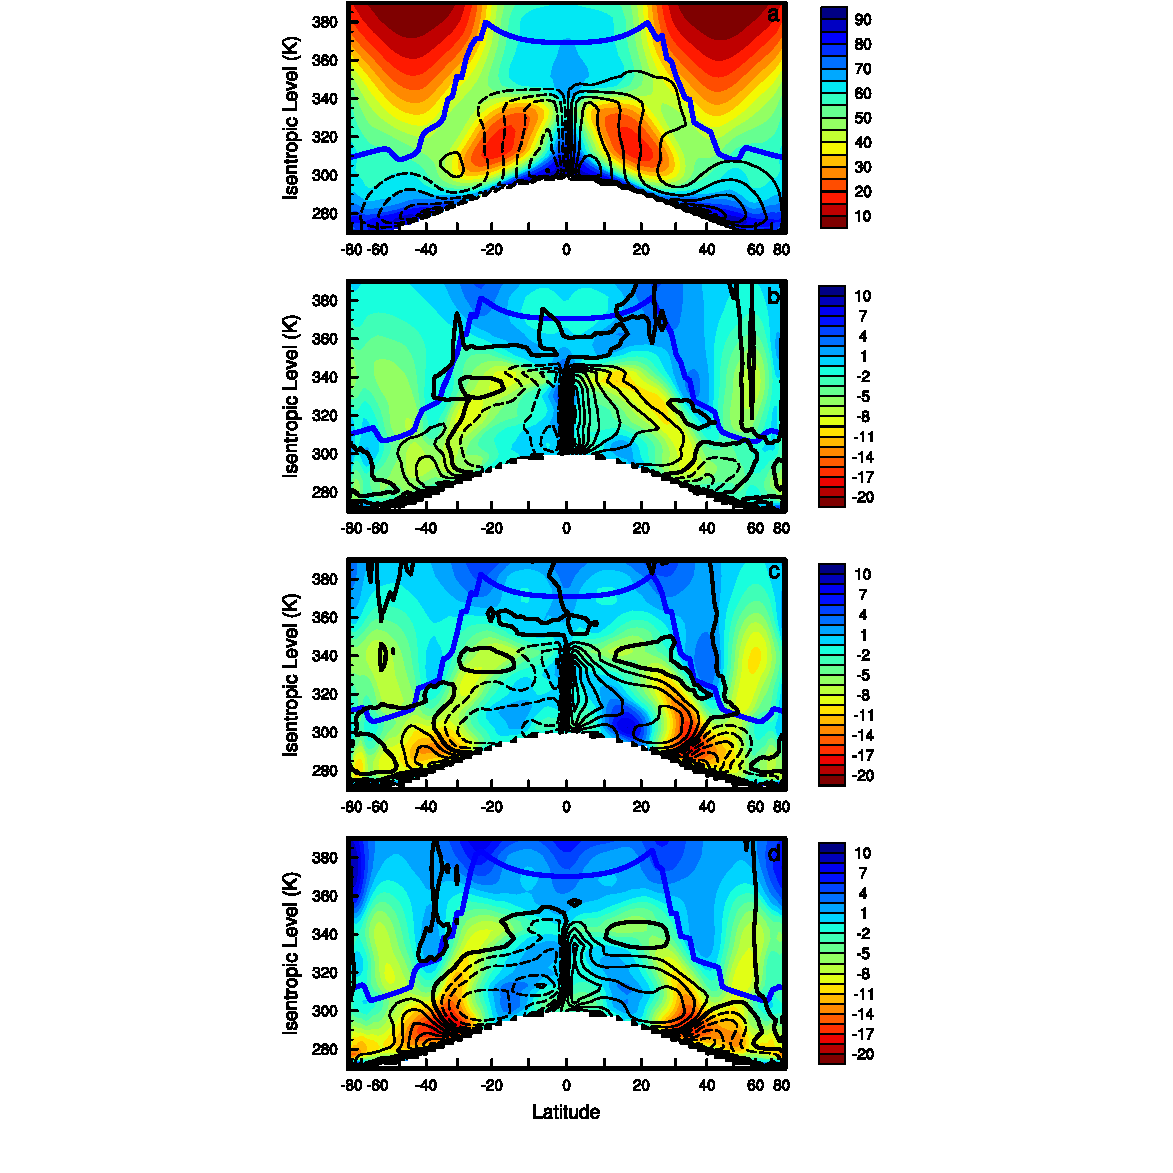
\includegraphics[width=20pc,angle=0]{chapter2/figure2.pdf}\\
\end{center}
\caption{(a) Zonally averaged isentropic meridional streamfunction (black lines) and relative humidity field (color) in the ne16 control. Contour interval is $50 \times 10^9$ kg/s. (b-d) Departures of the zonally averaged isentropic meridional streamfunction and relative humidity field from the ne16 control in the (b) ne30 (c) ne60 and (d) ne120 simulations. Contour interval is $10 \times 10^9$ kg/s. Solid (dashed) lines correspond to clockwise (counter-clockwise) motion and thick solid line corresponds to the zero contour. Blue solid line is the tropopause height computed using a lapse-rate WMO definition.}
\label{fig:figure2-2}
\end{figure}

Changes to the zonal-mean time-mean resolved upward motion near the equator, along with increases in subtropical subsidence, implies a change in the large-scale Hadley Circulation with resolution. Figure~\ref{fig:figure2-2}b-d shows the departure of the mean isentropic meridional mass streamfunction in the simulations from the mean in the control simulation (Figure~\ref{fig:figure2-2}a). At the equator, an anomalous overturning cell extending into the upper-troposphere occurs in the ne30 simulation (Figure~\ref{fig:figure2-2}b). The descending branch of the anomalous equatorial circulation is split between a local branch, confined to within $10^{\circ}$ of the equator, and a poleward traveling branch, flowing under subtropical jet core (not shown) and extending to about $40^{\circ}$ latitude (Figure~\ref{fig:figure2-2}b). The anomalous poleward branch is unique in the sense that the mean Hadley Cell only extends to the latitude of the subtropical jet (Figure~\ref{fig:figure2-2}a), which remains in a fixed location in the simulations \citep{LETAL2015JCLIM}. At higher resolutions, the local descending branch becomes weaker and more confined in the meridional direction, while the poleward branch becomes more pronounced, merging with anomalous upward motion around $20^{\circ}$ to form a partially closed anomalous circulation extending to $40^{\circ}$ latitude (Figures~\ref{fig:figure2-2}c,d). The anomalous ascent near $20^{\circ}$ is consistent with the anomalous off equatorial heating in Figure~\ref{fig:figure2-1}b. While generally the Hadley Cell tends to intensify with resolution, the spatial complexities of the anomalies indicate that changes in the Hadley Cell are not a simple uniform increase in intensity of the mean overturning cell depicted in Figure~\ref{fig:figure2-2}a.

\subsubsection{Moisture Budget}
Changes in the distribution and strength of resolved mass transport in the atmosphere have profound impacts on the distribution of water vapor, which directly influences the cloud amount diagnosed by CAM. Figure~\ref{fig:figure2-2}b-d shows variations in zonal mean relative humidity relative to the ne16 simulation (Figure~\ref{fig:figure2-2}a). Despite increases in relative humidity in and above the upper-troposphere, and within the subtropical dry zone, there is a clear tendency towards a drier atmosphere with resolution. The reduction in global average cloud fraction with resolution (Table~\ref{tbl:table2-1}) is directly related to the reductions in relative humidity, since the macrophysics scheme computes the cloud fraction as a simple function of the relative humidity field in CAM4 \citep{CAM4,PETAL2014JCLIM}. The greatest reduction in clouds occurs at the overlap between where clouds are abundant and regions that experience the greatest amount of drying (not shown).

The most pronounced changes in moisture in the simulations are the progressive reductions in subtropical relative humidity with resolution in the region of elevated subsidence identified in Figure~\ref{fig:figure2-1}c. The maximum reduction in relative humidity occurs in the ne120 simulation, decreasing by a third or 20\% at the 290 K level in the vicinity of $30^{\circ}$ latitude and leading to the complete elimination of clouds in this region (not shown). The drying anomalies are aligned with the anomalous poleward branch, which descends into the region of maximum drying (Figures~\ref{fig:figure2-2}b-d). Drying anomalies also coincide with an anomalous extra-tropical circulation, aligned with an equator-ward subsiding branch that becomes stronger with increasing resolution (Figure~\ref{fig:figure2-2}b-d).

To unravel the role of different processes influencing the relative humidity changes, Figure~\ref{fig:figure2-3} shows some components of the time-mean zonal averaged moisture budget in isentropic coordinates after \cite{SETAL2006JCLIM}, for the northern hemisphere only. The isentropic moisture budget naturally separates along and cross-isentropic mixing, which approximate different mechanisms controlling the relative humidity of the atmosphere \citep{SETAL2006JCLIM}. The descending branch of the Hadley Cell is a cross-isentropic process that exports dry air from upper levels to lower levels of the troposphere \citep{P1999GM}. The moisture budget of the subtropics is also influenced by extra-tropical recirculation, which is an approximately adiabatic process \citep{GETAL2005JAS,SETAL2006JCLIM}. Extra-tropical recirculation refers to moisture advected out of the subtropics, condensing along poleward trajectories and re-circulating back into the subtropics \citep{GETAL2005JAS}.

The zonal averaged moisture balance in isentropic coordinates is \citep{SETAL2006JCLIM},
\begin{eqnarray}
\partial_t (\overline{\rho_{\theta}} \, \overline{q}^{\ast}) + \partial_y (\overline{\rho_{\theta}} \, \overline{v}^{\ast} \, \overline{q}^{\ast}) + \partial_{\theta} (\overline{\rho_{\theta}} \overline{Q}^{\ast} \overline{q}^{\ast}) + \partial_y (\overline{\rho_{\theta}} \, \overline{v^{\prime} q^{\prime}}) + \partial_{\theta} (\overline{\rho_{\theta}} \, \overline{Q^{\prime} q^{\prime}}) = \overline{\rho_{\theta}} \overline{S}^{\ast}, \label{eq:eq2-6}
\end{eqnarray}
where $q$ is the specific humidity, $S = \frac{dq}{dt}$ and $Q = \frac{d \theta}{dt}$ are the specific humidity and diabatic forcing terms from the column physics. Primes denote fluctuations about the zonal and temporally averaged mean. The zonal average moisture tendency in isentropic coordinates reflects a balance between moisture sources, $\overline{\rho_{\theta}} \overline{S}^{\ast}$, and the divergence of mean and eddy fluxes of moisture along and across isentropic surfaces.

\begin{figure}
\begin{center}
\noindent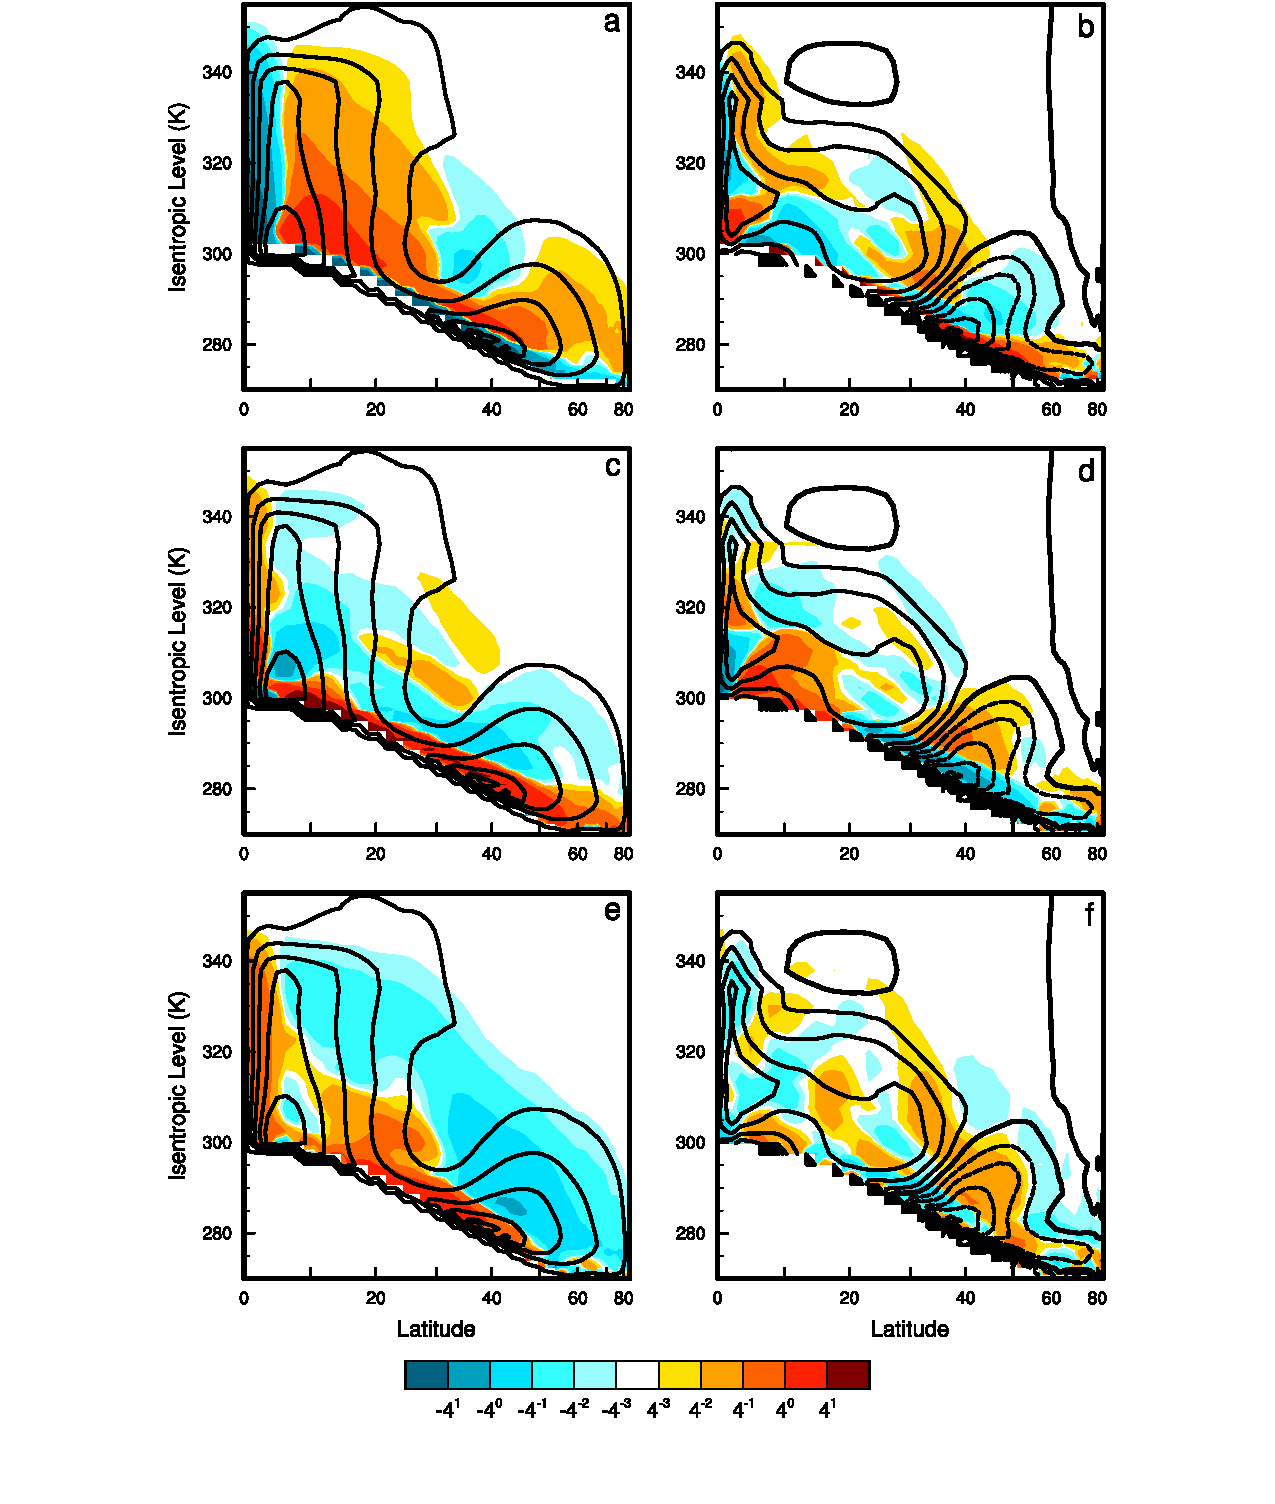
\includegraphics[width=30pc,angle=0]{chapter2/figure3.pdf}\\
\end{center}
\caption{(a), (c) and (e) Components of the zonal average moisture budget in isentropic coordinates in the ne30 simulation. (b), (d) and (e) Departure of the components of the zonally averaged moisture budget in the ne120 simulation from the ne16 control. (a), (b) Divergence of the cross isentropic moisture transport by the mean, (c), (d) divergence of the along isentropic moisture transport by the mean and (e), (f) divergence of the along isentropic eddy transport. Units are in $10^{-6}$ kg/m2/K/s and the meridional streamfunction contours are as in Figure~\ref{fig:figure2-2}.}
\label{fig:figure2-3}
\end{figure}

Figure~\ref{fig:figure2-3}b,d,f show the departure of the mean cross-isentrope, $\partial_{\theta} (\overline{\rho_{\theta}} \overline{Q}^{\ast} \overline{q}^{\ast})$, mean along-isentrope, $\partial_y (\overline{\rho_{\theta}} \, \overline{v}^{\ast} \, \overline{q}^{\ast})$, and eddy along-isentrope, $\partial_y (\overline{\rho_{\theta}} \, \overline{v^{\prime} q^{\prime}})$, terms in the ne120 simulation relative to the ne16 simulation values, given in Figure~\ref{fig:figure2-3}a,c,e. The remaining terms of moisture budget could not be computed directly from the available model output. Anomalies in the mean cross-isentropic flux of moisture near the equator are characterized by low-level divergence and convergence aloft (Figure~\ref{fig:figure2-3}b). This pattern indicates extraction of moisture from the lower troposphere into the middle troposphere due to greater equatorial ascent. Anomalies in along-isentropic fluxes (Figure~\ref{fig:figure2-3}d,f) supply the lower troposphere with moisture at the equator, maintaining the cross-isentropic anomalies.

The large subtropical drying anomaly near $40^{\circ}$ (Figure~\ref{fig:figure2-2}d) is supported by anomalous divergence from all terms shown in Figure~\ref{fig:figure2-3}. The reduction in convective precipitation near $40^{\circ}$ opposes drying through relative increases in moisture source (not shown). The divergence of along isentropic eddy fluxes (Figure~\ref{fig:figure2-3}c) is most closely aligned with the drying anomaly flanking the anomalous poleward flow and extending into the region of maximum drying near $40^{\circ}$ (Figure~\ref{fig:figure2-2}d). This result is suggestive of greater eddy activity along the anomalous poleward flow. Figure~\ref{fig:figure2-4} shows the changes in the eddy momentum fluxes, $\overline{u^{\prime} v^{\prime}}$, with resolution, relative to the eddy fluxes in the ne16 simulation (Figure~\ref{fig:figure2-4}a). An increase in eddy activity lies just above the anomalous poleward flow, and the magnitude of the anomalous eddy fluxes increase with resolution (Figure~\ref{fig:figure2-4}). Alignment of the anomalous poleward flow with the anomalous eddy fluxes is suggestive of a momentum balance between the Coriolis force and the divergence of the eddy fluxes. Alternatively, the increased wave activity may be related to a reduction in effective dissipation of potential vorticity with resolution \citep{LETAL2015JCLIM}. 

\begin{figure}
\begin{center}
\noindent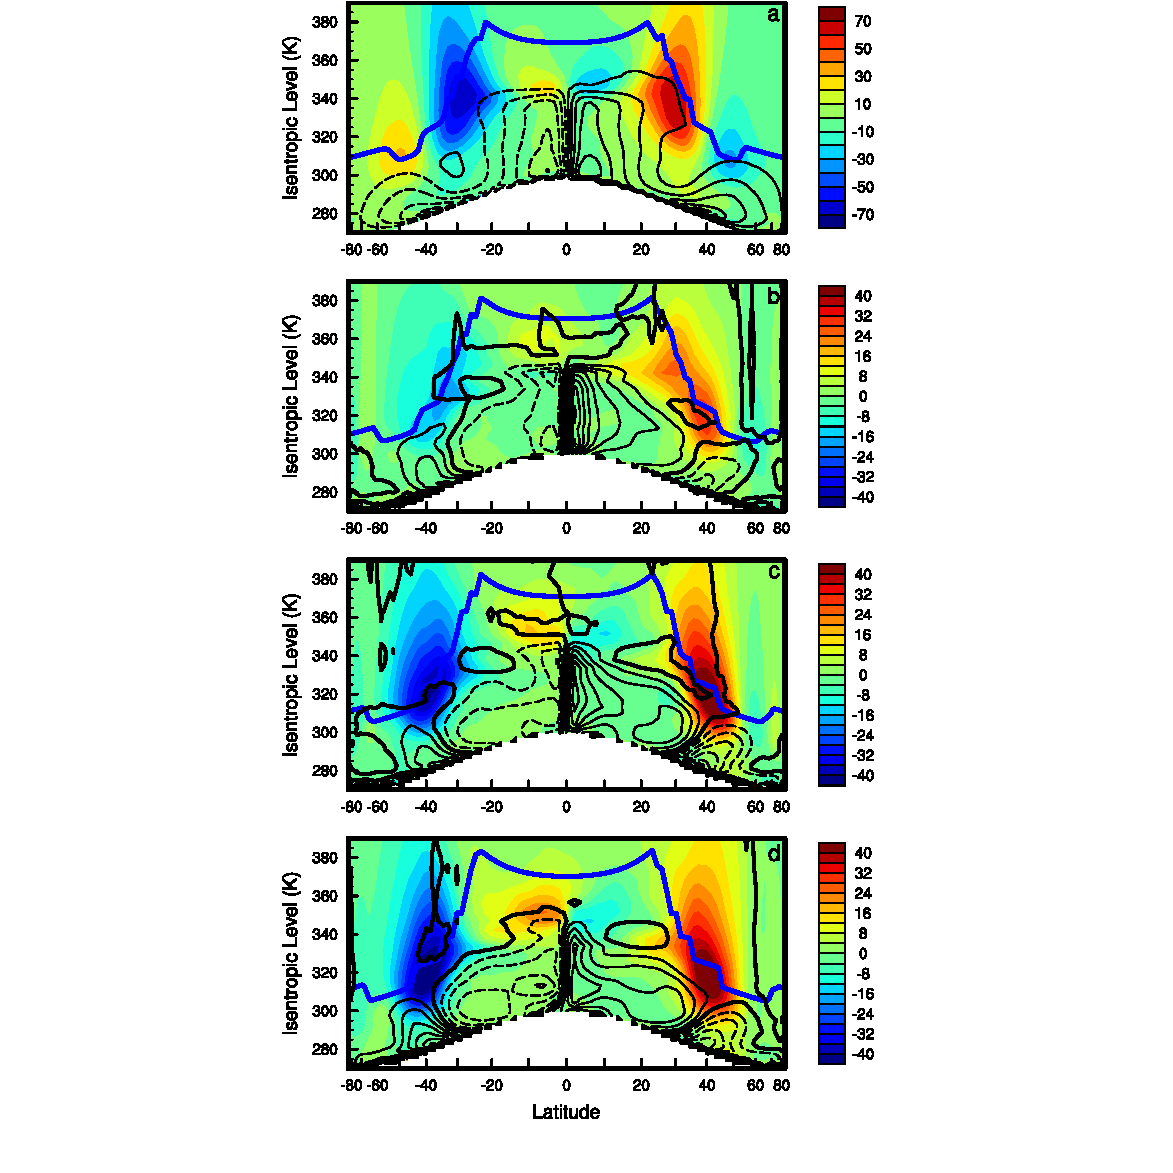
\includegraphics[width=20pc,angle=0]{chapter2/figure4.pdf}\\
\end{center}
\caption{As in Figure~\ref{fig:figure2-2}, but for the eddy fluxes $\overline{u^{\prime} v^{\prime}}$ in units of m2/s2.}
\label{fig:figure2-4}
\end{figure}

The large changes in cloud fraction (Table~\ref{tbl:table2-1}) are balanced by greater overturning of the Hadley Cell, greater isentropic mixing associated with variations in the extra-tropical circulation and a reduction in activity of the convection scheme. While this is not a particularly new finding \citep{KW1991JGR}, it indicates that the same underlying sensitivity of cloud coverage to resolution has continued to persist within the CAM lineage for at least 25 years.

\subsection{An Explanation}
Our results have demonstrated that a progressive drying of the atmosphere with increasing resolution is balanced through tropical and extra-tropical changes to the large-scale circulation. Here, we make the important simplification that many of the complexities embedded in the sensitivity of the large-scale circulation to horizontal resolution is a non-linear response to a resolution sensitive process rooted in linear Boussinesq theory. This simplification is unverified - its purpose is to provide the simplest possible interpretation of the resolution signal that is consistent with linear theory. We recognize that there may be other important resolution sensitive processes \citep[e.g.,][]{LETAL2015JCLIM}, but suggest that they are not sufficient to explain the large changes to the hydrologic cycle identified in the simulations. 

We begin with a non-hydrostatic, dry, non-rotating, frictionless atmosphere with no heat sources, a framework often used in the analysis of internal gravity waves \citep{H2004}. While the neglect of moist processes is clearly invalid for a moist GCM, the simplified framework may be viewed as approximating the evolution of individual dynamics time-steps in response to buoyant perturbations passed from the column physics. For solutions to a linearized vertical velocity perturbation of the type $w = w_0 exp[i(kx + mz + \sigma t)]$ in an unstable atmosphere, let $X^2 = -| N^2 |$, where $N^2$ is the buoyancy frequency. The dispersion relation is, 
\begin{eqnarray}
\sigma^2 = X^2 \frac{k^2}{k^2 + m^2},\label{eq:eq2-7}
\end{eqnarray}
where $\sigma$ is the unstable growth rate, $k$ is the horizontal wavenumber and $m$, the vertical wavenumber. According to equation~\ref{eq:eq2-7}, the growth rate is bounded by $X$ since $k/\sqrt{k^2 + m^2}$ is bounded by unity. That is, convergence occurs as the horizontal scale of motion is reduced from the hydrostatic limit ($k \ll m$), to within the non-hydrostatic limit ($k \approx m$). For deep tropospheric perturbations, the non-hydrostatic limit occurs at horizontal resolutions approaching the depth of the troposphere.

At hydrostatic scales ($k \ll m$), the unstable growth rate is approximately linear in $k$ (equation~\ref{eq:eq2-7}). The significance of $k$ in the numerator of equation~\ref{eq:eq2-7} can be traced back to the horizontal scale of the locally balanced hydrostatic pressure perturbation \citep{JR2016QJRMS}, driving horizontal convergence into the unstable air column and vertical motion. A model that permits removal of convective instability by the resolved dynamics results in an unstable growth rate, $\sigma$, that is linear in $k$ at hydrostatic scales. This result is true of both hydrostatic and non-hydrostatic models. The equivalent dispersion relation for hydrostatic models is $\sigma^2 = X^2 (k^2 / m^2)$, implying that hydrostatic solutions are unbounded in scale in the non-hydrostatic regime \citep{O1981JAS}, referred to as an ``ultra-violet catastrophe." This ultra-violet catastrophe is not relevant at typical truncation scales of present day GCMs. 

We hypothesize that the horizontal scale of the diabatic forcing from the column physics is proportional to the grid spacing, decreasing the horizontal scale of the hydrostatic pressure perturbations and increasing the unstable growth rate $\sigma$ and resolved vertical motion as the resolution is increased. A reduction in horizontal scale of the diabatic forcing arising from the column physics was identified in CAM by \cite{HETAL2006JCLIM}. Our hypothesis was motivated in part by the study of \cite{W1999T}, where convergence of the Hadley Cell was recovered in a prior version of CAM through fixing the horizontal scale of the physics forcing and increasing the resolution of the dynamical core. Our hypothesis attempts to explain the sensitivity of the resolved vertical motion in CAM with resolution identified in this study, and others \citep{KW1991JGR,LETAL2011TELLUS,YETAL2014JCLIM,OETAL2016JAMES}.

\begin{table}[t]
\begin{center}
\noindent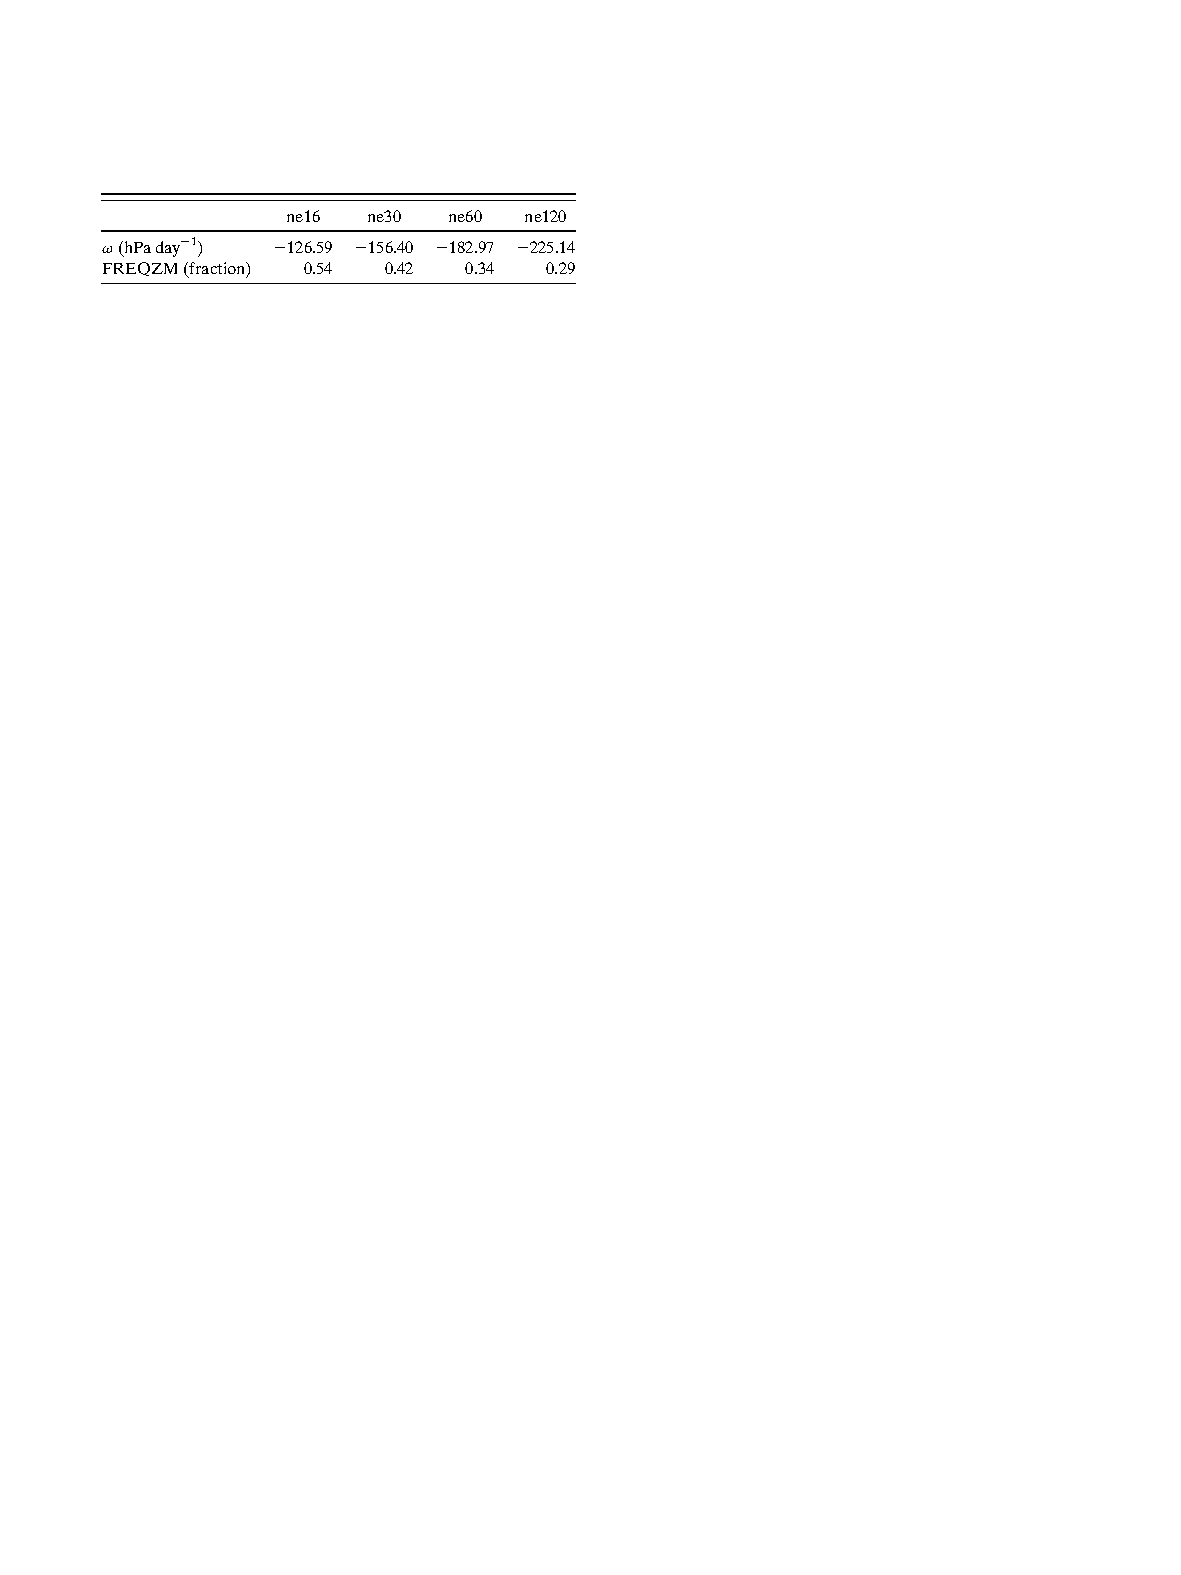
\includegraphics[width=20pc,angle=0]{chapter2/table3.pdf}\\
\end{center}
\caption{Mean upward vertical pressure velocity at 600 hPa and the fraction of time the deep convection scheme is active in the simulations (FREQZM) in the region $10^{\circ}$ N to $10^{\circ}$ S. }
\label{tbl:table2-3}
\end{table}

Mean values of the vertical pressure velocity at the 600 hPa level, conditionally sampled for upward motion in the ascent region of the Hadley Cell ($10^{\circ}$ N to $10^{\circ}$ S) are shown in Table~\ref{tbl:table2-3}. No interpolation was performed during this calculation and all values were computed on their native grids. Ascent velocities associated with the Hadley Cell increase with resolution, and show no indication of convergence. 

We argue that the increases in mean vertical velocities in Table~\ref{tbl:table2-3} are due to contributions of increasingly finer scales with increasing horizontal resolution. Figure~\ref{fig:figure2-5} shows the power spectra of 600 hPa vertical pressure velocities over the entire domain in the simulations, including upward and downward motion. Wavenumbers on the order 10 or less appear converged, potentially reflecting the ability of the model to resolve the deformation radius in all simulations and enabling realistic interactions between mid-latitude eddies and the mean flow \citep{W1999T,DV2000JCLIM,ZGETAL2015JAMES}. For wavenumbers on the order of 10 or larger, the general trend is for reduced power at lower wavenumbers and increased power at higher wavenumbers with increasing resolution (Figure~\ref{fig:figure2-5}). 

Snapshots of the vertical pressure velocities at the equator for the four different resolutions (Figure~\ref{fig:figure2-6}) provide further evidence that a transfer of variance to finer scales contributes to the observed variations in the mean state (Table~\ref{tbl:table2-3}). Resolved convective updrafts populate the equator, and their horizontal scale decreases with increasing resolution. This transfer of velocity variance to finer scales is consistent with the model results and emergent scaling presented by \cite{RETAL2016CD}, as well as linear Boussinesq theory (equation~\ref{eq:eq2-7}).

\begin{figure}[t]
\begin{center}
\noindent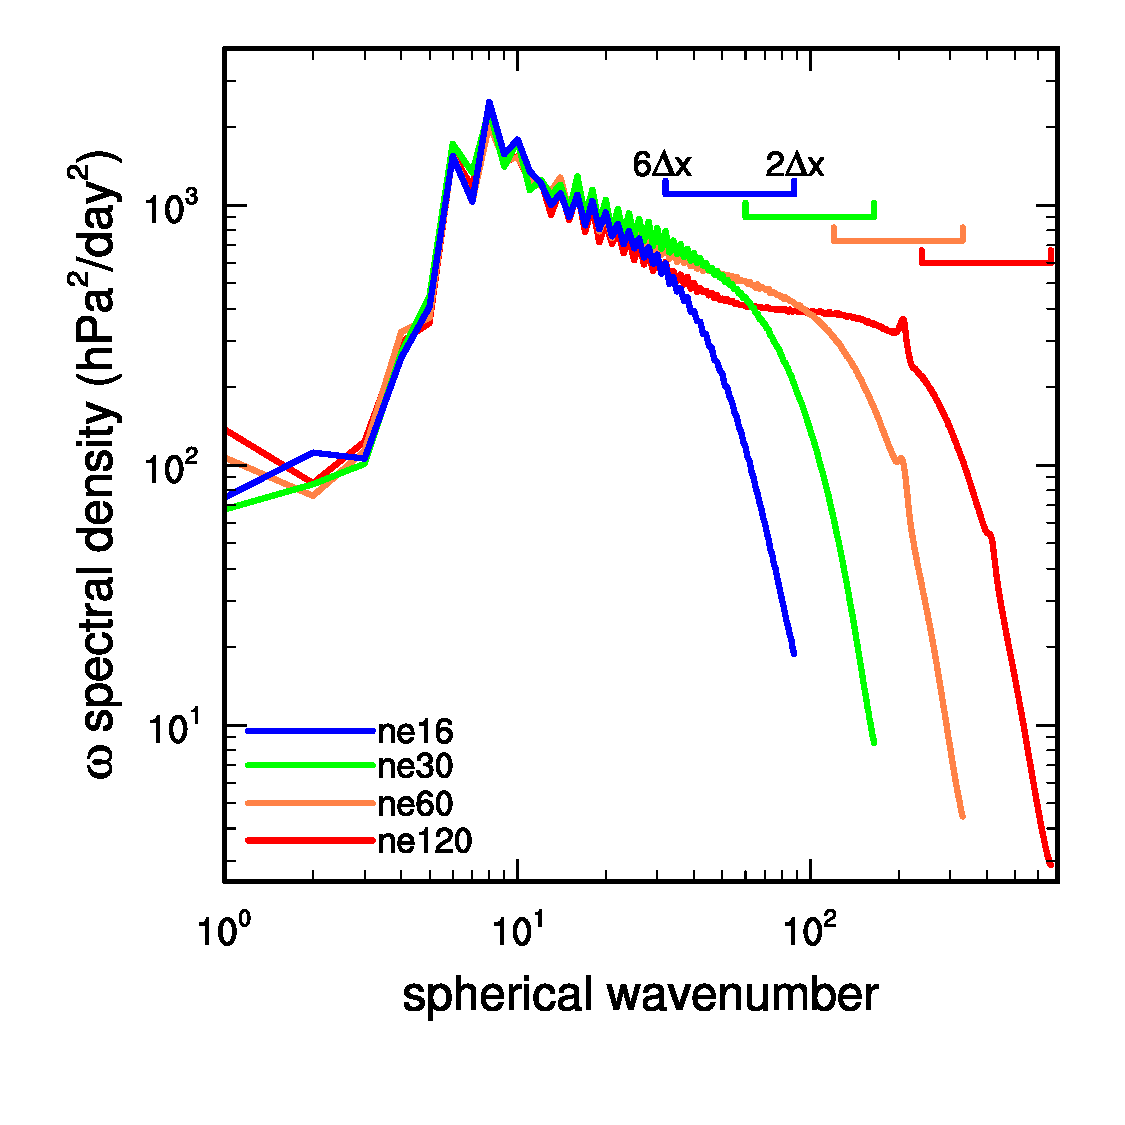
\includegraphics[width=20pc,angle=0]{chapter2/figure5.pdf}\\
\end{center}
\caption{Power spectral density of the 600 hPa vertical pressure velocity over the entire model domain. Values computed from 360 instances of 6-hourly output randomly selected from the integration period.}
\label{fig:figure2-5}
\end{figure}

\begin{figure}
\begin{center}
\noindent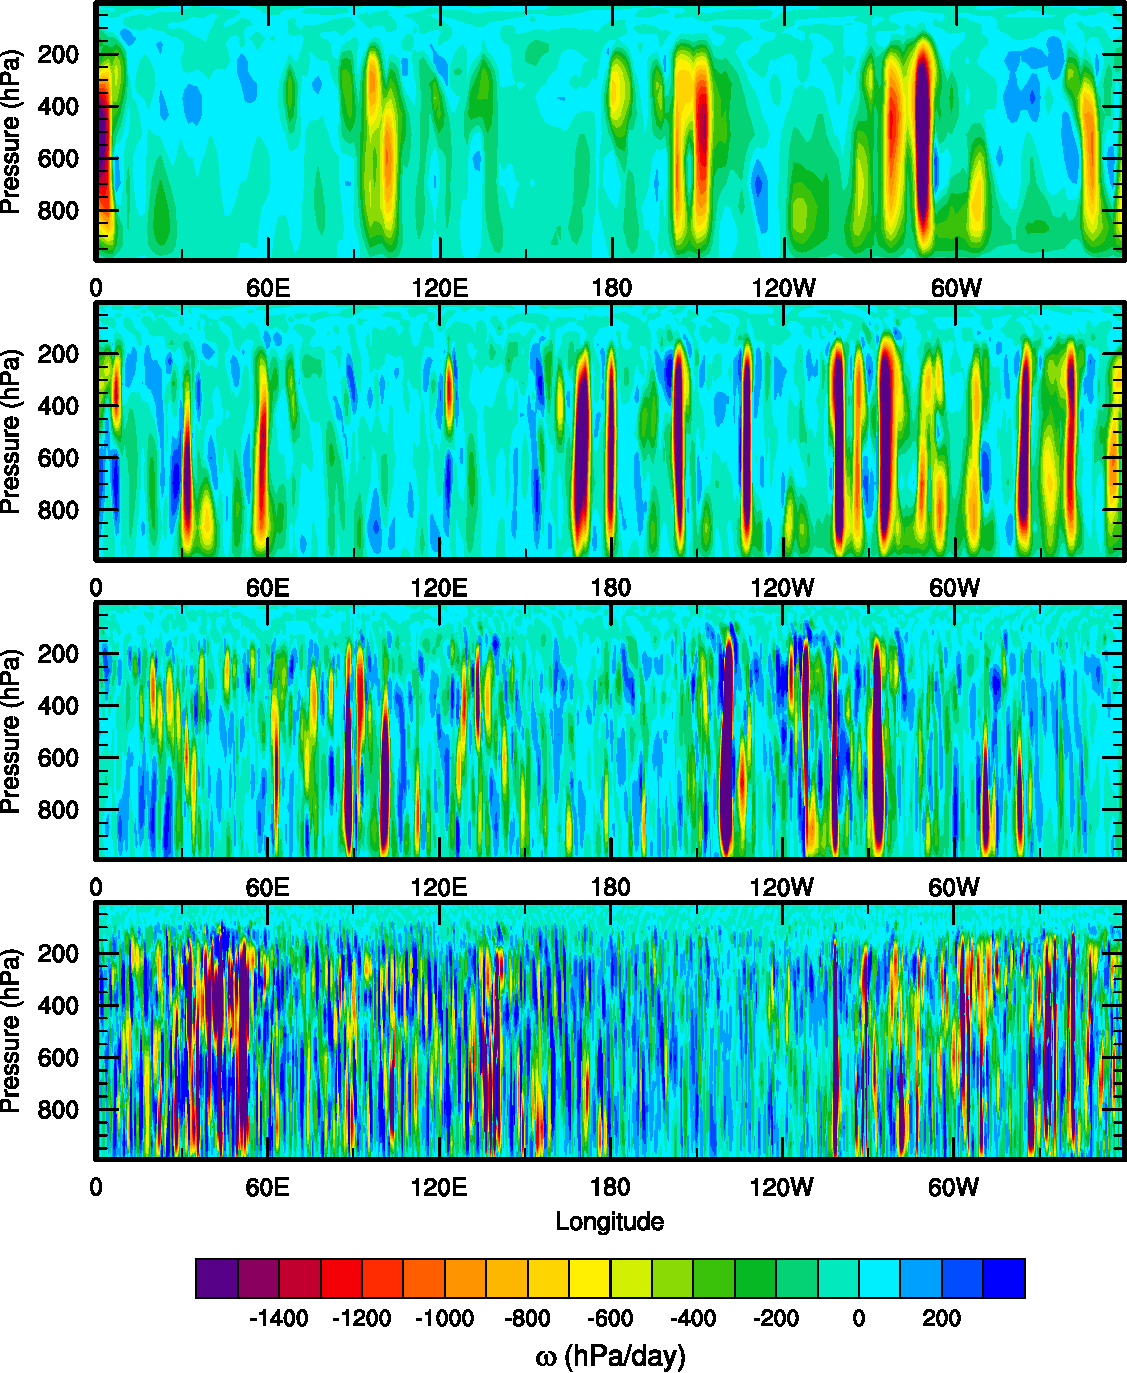
\includegraphics[width=35pc,angle=0]{chapter2/figure6.pdf}\\
\end{center}
\caption{Longitude-height instantaneous snapshot of the vertical pressure velocity at the equator during a randomly chosen time in the (a) ne16 (b) ne30 (c) ne60 and (d) ne120 simulations.}
\label{fig:figure2-6}
\end{figure}

The linear theory, and our hypothesis in general, is only applicable to convectively unstable conditions within the dynamical core. The occurrence of convectively unstable conditions may be thought to be infrequent in GCMs, as the convection schemes are designed to prevent the occurrence of resolved convection. Figure~\ref{fig:figure2-6}, however, provides evidence that resolved convection is a common occurrence in the deep tropics in CAM. Here, we propose an explanation for the occurrence of resolved convection in the presence of a convection scheme in CAM. The relevant ordering of the sub-models in our simulations, on the level of an individual physics time-step is the convection schemes, the large-scale precipitation scheme and the dynamics, respectively \citep{CAM4}. This process ordering implies that convectively unstable air produced by the large-scale condensation scheme interacts directly with the dynamics before the convection schemes are able to consume the instability. The resolved dynamics consume buoyancy at a rate proportional to $\omega$ in the thermodynamic equation, whose dynamics are approximated by the dispersion relation (equation~\ref{eq:eq2-7}). As the horizontal resolution of the model increases, resolved updrafts intensify with resolution, consuming buoyancy at an increasing rate. The convection scheme is then left with a smaller proportion of the available potential energy initially produced through the large-scale precipitation scheme. A caveat to this explanation is that the mean state is determined by the solution trajectory spanning many time-steps, which may not be reflective of processes occurring in a single time-step.

The activity of the deep convection scheme in the model is tied to an estimate of the available potential energy using a dilute plume calculation after \cite{RB1992JAS}. Although this quantity departs from the usual definition of the convective available potential energy (CAPE), we will refer to this quantity as CAPE throughout the discussion to be consistent with prior CAM studies. When CAPE exceeds 70 J/kg, the deep convection scheme is triggered (Neale et al. 2010). Unfortunately, CAPE is not available from the model output and we do not attempt to diagnose it from the available fields. A related quantity, the fraction of time in which the deep convection scheme is active in the simulations (FREQZM), is available from the model output and the mean values for the deep tropics are provided in Table~\ref{tbl:table2-3}. FREQZM is systematically reduced as the vertical velocities increase with resolution. We speculate that the resolved vertical motion becomes more effective at consuming available potential energy with increasing resolution, thereby reducing the frequency in which CAPE reaches its threshold value of 70 J/kg.

\begin{figure}
\begin{center}
\noindent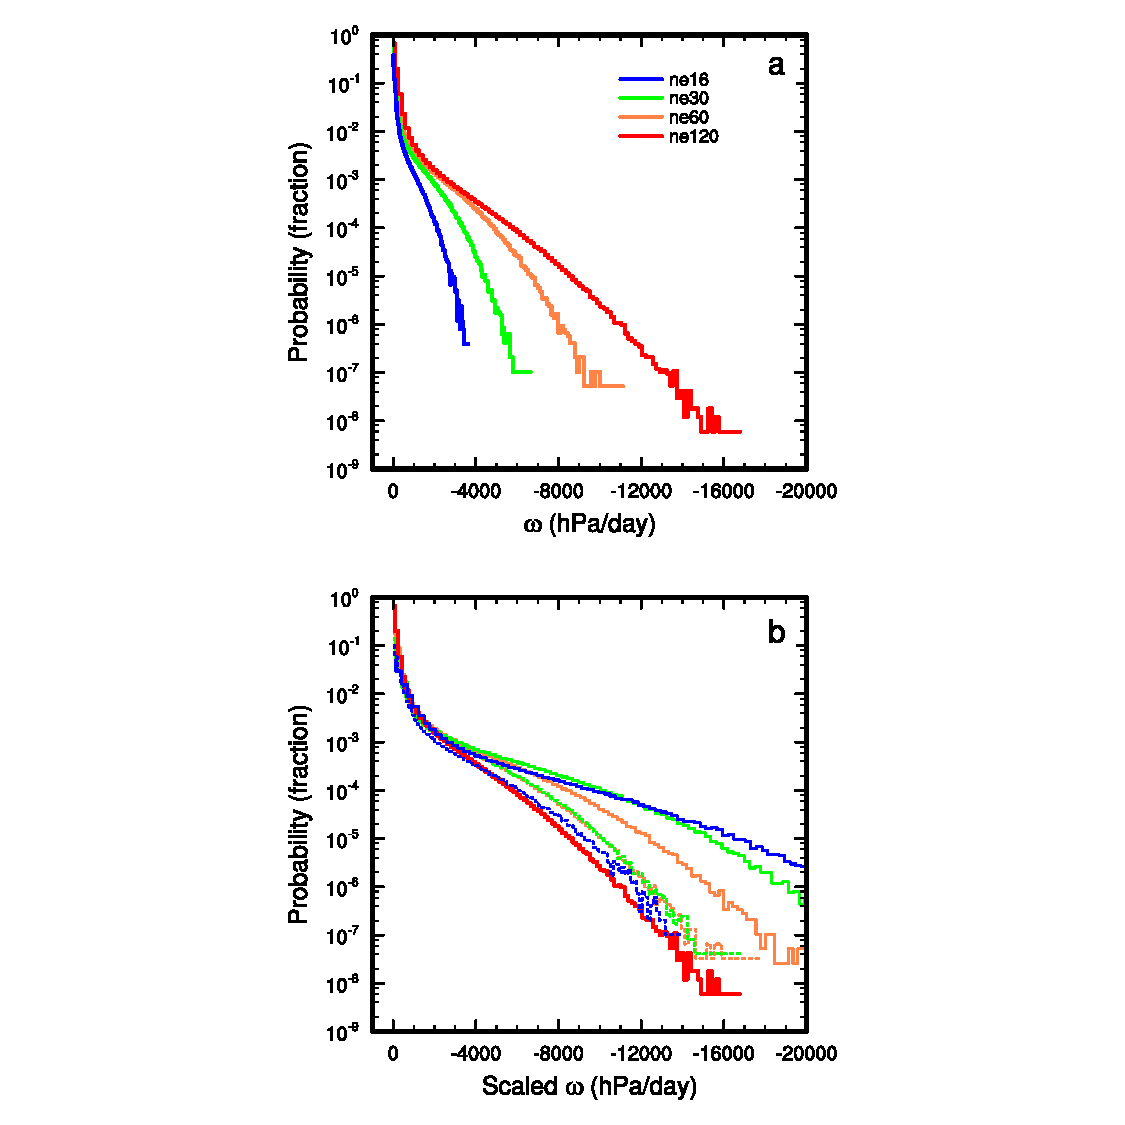
\includegraphics[width=20pc,angle=0]{chapter2/figure7.pdf}\\
\end{center}
\caption{(a) Probability density distributions of 600 hPa vertical pressure velocity conditionally sampled for upward motion in the region $10^{\circ}$ N to $10^{\circ}$ S. (b) Probability density distribution of vertical pressure velocities in (a) rescaled to the ne120 simulation using a $\Delta x^{-1}$ scaling (solid thin lines) and a $\Delta x^{-2/3}$ scaling (dotted thin lines). Values computed from 1460 instances of 6-hourly output randomly selected from the integration period.}
\label{fig:figure2-7}
\end{figure}

While we don’t expect the steady-state GCM solutions of vertical velocity to be linear in $k$, it is instructive to determine the degree to which the linear scaling reflects the full solution. To perform the scaling, we take the grid spacing, $\Delta x$, from the four simulations and scale the vertical velocities in the ne16, ne30 and ne60 simulations to the scale of the ne120 simulation using a $k \propto \Delta x^{-1}$ scaling. The probability density distribution of resolved upward motion in the deep tropics for all simulations are shown in Figure~\ref{fig:figure2-7}a, and the scaled distributions are provided in Figure~\ref{fig:figure2-7}b. The $\Delta x^{-1}$ relationship does a poor job of explaining the sensitivity of the resolved vertical motion to horizontal resolution, systematically over predicting the vertical velocities compared to the ne120 simulation.

The $\Delta x^{-1}$ scaling is an interpretation of the dispersion relation \citep{WK1982MWR}, but may also be derived from a scale analysis of the kinetic energy budget \citep{PG2006JAS} or the Poisson equation \citep{JR2016QJRMS}. Because of the the poor fit of the $\Delta x^{-1}$ scaling on the model solutions (Figure~\ref{fig:figure2-7}b), it might be tempting to abandon our explanation altogether. However, the physics of the $\Delta x^{-1}$ scaling has a strong theoretical foundation, and instead we reconcile our explanation with a modification. We argue that the linear Boussinesq scaling is reflective of what occurs in GCMs, but that additional processes, likely associated with parameterized moist processes and resulting feedbacks onto the general circulation, steer the solution away from a $\Delta x^{-1}$ scaling. 

\cite{RETAL2016CD} propose a shallower scaling exponent of $\Delta x^{-2/3}$. The  is the scaling that results from applying mass continuity to the $-5/3$  spectral slope of the horizontal winds typical of mesoscale circulations \citep{RETAL2016CD}. For comparison, the $\Delta x^{-2/3}$ scaling is overlain in Figure~\ref{fig:figure2-5}b. While the $\Delta x^{-2/3}$ scaling overestimates the vertical velocities compared to the ne120 simulation, the overestimate is much less than any single curve using the $\Delta x^{-1}$ scaling, and the scaled distributions all line up on top of one another. The \cite{RETAL2016CD} scaling is clearly a more accurate representation of the sensitivity of the fully coupled solution to horizontal resolution than that provided by linear Boussinesq theory.

\subsection{Conclusions}
We have studied the convergence of the mean state of the spectral element version of the Community Atmosphere Model (CAM) coupled to the version 4 physics package in an aqua-planet configuration. As the horizontal resolution is increased, the atmosphere progressively dries, cloud cover decreases and the large-scale precipitation rate increases at the expense of convective precipitation. Variations in the global atmospheric energy budget are primarily a reflection of these changes, resulting in a reduction in longwave cloud forcing and an increase in clear-sky transmissivity with resolution. The regional atmospheric energy budget indicates that large-scale precipitation increases are balanced by anomalous convergence of dry-static energy transport, due to increasing mean vertical velocities in the deep tropics. An analysis of the moisture budget reveals that the drying trend in the simulations is balanced by anomalous divergence of moisture fluxes associated with an intensification of the Hadley Cell and simultaneous changes to the extra-tropical circulation. The large reductions in cloud fraction with resolution are a result of a lower relative humidity field and reductions in activity of the convection scheme. 
 
A possible explanation for the resolution sensitivity of the mean state was formulated, inspired by the experiments of \cite{W1999T} and linear Boussinesq theory. We hypothesize that an increase in horizontal resolution leads to a reduction in horizontal scale of the diabatic forcing from the column physics, facilitating fine-scale flow and faster resolved convective updrafts within the dynamical core. Since buoyancy consumption is proportional to the magnitude of resolved upward motion, the dynamical core becomes more efficient at consuming buoyancy with resolution. As a result of the process ordering within CAM, and presumably other General Circulation Models \citep{B1991ECMWF}, the convection scheme may only remove buoyancy produced through large-scale precipitation after the dynamics have had an opportunity to consume of some of the buoyancy, which we speculate results in a reduction in activity of the convection scheme with resolution.

It is difficult to provide definitive proof of our explanation from an analysis of the aqua-planet experiments. We suggest that the reason for this difficulty is because the implied $\Delta x^{-1}$ dependence of the resolved vertical velocity elicits a non-linear response, pushing the full solution towards a new equilibrium that departs from $\Delta x^{-1}$ scaling. We have developed some simple deterministic dry experiments to test our hypothesis, using idealized diabatic forcing. Our results indicate that a $\Delta x^{-1}$ dependency is a robust feature of the spectral element dynamical core in CAM \citep{HR2018JAMES}. Future work will target how the inclusion of moist parameterizations effects the  scaling.

The strong coupling of the large-scale precipitation scheme with the dynamics at high horizontal resolution, but still within the hydrostatic regime, has been shown to be important for the simulation of Tropical Cyclones \citep{ZHL2012JAS} and precipitation extremes \citep{LETAL2011TELLUS,YETAL2014JCLIM,RETAL2016CD,OETAL2016JAMES}. Our explanation, if confirmed, implies that the interaction of the large-scale precipitation scheme with the dynamics is highly dependent on the horizontal resolution, and efforts to produce ‘scale-aware’ closures may need to focus on this interaction to preserve some of the benefits of high-resolution simulations.  \label{sec:chapter2}

\newpage
\begin{center}
\section{An idealized test of the response of the Community Atmosphere Model to near grid-scale forcing across hydrostatic resolutions}
%\chapter{\bf{\normalsize An idealized test of the response of the Community Atmosphere Model to near grid-scale forcing across hydrostatic resolutions}}
\end{center}
%\addcontentsline{toc}{section}{\protect\numberline{}An idealized test of the response of the Community Atmosphere Model to near grid-scale forcing across hydrostatic resolutions}
%\addcontentsline{toc}{chapter}{\protect\numberline{}An idealized test of the response of the Community Atmosphere Model to near grid-scale forcing across hydrostatic resolutions}
\subsection{Introduction}
The implementation of static or adaptive grid refinement in global atmospheric general circulation models (AGCMs) is a desirable, and increasingly common feature of next-generation atmospheric models. Regional grid refinement permits the explicit simulation of processes at the kilometric scale in a global model, providing a unification of global, regional and, in some cases, cloud-scale weather and climate simulations within a single AGCM framework \citep[e.g.,][]{LETAL2001MWR,WA2011MWR,RETAL2013JCLIM,Z2014QJRMS,ZetAl2014JCb,RHUZ2016,HETAL2016JCLIM}. This framework permits the interaction of the refined region with the globally resolved circulation, resulting in an autonomous representation of energy and enstrophy cascades \citep{C1971JAS,L1999JFM}, and global teleconnections \citep{WG1981MWR} that may affect the solution locally. 

The spectral element dynamical core option (CAM-SE) in the Community Atmosphere Model (CAM) has been designed to support variable resolution grids \citep{ZetAl2014JCb,GetAl2014GMD}. While CAM-SE is equipped with higher order numerics and local conservation properties to prevent degradation of the solution across highly distorted elements \citep{TF2010JCP,ZetAl2014JC,GetAl2014GMD}, the resolved vertical motion and precipitation rates exhibit an alarming sensitivity to grid-refinement \citep[e.g.,][]{RETAL2012ASL,YETAL2014JCLIM,ZetAl2014JCb,OETAL2016JAMES,HR2017JCLIM}. Although it is commonly accepted that the sensitivity of AGCM solutions to grid-refinement are related to the parameterization of moist physics, the exact mechanisms are not clearly identified. The difficulties of deciphering causes of diverging AGCM solutions under grid-refinement lie in the significant complexity of the models themselves. For example, it is quite common for an AGCM to have three distinctly separate schemes for predicting cloud amount \citep[e.g.,][]{PETAL2014JCLIM}. While there may be satisfactory reasons for this separation, and not withstanding recent advances in unified cloud schemes \citep{GETAL2002JAS,P2014JAS}, this complexity makes it difficult to unravel which component of which scheme, or interactions with other parts of the model, are contributing to the model’s behavior. 

An alternative explanation for the resolution sensitivity observed in AGCMs relates to the inherent scale dependencies of the underlying equations of motion \citep{F2007JAS,HR2017JCLIM}. These scale dependencies have been discussed before in the context of non-hydrostatic convection permitting simulations \citep{O1981JAS,WETAL1997MWR,PG2006JAS,JR2016QJRMS}, but its relevance to hydrostatic convection in AGCMs is rarely discussed \citep{F2007JAS,J2017JAMES}. This is hardly surprising since convection schemes are implemented in AGCMs to reduce the occurrence of resolved convection, and may lead many to question whether resolved convection occurs in AGCMs at all. However, evidence showing the importance of resolved updrafts and downdrafts on simulated tropical convective systems in AGCMs can be found as far back as \cite{MK1997QJRMS}, and more recently by \cite{OETAL2016JAMES}.

\begin{figure}[t]
\begin{center}
\noindent\includegraphics[width=25pc,angle=0]{chapter3/Figure1.eps}\\
\end{center}
\caption{Instantaneous snapshot of the vertical pressure velocity (colors) and the diabatic forcing from the column physics (black contours) for a longitude-height transect at the equator from a series of aqua-planet simulations at four different horizontal resolutions. Contour interval is $+10$ K day$^{-1}$ (solid) and $-10$ K day$^{-1}$ (dashed).}
\label{fig:figure3-1}
\end{figure}

Figure~\ref{fig:figure3-1} illustrates the prevalence of resolved updrafts in an AGCM. The simulations are from a series of CAM-SE aqua-planet simulations \citep[following][]{NH2000ASL} at four different horizontal resolutions typical of present day AGCMs. The only parameters varied in the simulations are the dynamics time-step and hyper-viscosity coefficients, and the physics time-step is set to 1800 s for all resolutions (Table~\ref{tbl:table3-1}). All other aspects of the simulations are identical to the aqua-planet reference simulation described in \cite{MWO2016JAMES}. Instantaneous snapshots of the vertical pressure velocity in the longitude-pressure plane at the equator for four different quasi-uniform horizontal resolutions are overlain by contours of large-magnitude, instantaneous diabatic forcing from the column physics. Resolved updrafts and downdrafts, primarily a response to grid-scale ``thermals" and re-evaporation of falling condensate by the large-scale condensation scheme, populate the deep tropics and are a crucial component of the tropical circulation \citep{HR2017JCLIM}. 

What is also clear from Figure~\ref{fig:figure3-1} is that the magnitude of the vertical motion, as well as the horizontal scale of the diabatic forcing and resolved convective elements as a whole, has some proportional relation to the grid spacing. The global power spectrum of the diabatic forcing arising from the column physics in the simulations (Supplementary Figure~\ref{fig:sfigure3-1}) provides conclusive evidence for a reduction in diabatic forcing scale with resolution. As discussed in \cite{HR2017JCLIM}, the relationship between the horizontal scale of the buoyancy forcing, and the magnitude of the vertical velocity is consistent with the equations of motion. To illustrate this point, we proceed with a scale analysis of the non-rotating, dry equations of motion in the anelastic framework described in \cite{JR2016QJRMS}.

\cite{JR2016QJRMS} augment the conventional anelastic approximation with a few important modifications. The first modification is that the full pressure is split between a locally balanced hydrostatic pressure, $p_{HYD}$, and a non-hydrostatic residual \citep{D1979JAS}. The second modification is the introduction of the effective buoyancy, $\beta$. The effective buoyancy is the vertical acceleration that would result from zeroing out the wind field, which is useful for isolating the component of vertical acceleration due to the Archimedean buoyancy. \cite{JR2016QJRMS} then introduce the buoyancy pressure, $p_{\beta}$, which is the residual non-hydrostatic pressure associated with zeroing out the wind field, the vertical gradient of which is the effective buoyancy. These modifications lead to the Poisson equation \citep[equation 8 in][]{JR2016QJRMS}:
\begin{equation}
-\nabla (p_{\beta}) = \nabla^{2}_{h} (p_{HYD}),\label{eq:eq3-1}
\end{equation} 
where $\nabla^2$ is the Laplacian operator ($\nabla^{2}_{h} + \frac{d^2}{dz^2}$) and $\nabla^{2}_{h}$ is ($\frac{d^2}{dx^2} + \frac{d^2}{dy^2}$). Consider a vertical column of air of diameter $D$ and height $H$, and constant Archimedean buoyancy $B_0$ throughout, then after taking the vertical derivative of equation~\ref{eq:eq3-1}, the scale analysis for $\beta$ is: 
\begin{equation}
\beta = B_0 \left[ D^2 \left( \frac{1}{D^2} + \frac{1}{H^2} \right) \right]^{-1},\label{eq:eq3-2}
\end{equation}
\citep[compare to equation 10 in][]{JR2016QJRMS}. Setting the scale of $\beta$ to $W/T$, where $W$ is a vertical velocity scale and $T=H/W$, and noting that at hydrostatic scales $\frac{1}{D^2}  \ll \frac{1}{H^2}$, solving for $W$:
\begin{equation}
W = \sqrt{B_0 H} \frac{H}{D}. \label{eq:eq3-3}
\end{equation}
The vertical velocity scale due to the Archimedean buoyancy is inversely proportional to the horizontal scale of the Archimedean buoyancy, at hydrostatic scales. Inspection of the Poisson equation (equation~\ref{eq:eq3-1}) indicates that the $1/D$ scaling is a result of the horizontal scale of the hydrostatic pressure perturbation, which drives convergence into the air column and vertical motion. The horizontal scale of the hydrostatic pressure perturbation is set by the horizontal scale of the Archimedean buoyancy \citep{JR2016QJRMS}, and determined by the horizontal scale of the diabatic forcing.

Through assuming a linear relationship between grid spacing ($\Delta x$) and diabatic forcing scale, which remains untested, but which \cite{J2017JAMES} has shown evidence for at cloud-permitting resolutions, one may expect the variations in vertical velocity to go like $\Delta x^{-1}$. However, a $\Delta x^{-1}$ relationship, while consistent with the general trend of greater vertical motion at higher resolution (e.g. Figure~\ref{fig:figure3-1}), overestimates the resolution sensitivity observed in a series of CAM-SE aqua-planet simulations analyzed in \cite{HR2017JCLIM}. The simulations depicted in Figure~\ref{fig:figure3-1} are similar – the  $\Delta x^{-1}$ scaling overestimates the sensitivity to horizontal resolution (Figure~\ref{fig:figure3-10}, dashed lines). The $\Delta x^{-1}$ scaling may be incorrect simply because the relationship between diabatic forcing scale and $\Delta$ is non-linear. Alternatively, through maintaining the linear relationship between forcing scale and $\Delta x$, \cite{HR2017JCLIM} propose that feedbacks within other components of the AGCM steer the solution towards a weaker resolution sensitivity.
 
The goal of this paper is to test the robustness of the scaling (equation~\ref{eq:eq3-3}) in a simplified, non-rotating AGCM framework. We begin with an idealized set of rising thermal bubbles using CAM-SE without moist processes, and incrementally introduce some moist parameterizations to determine how their inclusion may affect the scaling of equation~\ref{eq:eq3-3}. We do not consider the influence of convection schemes – CAM convection schemes are incompatible with our experimental design. While this limits our ability to extend our results to the behavior of a complete AGCM, we argue that our simplified moist framework is still relevant to the behavior of a complete AGCM, and as such, will shed light on whether the moist physics or the scale dependencies of the dry equations of motion are the driving force behind the resolution sensitivity in CAM. 

\begin{table}
\begin{center}
\noindent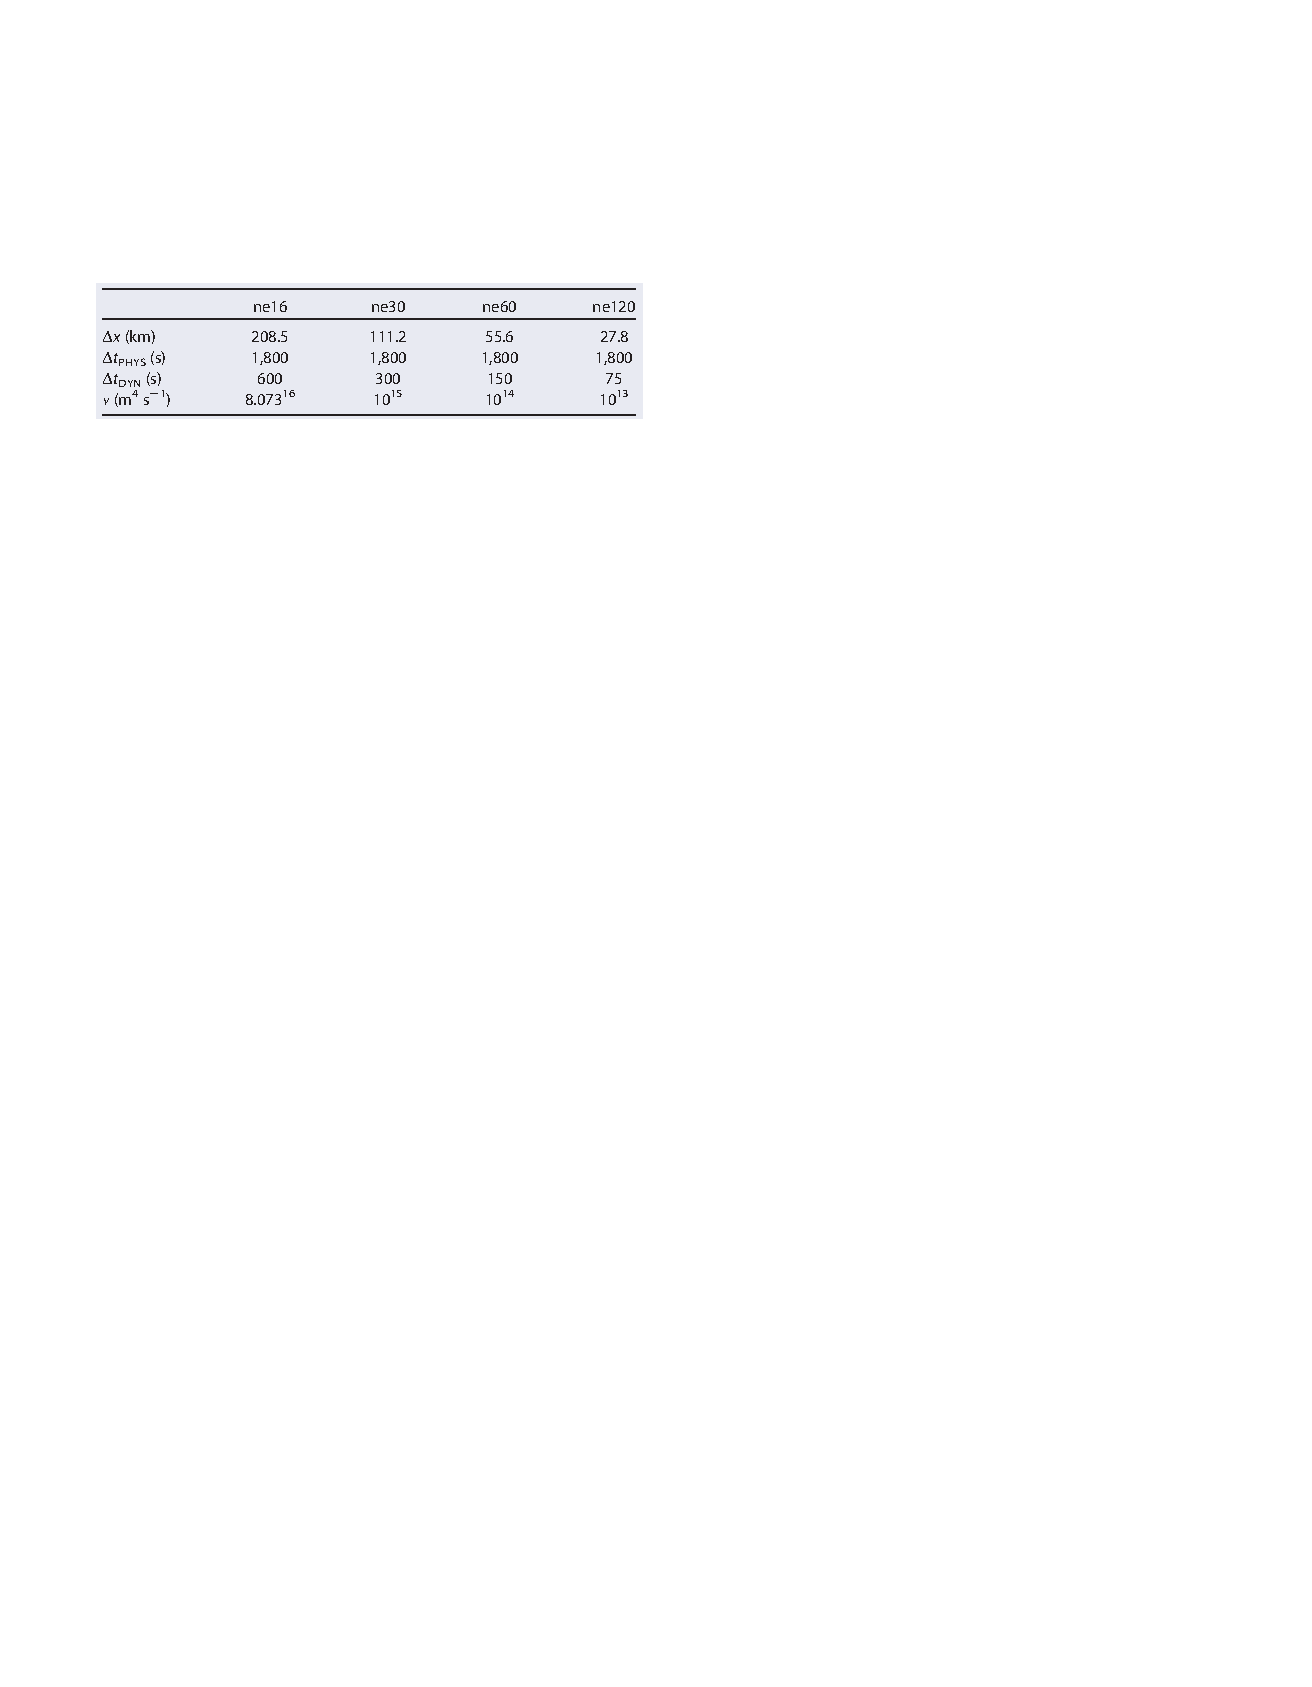
\includegraphics[width=25pc,angle=0]{chapter3/table1.pdf}\\
\end{center}
\caption{Quasi-uniform horizontal grid spacing ($\Delta x$), time-stepping ($\Delta t$) and hyper-viscosity coefficients ($\nu$) used in the aqua-planet simulations. Hyper-viscosity coefficients are after \cite{ZetAl2014JC} and are identical for the treatment of momentum, temperature and specific humidity.}
\label{tbl:table3-1}
\end{table}

Rising bubble experiments are commonly used to test atmospheric models, although they are disproportionately used in non-hydrostatic models, often resembling an idealized thermal with horizontal scales on the order of a kilometer or less \citep{KW_1978JAS,GETAL1991JAS,BETAL2002MWR,JR2016QJRMS}. The focus of this study is on bubbles of hydrostatic scale, and are intended as a surrogate grid-scale thermal occurring in more complex AGCM configurations (e.g., Figure~\ref{fig:figure3-1}). Section 3.2 provides an overview of the dynamical cores and moist physical parameterizations used throughout the paper, and a description of the analytical initial conditions. Section 3.3 presents the results of the experiments, Section 3.4 contains a discussion of the results and section 3.5 provides some concluding thoughts.

\subsection{Materials and Methods}
\subsubsection{Dynamical Cores}
For most of our experiments, we choose to work with the spectral element dynamical core option of the Community Atmosphere Model \citep[CAM-SE;][]{DetAl2012IJHPCA}, the atmospheric component of the Community Earth System Model, version 1.2. CAM-SE solve the vector-invariant hydrostatic primitive equations using a fourth-order accurate, continuous Galerkin method on the sphere. A brief overview of the CAM-SE dynamical core is provided in \cite{HR2017JCLIM}, and further details are available in the model documentation \citep{CAM5}. The version of CAM-SE used in this study is more recent than for the simulations analyzed in \cite{HR2017JCLIM}, with the main distinction being the change to a third-order accurate, five-stage Runge Kutta time-stepping scheme \citep{DetAl2012IJHPCA,GU2016GMD}.

CAM-SE uses an unstructured, cubed-sphere grid. For the quasi-uniform grid used in this study, the notation for the cubed-sphere grid is abbreviated by the number of elements along the edge of one of the six cubed-sphere panels. The grid used in this work contains 30 elements along the edge of a cubed-sphere face (abbreviated as ‘ne30’). Since each element contains 4 interior Gauss-Lobatto-Legendre (GLL) quadrature nodes, and 12 GLL nodes along the (shared) element boundary, the ne30 simulations correspond to an average horizontal grid-spacing of 111.2 km. The CAM-SE dynamical core contains no implicit dissipation in the horizontal, and so fourth-order hyper-viscosity operators are applied to state variables to suppress numerical artifacts \citep{DetAl2012IJHPCA}. The resolution dependent hyper-viscosity coefficients used throughout this study are the same as those used for the aqua-planet experiments provided in Table~\ref{tbl:table3-1}, and are from \cite{ZetAl2014JC}.

Experiments are also performed using the finite-volume dynamical core in CAM \citep[CAM-FV;][]{L2004MWR,CAM5}. CAM-FV solves for the horizontal dynamics using a finite-volume formulation of the vector invariant primitive equations \citep{LR1997QJR}. Like CAM-SE, CAM-FV utilizes the “Vertically Lagrangian” method \citep{L2004MWR}, solving the horizontal dynamics within floating hybrid sigma-pressure surfaces, and periodically remapping the state back to a Eulerian, vertical reference coordinate \citep{CAM5}. CAM-FV contains implicit dissipation of scalars quantities, which includes vorticity, and explicit divergence damping is applied to the divergent winds. Both CAM-SE \citep{DetAl2012IJHPCA}, and CAM-FV \citep{L2011IJHPC,WJRL2010MWR} contain default fourth-order divergence damping, but to promote a larger diversity in design choices between the two dynamical cores, the second-order divergence damping option is used in CAM-FV \citep{CAM3}. However, sensitivity experiments will be discussed that quantify the effect of the order of the divergence damping operator in CAM-FV. The dynamics are solved on a latitude-longitude grid, and necessitates a polar filter to stabilize solutions in polar regions \citep{CAM5}. A standard grid with a horizontal resolution of $0.9^{\circ}$ latitude by $1.25^{\circ}$ longitude (nominally $1^{\circ}$), equivalent to an average equatorial grid spacing of 139 km, is used in all CAM-FV experiments.

The vertical resolution is the same for all grids in this study (regardless of dynamical core), consisting of 30 unequally spaced, hybrid sigma-pressure levels \citep{CAM5}. Higher horizontal resolution grids are obtained by reducing the Earth-like planetary radius to match the resolution of other grid configurations, as in \cite{RM2016GRL}. Modifications to the Coriolis parameter are not required - only non-rotating planets are considered in this study. For all experiments described in this paper, a dynamics time-step of 75 seconds and 56.26 seconds are used in CAM-SE and CAM-FV, respectively, which satisfy the stability constraints of the highest resolution grids used throughout the study. The motivation for fixing the dynamics time-step, regardless of horizontal resolution, is in part for simplicity, but also to generalize our results to the behavior of the variable resolution version of CAM-SE. The variable resolution version of CAM-SE requires the time-step to be equal everywhere on the grid, and must be chosen to satisfy the Courant number in the refined region \citep{ZetAl2014JC}.

\subsubsection{Moist Physics}
The moist experiments contain water species and parameterizations of moist processes. Water species are transported by the dynamical core, and the parameterizations are computed at the end of every third dynamics time-step in CAM-SE, and every fourth dynamics time-step in CAM-FV, equivalent to a physics time-step of 225 s. Further details on the coupling of the dynamical cores to the physical parameterizations is described in \cite{HR2017JCLIM} and \cite{CAM5}. We experiment with parameterizations that are intended to span the spectrum of complexity. In the least complex case, the dynamical cores are coupled to the large-scale condensation scheme of the ‘simple physics’ package of \cite{RJ2012JAMES}, which we refer to as ‘simple condensation’ throughout the manuscript. This warm-rain scheme assumes all condensates are immediately removed from the column with no cloud phase.

Towards the other end of the spectrum, the Community Atmosphere Model, version 5 physics package \citep[CAM5;][]{CAM5} contains a stratiform cloud scheme, with separate macrophysical \citep{PETAL2014JCLIM} and microphysical \citep{MG2008JC} routines that together, constitute a more complex large-scale condensation scheme. The stratiform scheme computes ice and liquid cloud phases through prognostic equations for cloud droplet number and concentration, and contains an explicit representation of falling hydrometeors \citep{MG2008JC}. As in the aqua-planet reference simulations presented in \cite{MWO2016JAMES}, the cloud liquid and cloud ice concentrations are held to constant values ($100 \times 10^6$ m$^{-3}$ and $0.1 \times 10^6$ m$^{-3}$, respectively) to suppress dependencies on aerosol species, which are not present in our simulations. As a final level of complexity, we couple the stratiform scheme with the downgradient vertical dissipation routine used in CAM5 for the free troposphere, which diffuses momentum, temperature and specific humidity using standard mixing length and Richardson number dependent formulations \citep{CAM4}.

\begin{figure}
\begin{center}
\noindent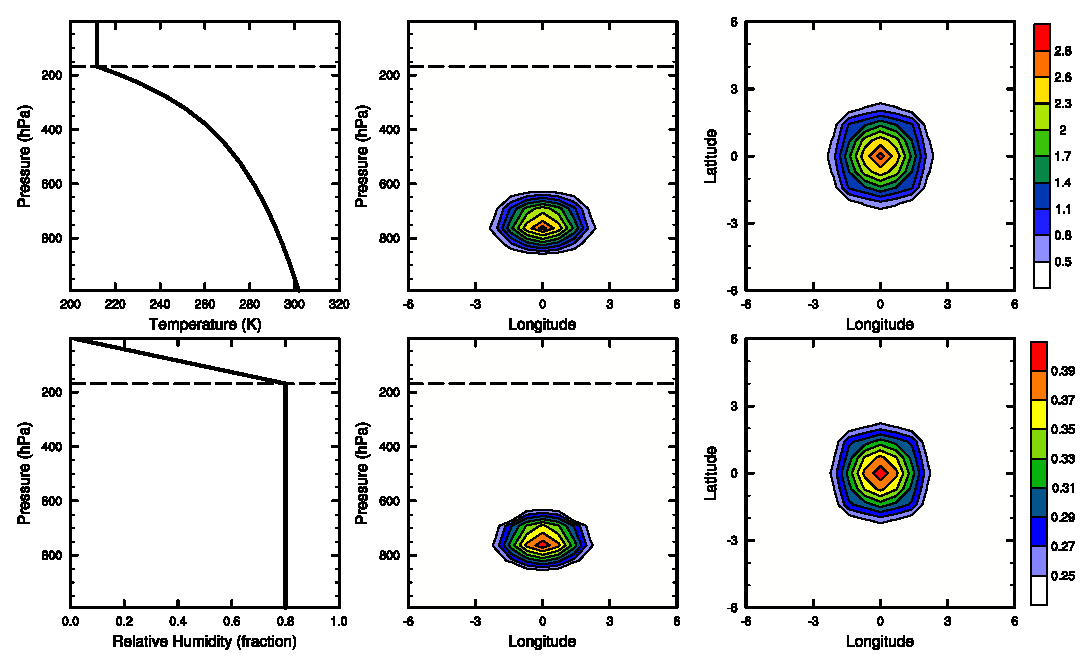
\includegraphics[width=25pc,angle=0]{chapter3/Figure2.eps}\\
\end{center}
\caption{Initial conditions used in the moist experiments. Background temperature (top, left) and background relative humidity (bottom, left) reference profiles.  A moist bubble with $r_h = X \times 350$ km, where $X$ is the scale factor from Table~\ref{tbl:table3-2}, is depicted in the middle and right plots: potential temperature perturbation in the longitude-pressure plane (top, middle) and the latitude-longitude plane (top, right) and the relative humidity perturbation in the longitude-pressure plane (bottom, middle) and the latitude-longitude plane (bottom, right). The horizontal dashed lines denotes the location of the tropopause.}
\label{fig:figure3-2}
\end{figure}

\subsubsection*{Initial Conditions}
The experiments are designed to isolate the scale sensitivity expressed in complex, moist AGCM resolution experiments, such as in Figure~\ref{fig:figure3-1}. The general procedure is to produce a set of approximately one-day long simulations of a rising thermal bubble in an idealized tropical environment, each bubble having its horizontal radius, $r_h$, and model horizontal grid-spacing, $\Delta x$, simultaneously reduced by a proportionality factor, $X$, to be defined later. An implicit assumption of this experimental design is that the forcing scale, $2 r_h$, is linear in $\Delta x$. 

The background temperature and moisture profiles are inspired by the thermodynamic structure of strongly convecting regions in the deep tropics of the aqua-planet simulations, and are similar to the neutrally stable conditions proposed by \cite{BETAL2002MWR}. The background temperature profile is a horizontally uniform, reversible moist adiabat pertaining to a surface temperature, $T_0$, and constant relative humidity with height, $h_0$. The tropopause pressure is the hydrostatically balanced pressure corresponding to a fixed height of 15 km, above which the temperature and specific humidity are set to the tropopause values (Figure~\ref{fig:figure3-2}).

A temperature perturbation is introduced following \cite{KETAL2015JAMES}:
\begin{equation}
T^{\prime} (R) = \begin{cases} \Delta \theta * \Pi * \cos^2 (R \frac{\pi}{2}) \: for \: R \leq 1 \\
						0 \; \; \; \; \; \; \; \; \; \; \; \; \; \; \; \; \; \; \; \; \; \; \; \; \; \; \; for \:R > 1 \end{cases}, \label{eq:eq3-4}
\end{equation}
with magnitude $\Delta \theta$. $\theta$ is the potential temperature, $\Pi = (p/p_0)^{\kappa}$ is the exner function and $\kappa = R_d/c_{pd}$, where $g$ is the gravitational acceleration, $R_d$ is the gas constant for dry air, $c_{pd}$ is the specific heat capacity of dry air at constant pressure and $p$ is the pressure. 
\begin{equation}
R(r,z) = \left[ \left( \frac{r}{r_h} \right)^2 + \left( \frac{z-z_c}{r_z} \right)^2 \right]^{\frac{1}{2}}, \label{eq:eq3-5}
\end{equation}
where $r_h$ is again the horizontal bubble radius, $r_z$ the vertical radius. The great circle distance, $r$ , from central latitude $\phi_c$ and central longitude  $\lambda_c$ is
\begin{equation}
r(\phi_c, \lambda_c) = a * \cos^{-1} \left( \sin(\phi_c) \sin(\phi) + \cos(\phi_c) \cos(\phi) * \cos(\lambda - \lambda_c) \right), \label{eq:eq3-6}
\end{equation}
where $a$ is the planetary radius. The hydrostatically balanced reference height, $z$, is found through vertical integration of the hydrostatic relation, and $z_c$ is the location of the bubble center in the vertical. A relative humidity perturbation is collocated with the temperature perturbation, and is of the form:
\begin{equation}
RH^{\prime} (R) = \begin{cases} \left( 1 - h_0 \right) + \Delta h * \Pi * \cos^2 (R \frac{\pi}{2}) \: for \: R \leq 1 \\
						0 \; \; \; \; \; \; \; \; \; \; \; \; \; \; \; \; \; \; \; \; \; \; \; \; \; \; \; \; \; \; \; \; \; \; \; \; \; \; \; \; \; \; \; \; for \:R > 1 \end{cases}, \label{eq:eq3-7}
\end{equation}
where $\Delta h$ is the magnitude of the relative humidity perturbation above saturation. The relative humidity parameters are set to $h_0 = 0.80$ and $\Delta h  = 0.20$ (relative humidity is defined as a fraction as opposed to a percent, throughout this work) modeled after the aqua-planets. The definition of relative humidity in the initial conditions needs to be made consistent with the parameterization one is using. The simple condensation scheme and the CAM5 physics package use different definitions for saturation vapor pressure, and their initial conditions were made consistent with these definitions.

\begin{table}
\begin{center}
\noindent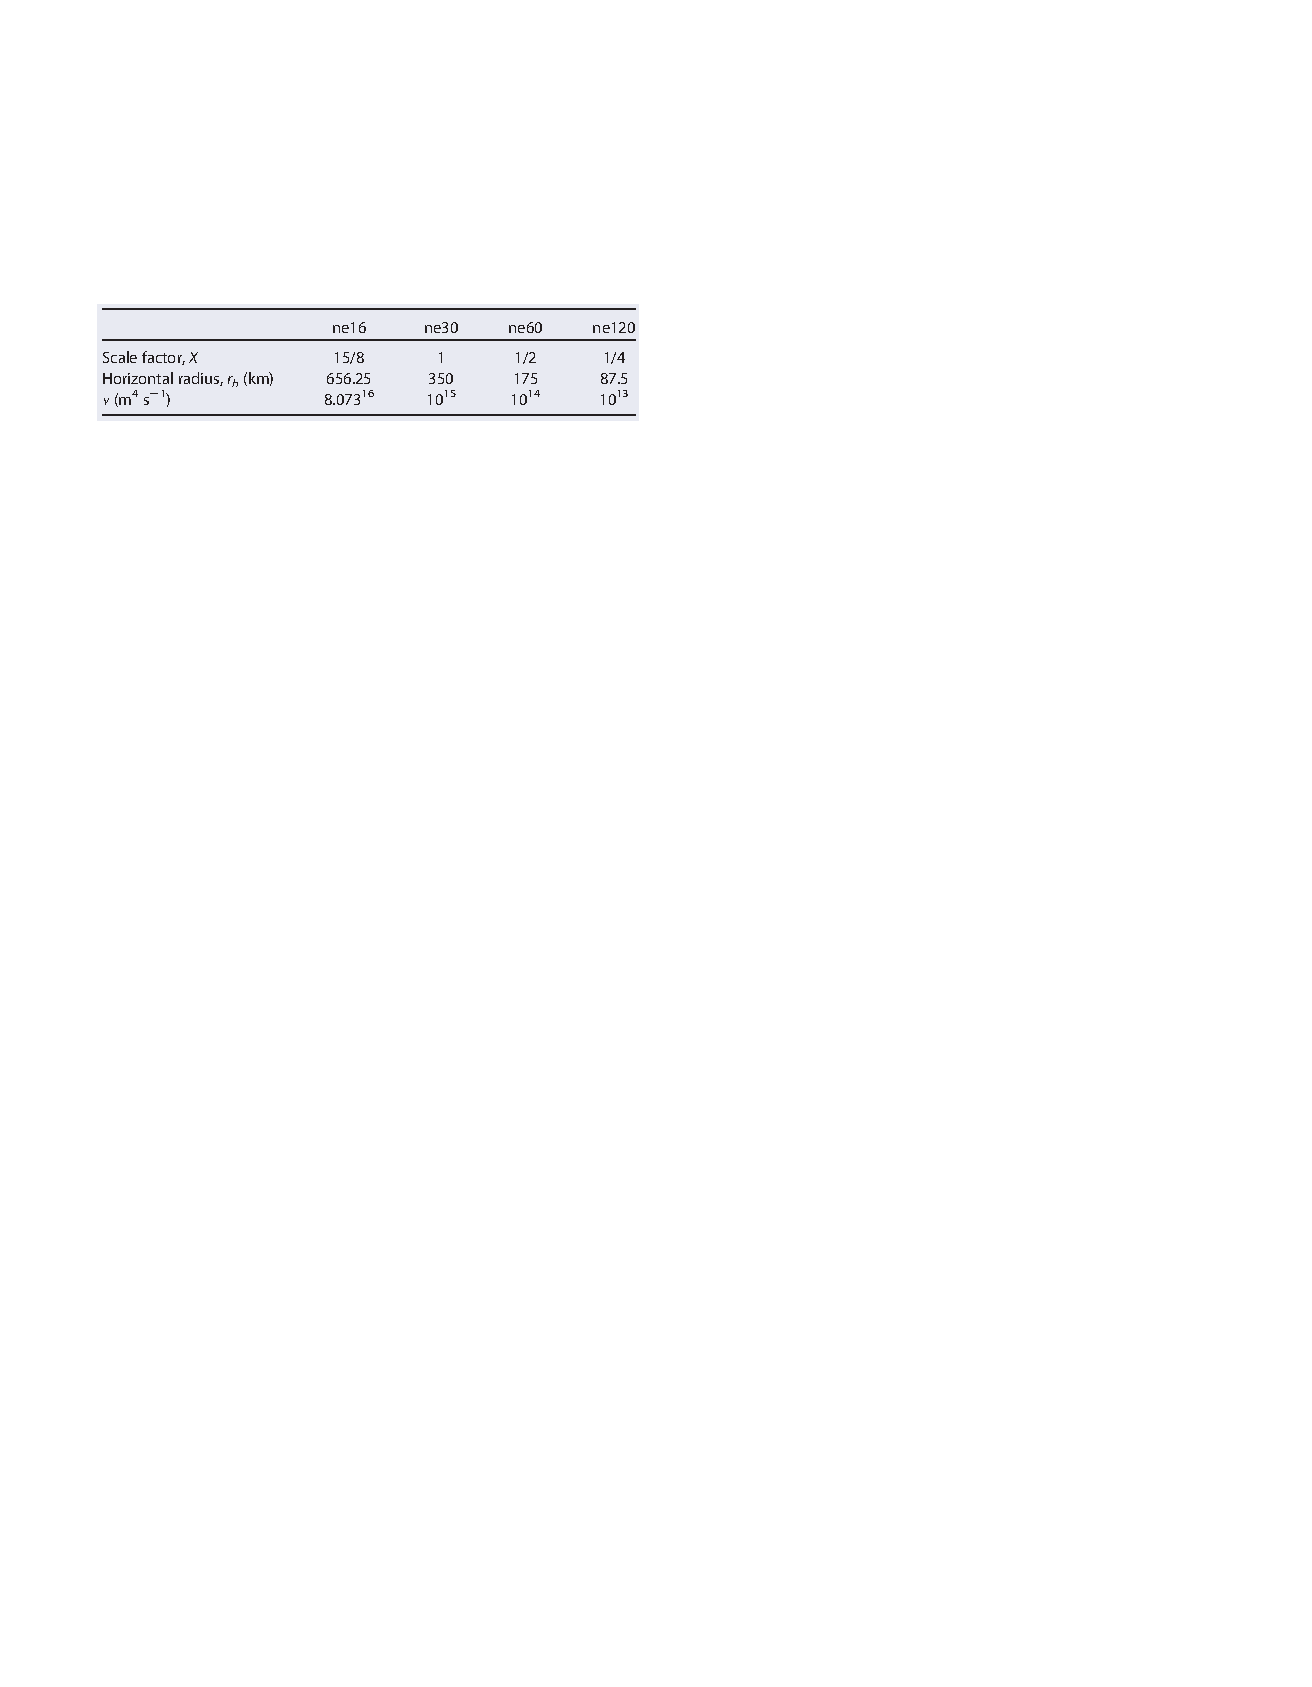
\includegraphics[width=25pc,angle=0]{chapter3/table2.pdf}\\
\end{center}
\caption{Scale factors ($X$) used to scale Earth’s planetary radius to match the horizontal resolution of other grids (header), as well as the horizontal bubble radius ($r_h$) and hyper-viscosity coefficients ($\nu$), for each equivalent resolution.}
\label{tbl:table3-2}
\end{table}

Through fixing the initial conditions, and multiplying the planetary radius, $a$, by the scale factor $X$, $r_h$ is varied by the same factor as $\Delta x$. In the style of \cite{RM2016GRL}, the scale factors are defined as the coefficients required to scale the Earth’s planetary radius to match the horizontal resolutions used in the aqua-planet simulations (Table~\ref{tbl:table3-2}). We set the horizontal diameter of the moist bubbles to about seven times the grid spacing (specifically, we set $r_h = 350$ km at Earth’s planetary radius) and a vertical diameter of 4 km ($r_z = 2$ km), which is comparable to the horizontal and vertical scales of diabatic forcing in the aqua-planet simulations (Figure~\ref{fig:figure3-1}). 

Two additional important parameters are the vertical location of the bubble ($z_c$) and the magnitude ($\Delta \theta$). A smaller $z_c$ or larger $\Delta \theta$ both lead to increased available potential energy, and potentially greater vertical motion. Figure~\ref{fig:figure3-1} indicates that large-magnitude stratiform tendencies are common in the Tropical upper-troposphere at all resolutions. The diabatic forcing depicted in Figure~\ref{fig:figure3-1} correspond to potential temperature perturbations on the order of 1 K. Despite the prevalence of the upper-troposphere structures, we opt for a more extreme initial condition, one that is less common in the simulations, to encourage non-linearity that could potentially break the scaling of equation~\ref{eq:eq3-3}. Plots of the initial conditions for the moist experiments are provided in Figure~\ref{fig:figure3-2}, depicting a bubble with a magnitude of 3K, a vertical extent much less than the depth of the troposphere, and located just above the nominal boundary layer. Table~\ref{tbl:table3-3} provides a list of all parameters used to generate the initial conditions for the experiments.

\begin{table}
\begin{center}
\noindent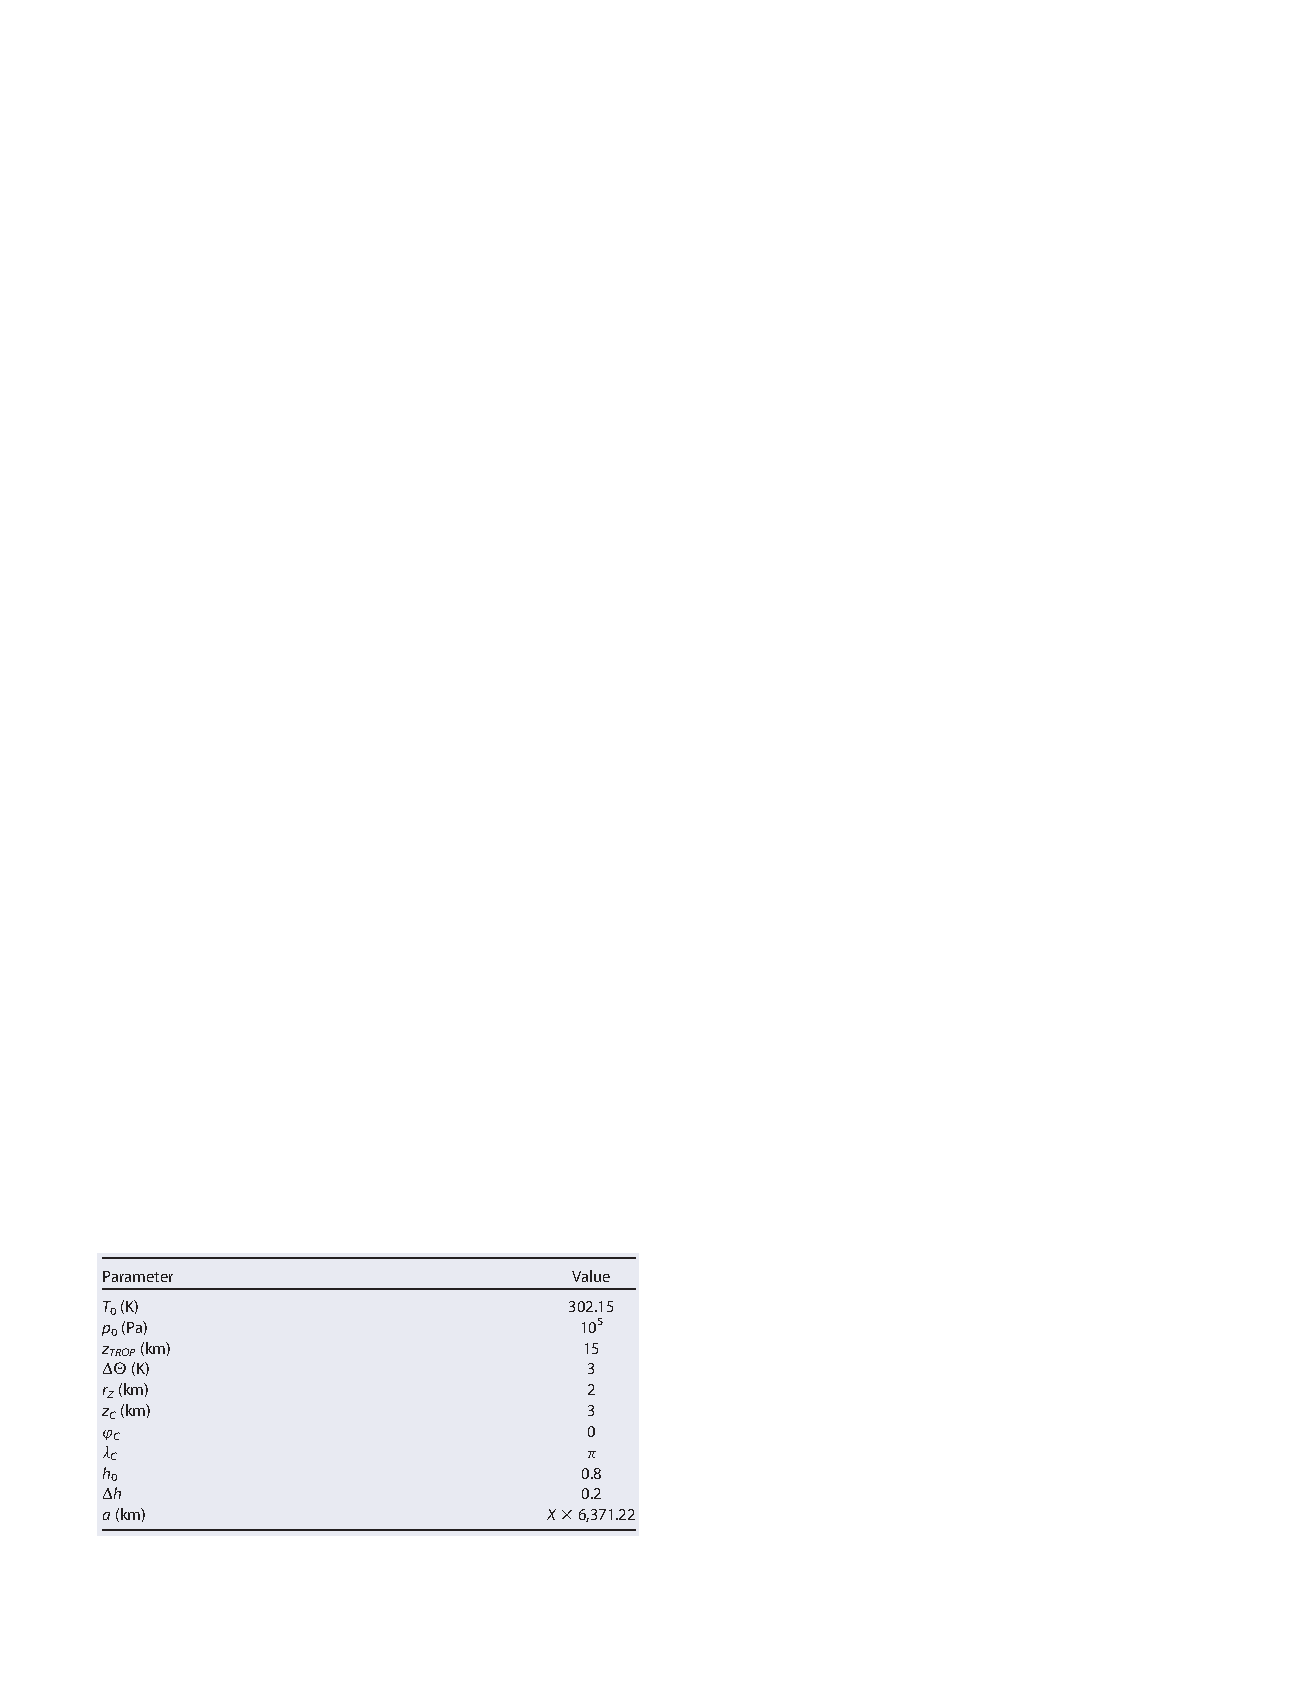
\includegraphics[width=20pc,angle=0]{chapter3/table3.pdf}\\
\end{center}
\caption{Parameters used in generating the initial conditions for the dry and moist experiments. $X$ is the scale factor, provided in Table~\ref{tbl:table3-2}.}
\label{tbl:table3-3}
\end{table}

\begin{figure}
\begin{center}
\noindent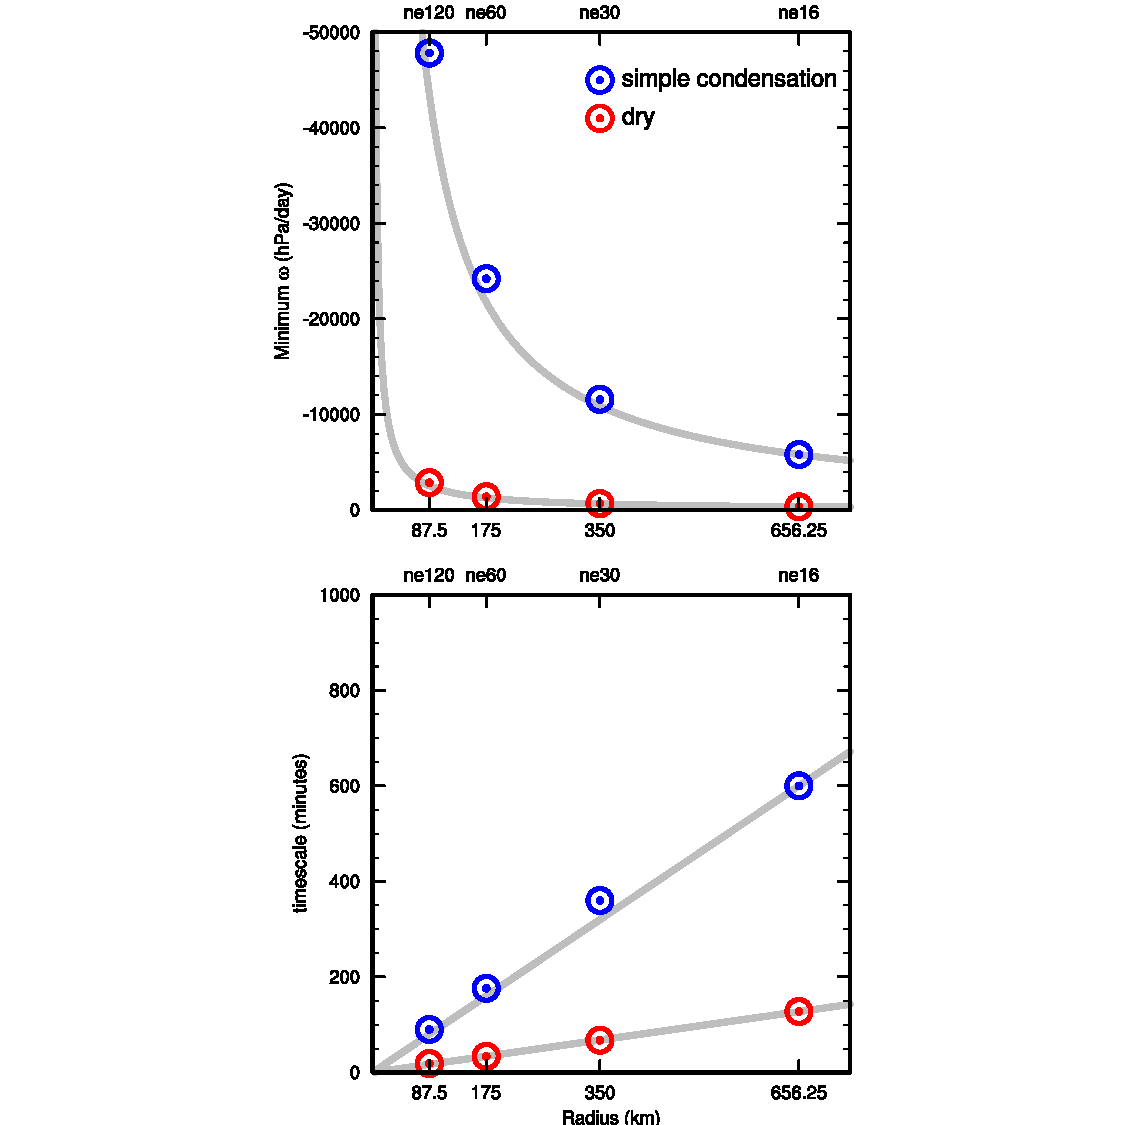
\includegraphics[width=20pc,angle=0]{chapter3/Figure3_crop.pdf}\\
\end{center}
\caption{Results of the experiments using the simple condensation scheme and an equivalent configuration without moisture (`dry’). (Top) minimum vertical pressure velocity, $\omega$, over the duration of each experiment as a function of bubble radius (Bottom) the model time associated with the minimum in $\omega$ as a function of bubble radius. The top axis indicates the equivalent horizontal resolution of the grid used to simulate a particular bubble radius. Grey lines represent the scaling of equation~\ref{eq:eq3-3}, scaled by the lowest resolution (ne16) solution.}
\label{fig:figure3-3}
\end{figure}

\subsection{Results}
\subsubsection{CAM-SE without moisture}
Before embarking on an analysis of the moist experiments, we first consider the behavior of an experiment which contains no moist processes. The red markers in Figure~\ref{fig:figure3-3} are the results of a dry experiment, i.e. the initial conditions are those of Figure~\ref{fig:figure3-2}, but with no specific humidity. The blue markers are the results from a moist experiment, and are discussed in the next section. Results are displayed as the minimum vertical pressure velocity, $\omega$, over the duration of each experiment as a function of $r_h$. The $1/r_h$scaling implied by equation~\ref{eq:eq3-3} is overlain as a grey line, scaled by the lowest resolution simulation. The analytical scaling and the model experiments agree to a remarkable extent, indicating that the model dynamics are adequately described by the simple scale analysis of equation~\ref{eq:eq3-3} for the case of a dry, rising bubble.

\begin{figure}
\begin{center}
\noindent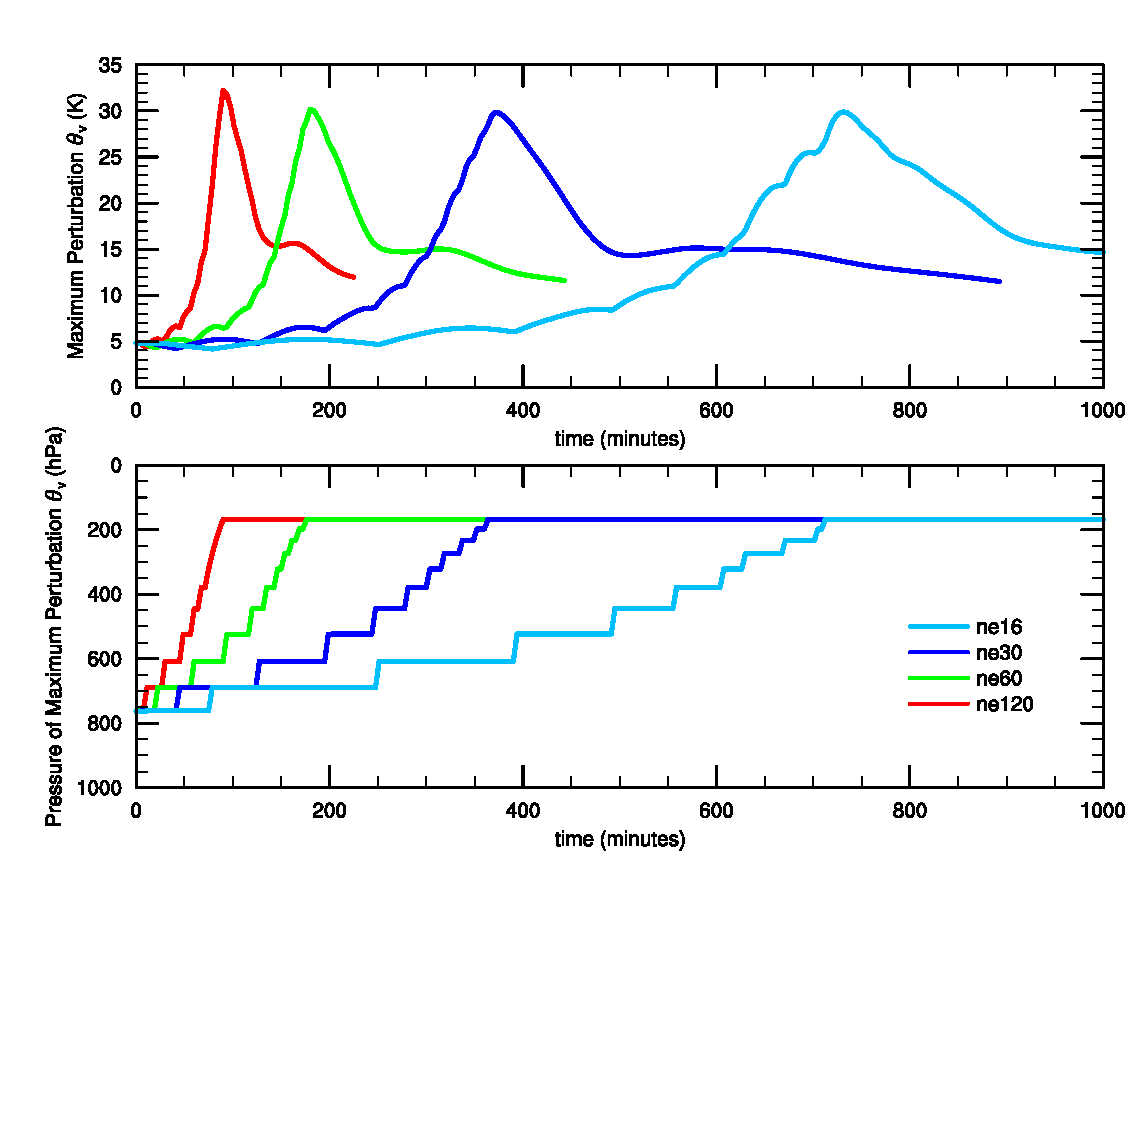
\includegraphics[width=25pc,angle=0]{chapter3/Figure4_crop.pdf}\\
\end{center}
\caption{Time series of the maximum perturbation $\theta_v$ (top) and the pressure associated with this maximum (bottom) in the moist experiment using the simple condensation scheme.}
\label{fig:figure3-4}
\end{figure}

\subsubsection{CAM-SE coupled to the Simple Condensation Scheme}
Figure~\ref{fig:figure3-3} also shows the results of the moist experiment with CAM-SE coupled to the simple condensation scheme. The simple moist experiments obey the linear scaling of equation~\ref{eq:eq3-3}, despite the inclusion of moist processes. This is not a trivial result since the analytical scaling (equation~\ref{eq:eq3-3}) was derived without any treatment of moist processes. Moisture does however amplify the vertical motion by about an order of magnitude compared to the dry case, with $\omega$ approaching $-50 \times 10^3$ hPa day$^{-1}$, or about 20 m s$^{-1}$. Whereas the dry bubbles are unable to reach the tropopause, the moist bubbles maintain their structures all the way to the tropopause, owing to a much larger reservoir of available potential energy.
 
The minimum vertical pressure velocities in the moist tests are attained once the moist bubble reaches the tropopause. This can be determined by comparing the timescales in Figure~\ref{fig:figure3-3} to the time evolution of the bubble pressure (Figure~\ref{fig:figure3-4}). Figure~\ref{fig:figure3-4} also shows that the minimum in $\omega$ are associated with a maximum virtual potential temperature ($\theta_v$) perturbation, defined as the difference in $\theta_v$ from the initial reference state. The maximum $\theta_v$ perturbation is approximately invariant to bubble radius, indicating the difference in $\omega$ across resolutions are almost entirely a result of the $1/r_h$ scaling, as opposed to a change in available potential energy ($\sqrt{B_0 H}$ in equation~\ref{eq:eq3-3}). The scaling fits the moist experiments well since the horizontal scale of the moist bubbles do not change significantly as they ascend to their level of neutral buoyancy (i.e., the tropopause).

\begin{figure}
\begin{center}
\noindent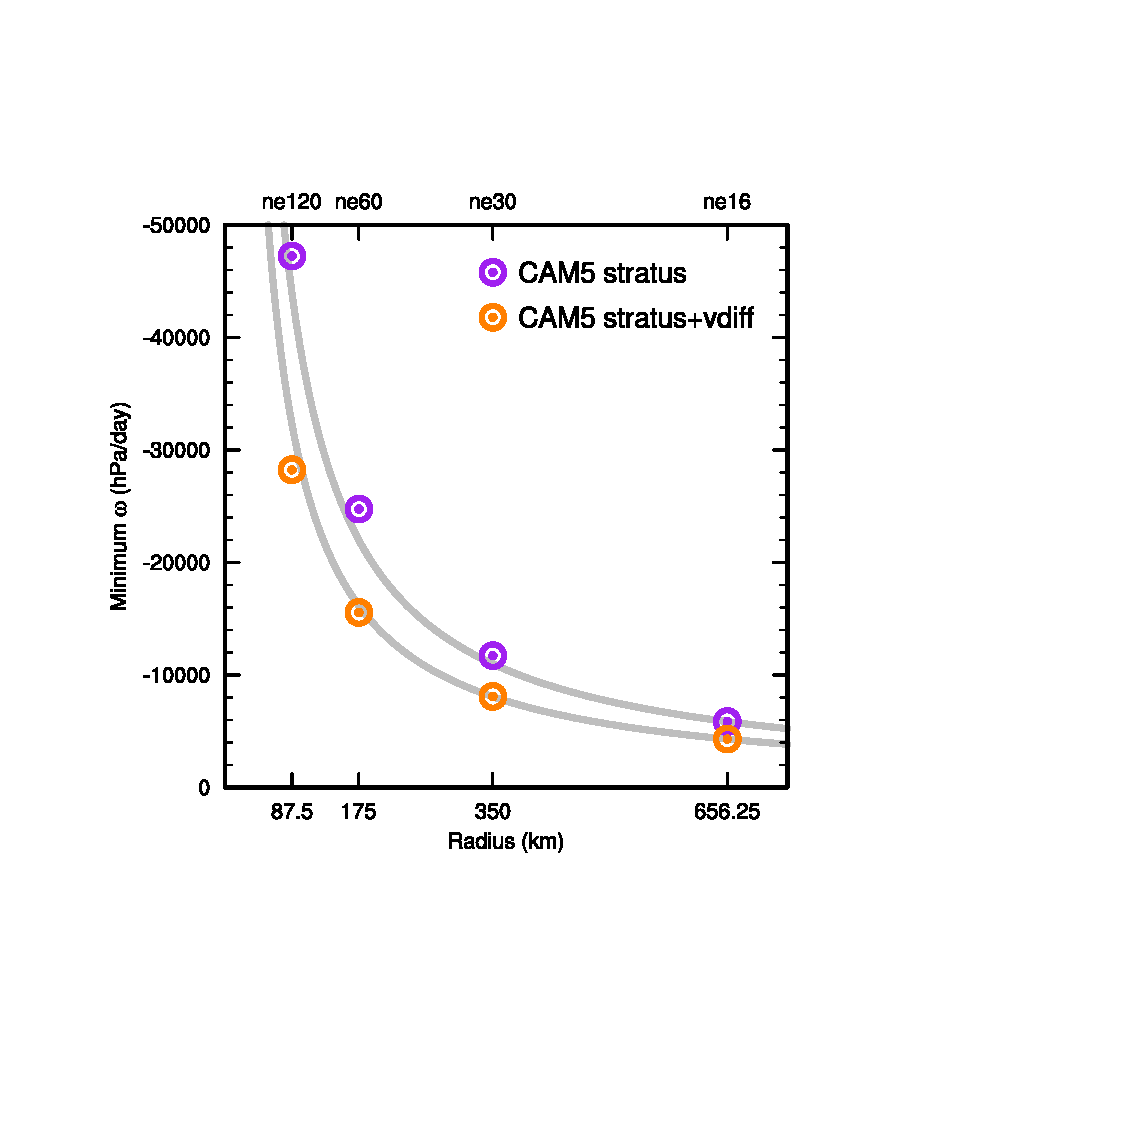
\includegraphics[width=20pc,angle=0]{chapter3/Figure5_crop.pdf}\\
\end{center}
\caption{As in Figure~\ref{fig:figure3-3}, but for the moist experiments using the CAM5 stratiform scheme (‘stratus’) and the CAM5 stratiform scheme coupled with the CAM5 vertical diffusion routine (‘stratus$+$vdiff’).}
\label{fig:figure3-5}
\end{figure}

\subsubsection{CAM-SE coupled to CAM5 Moist Physics}
The moist experiments are repeated using the more complex physics modules contained in the CAM5 physics package. Despite the increased complexity of the CAM5 stratiform cloud scheme (labeled as “stratus”) compared with the simple condensation scheme, the magnitudes of $\omega$ across the four different resolutions are nearly identical (Figures \ref{fig:figure3-5} and \ref{fig:figure3-3}). The inclusion of vertical dissipation (labeled as “stratus+vdiff”) reduces the magnitude of $\omega$ by about 40\%, but preserves the $1/r_h$ scaling (Figure~\ref{fig:figure3-5}). This is achieved through reducing the magnitude of the Archimedean buoyancy by local downgradient vertical mixing, but the scheme is unable to affect its horizontal scale. We conclude that the incorporation of moist processes, short of a convection scheme, maintains a physical response analogous to the physics of the dry system (equation~\ref{eq:eq3-3}).

\subsubsection{Sensitivity to physics time-step}
\paragraph{CAM-SE} ~\\
In all the moist experiments discussed so far, the physics time-step is set to 225 s. In practice, a longer physics time-step is used to minimize the computational overhead associated with the physics routines. For example, the default physics time-step in the ne30 configuration is 1800 s, and the experiments analyzed in \cite{HR2017JCLIM} use a physics time-step of 600 s. To explore the implications of using longer physics time-steps, the moist experiments are ran using physics time-steps of 450 s, 900 s and 1800 s. These experiments are performed using the simple condensation scheme and the CAM5 stratiform scheme.

\begin{figure}
\begin{center}
\noindent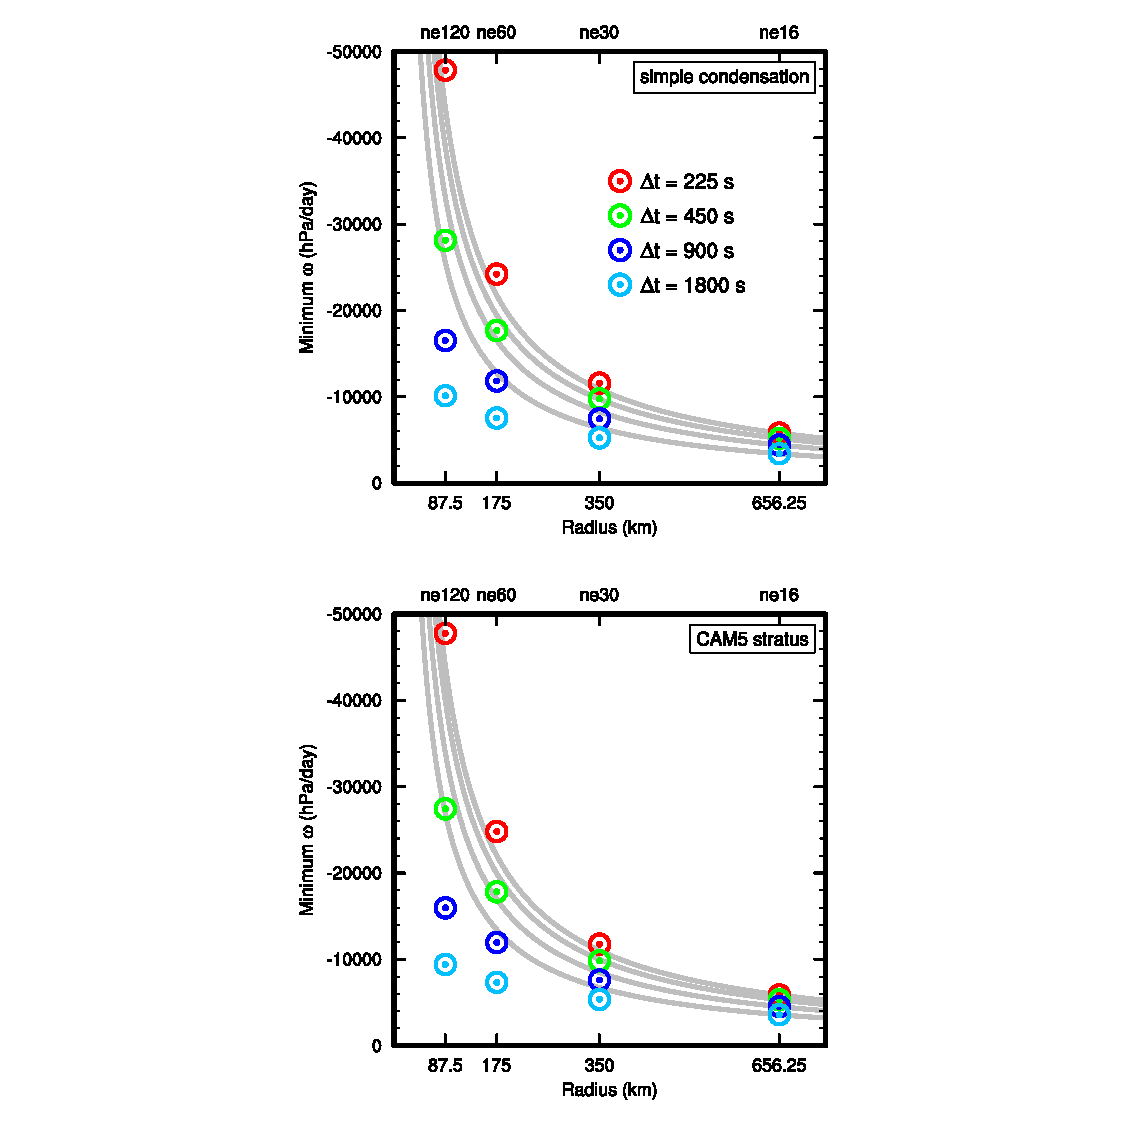
\includegraphics[width=20pc,angle=0]{chapter3/Figure6_crop.pdf}\\
\end{center}
\caption{As in Figure~\ref{fig:figure3-5}, but for the physics time-step sensitivity experiments using the simple condensation scheme (top) and the CAM5 stratiform scheme (bottom).}
\label{fig:figure3-6}
\end{figure}

The results of the physics time-step experiments for the two different condensation routines are shown in Figure~\ref{fig:figure3-6}. The time-step sensitivity using only the CAM5 stratus parameterization is almost identical to the time-step sensitivity of the simple condensation scheme (Figure~\ref{fig:figure3-6}). For a physics time-step of 450 s, the simulations begin to depart from the $1/r_h$ scaling observed in the 225 s experiments, damping the vertical motion at smaller $r_h$. At longer physics time-steps, the departure from $1/r_h$ scaling is even greater.

\paragraph{CAM-FV} ~\\
The time-step sensitivity experiment using the CAM5 stratiform routine has been repeated using the CAM-FV dynamical core (Figure~\ref{fig:figure3-7}). The magnitude of $\omega$ in CAM-FV is about 50\% less than in CAM-SE, at all resolutions (Figures \ref{fig:figure3-6} and \ref{fig:figure3-7}). This is consistent with simulations of tropical cyclones using these two dynamical cores – CAM-SE tends to have stronger storms as compared with CAM-FV \citep{RJ2012JAMES,RETAL2012ASL,RETAL2015JAS}. The qualitative behavior of the response to resolution and time-stepping is however, similar to CAM-SE – $\omega$ generally follow the scaling at small physics time-steps, but depart from the scaling at longer physics time-steps (Figure~\ref{fig:figure3-7}). Note that the $\omega$ field in the $2^{\circ}$ runs do not follow the scaling (not shown). To observe the scaling in CAM-FV at small physics time-steps, one must scale to a resolution other than $2^{\circ}$ (Figure~\ref{fig:figure3-7}).

\begin{figure}
\begin{center}
\noindent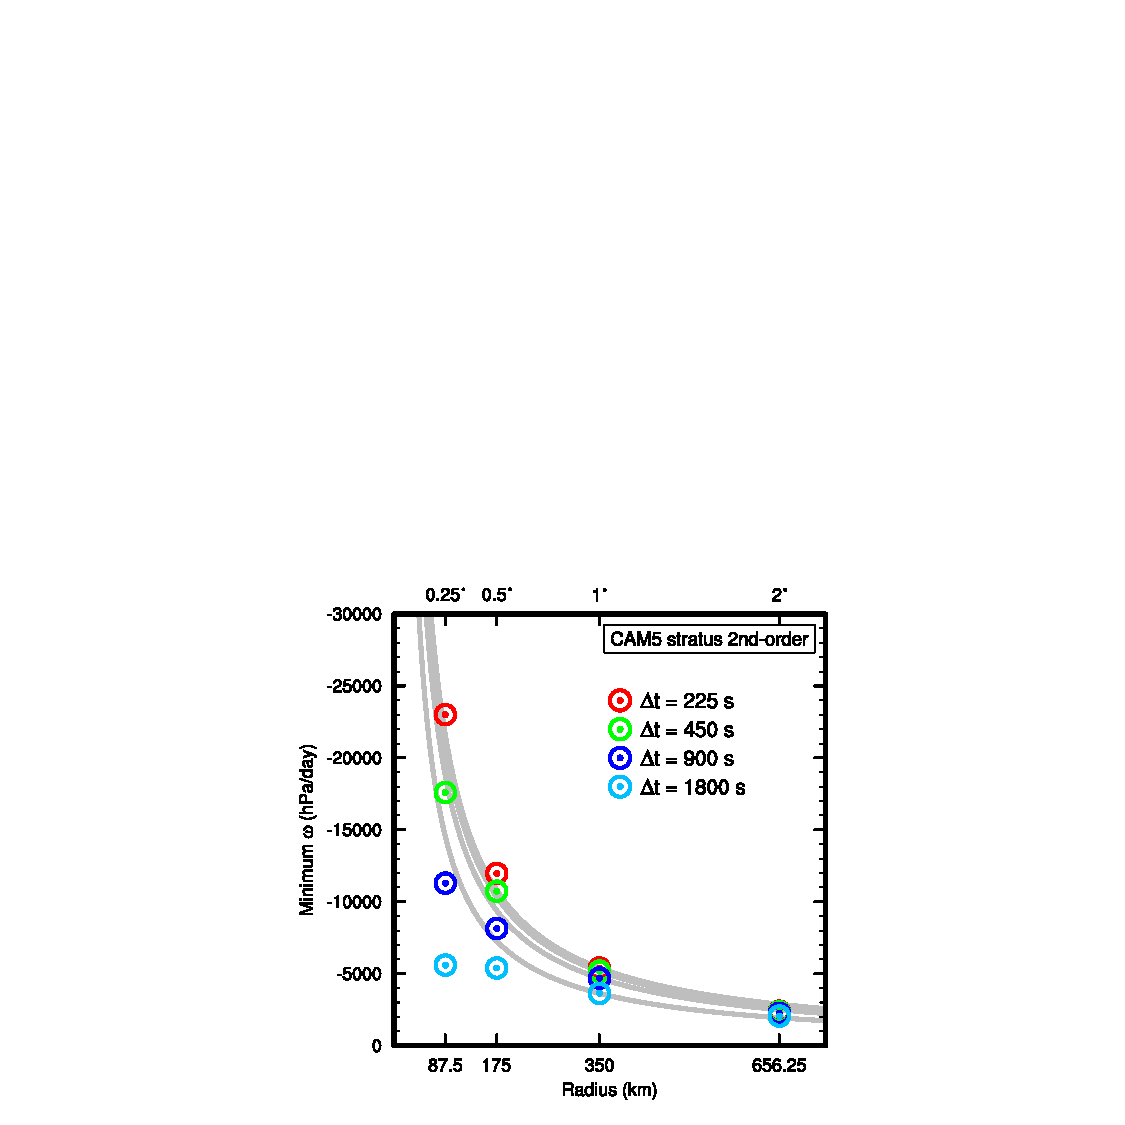
\includegraphics[width=20pc,angle=0]{chapter3/Figure7_crop.pdf}\\
\end{center}
\caption{As in Figure~\ref{fig:figure3-6}, but using the CAM-FV with second-order divergence damping. Note the analytical scaling (grey lines) have been scaled to the $1^{\circ}$ simulation in this plot, and the y-axis range in smaller, compared with Figure~\ref{fig:figure3-6}.}
\label{fig:figure3-7}
\end{figure}

The time-step sensitivity experiments in CAM-FV are repeated using the fourth-order divergence dampening operator, resulting in slightly lower magnitude vertical pressure velocities, but otherwise the experiment depicts a very similar sensitivity to physics time-step as the second order divergence damping simulation (not shown). The minimum $\omega$ in the simulation using the 225 s physics time-step and a $0.25^{\circ}$ grid, is -20179.8 hPa/day, compared to -23008.7 hPa/day with the second-order divergence damping. This result is intuitive – the higher the order of the divergence damping operator, the more effectively it damps near grid-scale features \citep{WJRL2010MWR}, such as the $\sim 7 \Delta x$ moist bubbles.

The fourth-order, internally computed divergence damping coefficient was found to be about twice as large as that used by CAM-SE. An additional simulation using the $0.25^{\circ}$ grid and 225 s time-step, in which the fourth-order divergence damping coefficient is lowered by an order of magnitude, results in an increase in the magnitude of $\omega$ by from -20179.8 hPa/day to -24689.7 hPa/day. The time-series of the minimum vertical pressure velocities in this simulation is compared to the equivalent CAM-SE simulation, in Figure~\ref{fig:figure3-8}, along with the CAM-FV simulation using the default fourth order divergence damping coefficient. While the larger divergence-damping coefficient used in CAM-FV may explain a portion of the differences between the CAM-SE and CAM-FV solutions, it does not explain most of the differences between the two solutions (Figure~\ref{fig:figure3-8}). The lower magnitude $\omega$ in CAM-FV may be a result of the diffusive nature of finite-volume numerics and/or limiters in the CAM-FV dynamical core \citep{LR1997QJR}, but could also be related to unphysical numerical aspects of the continuous Galerkin method, potentially resulting in artificially large magnitude  in CAM-SE. Further testing is required to provide conclusive evidence of the design aspects leading to the differences in solutions between these two dynamical cores.

\begin{figure}
\begin{center}
\noindent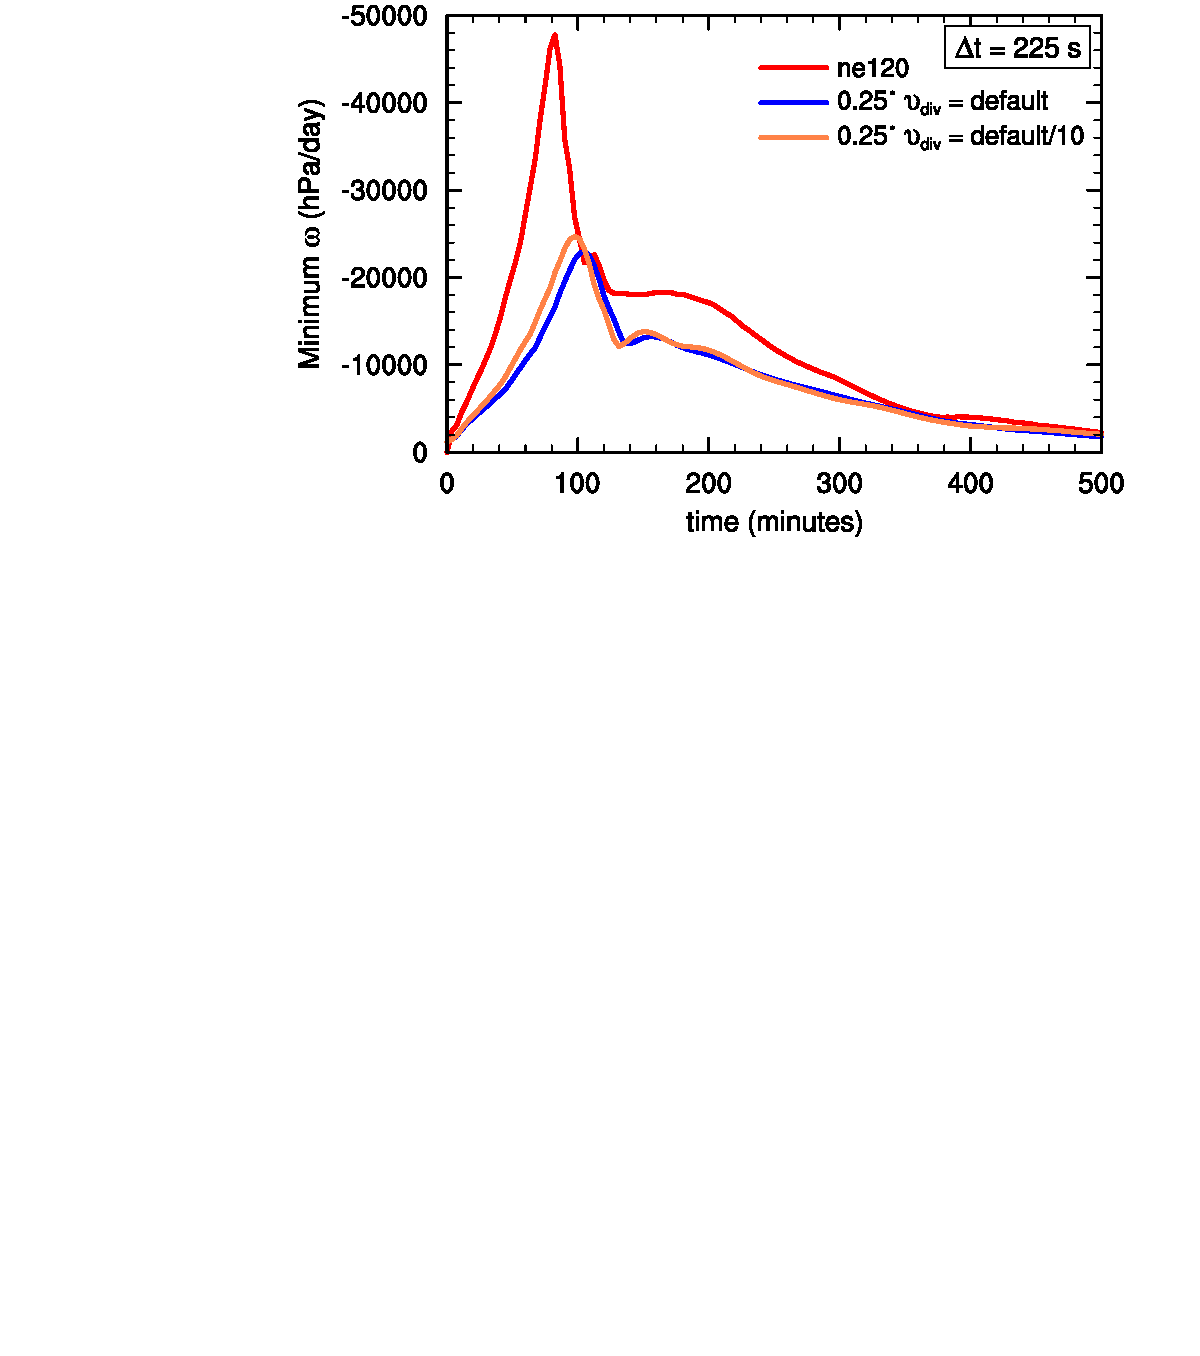
\includegraphics[width=25pc,angle=0]{chapter3/Figure8_crop.pdf}\\
\end{center}
\caption{Time-series of the minimum in $\omega$ for three different moist bubble simulations using the CAM5 stratiform scheme and a physics time-step of 225 s, at the highest grid resolution. The CAM-SE run is labeled `ne120’, while a pair of CAM-FV simulations using the fourth-order divergence damping are depicted, one using the default divergence damping coefficient, and another simulation with the coefficient reduced by an order of magnitude.}
\label{fig:figure3-8}
\end{figure}

\paragraph{Sensitivity to viscosity} ~\\
Through reducing the specific humidity hyper-viscosity coefficient in CAM-SE by an order of magnitude, the vertical velocity scaling is nearly recovered using a 450 s time-step (Supplementary Figure~\ref{fig:sfigure3-2}). Through individually reducing the hyper-viscosity coefficients on the other state variables (temperature, pressure thickness, non-divergent and divergent winds), the solutions either did not improve the scaling as effectively as the coefficient for specific humidity, or the model failed (note that the specific value of the coefficients are chosen by model developers, in part, for numerical stability). For example, model failure was common when reducing the divergence damping coefficient. In the simulations that did not crash, reducing the divergence damping coefficient by an order of magnitude lead to an increase in the magnitude of the vertical motion at all resolutions, but it’s effect on the scaling is ambiguous, and not as clear as the experiment in which specific humidity coefficient is reduced (Supplementary Figure~\ref{fig:sfigure3-2}).

\begin{figure}
\begin{center}
\noindent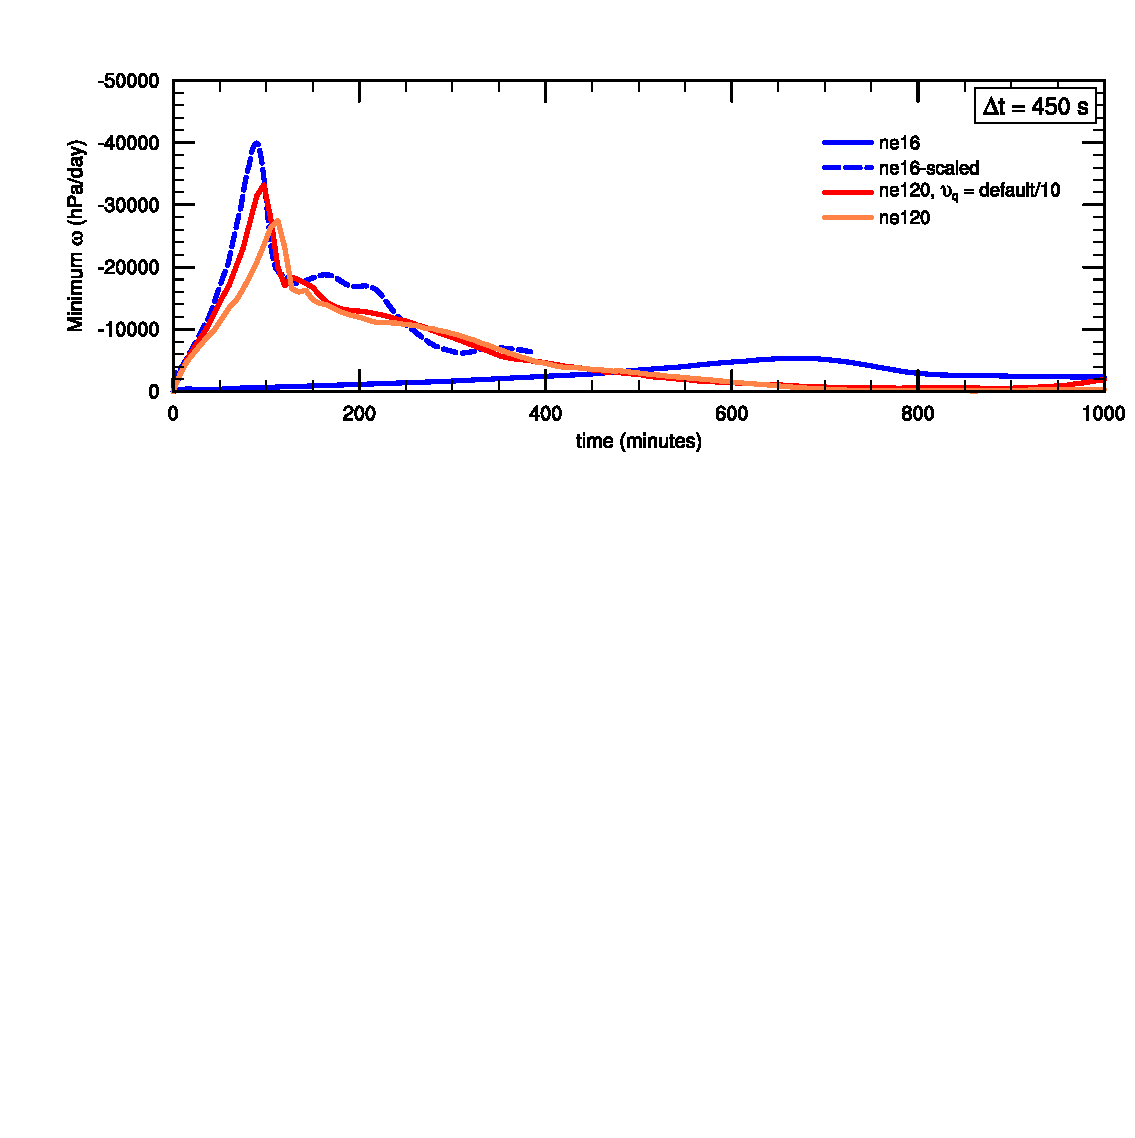
\includegraphics[width=35pc,angle=0]{chapter3/Figure9_crop.pdf}\\
\end{center}
\caption{Time-series of the minimum $\omega$ in three different CAM-SE moist bubble simulations using the CAM5 stratiform scheme and a physics time-step of 450 s. The dashed line shows the results of an ne16 simulation scaled to the ne120 resolution using equation~\ref{eq:eq3-3}. The orange line denotes the ne120 resolution simulation, while the red line is an ne120 simulation with the specific humidity hyper-viscosity coefficient reduced by an order of magnitude.}
\label{fig:figure3-9}
\end{figure}

Figure~\ref{fig:figure3-9} depicts the time dependence of the simulation in which the specific humidity hyper-viscosity coefficient is reduced by an order of magnitude. The results are presented as a time-series of the minimum $\omega$ in the highest resolution simulation, using a physics time-step of 450 s. The target solution, i.e., the solution found by scaling the lowest resolution simulation to the highest resolution using equation~\ref{eq:eq3-3}, as well as the highest resolution simulation using the default hyper-viscosity coefficients, are also shown in Figure~\ref{fig:figure3-9}. Through reducing the specific humidity coefficient, the ne120 solution approaches, but still underestimate, the target solution (Figure~\ref{fig:figure3-9}).

\subsection{Discussion}
The idealized experiments are evidence that the scaling of equation~\ref{eq:eq3-3} is maintained in a moist physics configuration, basically a two-component idealization of an AGCM containing only a dynamical core and large-scale condensation scheme, across multiple resolutions. Extending our results to the vertical velocity scaling observed in more complex configurations, such as aqua-planet experiments (e.g., Figure~\ref{fig:figure3-1}), may be a stretch. The CAM5 moist physics package contains shallow \citep{PB2009JC} and deep \citep{ZM1995AO,RR2008JC,NRJ2008JC} convection schemes. The large, predominantly stratiform thermals occurring only within the upper-troposphere in Figure~\ref{fig:figure3-1}, and the associated re-evaporation of falling condensate within the lower troposphere, are related to the deep convection scheme, and are designed to represent the effects of anvil cloud top formation in a deep convective system \citep{CAM5,PETAL2014JCLIM}. 

The source of moisture for the anvil tops in the model is primarily through detrainment of parameterized deep convective plumes, although moisture transport by the resolved dynamics and/or parameterized deep convective mass fluxes may be important as well. The anvil tops are confined to within the upper-troposphere because detrainment of the plume air is only permitted above the vertical level pertaining to the minimum in moist static energy \citep{ZM1995AO}. The deep convection scheme is designed to remove unstable air originating in the planetary boundary layer through vertical redistribution, severely limiting its ability to reduce the unstable conditions created through anvil cloud top formation. Therefore, to understand the model response to the rather popular anvil cloud tops (Figure~\ref{fig:figure3-1}), the reduced stratiform-dynamical core system may not be a terrible approximation. The initial conditions used in the idealized moist bubble experiments contain unstable conditions only above the planetary boundary layer, and a separate run using the complete CAM5 moist physics package confirms that the deep convection scheme is not triggered by the initial conditions (not shown).

It is not common for climate models to be ran using a physics time-step as small as 225 s, potentially explaining why the aqua-planet simulations of \cite{HR2017JCLIM} utilizing a 600 s physics time-step, or those discussed in the introduction using an 1800 s time-step (Figure~\ref{fig:figure3-10}, dashed lines), do not follow the vertical velocity scaling of equation~\ref{eq:eq3-3} across resolutions. To test this idea, four additional CAM-SE aqua-planet experiments are run, utilizing two different resolutions, ne30 and ne120. All four simulations are as described in the introduction, and are run for one year. The dynamics time-step was fixed between the two resolutions, set to 75 s, and each resolution is simulated twice using physics time-steps of 1800 s and then 225 s. The results of these four simulations are depicted in Figure~\ref{fig:figure3-10} as a probability density distribution of the negative $\omega$ at all vertical levels between $10^{\circ}$N and $10^{\circ}$S, computed from 6-hourly output over the final 11 months of the integration. The ne30 solutions are expressed as the ne30 probability density distribution scaled to the ne120 resolution following \cite{PG2006JAS},
\begin{equation}
P(\omega_1) = \alpha P(\omega_0 / \alpha), \label{eq:eq3-8}
\end{equation}
where $P(\omega)$ is the probability density distribution of the vertical pressure velocity, the subscripts refer to two different resolutions, $\Delta x_0$ and $\Delta x_1$, and $\alpha$ is the ratio of the velocity scale at $\Delta x_0$ to the velocity scale at $\Delta x_1$. Assuming the characteristic buoyancy of parcels in a simulation is unchanged between two resolutions, then through assuming $D \propto \Delta x$, $\alpha = \Delta x_1 / \Delta x_0$ from equation~\ref{eq:eq3-3}.

\begin{figure}
\begin{center}
\noindent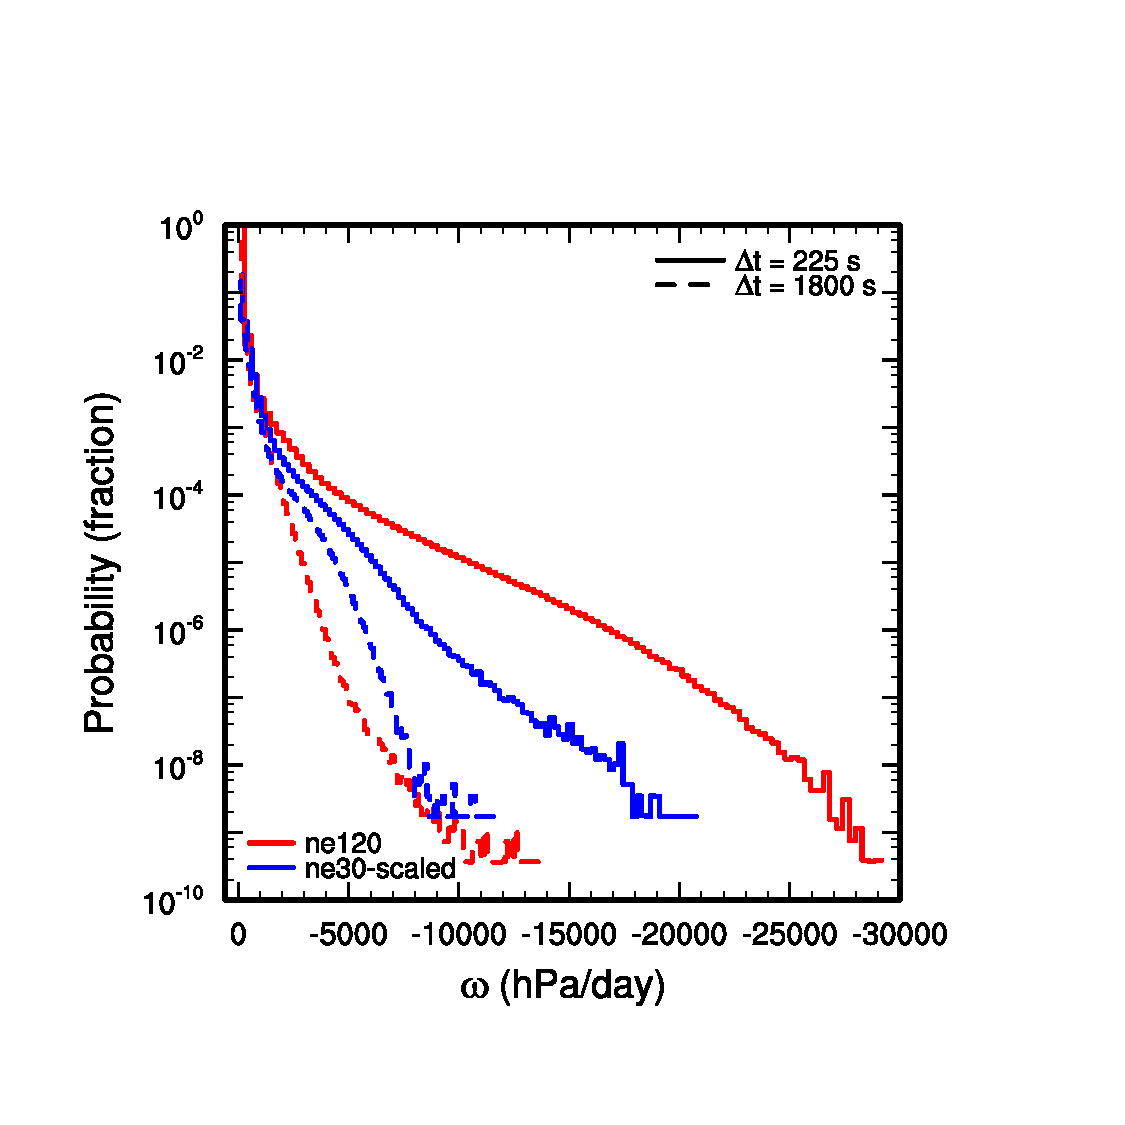
\includegraphics[width=20pc,angle=0]{chapter3/Figure10_crop.pdf}\\
\end{center}
\caption{Probability density distribution of negative  at all levels, and between $10{\circ}$N and $10^{\circ}$S, for four different aqua-planet simulations. An ne30 and ne120 simulation are depicted with colors, and the physics time-step used in the simulations are shown in different line styles. The ne30 solutions are expressed as ne30 solutions scaled to the ne120 resolution, as described in the text.}
\label{fig:figure3-10}
\end{figure}

Using an 1800 s physics time-step results in the usual scenario, with the scaled ne30 solutions generally over-predicting the occurrence of the ne120 upward  $\omega$ (Figure~\ref{fig:figure3-10}), although the mismatch is not as severe as in \cite{HR2017JCLIM}. This result is consistent with the moist bubble experiments - the over-prediction of vertical motion occurs using the 1800 s physics time-step (Figure~\ref{fig:figure3-6}). In contrast, with the 225 s physics time-step, the scaled ne30 solutions now under-predict the occurrence of large-magnitude vertical motion at high resolution (Figure~\ref{fig:figure3-10}), which does not occur in the moist bubble experiments (Figure~\ref{fig:figure3-6}). Reducing the physics time-step leads to larger magnitude vertical motions at both resolutions, which is apparent from the longer tails of the distributions (Figure~\ref{fig:figure3-10}). While the 225 s time-step simulations does not necessarily improve the ability of the scaling to explain the resolution sensitivity, the aqua-planet experiments are nonetheless consistent with idealized moist bubble experiments – the magnitude of the vertical motion is dampened through the use of longer physics time-steps, and more-so at higher resolution. 

One should bear in mind that comparing the relatively coarse time-sampling of the instantaneous $\omega$ in the aqua-planets (6-hourly) to the scaling derived from the high-frequency output (from 225 s to 1800 s) of the minimum $\omega$ in the moist bubble tests, may be reason alone for the observed difference in scaling between the two configurations. While the authors feel that the sampling bias is mitigated to some extent through the use of a large sample size to compute the aqua-planets statistics, concerns regarding dataset inconsistency have not been thoroughly explored.

The authors speculate that the mismatch between scaled and the actual solutions at short physics time-steps in the aqua-planets are due to a non-negligible change in thermodynamic properties of thermals across resolutions. One example leading to such a change is the occurrence of grid-point storms at high resolution and small physics time-steps, reported in \cite{W2013QJRMS}. Compared with the ne30 simulation, the response of the ne120 simulation to the shorter physics time-step leads to a proportionally larger increase in the magnitude of $\omega$ (Figure~\ref{fig:figure3-10}). The probability density distributions presented in \cite{W2013QJRMS} suggests that extreme values of $\omega$ in the tails of the distribution, such as occur in the ne120, 225 s time-step simulation (Figure~\ref{fig:figure3-10}), are consistent with grid-point storms. Grid-point storms can amplify $\omega$ through positive feedbacks on the parcel buoyancy, for example, by drawing in moisture through its own circulation, and over the course of the storms evolution \citep{W2013QJRMS}.

\subsection{Conclusions}
An idealized test was developed to understand the resolution sensitivity of the spectral-element (CAM-SE) and finite-volume (CAM-FV) dynamical core options of the Community Atmosphere Model, coupled with moist physics routines of varying complexity, and in the non-rotating limit. The test consists of analytical initial conditions of a buoyant bubble in a neutral environment, modeled after strongly convecting regions in aqua-planets. The bubble may be thought of as a surrogate cloud thermal arising from the physics package in more complex AGCM simulations. Through varying the planetary radius and holding the initial conditions fixed, the radius of the bubble ($r_h$) is reduced by the same factor as the planetary radius, approximating the reduction in diabatic forcing scale that occurs when increasing the horizontal resolution of an AGCM. The experiments were performed in a dry framework and a moist framework. In the dry experiments, the sensitivity of the vertical velocities to bubble radius is almost exactly proportional to $1/r_h$, consistent with the scale analysis of the Poisson equation (equation~\ref{eq:eq3-3}) adapted from \cite{JR2016QJRMS}.

Through including moisture, and a simple or more complex large-scale condensation routine, the $1/r_h$ scaling is maintained in both dynamical cores. This is by no means expected given that the analytical scaling is derived from the dry equations of motion, and indicates the potential usefulness of the moist bubble test for the intercomparison of dynamical cores \citep[e.g.,][]{RJ2012JAMES}. The greater available potential energy in the moist experiments results in vertical velocities that are an order of magnitude larger than in the dry experiments. In CAM-SE, incorporation of a downgradient vertical dissipation routine damps the Archimedean buoyancy and vertical velocity response, but still recovers the $1/r_h$ scaling. Experiments with the CAM-FV dynamical core simulate vertical pressure velocities about half as large, compared with CAM-SE. Sensitivity experiments indicate that the differences in the strength of the explicit divergence damping between these two dynamical cores probably can’t explain the main differences between the two models’ solutions.

While it is common for CAM to be ran using physics time-steps in the range of 600 s to 1800 s \citep{OETAL2013JCLIM,WETAL2014JAMES,RETAL2015JAS,ZetAl2014JCb,RM2016GRL}, we have used a smaller physics time-step of 225 s. Additional experiments using more conventional, larger physics time-steps results in a severely damped vertical velocity response to $r_h$, with more damping at larger time-steps. The specific mechanism leading to the time-truncation errors at large physics time-steps is difficult to determine exactly. One clue came from a separate CAM-SE experiment, in which the scaling was nearly recovered with the hyper-viscosity coefficient for specific humidity dissipation reduced by an order of magnitude. We speculate that numerical dissipation from the dynamical core may result in time-truncation errors when the ratio of the physics to dynamics time-step is too large, resulting in too infrequent coupling between two fast processes, the condensation routine with its near instantaneous release of available potential energy, and the convectively unstable dynamics.

It is difficult to make an argument for or against a smaller physics time-step from this study alone. Due to our choice of horizontal resolution in this study, ‘thermals’ are represented as laminar, rising bubbles of hydrostatic scale. At cloud resolving scales, thermals are characterized as highly turbulent \citep{GETAL1991JAS,WS1998MWR,BETAL2002MWR}, consisting of $O$(100 m) turbulent eddies that mix the cloud and environment. \cite{TETAL2017JAMES} have illustrated the importance of the sub-grid turbulence scheme at cloud permitting resolutions, exerting strong control over moisture entrainment, the thermodynamic properties of convecting cores and large-scale organization. While a numerical filter should not be confused as a turbulence closure \citep{JW2010LNCSE}, unless, perhaps if it is explicitly designed for that purpose \citep[e.g.,][]{GMR2007,METAL2015JCP}, there is certainly the possibility that modulating the strength of the numerical filter might act as some form of entrainment parameter for the grid-scale thermals in AGCM simulations. On the other hand, it has been argued that AGCMs are overly-dissipative \citep{S2005QJR,BETAL2012JCLIM}, implying that additional damping resulting from a longer physics time-step is not preferred. In any case, it is instructive for model users to understand that there is a large sensitivity of the vertical motion to physics time-step, especially at high resolution.

It may not be worth dismissing the relevance of this work to more complex AGCM configurations entirely due to the omission of convection schemes. Large, positive buoyancy forcing from the stratiform scheme frequently occurs above the planetary boundary layer, limiting a convection schemes ability to respond to this instability. The results of the aqua-planet experiments, which utilize the complete CAM5 physics package, generally support the notion of time-truncation errors at large physics time-step uncovered in the moist bubble experiments, suggesting there may be utility in studying the behavior of the reduced large-scale condensation-dynamical core system. This is not to suggest that the convection schemes and stratiform scheme are entirely decoupled from one another - the convection schemes are crucial for pumping heat and moisture out of the boundary layer, often providing the near-saturated conditions in the free-troposphere that is eventually condensed by the stratiform scheme \citep{PETAL2014JCLIM}. Future efforts will work towards initializing the boundary layer with unstable conditions in order to understand the influence of convection schemes on the vertical velocity scaling. 

Finally, our work has implications for understanding the resolution sensitivity of AGCMs. This study, along with \cite{HR2017JCLIM}, have shown that by assuming a linear relation between the horizontal scale of the diabatic forcing and the grid spacing, the analytical scaling derived from the dry equations of motion over-estimates the vertical velocity response to horizontal resolution in aqua-planet simulations, using conventional long physics time-steps. Through reducing the physics time-step to a less conventional 225 s, the problem appears to be reversed: the scaled solutions under-predict the magnitude of the vertical motion of the aqua-planets across resolutions. The authors speculate that this under-prediction is related to a change in characteristic parcel buoyancy across resolutions, e.g., due to the occurrence of grid-point storms at high resolution and short physics time-steps, identified in a prior version of CAM \citep{W2013QJRMS}. Additionally, the relationship between forcing scale and grid spacing may be non-linear, for example, if the forcing scale is determined by emergent constraints on the spectral properties of mesoscale circulations \citep{RETAL2016CD,OETAL2016JAMES}. 

While there may be other factors contributing to the resolution sensitivity of the aqua-planets \citep[e.g.,][]{LETAL2015JCLIM}, our idealized experiments has made clear that the vertical velocity across different resolutions is to first-order determined by the inverse of the forcing scale, and that departures from that scaling can occur through feedbacks with other components of the model. Rather than laying the burden of resolution sensitivity entirely on the moist physical parameterizations, this work is consistent with the idea that the inherent scale dependencies of the dynamical core are instead instigated by the horizontal scale of the buoyancy forcing the grid is able to support. The implications of the latter are that resolved updrafts and downdrafts, which are perhaps more wide-spread in AGCMs than previously thought, are very sensitive to horizontal resolution.

\begin{figure}
\begin{center}
\noindent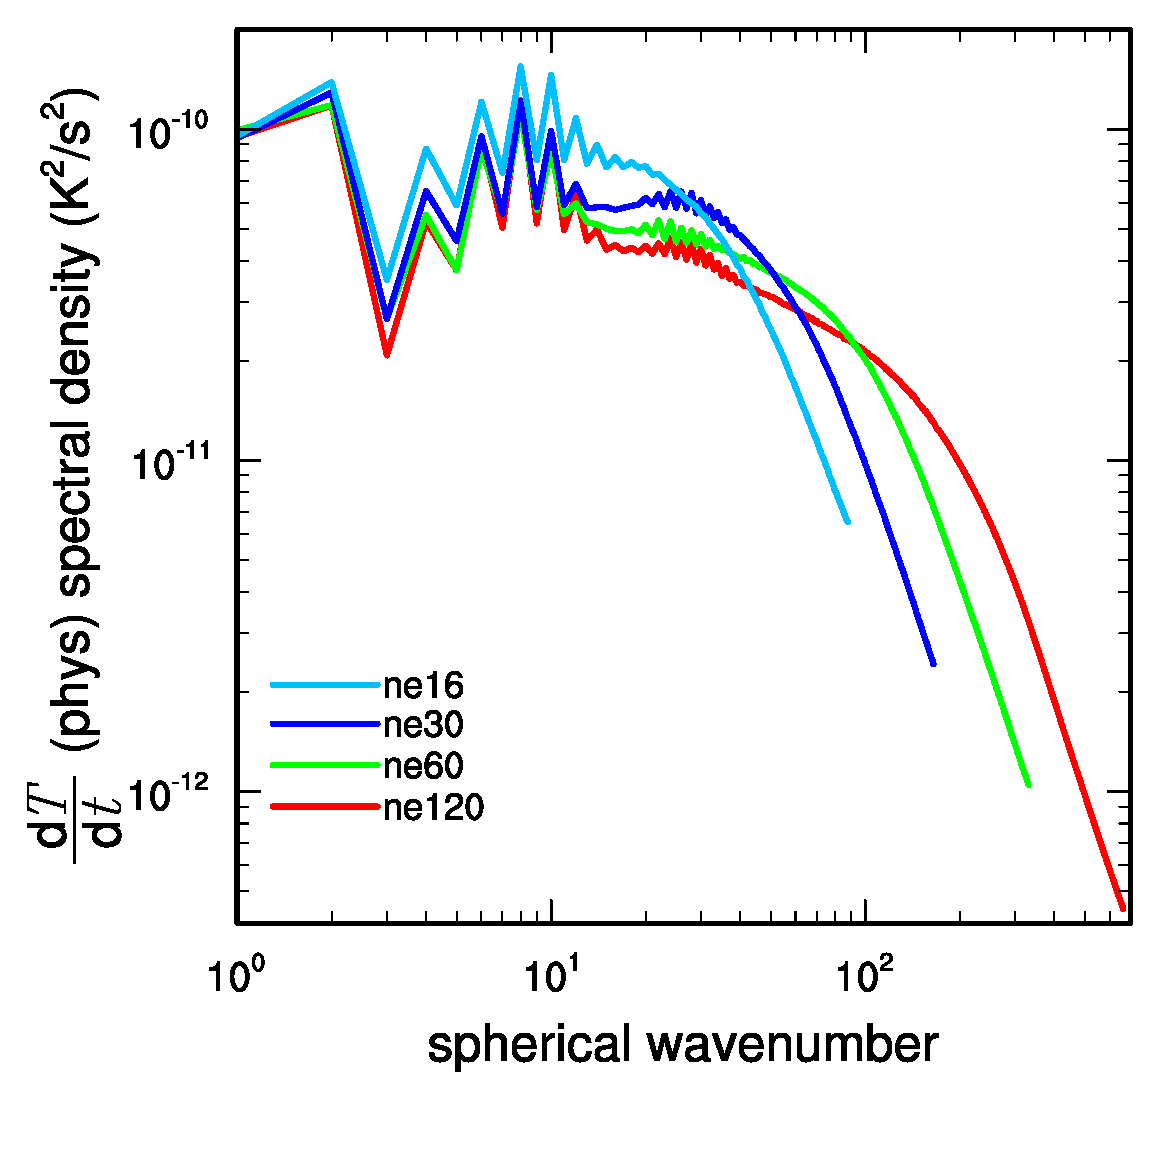
\includegraphics[width=25pc,angle=0]{chapter3/SFigure1.eps}\\
\end{center}
\caption{Global 400 hPa power spectral density of the temperature tendency arising from the CAM5 physics routines in the aqua-planet simulations.}
\label{fig:sfigure3-1}
\end{figure}

\begin{figure}
\begin{center}
\noindent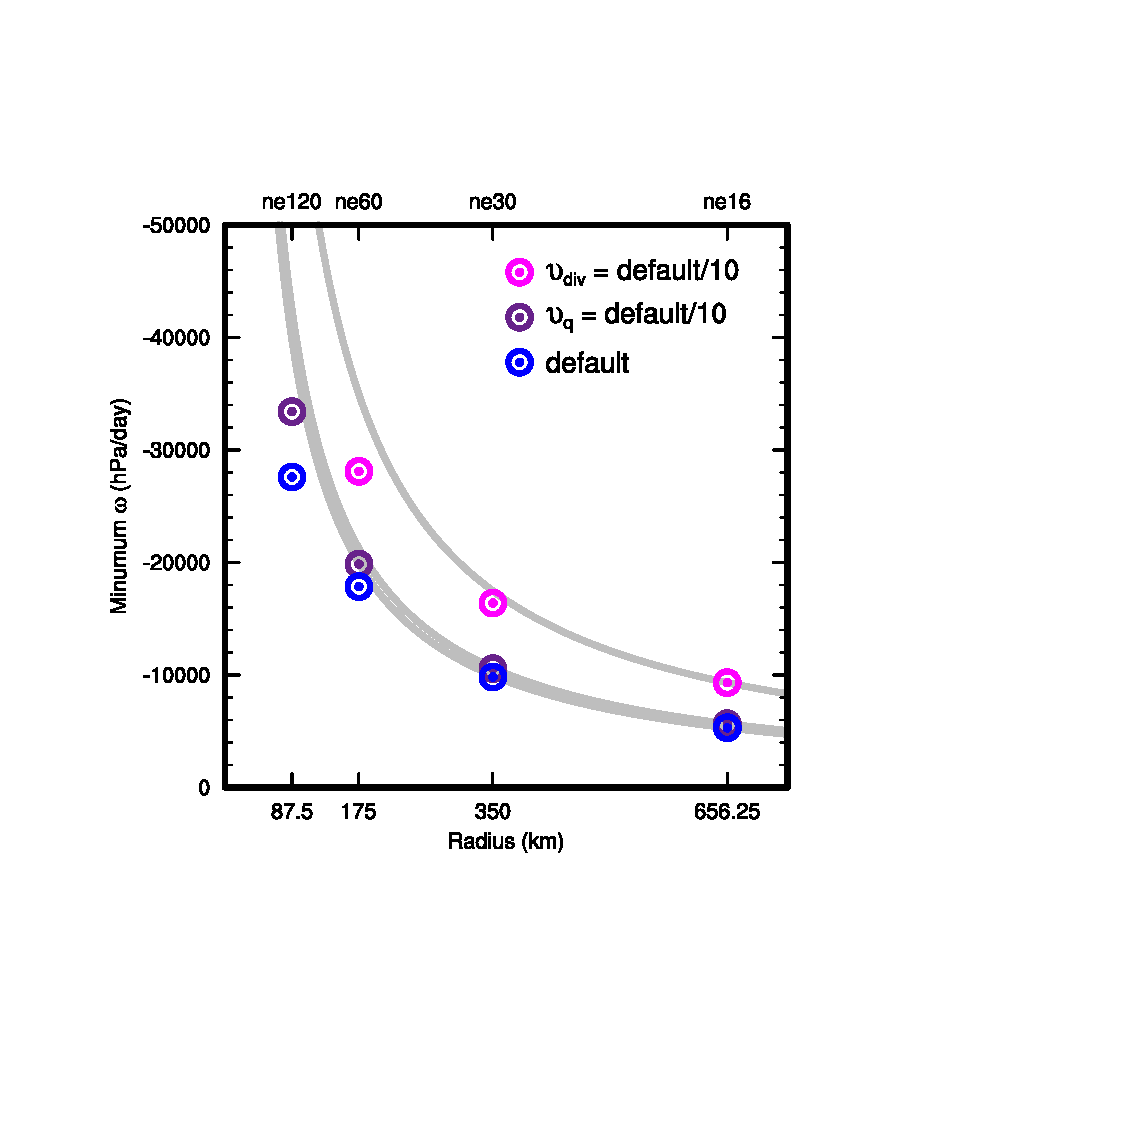
\includegraphics[width=25pc,angle=0]{chapter3/SFigure2_crop.pdf}\\
\end{center}
\caption{Results of three moist bubble experiments using CAM-SE coupled to the CAM5 stratiform scheme, using a physics time-step of 450 s. Results are expressed as the minimum vertical pressure velocity, $\omega$, over the duration of each simulation as a function of initial bubble radius. Each experiment contains four simulations, with grid-spacing (top x-axis) and initial size of the bubble (bottom x-axis) progressively decreasing. The purple markers indicate an experiment in which the specific humidity hyper-viscosity coefficient is reduced by an order of magnitude. Similarly, the pink markers denote an experiment in which the divergence damping coefficient is reduced by an order of magnitude. The highest resolution divergence damping coefficient result is not shown since this configuration resulted in model failure.}
\label{fig:sfigure3-2}
\end{figure}
 \label{sec:chapter3}

\newpage
\begin{center}
\section{Physics-dynamics coupling with element-based high-order Galerkin methods: quasi equal-area physics grid}
%\chapter{\bf{\normalsize Physics-dynamics coupling with element-based high-order Galerkin methods: quasi equal-area physics grid}}
\end{center}
%\addcontentsline{toc}{section}{\protect\numberline{}Physics-dynamics coupling with element-based high-order Galerkin methods: quasi equal-area physics grid}
%\addcontentsline{toc}{chapter}{\protect\numberline{}Physics-dynamics coupling with element-based high-order Galerkin methods: quasi equal-area physics grid}
\subsection{Introduction}
An increasing number of numerical methods publications in the atmospheric science literature concern transport, shallow-water, and three-dimensional models employing element-based high-order Galerkin discretizations such as finite-element and discontinuous Galerkin methods \citep[for an introduction to these methods see, e.g., ][]{Durran,NLL2011LNCSE,U2014GMD}. Some global models based on Galerkin methods have reached a level of maturity for which they are being considered for next generation climate and weather models due to their inherent conservation properties, high-order accuracy (for smooth problems), high parallel efficiency, high processor efficiency, and geometric flexibility facilitating mesh-refinement applications. NCAR's Community Atmosphere Model \citep[CAM; ][]{CAM5} offers a dynamical core based on continuous Galerkin finite elements \citep{TF2010JCP}, referred to as CAM-SE \citep[CAM Spectral Elements; ][]{TES2008JPCS,DetAl2012IJHPCA,LetAl2018JAMES}. CAM-SE is, in particular, being used for high resolution climate modeling \citep[e.g., ][]{JAME:JAME20125,RetAl2015GRL,BETAL2018CC} and static mesh-refinement applications \citep[e.g., ][]{FT2004MWR,ZetAl2014JC,ZetAl2014JCb,GetAl2014GMD,RHUZ2016JAMC}. Other examples of models based on high-order Galerkin methods that are being considered for `operational' weather-climate applications are \citet{Giraldo20083849}, \citet{NCT2009CF}, \citet{BSBDK2013TCFD} and the Energy Exascale Earth System Model (\url{https://e3sm.org/}).

\begin{figure}[t]
\begin{center}
\noindent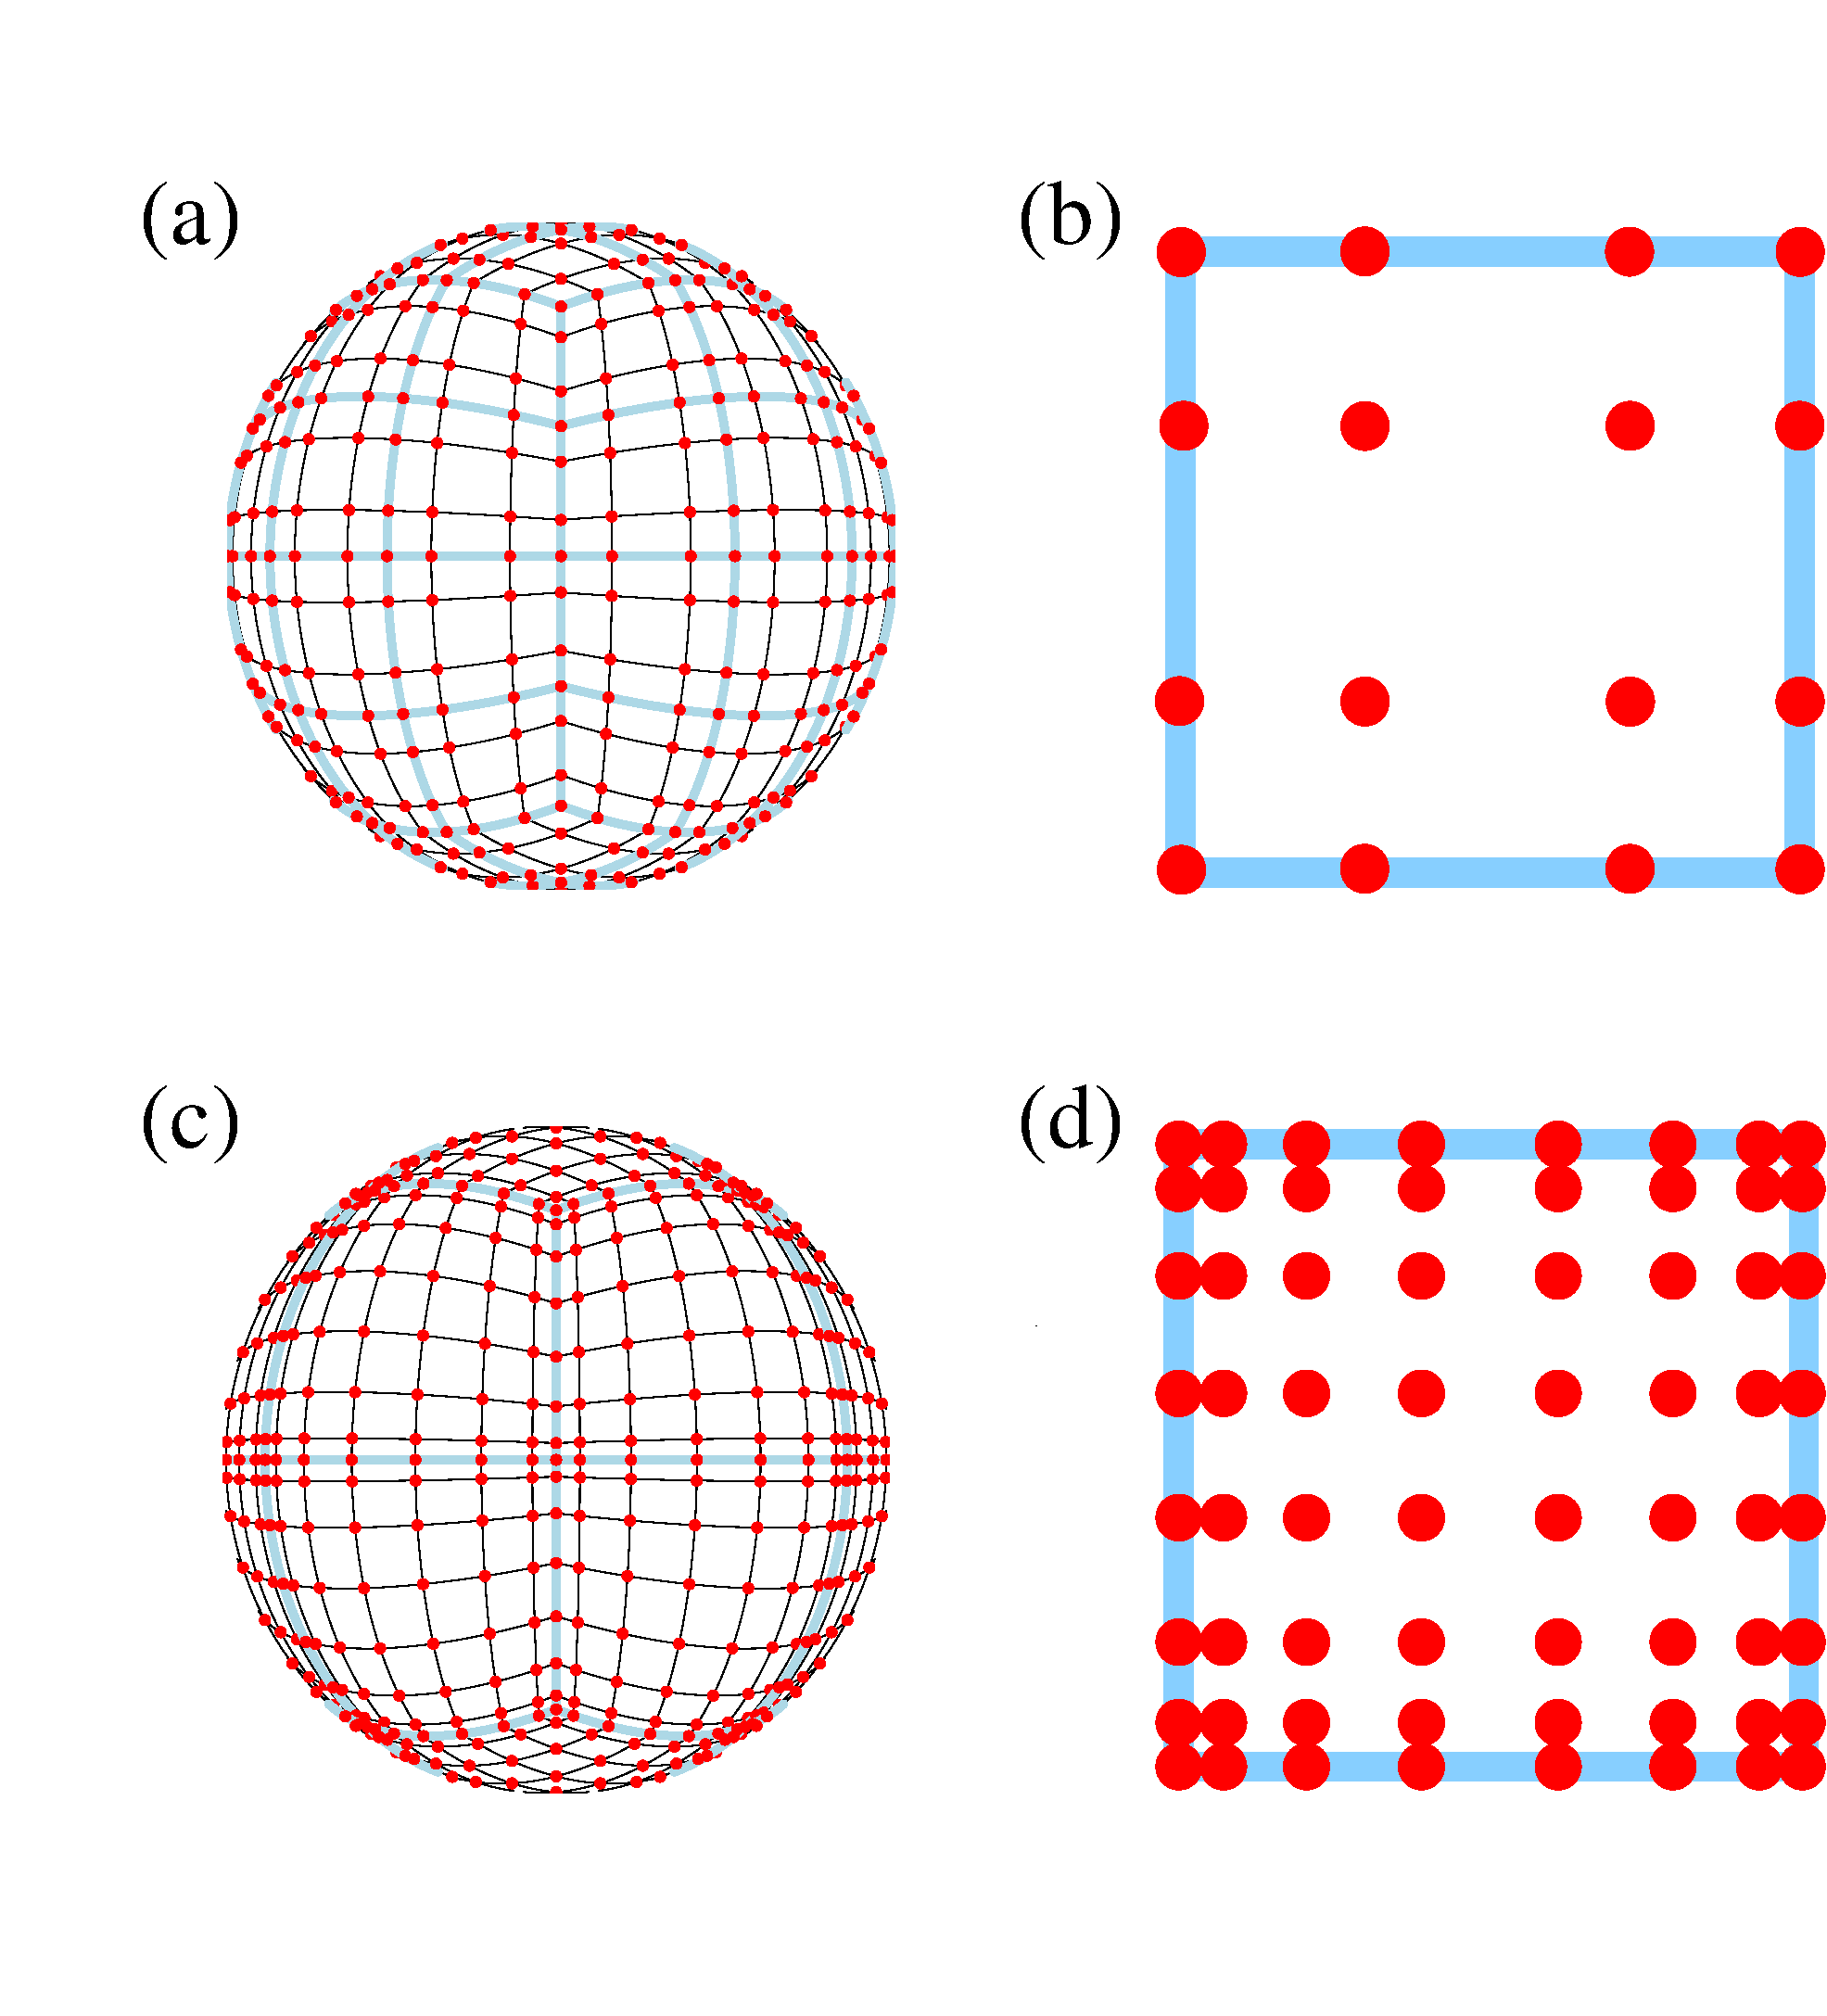
\includegraphics[width=25pc,angle=0]{chapter4/gll.pdf}\\
\end{center}
\noindent
\caption{Example of CAM-SE GLL quadrature grids, marked with red filled circles, (a \& c) on the cubed-sphere and (b \& d) in an element. (a)-(b) and (c)-(d) use $4\times 4$ ($np=4$) and $8\times 8$ ($np=8$) GLL quadrature points in each element, respectively. (a) and (c) have the same average grid-spacing at the Equator (7.5$^\circ$) which is obtained by using (a) $4\times 4$ ($ne=4$) and (b) $2\times 2$ ($ne=2$) elements on each cubed-sphere face/panel, respectively. The element boundaries are marked with thick light blue lines. The grid configurations shown on (a) and (c) are referred to as $ne4np4$ and $ne2np8$, respectively.}
\label{fig:gll-grids}
\end{figure}

Assumptions inherent to the physical parameterizations (also referred to as {\em{physics}}) require the state passed by the dynamical core represent a `large-scale state', for example, in quasi-equilibrium-type convection schemes \citep{AS1974JAS,PC2008JAS}. In finite-volume methods \citep[e.g., ][]{L2004MWR}, one may think of the dynamical core state as the average state of the atmosphere over a control volume, and for resolutions typical of climate simulations is entirely consistent with the notion of a `large-scale state'. For finite-difference methods \citep[e.g., ][]{SETAL983MWR} the point value is thought of as representative for the atmospheric state in the vicinity of the point value and one can usually associate a volume with the grid-point. Hence the physics grid (the grid on which the state of the atmosphere is evaluated and passed to physics) and the dynamics grid (the grid the dynamical core uses) coincide. Having the physics and dynamics grids coincide is obviously convenient since no interpolation is needed (which could disrupt conservation properties) and the number of degrees of freedom on both grids is exactly the same. 

For the regular latitude-longitude, cubed-sphere and icosahedral grids the distance between the grid-points is gradually varying for finite-volume/finite-difference discretizations. Examples of models that use these grids are CAM-FV \citep[latitude-longitude grid, ][]{L2004MWR}, FV3 \citep[cubed-sphere grid, ][]{PL2007JCP} and ICON \citep[icosahedral grid, ][]{WETAL2013GMD}. For high-order element-based Galerkin methods, the dynamical core grid is defined by the quadrature points. In CAM-SE, these are the Gauss-Lobatto-Legendre (GLL) quadrature nodes. A unique aspect of the high-order quadrature rules is that the nodes within an element are located at the roots of the basis set, which may be irregularly spaced. For example, Figure \ref{fig:gll-grids} shows GLL points on an individual element of a cubed-sphere grid for degree 3 ($np\times np=4\times 4$ quadrature points) and degree 7 ($np\times np=8\times 8$ quadrature points) Lagrange polynomial basis used in CAM-SE. The higher the order of the quadrature rule, the greater variance in distance between GLL quadrature points within an element. GLL quadrature points cluster near the edges and, in particular, the corners of the elements.

The resolved scales of motion are not determined by the distance between quadrature nodes, but rather the degree of the polynomial basis in each element. The nodes may be viewed as irregularly spaced samples of an underlying spectrally truncated state. From this perspective, one might expect the nodal solutions to be independent of location within an element. While the interior quadrature nodes are $C^{\infty}$ in CAM-SE (i.e. the basis representation is infinitely smooth and all derivatives are continuous), the smoothness of boundary nodes are constrained by the need to patch neighboring solutions together to form the global basis set, an operation known as the direct stiffness summation \citep[DSS; ][]{MadayPatera87,canuto2007}. The DSS operation is attractive because it allows for high-order accuracy with minimal communication between elements, but degrades the solution to $C^0$ at element boundaries (i.e., all derivatives are discontinuous). Through evaluating the physics at the nodal points, strong grid-scale forcing or oscillatory behavior near an element boundary may exacerbate the discontinuity, and our initial expectation, that the nodal solutions are independent of within-element location, is unlikely for non-smooth problems, e.g., the presence of rough topography or moist physics grid-scale forcing.

It is the purpose of this paper to document the implementation of an entirely separate, quasi-equal area finite-volume physics grid into CAM-SE. The use of a separate physics grid is not entirely unheard of; prior studies have utilized the infrastructure developed for global-spectral transform methods to experiment with different physics grids \citep{W1999T,W2014PTRSL}. In our framework, the dynamical core state is integrated over control volumes to provide a volume averaged state to the physics, thereby minimizing the influence of any one particular nodal value on the physics forcing. Section \ref{sec:nodeproblem} provides a thorough explanation of how grid imprinting manifests in high-order Galerkin methods for non-smooth problems. The implementation of the physics grid configuration into CAM-SE is presented in Section \ref{sec:methods4}. Results from a hierarchy of idealized model configurations are presented in Section \ref{sec:results4}, illustrating the physics grid is effective at mitigating undesirable grid imprinting in the solution. Section \ref{sec:conclusions4} contains a discussion of results and concluding remarks.

\subsection{The Quadrature Node Problem}\label{sec:nodeproblem}

Figure~\ref{fig:se-schematic} is a schematic illustrating in one-dimension how grid-imprinting is enabled by the physics, when the dynamical core is built using high-order Galerkin methods. The schematic depicts a time-step, starting from smooth initial conditions (Figure~\ref{fig:se-schematic}a), and subsequently advancing the dynamics one Runge-Kutta time-step (Figure~\ref{fig:se-schematic}b). Since the boundary nodes of adjacent elements overlap one-another, there are now two solutions for each boundary node. The DSS operator, effectively a numerical flux applied to the element boundaries such that overlapping nodal values agree, is applied (Figure~\ref{fig:se-schematic}c), rendering the solutions at element boundaries $C^0$; less-smooth than neighboring $C^{\infty}$ interior nodes. An element boundary discontinuity may be exacerbated if, e.g., the physics updates the state at an element boundary (Figure~\ref{fig:se-schematic}d,e), resulting in characteristically tighter gradients on the boundary nodes compared to if the physics forcing were applied to an interior node (Figure~\ref{fig:se-schematic}g,h).   

\begin{figure}[t]
\begin{center}
\noindent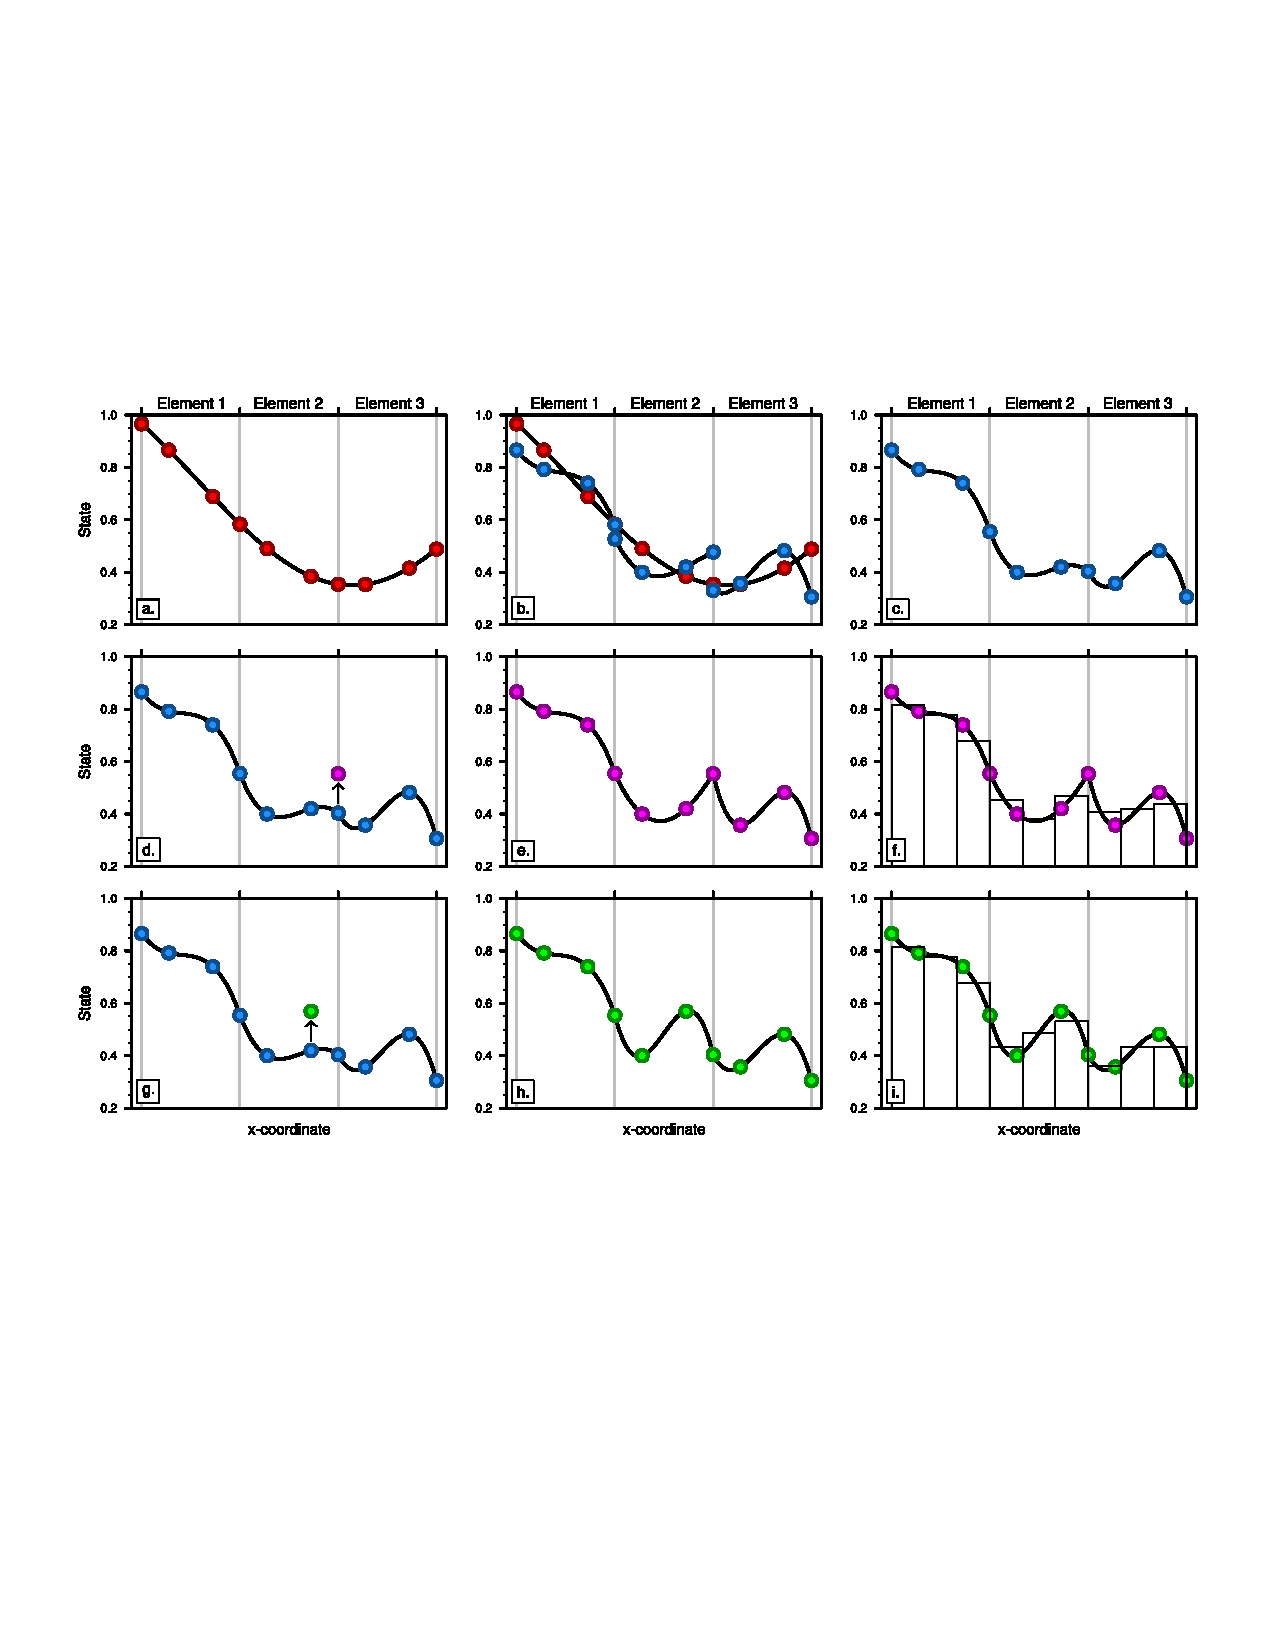
\includegraphics[width=35pc,angle=0]{chapter4/se-schematic-arh-CROP.pdf}\\
\end{center}
\caption{A one-dimensional schematic showing the relationship between the basis functions, the quadrature nodes and the proposed physics grid, over the coarse of a time-step. The filled circles are the GLL quadrature points in each element, which are connected by a Lagrange polynomials basis (curves). (a) Smooth initial condition are (b) advanced by the dynamics one Runge-Kutta step (blue), and (c) shows the solution after applying the DSS operator. Applying (d) grid-scale forcing to an element boundary node, (e) the basis representation is clearly $C^0$ at the element boundary. In contrast, (d) applying grid-scale forcing to an interior node (e) results in a smooth, $C^{\infty}$ continuous field. (f),(i) Vertical bars pertain to the values on the physics grid, found through integrating the basis functions over the control volumes.}
\label{fig:se-schematic}
\end{figure}

To test the degree to which nodal solutions depend on within-element position, an aqua-planet simulation \citep{NH2000ASL,MWO2016JAMES}, which consists of an ocean covered planet in perpetual equinox, with fixed, zonally symmetric sea surface temperatures idealized after the present day climatology, is carried out using CAM-SE, using CAM, version 4 physics \citep[CAM4;][]{CAM4} and run for one year. The nominal low resolution $ne30np4$ grid is used, pertaining to an average equatorial grid spacing of $111.2km$. The probability density distribution of the upward vertical pressure velocity ($\omega$), conditionally sampled based on three categories - `interior', `edge' and `corner' nodes - is provided in Figure~\ref{fig:omega-se-volumes}a. The motivation for assessing noise in the $\omega$ field comes from its connection with the atmosphere's divergent modes, as follows from the continuity equation in pressure coordinates. These modes are in turn sensitive to the within-element inhomogeneity of the pressure gradient that emerges from high-order Galerkin methods. There is an apparent dependence on nodal location, with interior nodes being characteristically sluggish, and corner and edge nodes having systematically larger magnitude vertical motion. This behavior is consistent with the smoothness properties of the different nodal locations, with discontinuous pressure gradients resulting in greater vertical motion at edge and corner nodes. The main division of solutions shown in Figure~\ref{fig:omega-se-volumes}a is primarily between whether a node is, or is not situated on an element boundary, and is a nuanced signature of high-order element-based Galerkin methods for non-smooth problems.

\begin{figure}[t]
\begin{center}
\noindent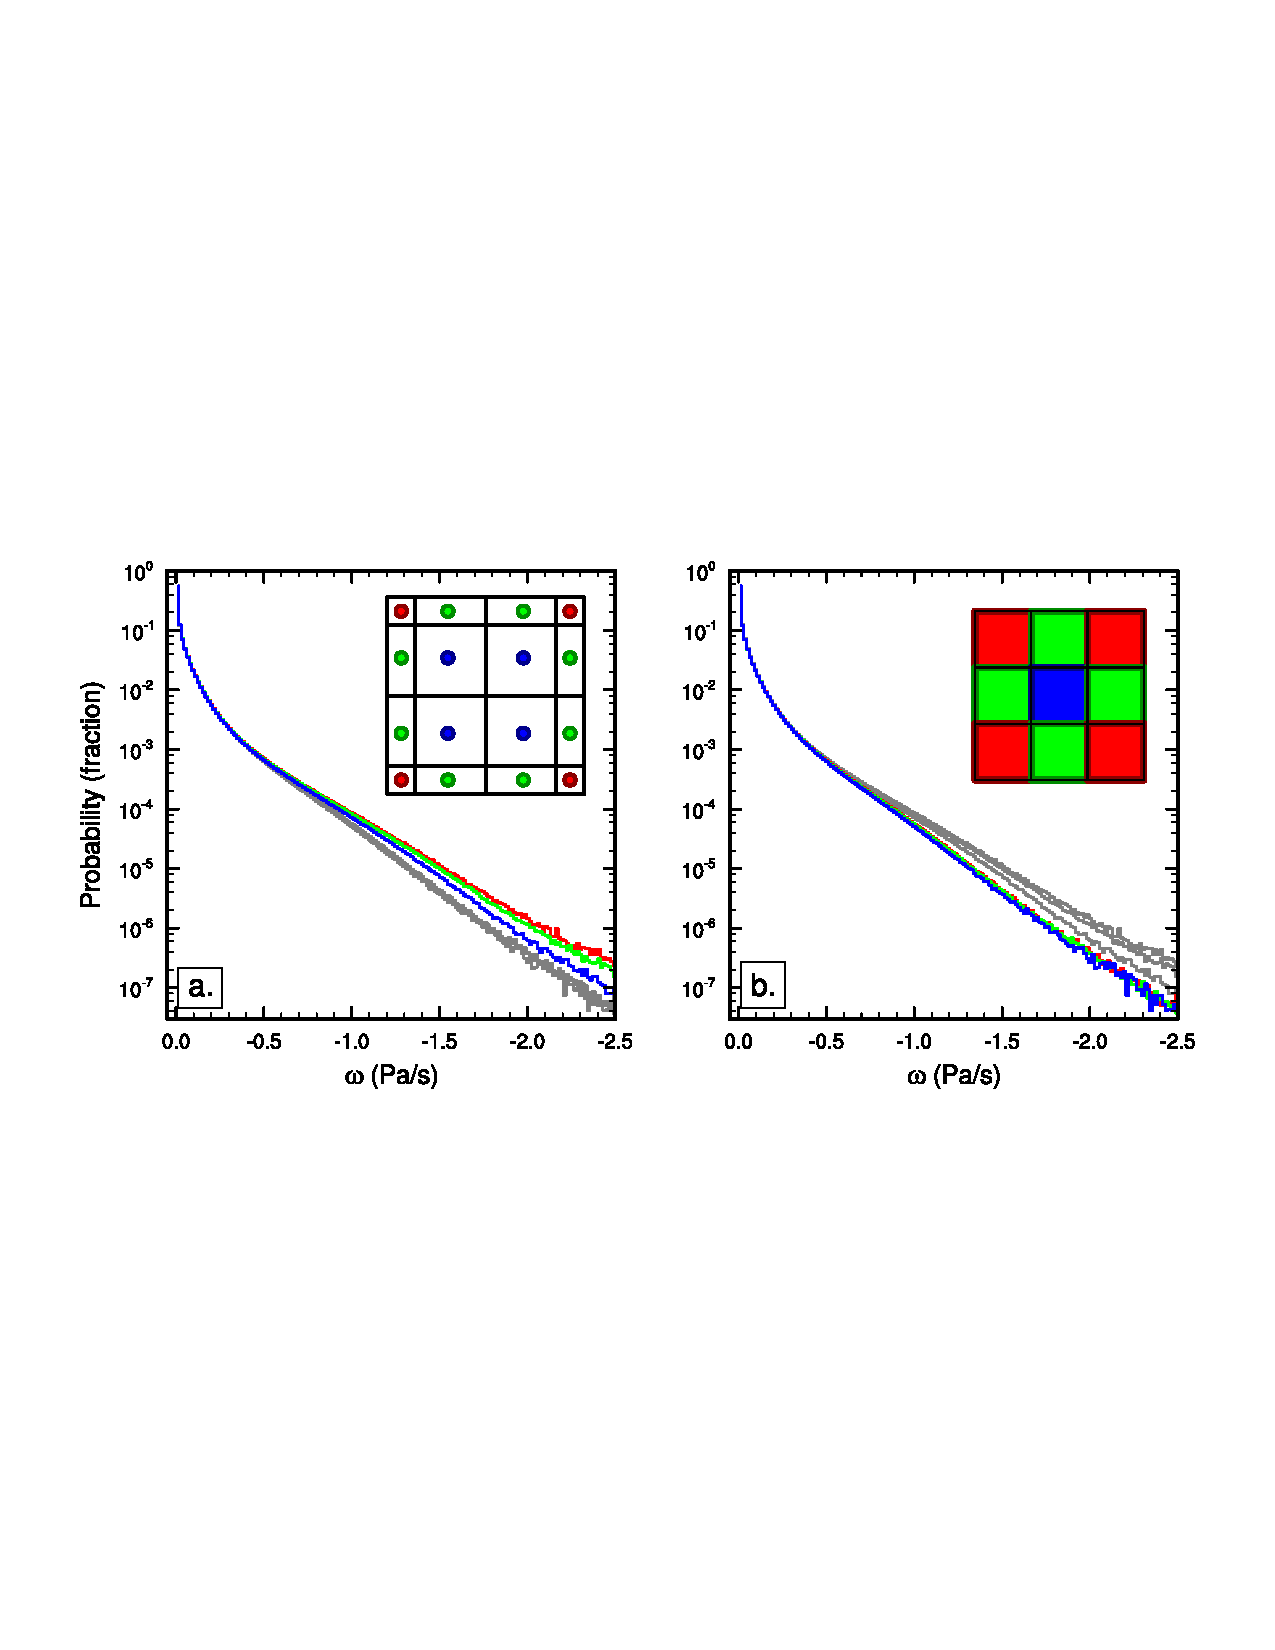
\includegraphics[width=35pc,angle=0]{chapter4/temp_pdf_200bins_30min_trX25min.pdf}\\
\end{center}
\caption{Probability density distribution of instantaneous upward $\omega$ in a pair of aqua-planet simulations using CAM4 physics. Figure is constructed from one year of six hourly data, at all vertical levels. (a) $ne30np4$ configuration conditionally sampled for interior, edge and corner node control volumes, and similarly (b) for the $ne30pg3$ configuration. The curves in (b) are overlain in (a) in grey, and similarly the curves in (a) are overlain in (b). Note the consistently larger magnitude $\omega$ for boundary nodes compared with interior nodes in (a), and that the bias is substantially reduced through mapping to a quasi-equal area physics grid.}\label{fig:omega-se-volumes}
\end{figure}

If the conventional physics-dynamics coupling paradigm is applied to CAM-SE, then the physics are to be evaluated at the GLL nodes, and a volume associated with the quadrature point should be defined. One approach to construct this grid is to decompose each spectral element into $(np-1) \times (np-1)$ subcells and then take the dual grid of this subcell grid.  For cubed-sphere meshes, this dual grid will have a control volume associated with each quadrature point. These control volumes will be triangles for the cube corner quadrature points and quadrilaterals for all remaining quadrature points.  Newton iteration can than be used to adjust the corners of these control volumes so that their spherical area exactly match the Gaussian weight multiplied by the metric term (these weights are used for integrating the basis functions over the elements and can therefore, in this context, be interpreted as areas).  For cubed-sphere meshes, the Newton iteration can be replaced by a direct method if some of the quadrilaterals are replaced by pentagons giving additional flexibility in matching the spherical area to the quadrature weights. Such a dual grid is shown in Figure \ref{fig:cv-grids}. This grid is used in the NCAR CESM (Community Earth System Model) coupler for passing states between ocean, atmosphere and land components since the current remapping method is finite-volume based and therefore requires control volumes (it is noted that methods exist that do not require control volumes for conservative interpolation, e.g., \cite{UT2015MWR}). Hence the components `see' an irregular atmospheric grid. Similarly, the parameterizations in the atmosphere `see' a state that is anisotropically sampled in space \citep[see Figure 1 and 5 in ][]{KetAl2008JGR}.

\begin{figure}[t]
\begin{center}
\noindent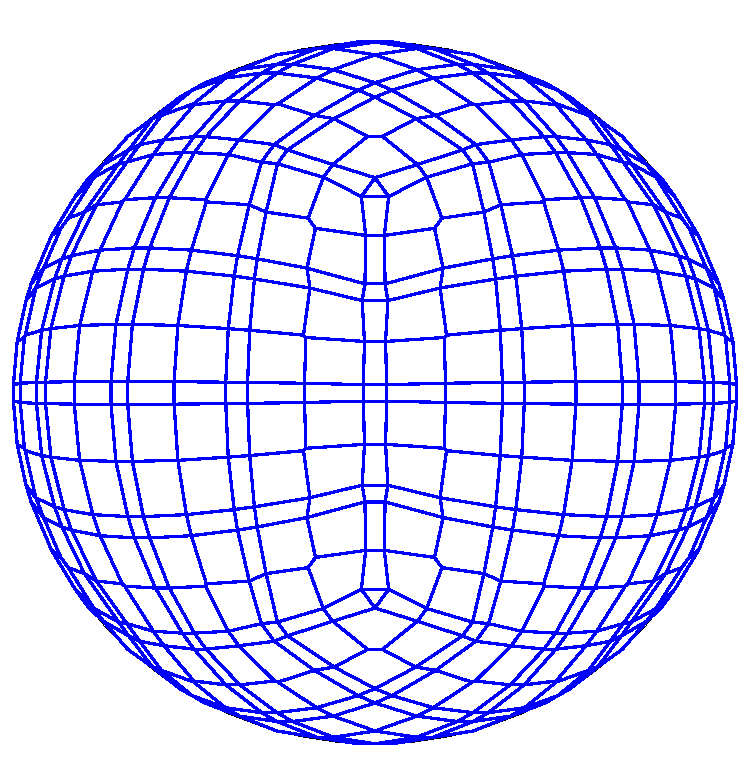
\includegraphics[width=15pc,angle=0]{chapter4/se_gll_cv_grid-eps-converted-to.pdf}\\
\end{center}
\caption{An example of control volumes constructed around GLL quadrature points ($ne4np4$) so that the spherical area of the control volumes exactly match the quadrature weight multiplied by the metric factor.}
\label{fig:cv-grids}
\end{figure}

The quadrature grid in element-based Galerkin methods is defined to perform mathematical operations on the basis functions, e.g., computing gradients and integrals, rather than evaluating the state variables for physics-dynamics coupling. One may argue that it would be more consistent to integrate the basis functions over quasi-equal area control volumes within each element and pass those control volume average values to physics rather than irregularly spaced quadrature point values. In this case when integrating basis functions over control volumes a grid-cell average value is more representative of the values near the extrema at the element boundary than the quadrature point value. The relationship between the nodal values, the basis functions and the proposed control volumes is illustrated schematically in one-dimension in parts (f) and (i) in Figure~\ref{fig:se-schematic}. 

\subsection{Methods}\label{sec:methods4}
Here we focus on CAM-SE, however, in principle the methods apply to any element-based high-order Galerkin model. The physics grid in CAM-SE is defined by sub-dividing each element using equi-angular gnomonic coordinate lines to define the sides of the physics grid control volumes (see the Appendix for details). Note that the element boundaries are defined by equi-angular gnomonic grid lines. The notation $pg=3$ refers to the configuration where the elements are divided into $pg\times pg=3\times 3$ equi-angular physics grid cells (see Figure \ref{fig:np4_pg3}) resulting in a quasi-equal spherical area grid resembling the cubed-sphere. Defining the physics grid by sub-dividing elements makes it possible to use the same element infrastructure as already used in CAM-SE, thereby facilitating its implementation. Here we make use of the $ne30np4$ and $ne30pg3$ grids that use GLL quadrature point physics grid (physics and dynamics grid coincide), and the same ($pg=3$) resolution quasi equal-area physics grids, respectively. In all configurations we use degree three Lagrange basis ($np=4$) and $ne\times ne=30\times 30$ elements on each cubed-sphere panel.

\begin{figure}[t]
\begin{center}
\noindent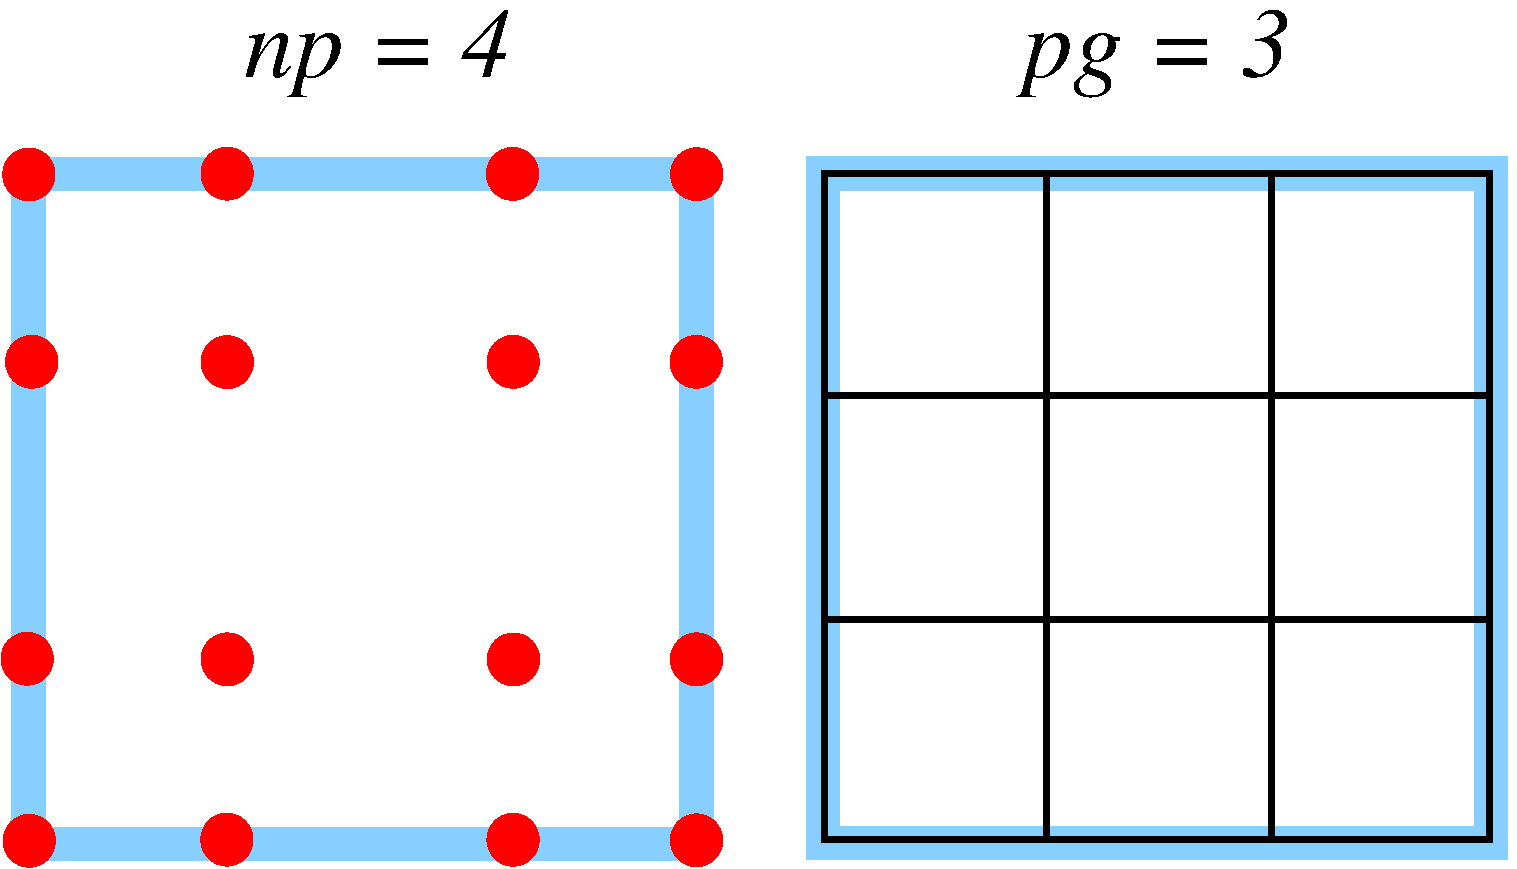
\includegraphics[width=25pc,angle=0]{chapter4/np4_pg3.pdf}\\
\end{center}
\caption{A schematic illustration of an element, indicating the relationship between (left) the dynamical core grid, and (right) the proposed quasi-equal area physics grid. The physics grid contains $pg\times pg=3\times 3$ grid cells in each element.}
\label{fig:np4_pg3}
\end{figure}

A consequence of separating physics and dynamics grids is that the atmospheric state must be mapped to the physics grid and the physics tendencies must be mapped back to the dynamics grid. This is discussed in separate sections below. When separating physics and dynamics grids it is advantageous to use a vertical coordinate that is static during physics-dynamics coupling. This was one motivation to switch to a dry-mass vertical coordinate in CAM-SE \citep{LetAl2018JAMES}; since dry mass remains constant throughout physics the dry-mass vertical coordinate remains fixed during physics-dynamics coupling. The dry mass coordinate subsequently evolves as floating Lagrangian layers by the dynamics \citep{L2004MWR} periodically mapped back to a reference hybrid-sigma-pressure coordinate after \cite{SB1981MWR}. All variables mapped between grids are collocated, layer-mean values \citep{LetAl2018JAMES}.
 
\subsubsection{Mapping state from dynamics grid (GLL) to physics grid (pg)}
The dynamics state is defined on the GLL grid in terms of temperature $T^{(gll)}$, zonal wind component $u^{(gll)}$, meridional wind component $v^{(gll)}$, and dry pressure level thickness $\Delta p^{(gll)}$. In the mapping of the atmospheric state to the physics grid it is important that the following properties are met:
\begin{enumerate}
\item conservation of scalar quantities such as mass and dry thermal energy,\label{prop1}
\item for tracers; shape-preservation (monotonicity), i.e., the mapping method must not introduce new extrema in the interpolated field, in particular, negatives,\label{prop2}
\item consistency, i.e., the mapping preserves a constant,\label{prop3}
\item linear correlation preservation, i.e., if field $A$ is a linear function of $B$, this relationship is still preserved \citep[see, e.g, equation 5 in][]{LT2011QJR}
\end{enumerate}
Other properties that may be important, but not pursued here, includes total energy conservation and axial angular momentum conservation. Total energy is a quadratic quantity that is inherently difficult to conserve unless one maps total energy requiring one to diagnose either temperature or momentum components. For example, enforcing total energy conservation locally using, e.g., \citet{L2004MWR}'s method where total energy and velocity components are remapped and temperature is a derived variable, has proven problematic (C. Chen, personal communication). Similarly conservation of axial angular momentum is problematic. Conservation of angular momentum requires one to interpolate the zonal and meridional components of momentum which creates large errors near the poles. To avoid the pole problem we interpolate contra-variant components of the momentum vector, which violates axial angular momentum conservation.

We argue that the most consistent method for mapping scalar state variables from the GLL grid to the physics grid is to integrate the Lagrange basis function representation (used by the SE dynamical core) over the physics grid control volumes, i.e., integrate the basis function representation of $\Delta p^{(gll)}\times T^{(gll)}$ and $\Delta p^{(gll)}$ over the physics grid control volume \citep[see, e.g., ][]{LTOUNGK2017MWR,UT2015MWR}
\begin{eqnarray}
\Delta p^{(pg)}&=&\frac{1}{A^{(pg)}}\int_{A^{(pg)}}\Delta p^{(gll)}\, dA,\\
T^{(pg)}&=&\frac{}{A^{(pg)}\Delta p^{(pg)}}\int_{A^{(pg)}}T^{(gll)}\Delta p^{(gll)}\, dA,
\end{eqnarray}
where $A^{(pg)}$ is the physics grid area. The integrals are numerically computed using the GLL quadrature rule on each physics grid element, which exactly (to machine precision) integrates the basis functions over the $pg$ control volumes \citep{LTOUNGK2017MWR}. Thermal energy and dry air mass is conserved and the mapping is consistent. For the wind, which is a vector, the zonal and meridional wind components are mapped by transforming to contra-variant wind components, evaluating the basis function representation thereof at the equi-angular center of the physics grid control volumes and then transformed back to latitude-longitude coordinate system winds. All of the operations are local to the element and do not require communication between elements.

The mapping of tracers is more problematic since the SE basis function representation is oscillatory although the shape-preserving filter guarantees shape-preservation at the GLL nodes \citep{GTS2014JCP}. To avoid this issue we use the CAM-SE-CSLAM version of CAM-SE \citep[Conservative Semi-Lagrangian Multi-tracer transport scheme][]{LTOUNGK2017MWR}, where tracers are advected on the $pg=3$ physics grid using the inherently mass and linear-correlation preserving CSLAM algorithm. Note that in CAM-SE-CSLAM the dry mass internally predicted by CSLAM, $\Delta p^{(cslam)}$, is, by design, equal to $\Delta p^{(gll)}$ integrated over the CSLAM/physics grid control volume \citep{LTOUNGK2017MWR}. Since the tracer grid and physics grids are co-located and $\Delta p^{(pg)}=\Delta p^{(cslam)}$ then the  mass conservation, correlation preservation, consistency and shape-preservation constraints are inherently fulfilled.
%
\subsubsection{Mapping tendencies from physics grid (pg) to dynamics grid (GLL)}
The physics tendencies are computed on the finite-volume physics grid and are denoted $f_T^{(pg)}$,$f_u^{(pg)}$,$f_v^{(pg)}$, and $f_m^{(pg)}$. Note that dry air mass is not modified by physics and hence there is no tendency for dry mass,  $f_{\Delta p}\equiv 0$. Also, it is important to map tendencies and not state from the physics grid to GLL grid otherwise one will get spurious tendencies from mapping errors when the actual physics tendency is zero (unless a reversible map is used).

It is important that this process:
\begin{enumerate}
\item for tracers; mass tendency is conserved,
\item for tracers; in each tracer grid cell the mass tendency from physics must not exceed tracer mass available in tracer grid cell (it is assumed that the physics tendency will not drive tracer mixing ratio negative on the physics grid),\label{item:phys2fvm_consistency}
\item linear correlation preservation,
\item consistency, i.e., the mapping preserves a constant tendency.
\end{enumerate}
Other properties that may be important, but not pursued here, includes total energy conservation (incl. components of total energy) and axial angular momentum conservation. Scalar variables are mapped from the physics grid to GLL grid using a tensor-product Lagrange interpolation in two dimensions (i.e., we assume that the pressure variations in the vertical are small). The local coordinates on a cubed-sphere are discontinuous at the element edges so the interpolation requires special attention at the cube corners and edges. The details are provided in the Appendix. Lagrange interpolation preserves a constant (including zero) and linear correlations. Tracer and physics grids are co-located so tracer mass, tracer shape, and tracer correlations are trivially preserved on the tracer grid; and the inconsistency in point \ref{item:phys2fvm_consistency} above will not appear. 

Mapping from $pg$ to GLL grids while conserving mass was found to be difficult without excessive grid imprinting at element edges. Mass-conservation (using conventional finite-volume methods) requires a control volume to be defined around the GLL points \cite[see Figure \ref{fig:cv-grids} in this paper or Figure 8b in ][]{UDJ2016MWR}. These volumes are artificial and not consistent with the SE method. Integrating the CSLAM reconstruction of water tracers of such artificial control volumes led to GLL node grid imprinting in the mapping and will not preserve a constant mixing ratio since the mapping of $\Delta p^{(pg)}$ to GLL will not yield the GLL node value for dry pressure-level thickness (i.e., the maps are not reversible).  A reversible map requires that the number of degrees of freedom on the source mesh ($pg3$ has 9 degrees of freedom) equal the number of degrees of freedom on the target mesh ($np4$ grid has 16 degrees of freedom). This condition is violated by construction for individual elements.

It was also found important to use an interpolator that is smooth across element boundaries. Using an algorithm that only uses information from an element of control volumes will (at best) be $C^0$ at the element boundaries and therefore lead to boundary node grid imprinting. A stencil that extends beyond one element is therefore necessary. After much experimentation, the best results in terms of grid-imprinting were obtained with tensor-cubic interpolation (see the Appendix for details) and by using the CAM-SE-CSLAM configuration (which requires the same boundary exchange/communication as used in CSLAM).

\subsubsection{Time splitting and physics-dynamics coupling}

The physics and dynamics are integrated in time using a sequential-update approach \citep[e.g.,][]{W2002MWR}. The dynamical core is sub-cycled over the (usually) longer physics time-step, $\Delta t_{phys}$, e.g., the vertical remapping time-step $\Delta t_{remap}$ is cycled $nsplit$ times, totaling to $\Delta t_{phys}$. In CAM-SE, a fraction of the physics forcing, e.g., $f_q \times \Delta t_{remap}$ is applied at the beginning of each $nsplit$ vertical remap subcycles, such that the full forcing ($f_q \times \Delta t_{phys}$) is realized over the course of a physics time-step. This approach of dribbling the tendencies over sub-intervals has the advantage of reducing gravity wave noise \citep{TJ2016GMD}, but may disrupt tracer mass conservation \citep{water-leak}. In CAM-SE-CSLAM, all but the tracer mass quantities are dribbled, with tracer mass receiving the full physics update, e.g., $f_q \times \Delta t_{phys}$, applied only at the beginning of the first remap sub-cycle, and thereby conserving tracer mass. This is the $ftype=2$ configuration described in detail in Section 3.6.3 in \cite{LetAl2018JAMES}.

In the SE integration of the equations of motion on the GLL grid the water species are needed in the computation of the pressure gradient force and generalized expressions for heat capacity at constant pressure $c_p$, etc. Hence the mixing ratios for water vapor and dynamically/thermodynamically active condensates (e.g., cloud liquid and cloud ice) are needed on the GLL grid. We have chosen to advect the water species on the GLL grid using the SE method as well as on the physics grid using CSLAM. Every time physics updates the water species on the CSLAM grid, a forcing term (equal to the difference between updated CSLAM water variables and the SE values) is applied to the GLL water variables using dribbling so that the CSLAM solution and SE solution for water species are tightly coupled. 

\subsection{Results}\label{sec:results4}

A hierarchy of idealized model configurations are presented in order to elucidate the differences between CAM-SE and CAM-SE-CSLAM (available from the CESM2.1 release; \url{https://doi.org/10.5065/D67H1H0V}). Here, the configurations are presented in order of increasing complexity, each with a pair of approximately $1^{\circ}$ simulations, pertaining to the $ne30np4$ (CAM-SE) and $ne30pg3$ (CAM-SE-CSLAM) grids, and a $\Delta t_{phys}$ = 1800 s.

\subsubsection{Moist Baroclinic Wave}

The moist baroclinic wave test case was developed as part of the `CESM Simple Models' project \citep{CESM_SIMPLER_MODELS}, and included in the release of CESM2. It is effectively the dry test-case of \cite{UMJS2014QJRMS}, but initialized with moisture and coupled to the Kessler moist physics routine \citep{K1969MM}. For more details on this test case \cite[which was part of the 2016 Dynamical Core Model Intercomparison Project, ][]{DCMIP16}, see Section 4.1 in \cite{LetAl2018JAMES}. A measure of the uncertainty in the reference solution, the $L_2$ difference norm between two high-resolution solutions using different dynamical cores, was also presented in \cite{LetAl2018JAMES} and provided again here in Figure \ref{fig:norm}. The $L_2$ norm between CAM-SE and CAM-SE-CSLAM lies below the uncertainty of the reference solution, indicating their differences are insignificant.

\begin{figure}[t]
\begin{center}
\noindent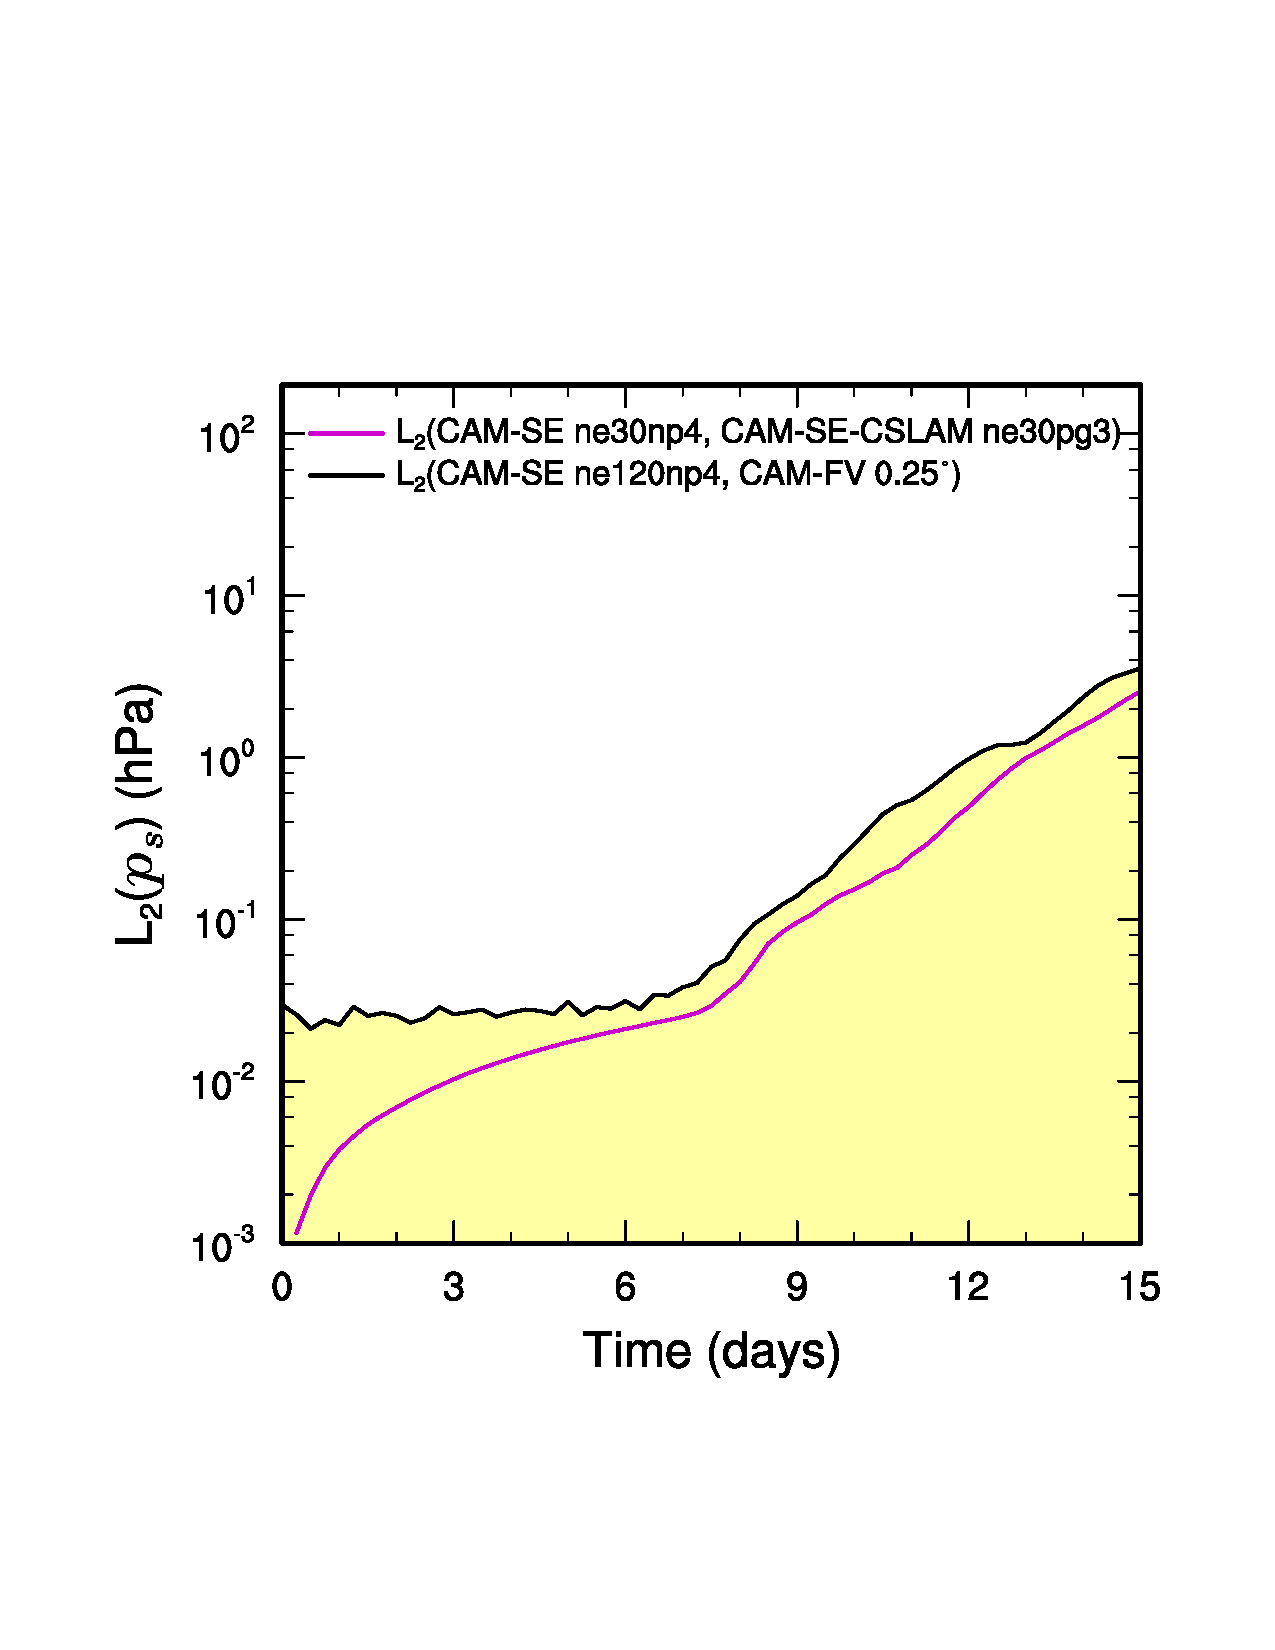
\includegraphics[width=20pc,angle=0]{chapter4/temp_l2.pdf}\\
\end{center}
\caption{$L_2$ difference norms of the surface pressure field, $p_s$, in the moist baroclinic wave simulations. $L_2$ values lying within the yellow region fall below the estimate of the uncertainty in the reference solution (black curve), computed as the difference norm between two approximately $0.25^\circ$ resolution versions of CAM, the spectral-element and finite-volume (CAM-FV) dynamical cores.}
\label{fig:norm}
\end{figure}

The flow field of the baroclinic wave test is used to drive the terminator ``toy"-chemistry test of \cite{LCLVT2015GMD,LTOUNGK2017MWR}. The terminator test is used to assess linear-correlation preservation using two reactive species advected across the terminator line. The model is initialized with species for which their weighted sum, $Cl_y$, is a constant (constant surface pressure and constant mixing ratio;$\ Cl_y = Cl + 2Cl_2 = 4\times 10^{-6}\ kg/kg$), such that if tracer correlations are preserved, then the column-integrated weighted sum of the species should not vary in time. Figure \ref{fig:term} provides a snapshot of the vertically integrated weighted sum of species at day 15. In CAM-SE, the tracer correlations are not preserved at day 15 and the field is populated by overshoots and undershoots. In contrast, by day 15, CAM-SE-CSLAM still conserves tracer correlations to within machine precision, consistent with the previous results of this test-case initialized with a dry baroclinic wave \citep{LTOUNGK2017MWR}. 

\begin{figure}[t]
\begin{center}
\noindent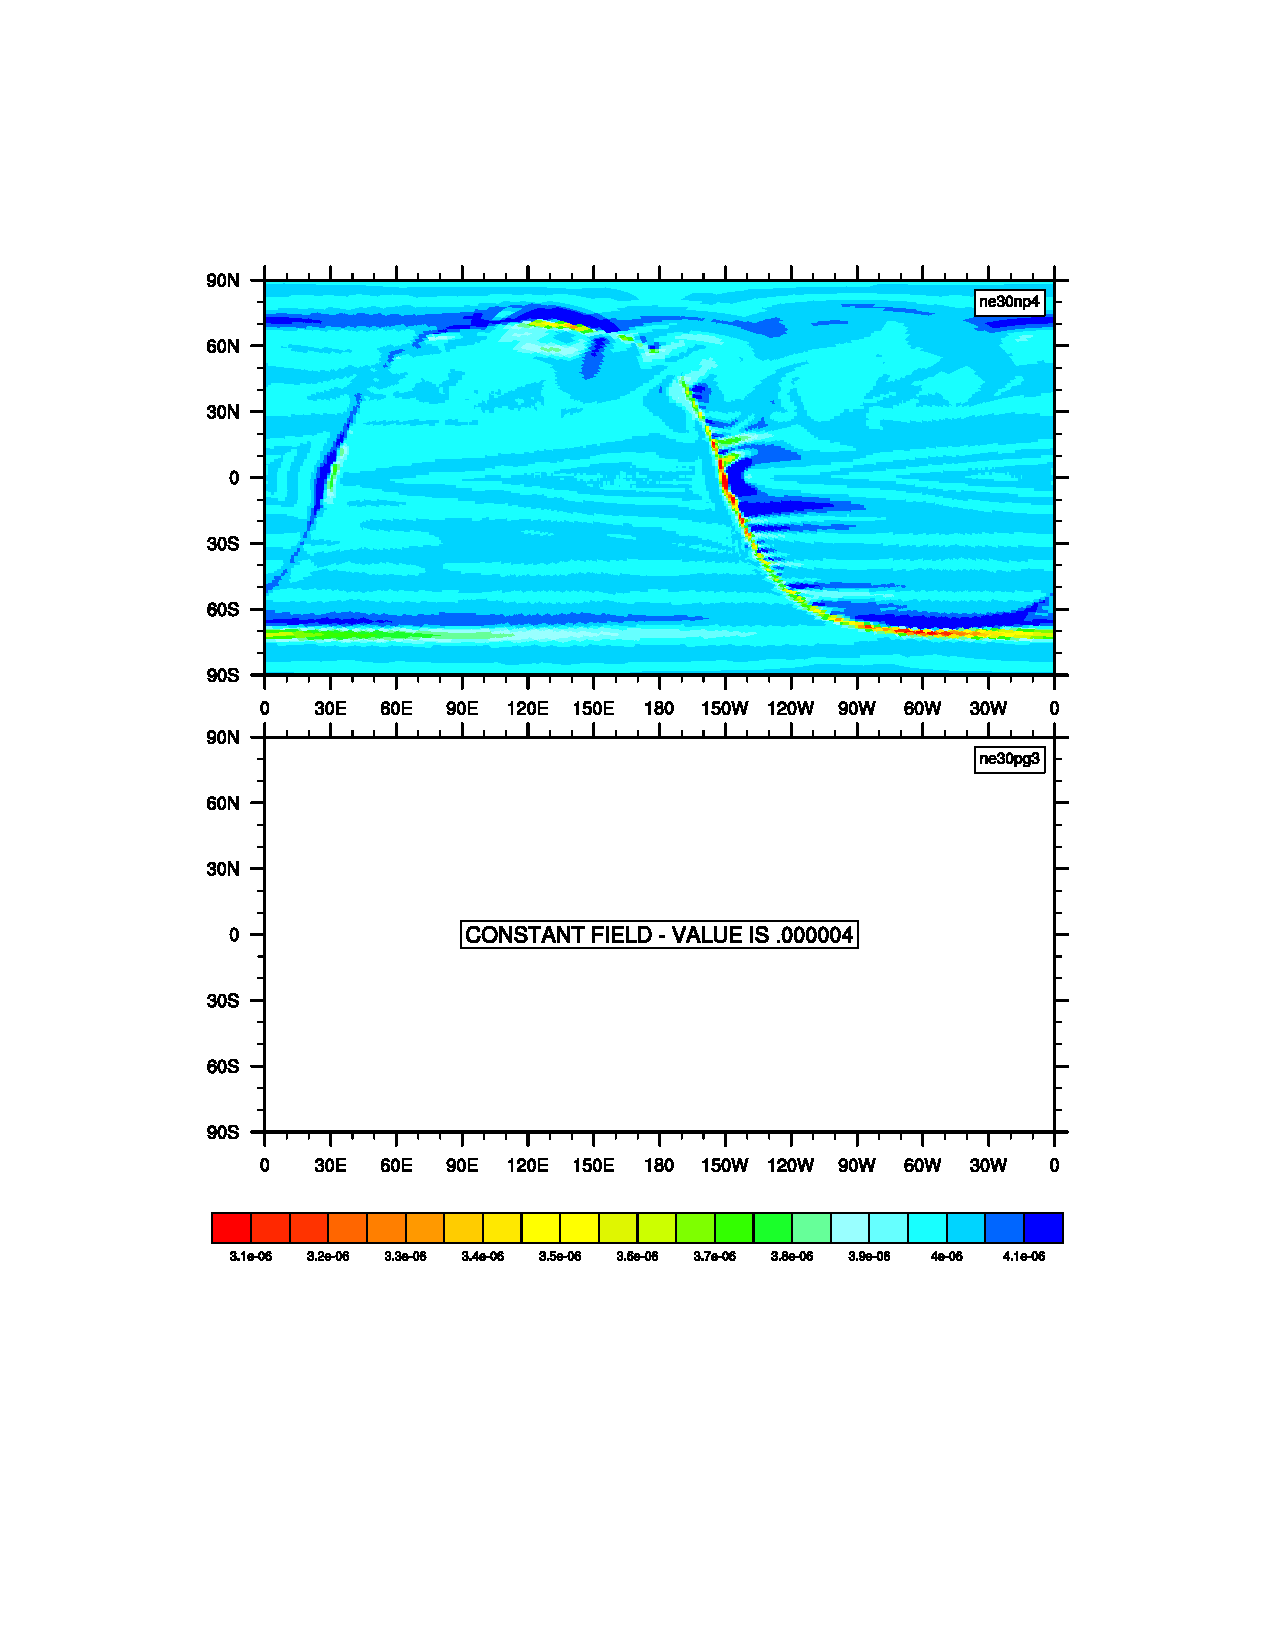
\includegraphics[width=25pc,angle=0]{chapter4/terminator_iCLy.pdf}\\
\end{center}
\caption{Results of the terminator ``toy"-chemistry test. Snapshot of the total column integrated, weighted sum of the species,$\ \left< Cl_y \right> = \left< Cl \right> + \left< 2Cl_2 \right>$, in kg/kg, at day 15 of the moist baroclinic wave test. (Top) CAM-SE, (Bottom) CAM-SE-CSLAM.}
\label{fig:term}
\end{figure}

\subsubsection{Aqua-planets}

Two year long aqua-planet simulations are performed using CAM-SE and CAM-SE-CSLAM, using the CAM4 physics package \citep{CAM4}, as discussed in Section \ref{sec:nodeproblem}. Away from the grid-scale, the mean states in the two models are very similar. Figure~\ref{fig:zonal} shows the zonal-mean climatological precipitation rates in CAM-SE and CAM-SE-CSLAM. Considering how sensitive this aqua-planet configuration is to design choices in CAM-SE \citep{LetAl2018JAMES}, it is somewhat unexpected that the zonal means look so similar to one another. 

\begin{figure}[t]
\begin{center}
\noindent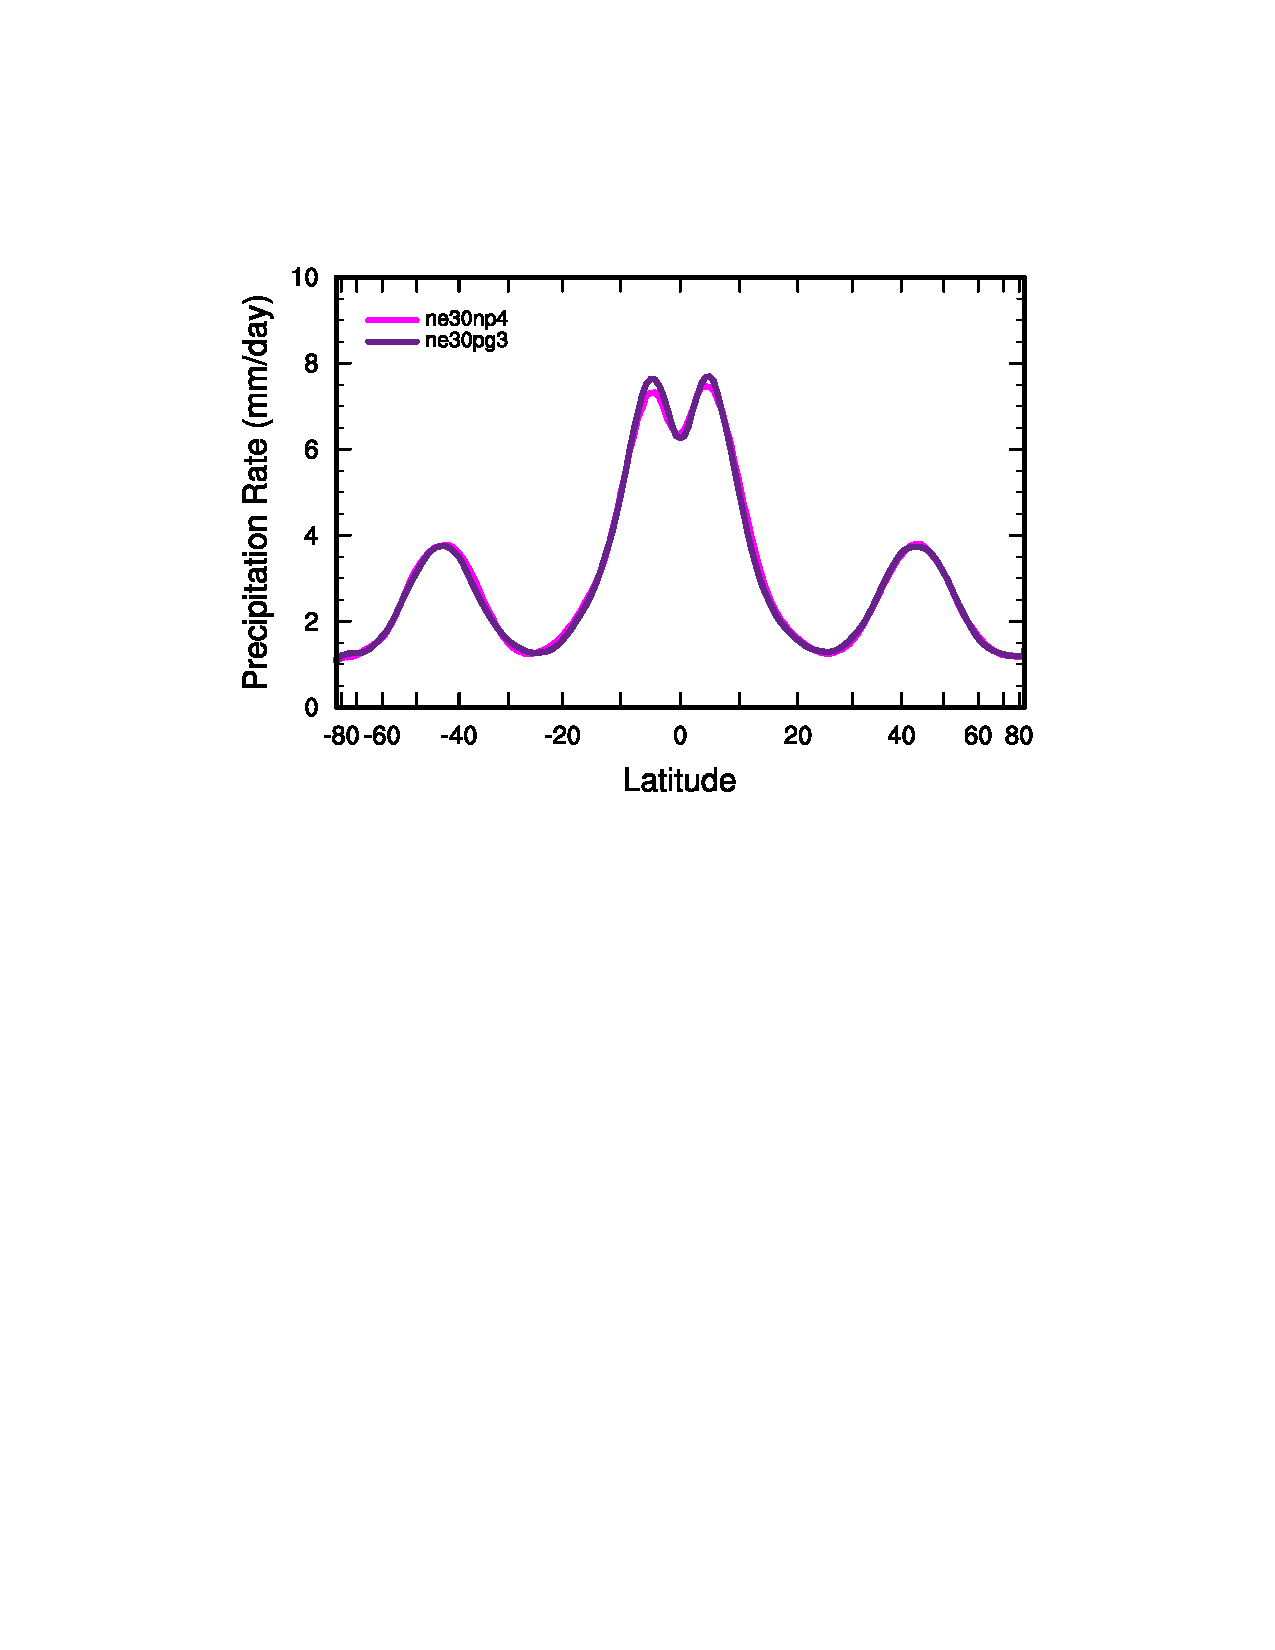
\includegraphics[width=20pc,angle=0]{chapter4/temp_dzonal.pdf}\\
\end{center}
\caption{Climatological zonal-mean total precipitation rate in the aqua-planets, computed from a pair of year long simulations.}
\label{fig:zonal}
\end{figure}

A plot similar to Figure \ref{fig:omega-se-volumes}a is constructed for the CAM-SE-CSLAM simulation, a probability density distribution of upward $\omega$ conditionally sampled based on location within the element. Like Figure \ref{fig:omega-se-volumes}a, Figure \ref{fig:omega-se-volumes}b divides up the control volumes by corner, edge and interior cells. Through the use of the quasi-equal area physics grid, the dynamical core state appears more or less independent of location within the element, a marked improvement over CAM-SE. Since the state is approximately independent of in-element location, it follows that the physics forcing, which is evaluated from the dynamical core state, may be expected to also show an improvement in grid-imprinting. 

The low-level, mean and variance of the temperature tendencies from the physics, on the GLL grid, $f_T^{(gll)}$, in the two simulations are shown in Figure \ref{fig:tendency_imprint}. The mean states in the two models resemble one another, consistent with the zonal mean precipitation rates (Figure~\ref{fig:zonal}). The mean physics tendencies contains modest grid imprinting in CAM-SE (barely visible near the storm-track regions), while in the variance field, grid imprinting is both ubiquitous and unmistakable. The variance is larger on boundary nodes, manifesting as a `stitching' pattern resembling the cube-sphere grid. In CAM-SE-CSLAM, the grid imprinting is all but eliminated based on the mean and variance of the physics tendencies (Figure~\ref{fig:tendency_imprint}), consistent with our expectation.

The global mean and variance of the low-level physics tendencies are marginally lower in CAM-SE-CSLAM compared with CAM-SE on the GLL grid (by about 1\% and 6\% for the mean and variance, respectively; Figure~\ref{fig:tendency_imprint}). While these differences may be small, and potentially insignificant, they are consistent with the state on the GLL grid in the two simulations. Through re-creating Figure \ref{fig:omega-se-volumes}a, but using the $\omega$ field on the GLL grid in the CAM-SE-CSLAM run, the frequency of large magnitude $\omega$ values (less than -1.0 Pa/s) associated with interior, corner and edge nodes is slightly lower (not shown). This suggests that the lower magnitude physics forcing in CAM-SE-CSLAM impacts the state on the GLL grid, albeit modestly. Therefore the lower frequency of large magnitude $\omega$ in CAM-SE-CSLAM (Figure \ref{fig:omega-se-volumes}) may not be solely due to the smoothing effect of integrating the basis functions over control volumes, but also the lower magnitude physics tendencies feeding back onto the dynamical state.

As stated in Section \ref{sec:methods4}, the mapping of the state to the physics grid and the reverse interpolation of physics tendencies to the GLL grid is not total energy conserving. CAM has a global energy fixer \citep{WOHTTV2015JAMES} which can be used to estimate the errors associated with the mapping algorithms. To do so, it is presumed that there are no compensating mapping errors in going to and from the physics and dynamics grids, and that CAM-SE-CSLAM and CAM-SE have the same energy dissipation rates. Under these assumptions the spurious globally integrated total energy errors due to the mapping algorithm is estimated to be approximately 0.0025 $W/m^2$ in the aqua-planet simulations. In comparison, the dynamical core total energy dissipation is on the order of 0.1 $W/m^2$ \citep{LetAl2018JAMES}. 

\begin{figure}[t]
\begin{center}
\noindent\includegraphics[width=30pc,angle=0]{chapter4/QPC4_bar_skk.pdf}\\
\end{center}
\caption{Mean (left) and variance (right) of the low level temperature tendencies from the physical parameterizations on the GLL grid, with the $ne30np4$ configuration, (top row) and $ne30pg3$ configuration (bottom row), in a pair of year-long aqua-planet simulations. Grid imprinting is observed along the element boundaries in $ne30np4$, but is absent from the $ne30pg3$ simulation.}
\label{fig:tendency_imprint}
\end{figure}

\subsubsection{Held-Suarez with Topography}

Grid imprinting associated with the flow around obstacles is more problematic than that encountered on the aqua-planets. In order to diagnose grid imprinting due to topographic flow, an idealized Held-Suarez configuration \citep{HS1994} is outfitted with real world topography after \cite{FRETAL2000WMR,BETAL2006MWR}, and run for two years. Figure~\ref{fig:FHS-contours} shows the mean $\omega$ at two different vertical levels in the middle troposphere. {The data are presented as a raster plot on their respective unstructured grids, in order to delineate whether a particular value is associated with an interior, edge or element boundary node. 

At higher latitudes (e.g., the southern Andes), the flow is smooth, conforming reasonably to the underlying topography. At lower latitudes, over the Andes (between the equator and $20^{\circ}S$) or the Himalayas (from $20^{\circ}N$ to $30^{\circ}N$), there is a clear preference for extrema to occur at the element boundaries (Figure~\ref{fig:FHS-contours}). The vertical structure of $\omega$ in regions of strong grid-imprinting indicates full-troposphere upward/downward motion (not shown). Grid imprinting is therefore more common in regions of weak stratification, such as occurs in the deep tropics, with forced up-slope flow facilitating the release of gravitational instability. Resolved updrafts/downdrafts often align with the element boundaries due to its systematically tighter pressure gradients. 

\begin{figure}[t]
\begin{center}
\noindent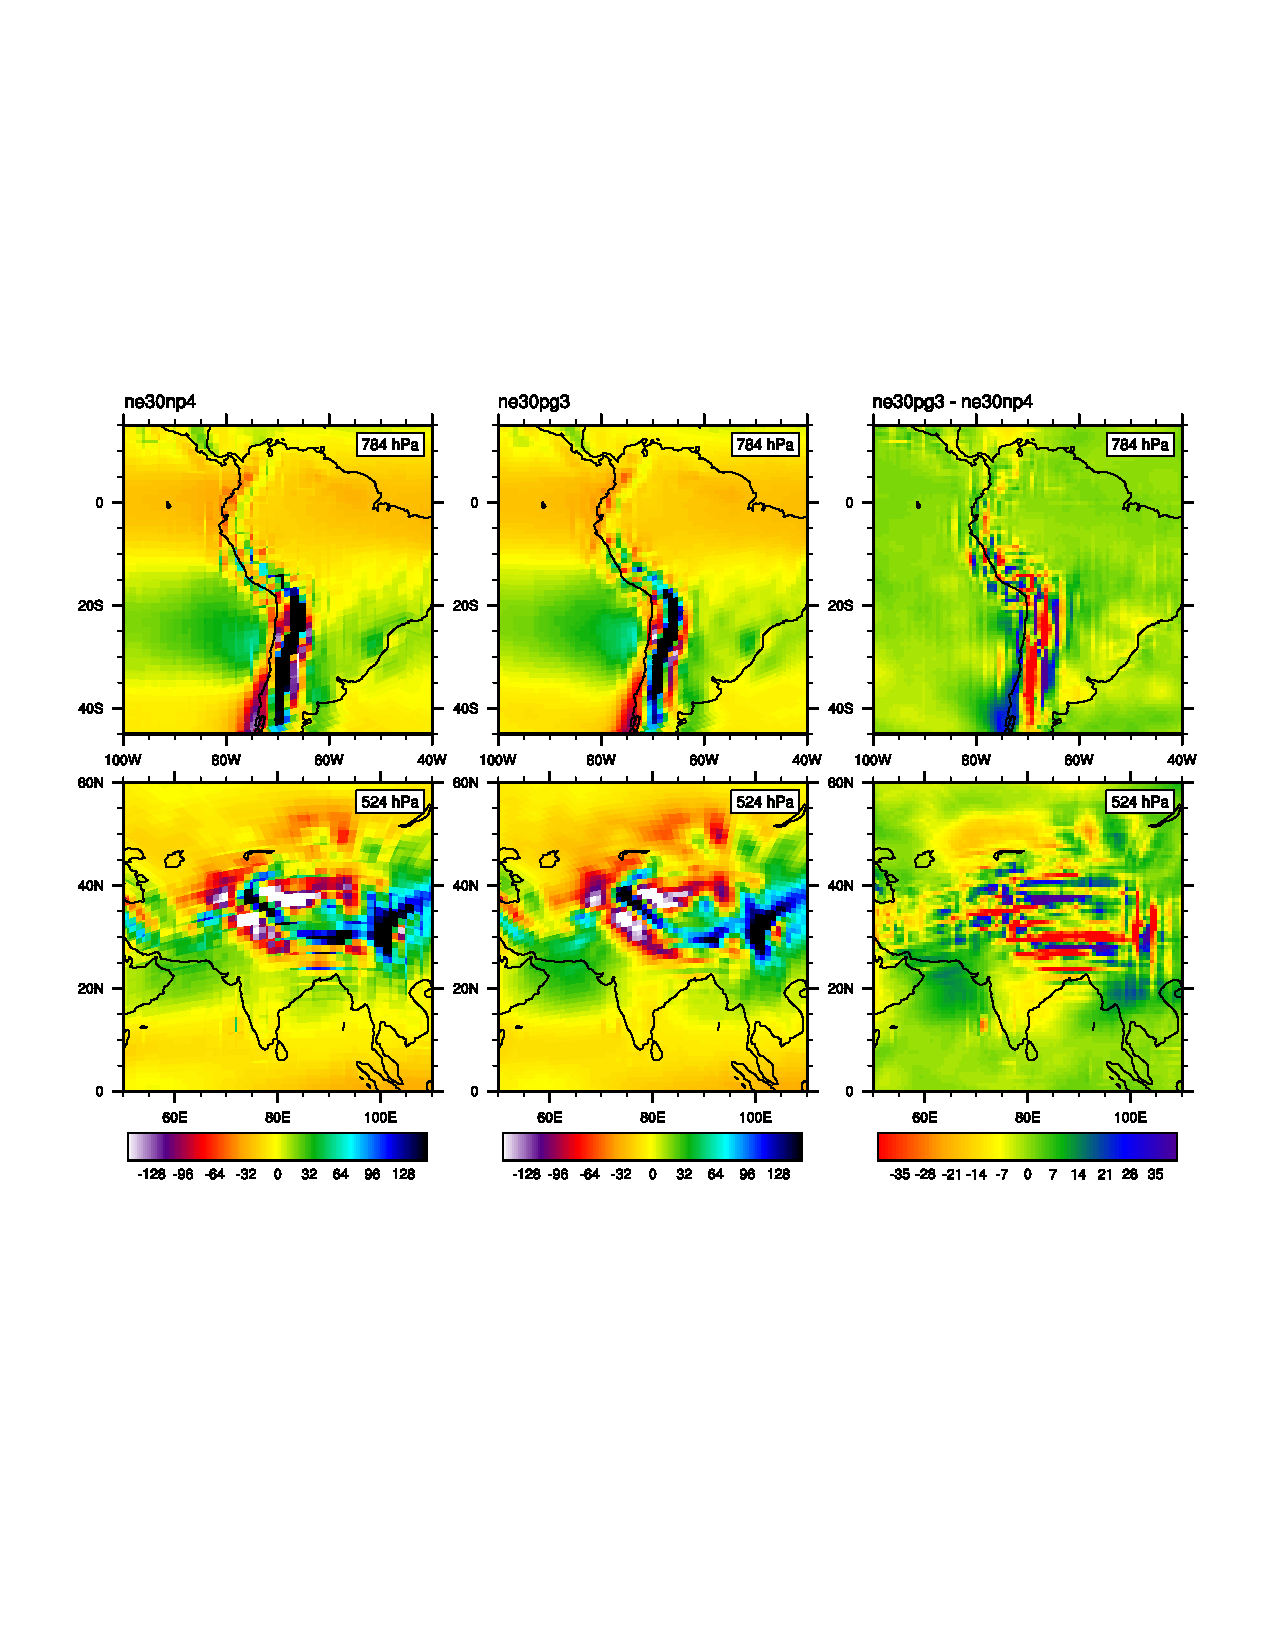
\includegraphics[width=30pc,angle=0]{chapter4/FHS-contours-CROP.pdf}\\
\end{center}
\caption{Mean $\omega$ at two model levels in the middle troposphere, in a Held-Suarez configuration outfitted with real world topography. (Left) CAM-SE state on the GLL grid, $ne30np4$, (Middle) CAM-SE-CSLAM state on the physics grid, $ne30pg3$ and (Right) their differences computed through bi-linear interpolation to a common latitude-longitude grid. The $\omega$ fields are computed from a 1200 day Held-Suarez simulation. The data are contoured according to a `cell fill' approach, in which the coupler grids (e.g, Figure~\ref{fig:cv-grids}) are used to delineate the vertices of the control volumes.}
\label{fig:FHS-contours}
\end{figure}

Through the use of the quasi-equal area physics grid, grid imprinting due to topographic flow is reduced (Figures~\ref{fig:FHS-contours}). The native topography lives on the physics grid, and the topography is mapped to the nodal points at run-time in CAM-SE-CSLAM. Mapping topography to the quadrature nodes ensures that no new extrema will be introduced to the boundary nodes, where the solution is least smooth. This effect can not be very large, since grid noise over topography is similar in CAM-SE and CAM-SE-CSLAM on the GLL grid (not shown). From the perspective of the physics grid, CAM-SE-CSLAM clearly mitigates the influence of grid-induced extrema on the state. This can be seen by comparing Figures~\ref{fig:FHS-contours}a and 10b, and their differences (Figure~\ref{fig:FHS-contours}c), which shows that the largest differences coincide with the element boundaries. The reduction in grid imprinting in this modified Held-Suarez configuration appears to be almost entirely a result of the smoothing effect of integrating the basis functions over the control volumes of the physics grid.

\subsubsection{AMIP type simulations}

A pair of 20 year-long AMIP type simulations are performed, using CAM, version 6 physics package (CAM6) and using perpetual year 2000 SST boundary conditions ($F2000climo$ compset in CESM2.0; \url{https://doi.org/10.5065/D67H1H0V}). Figure~\ref{fig:AMIP-region} shows the climatological precipitation fields in CAM-SE (left) and CAM-SE-CSLAM (middle), and over the same mountainous regions as in Figure~\ref{fig:FHS-contours}. The plots have some similar features to the $\omega$ field in the Held-Suarez runs; the greater variance at lower latitudes, and on the windward side of the mountains are broadly similar. CAM-SE-CSLAM has a lower spatial variance, e.g., the lack of extrema over the Andes at about $15^\circ$ S compared to CAM-SE, and the grid-scale precipitation peak over the Himalayas at about $30^\circ$ N. The difference plot (Figure~\ref{fig:AMIP-region}; right panel) is more broadly populated by blue, purple and white contours, indicating that CAM-SE has, in general, larger magnitude precipitation rates over high topography. The difference plots also highlight a couple of zonally aligned strips of anomalous precipitation, in particular, near the foot of the Himalayas in CAM-SE. These bands are in the same location as the bands of precipitation identified in CAM-SE in \cite{gmdd-8-4623-2015} (their Figure 7), but using CAM, version 5 physics, of which they argue are spurious in nature. 

\begin{figure}[t]
\begin{center}
\noindent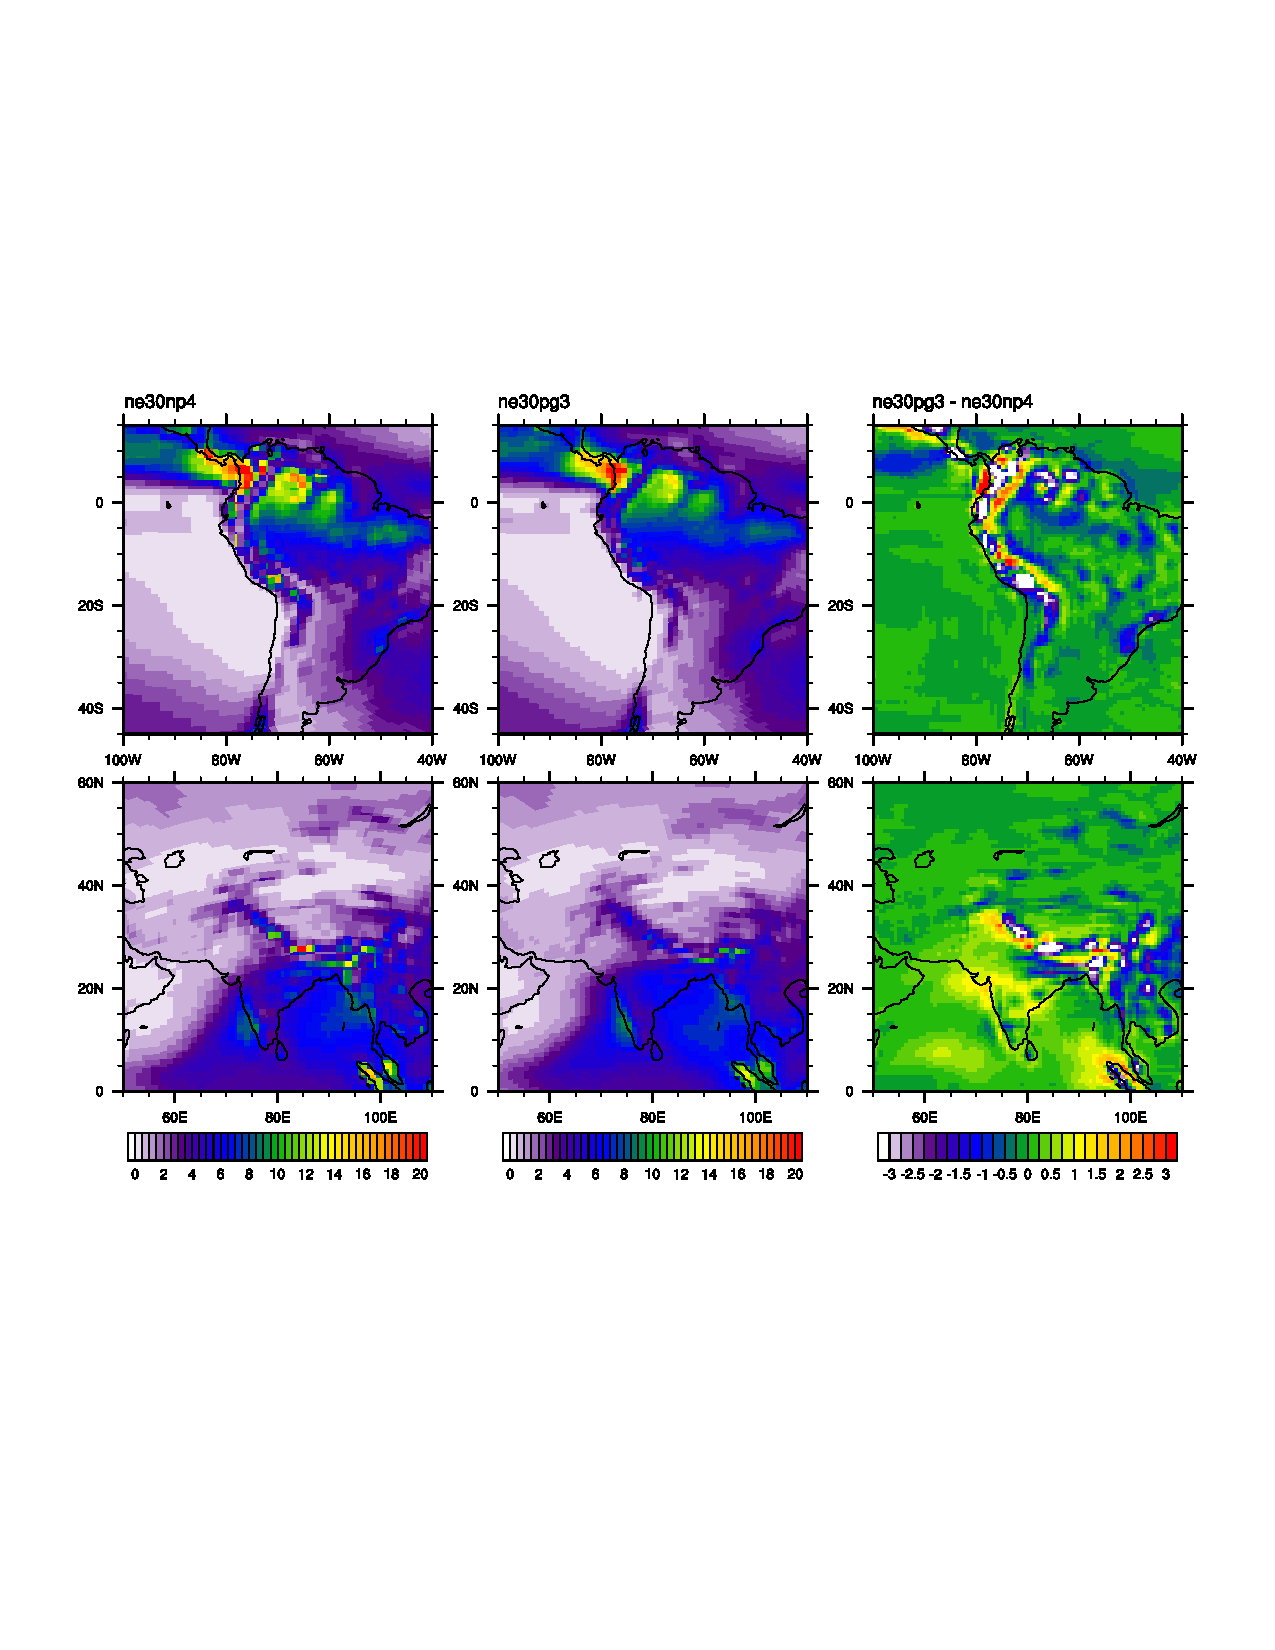
\includegraphics[width=30pc,angle=0]{chapter4/AMIP_regional.pdf}\\
\end{center}
\caption{Climatological total precipitation rate (in mm/day) computed from the final 19 years of a pair of 20 year long AMIP type simulations. (Left) CAM-SE, (middle) CAM-SE-CSLAM and (Right) their differences.}
\label{fig:AMIP-region}
\end{figure}

To assist in identifying whether a particular precipitation pattern is spurious, an $F2000climo$ simulation is carried out using the finite-volume dynamical core that uses a regular latitude-longitude $0.9^{\circ}\times 1.25^\circ$ grid \citep[CAM-FV; $f09$ grid; ][]{CAM5}. CAM-FV is the default low resolution model in CESM2.0, and with its smoothly varying grid, does not suffer from the Quadrature Node Problem (Section \ref{sec:nodeproblem}). Figure~\ref{fig:AMIP-global} shows the global precipitation fields in CAM-SE, CAM-SE-CSLAM and CAM-FV, compared to an observational dataset, the Global Precipitation Climatology Project (GPCP; 1979-2003) gridded dataset \citep{H2001JH}. The magnitude of the precipitation rates in all three models are higher than the GPCP dataset, primarily over land in the Tropics (note the lack of red contours in the GPCP dataset), which should be interpreted cautiously due to widely-accepted issues in constructing a reliable, gridded, global precipitation dataset. At lower latitudes, CAM-FV has lower spatial variance, and overall lower magnitudes, compared with CAM-SE. The GPCP dataset indicates that perhaps the precipitation rates in low-latitude mountainous regions in CAM-FV and CAM-SE are larger than in reality. Following suit, the reduction in magnitude and spatial variance in precipitation in these regions in CAM-SE-CSLAM may be interpreted as an improvement over CAM-SE.

\begin{figure}[t]
\begin{center}
\noindent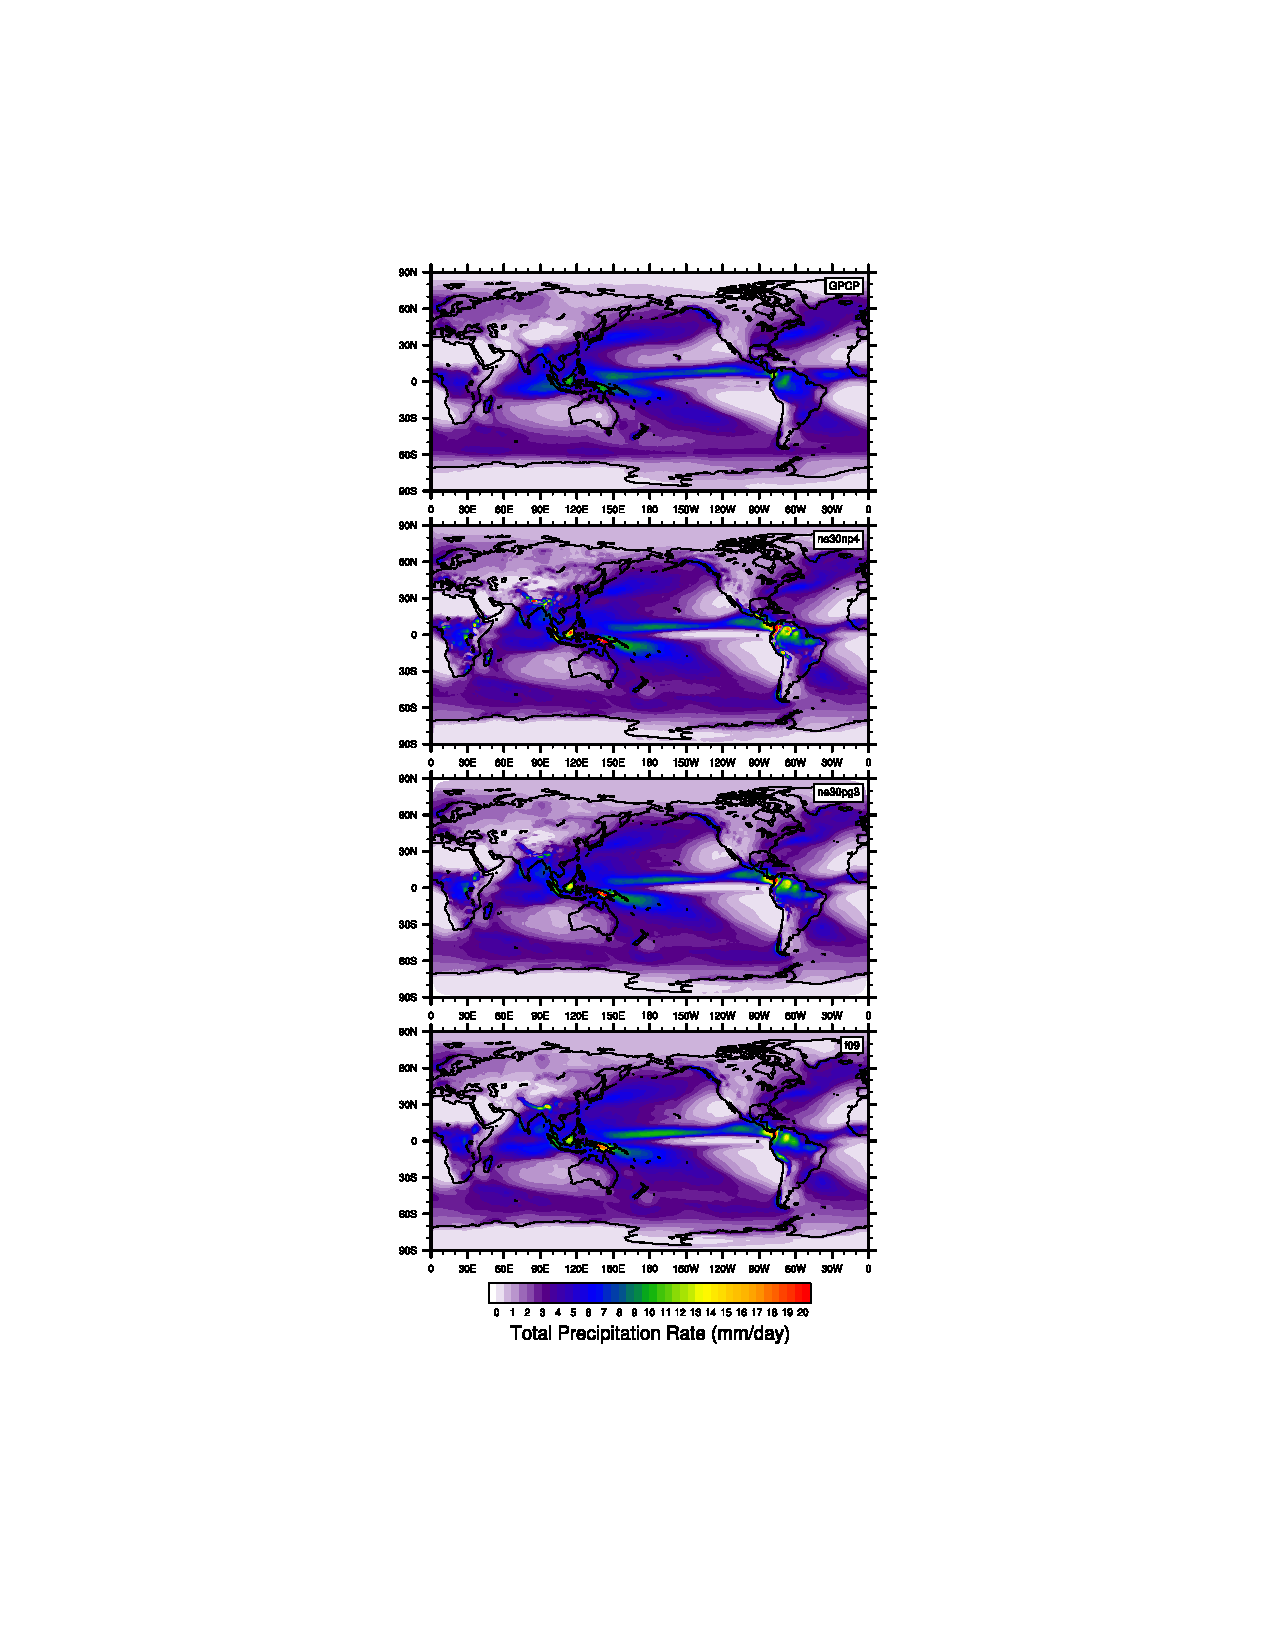
\includegraphics[width=14pc,angle=0]{chapter4/AMIP_global.pdf}\\
\end{center}
\caption{Climatological total precipitation rate computed from the final 19 years of a suite of 20 year long AMIP simulations, using CAM-SE (ne30np4), CAM-SE-CSLAM (ne30pg3) and CAM-FV (f09). The top plot is an observational product, the gridded GPCP climatological precipitation dataset.}
\label{fig:AMIP-global}
\end{figure}

\subsection{Conclusions}\label{sec:conclusions4}

Element-based high-order Galerkin Methods possess many of the attractive qualities recommended for next generation global atmospheric models. Among these, high-order accuracy is achieved with minimal communication between elements, allowing for near perfect scaling on massively parallel systems. Element communication amounts to a numerical flux applied to the element boundaries, reconciling overlapping solutions of adjacent elements but degrading the smoothness of the boundary nodes in the process (to $C^0$). For non-smooth problems, gradients are systematically tighter at the element boundaries, and local extrema often characterize the boundary nodes. This behavior is illustrated using NCAR's Community Atmosphere Model with Spectral Elements dynamics (CAM-SE) in an aqua-planet configuration, in a Held-Suarez configuration with real-world topography and in an AMIP type configuration.

The authors argue that the conventional physics-dynamics coupling paradigm, in which the physical parameterizations are evaluated on the dynamical core grid, exacerbates grid imprinting. A separate physics grid is proposed and implemented in CAM-SE, and referred to as CAM-SE-CSLAM, through dividing the elements into quasi-equal areas with equivalent degrees of freedom. The state is mapped to the physics grid with high-order accuracy through integrating CAM-SE's Lagrange basis functions over the control volumes. Control volumes near element boundaries now represent a state in the vicinity of the extrema produced through the boundary exchange, as opposed to the the nodal value itself. These control volumes are also compatible with a `large-scale state' as required by the physical parameterizations. The physical parameterizations are evaluated on the finite volume grid, and the forcing terms are mapped back to the dynamical core grid using a cubic tensor-product Lagrange interpolation. In aqua-planet simulations, evaluating the parameterizations on the physics grid removes any obvious dependence of proximity to the element boundary, resulting in a more realistic state with negligible grid imprinting. The mapping algorithm does not conserve total energy, but it is estimated that these errors are one to two orders of magnitude less than the total energy dissipation from the dynamical core.

In CAM-SE-CSLAM, the physics grid replaces the default CAM-SE quadrature point-based coupler grid (Figure~\ref{fig:cv-grids}) to compute fluxes between model components in the Community Earth System Model (CESM). The appeal here is two-fold. Through integrating the Lagrange basis functions over control volumes, one can be certain that the fluxes computed from this grid are a volume averaged flux. The same can not be said for CAM-SE, where artificial control volumes (with sizes proportional quadrature weights) are constructed around nodal values and assumed to represent the volume averaged state. The second advantage of the new coupler grid is that extrema occurring on boundary nodes may no longer influence other model components in simulations without rough topography. While grid imprinting is effectively eliminated in the aqua-planets, experiments with real-world topography (Held-Suarez and AMIP type configurations) reduces, but does not entirely eliminate, imprinting from the mean state. The quasi-equal area physics grid is nonetheless effective at mitigating numerical nuances associated with high-order element-based Galerkin methods, for non-smooth problems. 

Future work will focus on the impact of using a coarser, $pg\times pg=2\times 2$ physics grid configuration. The coarser physics grid may be more effective at reducing spurious noise over regions of rough topography, while potentially reducing the computational overhead. Any advantages of using a coarser resolution physics grid will be weighed against any potential reduction in a model's effective resolution.
 \label{sec:chapter4}

\newpage
\begin{center}
\section{Exploring a lower resolution physics grid in CAM-SE-CSLAM}
%\chapter{\bf{\normalsize Exploring a lower resolution physics grid in CAM-SE-CSLAM}}
\end{center}
%\addcontentsline{toc}{section}{\protect\numberline{}Exploring a lower resolution physics grid in CAM-SE-CSLAM}
%\addcontentsline{toc}{chapter}{\protect\numberline{}Exploring a lower resolution physics grid in CAM-SE-CSLAM}
\subsection{Introduction}\label{sec:intro}

Global atmospheric models fundamentally consist of two components. The dynamical core ({\em{dynamics}}), which numerically integrate the adiabatic equations of motion and tracer advection, and the physical parameterizations ({\em{physics}}), which compute the effects of diabatic and subgrid-scale processes (e.g., radiative transfer and moist convection) on the grid-scale. More out of convenience than anything else, the physics are evaluated on the dynamics grid, i.e., the physics and dynamics grids coincide. From linear stability and accuracy analysis of numerical methods, it is a common result that the shortest simulated wavelengths are not accurately represented by the dynamical core. Additionally, simulated downscale cascades result in an unrealistic collection of energy and/or enstrophy near the truncation scale, which may be observed from kinetic energy spectra in model simulations \citep{S2011LNCSE}. Some form of dissipation must be incorporated into models to mitigate these numerical artifacts near the grid scale \citep{JW2010LNCSE}. The unrealistic nature of the grid-scale led \cite{LH1997MWR} to speculate whether the physics should be evaluated on a grid that is more reflective of the scales actually resolved by the dynamical core.

Exploring the impact of different physics grid resolutions has so far been limited to models employing the spectral transform method \citep{LH1997MWR,W1999T,W2014PTRSL}. \cite{LH1997MWR} argued that passing under-resolved states to the physics may be especially problematic in spectral transform models, since the physics are evaluated on a latitude-longitude transform grid, and contains more degrees of freedom than the spectral representation to prevent aliasing of quadratic quantities. However, \cite{LH1997MWR} found that the spectral truncation of the physics tendencies damps errors that may result from passing an under-resolved state to the physics, although the extent to which these errors may still be present in the model is difficult to address. 

Another class of spectral transform models evaluate the quadratic terms using semi-Lagrangian methods, which are implicitly diffusive, relaxing constraints on the resolution of the transform grid. \cite{W2014PTRSL} experimented with different transform grid resolutions and concluded that the standard high resolution quadratic grid actually improves forecast skill over the use of a lower-resolution transform grid. They suggest that increasing the resolution of the transform grid simulates a kind of sub-grid variability on the spectral state, which is thought to be under-represented in global atmospheric models \citep{S2005QJR}. This is in principle the purpose of ``super-parameterization," in which a cloud resolving model is embedded in each grid cell to approximate sub-grid variability, and improves both diurnal and sub-seasonal variability in the model \citep{RKAG2003BAMS}.

After the physics tendencies are transformed into spectral space, it is possible to truncate the tendencies at any particular wave number in global spectral transform models. \cite{W1999T} conducted a pair of convergence tests using a spectral transform model; a conventional convergence test and one in which the spectral truncation of the physics tendencies is held fixed and the resolution of the dynamical core increased. In contrast to the realistic weather forecasts of \cite{W2014PTRSL}, \cite{W1999T} ran their model to equilibrium in an idealized climate configuration. When the physics and dynamics resolutions increase together, as in more typical convergence studies, the strength of the Hadley Cell increases monotonically with resolution. This sensitivity of Hadley Cell strength to horizontal resolution is a common result of global models at hydrostatic resolutions \citep[see][and references therein]{HR2017JCLIM}. But with the truncation wave number of physics tendencies held fixed, the Hadley Cell showed very little sensitivity to dynamical core resolution, resembling the solution for which the dynamics truncation wave number is equal to that of the lower resolution physics. \cite{HR2017JCLIM} speculated that these results suggest the scales of motion resolved by the dynamical core may be aliased to the lower resolution physics.

Global spectral transform models, while remarkably efficient at small processor counts, do not scale well on massively parallel systems. High-order Galerkin methods are becoming increasingly popular in climate and weather applications due to their high-parallel efficiency, high-processor efficiency, high-order accuracy (for smooth problems), and geometric flexibility facilitating mesh-refinement applications \citep[e.g.,][and the Energy Exascale Earth System Model; \url{https://e3sm.org/}]{Giraldo20083849,NCT2009CF,BSBDK2013TCFD}. High resolution climate simulations with NCAR's Community Atmosphere Model \citep[CAM;][]{CAM5} are typically performed using a continuous Galerkin dynamical core referred to as CAM-SE \citep[CAM Spectral Elements;][]{TES2008JPCS,DetAl2012IJHPCA,LetAl2018JAMES}. CAM-SE may be optionally coupled to a conservative, semi-Lagrangian tracer advection scheme for accelerated multi-tracer transport \citep[CAM-SE-CSLAM;][]{LTOUNGK2017MWR}. Tracer advection then evolves on an entirely separate, finite-volume grid which contains the same degrees of freedom as CAM-SE's quadrature node grid.

Element-based Galerkin methods are susceptible to grid-imprinting, and may need be considered when contemplating a particular physics grid \citep[][hereafter referred to as H18]{HL2018MWR}. Grid imprinting manifests at the element boundaries, since the global basis is least smooth ($C^{0}$; all derivatives are discontinuous) for quadrature nodes lying on the element boundaries, and the gradients (e.g., pressure gradients) are systematically tighter producing local extremes. Through computing the physics tendencies at the nodal points, element boundary extrema is also observed in the physics tendencies. 

H18 has shown that through evaluating the physics on the finite-volume tracer advection grid in CAM-SE-CSLAM, element boundary errors are substantially reduced, although still problematic in regions of steep terrain, at low latitudes. Through integrating CAM-SE's basis functions over the control volumes of the finite-volume grid, element boundary extrema is additionally weighted by the $C^{\infty}$ solutions (i.e., the basis representation is infinitely smooth and all derivatives are continuous) that characterize the interior of the element, and the state is smoother. Additionally, in defining an area averaged state, the finite-volume physics grid is made consistent with assumptions inherent to the physics, and is more appropriate for coupling to other model components (e.g., the land model), which is typically performed using finite-volume based mapping algorithms.

The CAM-SE-CSLAM finite-volume grid is defined through dividing the elements of CAM-SE's gnomonic cubed-sphere grid with equally spaced, equi-angular coordinate lines parallel to the equi-angular element boundaries, such that there are $3\times 3$ control volumes per element (hereafter referred to as $pg3$; see Figure~\ref{fig:overview}). While the physics grid in H18 is $pg3$, i.e., the physics and dynamics grids have the same degrees of freedom, the control volumes in $pg3$ encompass a region of the element in which their proximity to the element boundaries are not equal. Therefore, not every control volume in an element has the same smoothness properties. This may be avoided through defining a physics grid in which the elements are instead divided into $2\times 2$ control volumes (hereafter referred to as $pg2$; see Figure~\ref{fig:overview}). The control volumes of the $pg2$ grid all have the same proximity to the element boundaries, and should mitigate the element boundary noise that remains in the $pg3$ grid, and shown in H18.

In this study, we test the hypothesis that the coarser, $pg2$ physics grid is effective at reducing spurious noise at element boundaries, particularly over regions of rough topography. In addition, the recent trend towards running models at ever higher resolutions is an almost prohibitive computational burden. As the physics are responsible for over half of the computational cost in CAM-SE \citep{LetAl2018JAMES}, the improvement in computational performance using a coarser resolution physics grid is potentially significant. However, any advantages of using a coarser physics grid need be weighed against any potential reduction in simulation quality, e.g., possible aliasing of the resolved scales of motion by the coarser grid, as suggested by the results of \cite{W1999T}. Section \ref{sec:methods} describes the implementation of the $pg2$ grid into CAM-SE-CSLAM, and the idealized model configurations used throughout this study. Section \ref{sec:results} provides results of model simulations, to test the implementation of the mapping algorithms and identify any changes in grid imprinting, and in the resolved scales of motion, compared with the $pg3$ configuration. Section \ref{sec:conclusions} provides a discussion of the results and conclusions.

\subsection{Methods}\label{sec:methods}

Separating dynamics, tracer and physics grids introduces the added complexity of having to map the state from dynamics and tracer grids to the physics grid; and mapping physics tracer increments back to the tracer grid and physics increments needed by the dynamical core to the dynamics grid (see Figure \ref{fig:overview}). The dynamics grid in the case of CAM-SE-CSLAM refers to the Gauss-Lobatto-Legendre (GLL) quadrature nodes used by the spectral-element method to solve the momentum equations for the momentum vector $(u,v)$, thermodynamics equation for temperature ($T$), continuity equation for dry air mass ($\frac{1}{g}p$), and continuity equations for water vapor and thermodynamically and inertially active condensates \citep[see, e.g., ][ for details]{LetAl2018JAMES}. By tracer grid we refer to the $pg3$ grid on which CSLAM performs tracer transport of water vapor, condensates and other tracers. Although water vapor and condensates are being advected by the CSLAM scheme on the $pg3$ grid, these quantities are also needed on the GLL grid for the momentum equations and thermodynamic equation. Transport of water variables is also performed by the spectral-element method on the GLL grid. To avoid decoupling of water species on the CSLAM and GLL grids, the GLL water species are overwritten by the CSLAM values every physics time-step. This is explained in detail in H18.

\begin{figure}[t]
\begin{center}
\noindent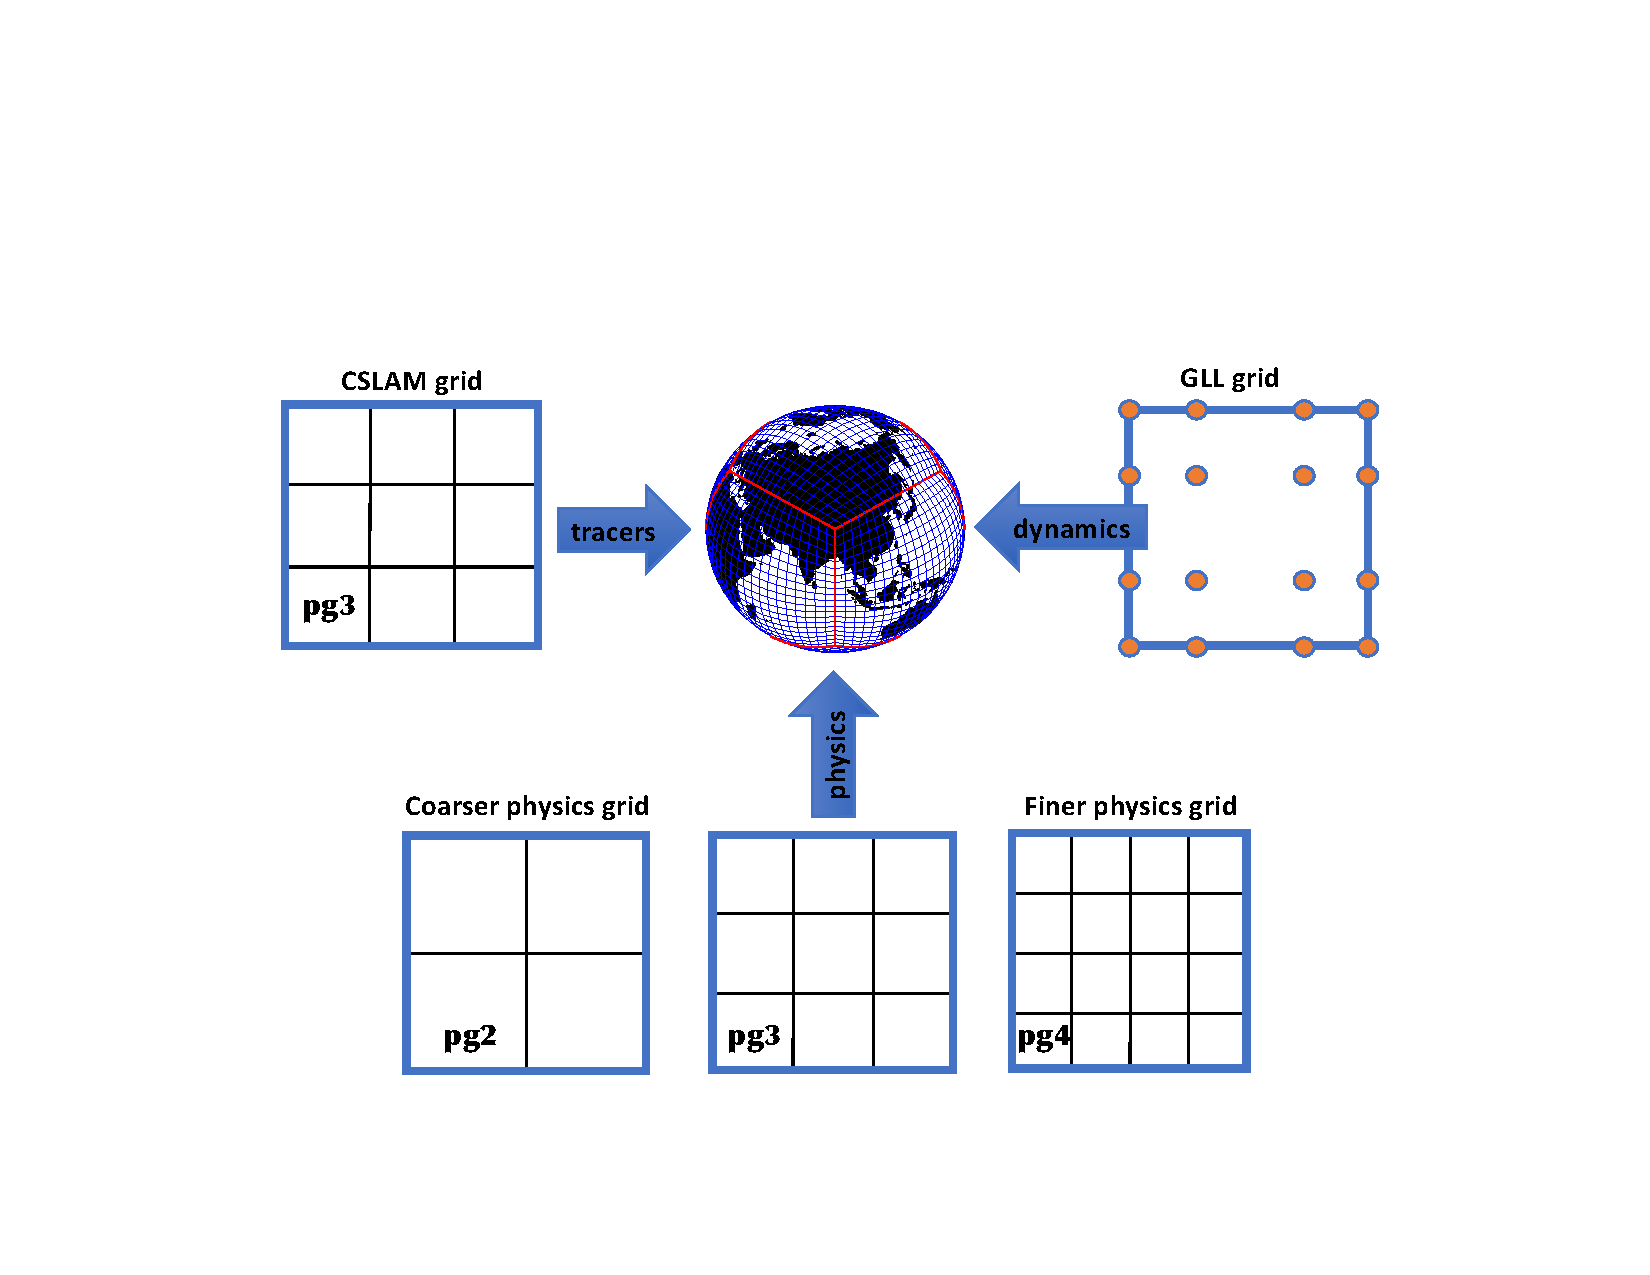
\includegraphics[width=35pc,angle=0]{chapter5/fig-overview.pdf}\\
\end{center}
\caption{An overview of the different grids in CAM-SE-CSLAM.}
\label{fig:overview}
\end{figure}

Similarly to the CAM-SE-CSLAM $pg3$ configuration, the dynamics state (momentum vector, temperature, dry pressure) must be mapped from the $GLL$ grid to the physics grid. Exactly the same algorithms as used in the $pg3$ configuration apply, i.e. momentum components are interpolated by evaluating the internal Lagrange basis functions (used in the spectral-element method) at the equi-angular (gnomonic) center of the $pg2$ cells and the Lagrange basis function representations of temperature and pressure are integrated over the $pg2$ control volumes. See H18 for details.

As compared to the $pg3$ configuration, the extra complication with the $pg2$ setup is that the tracer grid does not coincide with the physics grid, i.e. the tracer state needs to be mapped from the CSLAM grid ($pg3$) to the physics grid ($pg2$), and tracer increments computed by physics must be mapped from the physics grid back to the CSLAM grid. In order to describe the mapping algorithms between the grids some notation needs to be introduced.

The mapping algorithms are applied to each element $\Omega$ (with spherical area $\Delta \Omega$) so without loss of generality consider one element. Let $\Delta A^{(pg2)}_k$ and $\Delta A^{(pg3)}_\ell$ be the spherical area of the physics grid cell $A^{(pg2)}_k$ and CSLAM control volume $A^{(pg3)}_\ell$, respectively. The physics grid cells and CSLAM cells, respectively, span the element, $\Omega$, without gaps or overlaps
\begin{eqnarray}
\cup_{k=1}^{nphys^2}A^{(pg2)}_k=\Omega \text{ and } A^{(pg2)}_k \cap A^{(pg2)}_\ell = \emptyset \quad \forall k\ne \ell,\\
\cup_{k=1}^{nc^2}A^{(pg3)}_k=\Omega \text{ and } A^{(pg3)}_k \cap A^{(pg3)}_\ell = \emptyset \quad \forall k\ne \ell,
\end{eqnarray}
where $nc=3$ is the CSLAM grid resolution parameter and $nphys=2$ is the physics grid resolution parameter (following the Fortran code base), although the methods described here are valid for any arbitrary integer $nphys$ (e.g., $nphys=4$ is shown in Figure~\ref{fig:overview}). The overlap areas between the $k$-th physics grid cell and $\ell$th CSLAM cell are denoted
\begin{equation}
A_{k\ell}=A^{(pg2)}_k \cap A^{(pg3)}_\ell,
\end{equation}
(see Figure \ref{fig:area-schematic}) so that
\begin{equation}
A^{(pg2)}_k=\cup_{l=1}^{nc^2}A_{k\ell}.
\end{equation}
This overlap grid is also referred to as the {\em{exchange grid}}.

\subsubsection{Mapping tracers from $A^{(pg3)}$ to $A^{(pg2)}$ (CSLAM to physics grid)}\label{sec:nctopg}
The CSLAM and physics grids are both finite-volume grids so existing CSLAM technology can be used to map the tracer state from CSLAM to physics grid. That is, compute a high-order shape-preserving reconstruction of mixing ratio $m$ and dry air mass  $\frac{1}{g}\Delta p$ per unit area in each CSLAM control volume and integrate those reconstruction functions over the overlap areas \citep{LNU2010JCP,NL2010JCP}. This algorithm retains the properties of CSLAM: inherent mass-conservation, consistency (constant mixing ratio is preserved), mixing ratio shape-preservation and linear-correlation preservation.

\begin{figure}[t]
\begin{center}
\noindent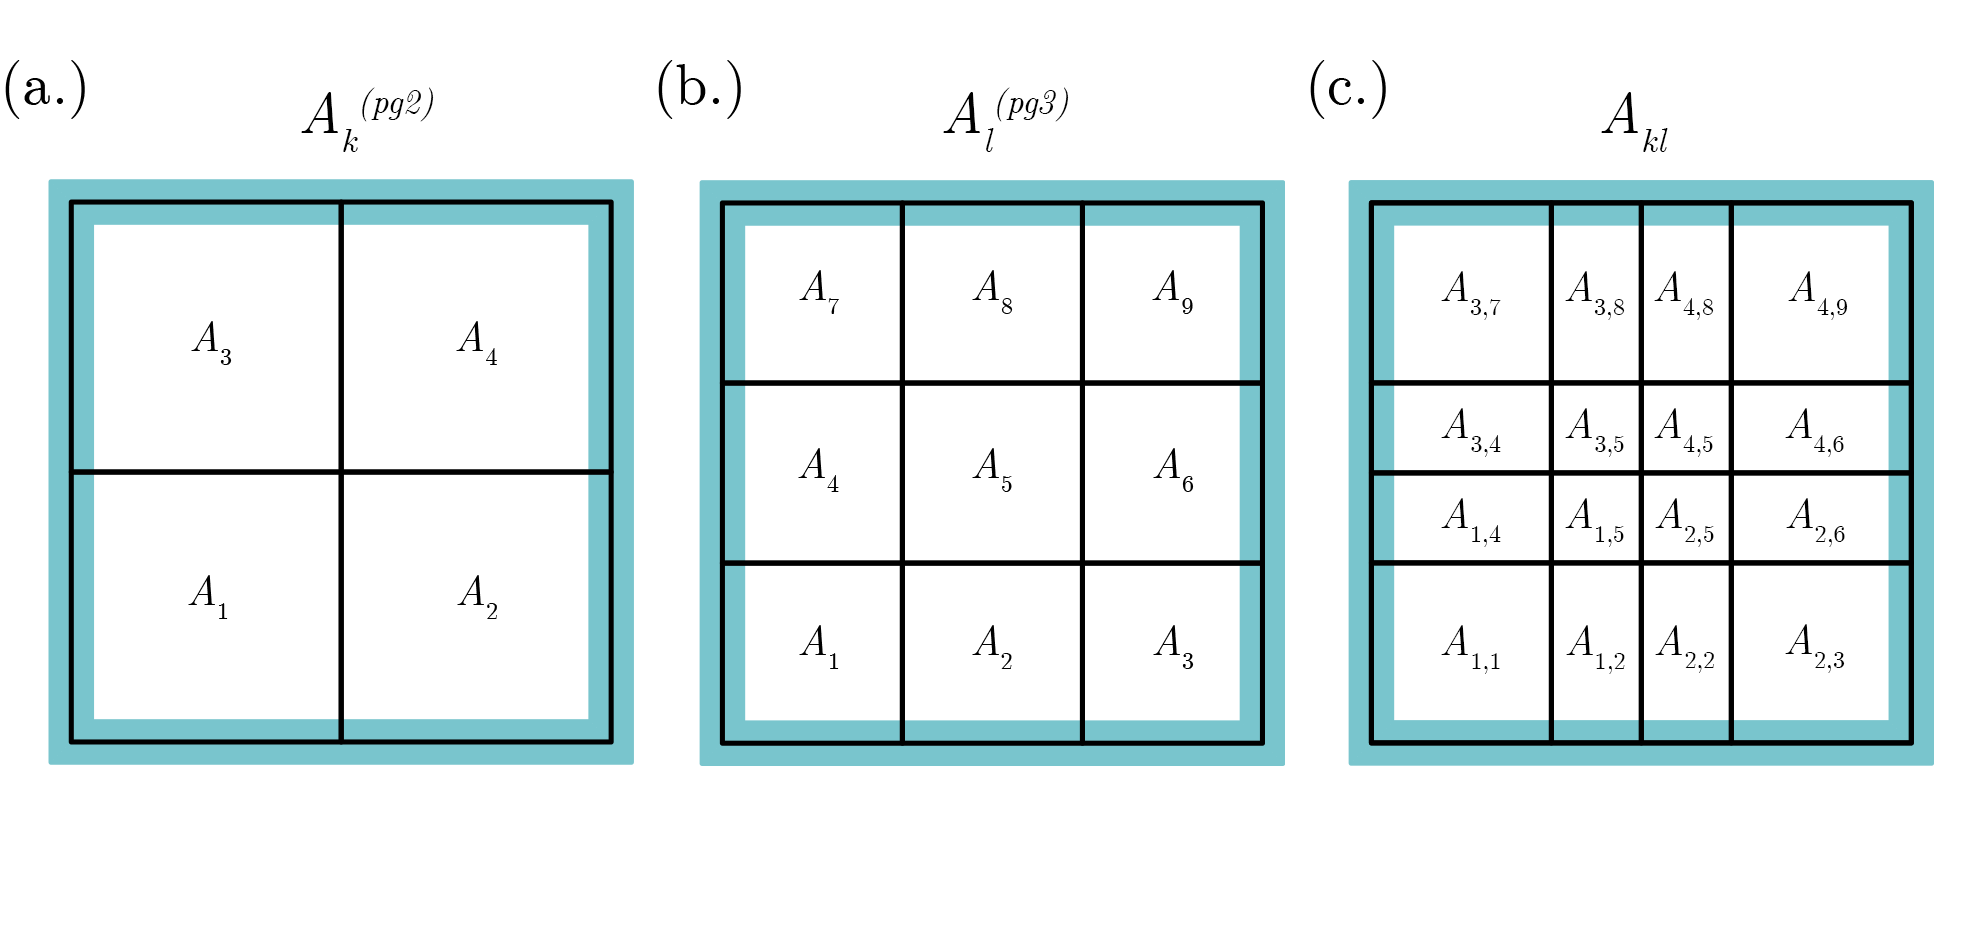
\includegraphics[width=30pc,angle=0]{chapter5/area-schematic.png}\\
\end{center}
\caption{Indices notation for (a) the $pg2$ grid, (b) the $pg3$ grid and (c) their exchange grid.}
\label{fig:area-schematic}
\end{figure}

Denote the known cell averaged values of dry pressure-level thickness and mixing ratio $\overline{\Delta p}^{(pg3)}$ and $\overline{m}^{(pg3)}$, respectively. We consider a particular layer and for simplicity drop the layer subscript. The same procedure is applied to each layer in a column. The unknowns we would like to compute are the cell-averaged values of the same quantities on the physics grid; $\overline{\Delta p}^{(pg2)}$ and $\overline{m}^{(pg2)}$, respectively. The dry pressure level thickness integrated over the $k$'th physics grid cell is given by
\begin{equation}
\label{eq:p}
\overline{\Delta p}^{(pg2)}_k=\frac{1}{\Delta A^{(pg2)}_k}\sum_{\ell=1}^{nc^2}\left<\delta p\right>_{k\ell},
\end{equation}
where $\left< \delta p\right>_{k\ell}$ is the dry mass in a layer over overlap area $A_{k\ell}$. It is computed by integrating a high-order (2D polynomial of degree 2) reconstruction of pressure-level thickness in each CSLAM cell over the overlap area $A_{k\ell}$
\begin{equation}
\label{eq:pg3dp}
\left< \delta p\right>_{k\ell}=\int_{A_{k\ell}}\left[ \sum_{i+j\le 2}{\mathcal{P}}^{(ij)}_\ell x^{i}y^{j}\right] dA.
\end{equation}
The reconstruction coefficients ${\mathcal{P}}^{(ij)}_\ell$ in CSLAM cell $\ell$ are computed from the cell average pressure level thicknesses on the CSLAM grid $\overline{\Delta p}^{(pg3)}$ and the numerical integration over overlap areas is done by line-integrals. The details of that are given in \cite{LNU2010JCP} and not repeated here.

The average tracer mass per unit area on the physics grid is given by
\begin{equation}
\label{eq:mp}
\overline{m\Delta p}^{(pg2)}_k=\frac{1}{\Delta A^{(pg2)}_k}\sum_{\ell=1}^{nc^2}\left< m\delta p\right>_{k\ell},
\end{equation}
where $\left< m\delta p\right>_{k\ell}$ is the tracer mass over $A_{k\ell}$ resulting from integrating a high-order reconstruction of $\Delta p$ and $m$ combined using the approach outlined in Appendix B of \cite{NL2010JCP} over the overlap area $A_{k\ell}$
\begin{equation}
\label{eq:mp2}
\left< m\delta p\right>_{k\ell}=\int_{A_{k\ell}}\left[ \overline{\Delta p}_\ell^{(pg3)}\sum_{i+j\le 2}{\mathcal{M}}^{(ij)}_\ell x^{i}y^{j}+{\overline{m}}_\ell^{(pg3)}\sum_{i+j\le 2}{\widetilde{{\mathcal{P}}}}^{(ij)}_\ell x^{i}y^{j}\right] dA,
\end{equation}
where ${\widetilde{{\mathcal{P}}}}^{(00)}_\ell={\mathcal{P}}^{(00)}_\ell-\overline{\Delta p}^{(pg3)}_\ell$ and ${\widetilde{{\mathcal{P}}}}^{(ij)}_\ell={\mathcal{P}}^{(ij)}_\ell$ for $i,j>0$, and ${\mathcal{M}}^{(ij)}_\ell$ are the reconstruction coefficients for the mixing ratio in CSLAM cell $A^{(pg3)}_\ell$. A shape-preserving limiter is applied to the reconstruction of mixing ratio $m$ \citep{BJ1989} and not $\Delta p$. This way of combining the reconstruction function for $\Delta p$ and $m$ in \eqref{eq:mp2} ensures that a constant mixing ratio is preserved (consistency), tracer mass is conserved, linear-correlations are preserved and tracer shape-preservation is retained. The mixing ratio on the physics grid is then
\begin{equation}
{\overline{m}}^{(pg2)}_k=\frac{\overline{\left( m\Delta p\right)}^{(pg2)}_k}{\overline{\Delta p}^{(pg2)}_k},
\end{equation}
where $\overline{\Delta p}^{(pg2)}_k$ is given in \eqref{eq:p}. 

Perhaps surprisingly a much more challenging problem is to map tracer increments (or state) from the physics grid to the CSLAM grid while retaining important properties such as mass-conservation, consistency, and correlation preservation. Why this mapping problem is challenging is explained in detail in Section \ref{sec:why} after having defined important properties for mapping physics increments/tendencies.
\subsubsection{Mapping tracer increments from $A^{(pg2)}$ to $A^{(pg3)}$ (physics to CSLAM grid)}\label{sec:pgtonc}
The increments from the parameterizations are computed on the physics grid. The tracer increment in physics grid cell $k$ is denoted $\overline{f}_k^{(pg2)}$ so that the updated mixing ratio on the physics grid is ${\overline{m}}^{(pg2)}_k+\overline{f}_k^{(pg2)}$. The problem is how to map $\overline{f}_k^{(pg2)}$ to the CSLAM control volumes, to obtain ${\overline{f}}^{(pg3)}$, satisfying the following constraints:
\begin{enumerate}
\item {\bf{Local mass-conservation}}: At a minimum total physics mass forcing on an element computed on the physics grid should equal the element physics mass forcing on the CSLAM grid
\begin{equation}
{\overline{f}}_k^{(pg2)}{\overline{\Delta p}}^{(pg2)}_k\Delta A_k^{(pg2)}=\sum_{\ell=1}^{nc^2}\left[{\overline{\Delta p}}^{(pg3)}_\ell {\overline{f}}^{(pg3)}_\ell\Delta A_{k\ell}\right],
\end{equation}
where $\overline{\Delta p}^{(pg2)}_k$ is the pressure level thickness in physics grid cell $k$ and similarly for $\overline{\Delta p}^{(pg3)}$. We enforce a more local constraint in which only mass-increments overlapping with a particular CSLAM cell contributes to the mass-increment in that CSLAM cell.
\item {\bf{Local shape-preservation in mixing ratio}}: The increments mapped to the CSLAM grid and added to the previous CSLAM state should not produce values smaller than the updated physics grid mixing ratios, ${\overline{m}}^{(pg2)}_k+\overline{f}_k^{(pg2)}$, or values smaller than the existing CSLAM mixing ratios that overlap with physics grid cell $A_\ell$
\begin{equation}
\label{eq:min}
\overline{m}^{(pg3)}_\ell+{\overline{f}}^{(pg3)}_\ell \ge \overline{m}^{(min)}_k=\min \left( {\overline{m}}^{(pg2)}_k+{\overline{f}}_k^{(pg2)},\left\{ {\overline{m}}_{k\ell} |\ell=1,nc^2\right\} \right),
\end{equation}
where
\begin{equation}
\label{eq:moverlap2}
\overline{m}_{k\ell}=\frac{\left< m\delta p_{k\ell}\right> }{\left< \delta p_{k\ell}\right>}.
\end{equation}
The numerator and denominator in \eqref{eq:moverlap2} are defined in \eqref{eq:pg3dp} and \eqref{eq:mp2}, respectively. In particular this means that an increment, when mapped to the $pg3$ grid, should not drive the state negative (described in detail below as the `negativity' problem).

A similar definition apply for maxima
\begin{equation}
\label{eq:max}
{\overline{m}}^{(pg3)}_\ell+{\overline{f}}^{(pg3)}_\ell \le \overline{m}_k^{(max)}=\max \left( {\overline{m}}^{(pg2)}_k+\overline{f}_k^{(pg2)},\left\{ {\overline{m}}_{k\ell} |\ell=1,nc^2\right\} \right),
\end{equation}
\item {\bf{Linear correlation preservation}}: The physics forcing must not disrupt linear tracer correlation between species on the CSLAM grid \citep[see, e.g., ][]{LT2011QJR}, i.e. if two tracers are linearly correlated and the physics increment preserves linear correlations on the physics grid then the tracer increment on the CSLAM grid must not disrupt linear correlations.
\item {\bf{Consistency}}: A non-zero constant mixing ratio increment from physics, $cnst$, on the physics grid, $\overline{f}_k^{(pg2)}=cnst$ $\forall k$, must result in the same (constant) forcing on the CSLAM grid, $\overline{f}_\ell^{(pg3)}=\overline{f}_k^{(pg2)}=cnst$ $\forall \ell$.
\end{enumerate}
To motivate the algorithm that will simultaneously satisfy 1-4 it is informative to discuss how `standard' mapping algorithms will violate one or more of the constraints:
\subsubsection{Why `conventional' conservative remapping will not work}\label{sec:why}
It is helpful to analyze in detail why conventional remapping can not satisfy properties 1-4 above. Assume that one remaps the mass-increments in exactly the same way as the mapping of mixing ratio state from the CSLAM grid to the physics grid described in section \ref{sec:nctopg}. That is, replace $m$ with $f$ and map from physics grid to the CSLAM grid instead of the other way around. Denote the mapped mass-increment $\widetilde{\overline{f\Delta p}}^{(pg3)}$ and due to the properties of the mapping algorithm the mass-increment is conserved, linear correlation between mass-increments are conserved and shape in mass-increment is preserved. The problems arise when converting from mass to mixing ratio.
\paragraph{Conserve mass but not consistency} 
If ones uses the known pressure-level thickness on the CSLAM grid ${\overline{\Delta p}}^{(pg3)}_k$ to convert from mass-increment to mixing-ratio increment
\begin{equation}
\label{eq:convert1}
\overline{m}^{(pg3)}_k=\frac{\widetilde{\overline{f\Delta p}}^{(pg3)}_k}{{\overline{\Delta p}}^{(pg3)}_k},
\end{equation}
a constant mixing ratio increment is not conserved. Basically the constant increment mapped to the CSLAM grid and converted to mixing ratio increment through \eqref{eq:convert1} will, rather than being constant, reflect the spurious discrepancy between $\widetilde{\overline{\Delta p}}^{(pg3)}_k$ and ${\overline{\Delta p}}^{(pg3)}_k$, where $\widetilde{\overline{\Delta p}}^{(pg3)}_k$ is the pressure-level thickness mapped from the $pg2$ grid to the $pg3$ grid. That said, mass will be conserved since the dynamical core state has ${\overline{\Delta p}}^{(pg3)}_k$ (unless the increment drives the mixing ratio negative - described in detail below). 
\paragraph{Consistent but not mass-conserving} 
Rather than converting to mixing ratio using ${\overline{\Delta p}}^{(pg3)}_k$, a constant increment can be preserved by using
\begin{equation}
\overline{m}^{(pg3)}_k=\frac{\widetilde{\overline{f\Delta p}}^{(pg3)}_k}{\widetilde{\overline{\Delta p}}^{(pg3)}_k},
\end{equation}
instead. But now mass-conservation is lost since, again, $\widetilde{\overline{\Delta p}}^{(pg2)}_k\ne {\overline{\Delta p}}^{(pg2)}_k$. This issue is similar to the mass-wind inconsistency found in specified dynamics applications \citep[e.g.][]{JKLSBCRE2001QJR,L2009LNCE}. 

\paragraph{The `negativity' problem and linear correlations} 
Even if one could derive a reversible map for mapping ${\overline{\Delta p}}^{(pg2)}$ from the physics grid to the CSLAM grid, there could still be problems if the increment drives the mixing ratios negative (or overshooting occurs) on the CSLAM grid. This can easily happen for tracers, such as cloud liquid amount and cloud ice amount, that are zero in most of the domain and non-zero in localized areas/points (where there are clouds). We refer to this as the `negativity problem'. This problem is depicted schematically in Figure~\ref{fig:alg-schematic}. Consider a single element of CSLAM control volumes, containing only a single cell with mixing ratio $1.0$, and $0.0$ everywhere else ($\overline{m}^{(pg3)}_\ell$; Figure ~\ref{fig:alg-schematic}a). The mixing ratios are mapped to the $pg2$ grid using, for simplicity, the piecewise constant method where a constant value inside the $pg2$ cells is used during the integration over overlap cells ($\overline{m}^{(pg2)}_k$; Figure~\ref{fig:alg-schematic}b). Now consider the case in which physics removes all the mass from the physics cell $k$: $\overline{f}^{(pg2)}_k=-\overline{m}^{(pg2)}_k$ (Figure~\ref{fig:alg-schematic}c). The tracer increment is mapped from $pg2$ to $pg3$ using the piecewise constant method. Some of the non-zero increments are now in overlap areas where the original CSLAM grid cells have mixing ratio zero ($\overline{f}_{k\ell}$; Figure~\ref{fig:alg-schematic}d), and hence, the state is driven negative when adding the overlap increment to the CSLAM state (Figure~\ref{fig:alg-schematic}e).  This is referred to as the negativity problem although it can also happen for maxima.

\begin{figure}[t]
\begin{center}
\noindent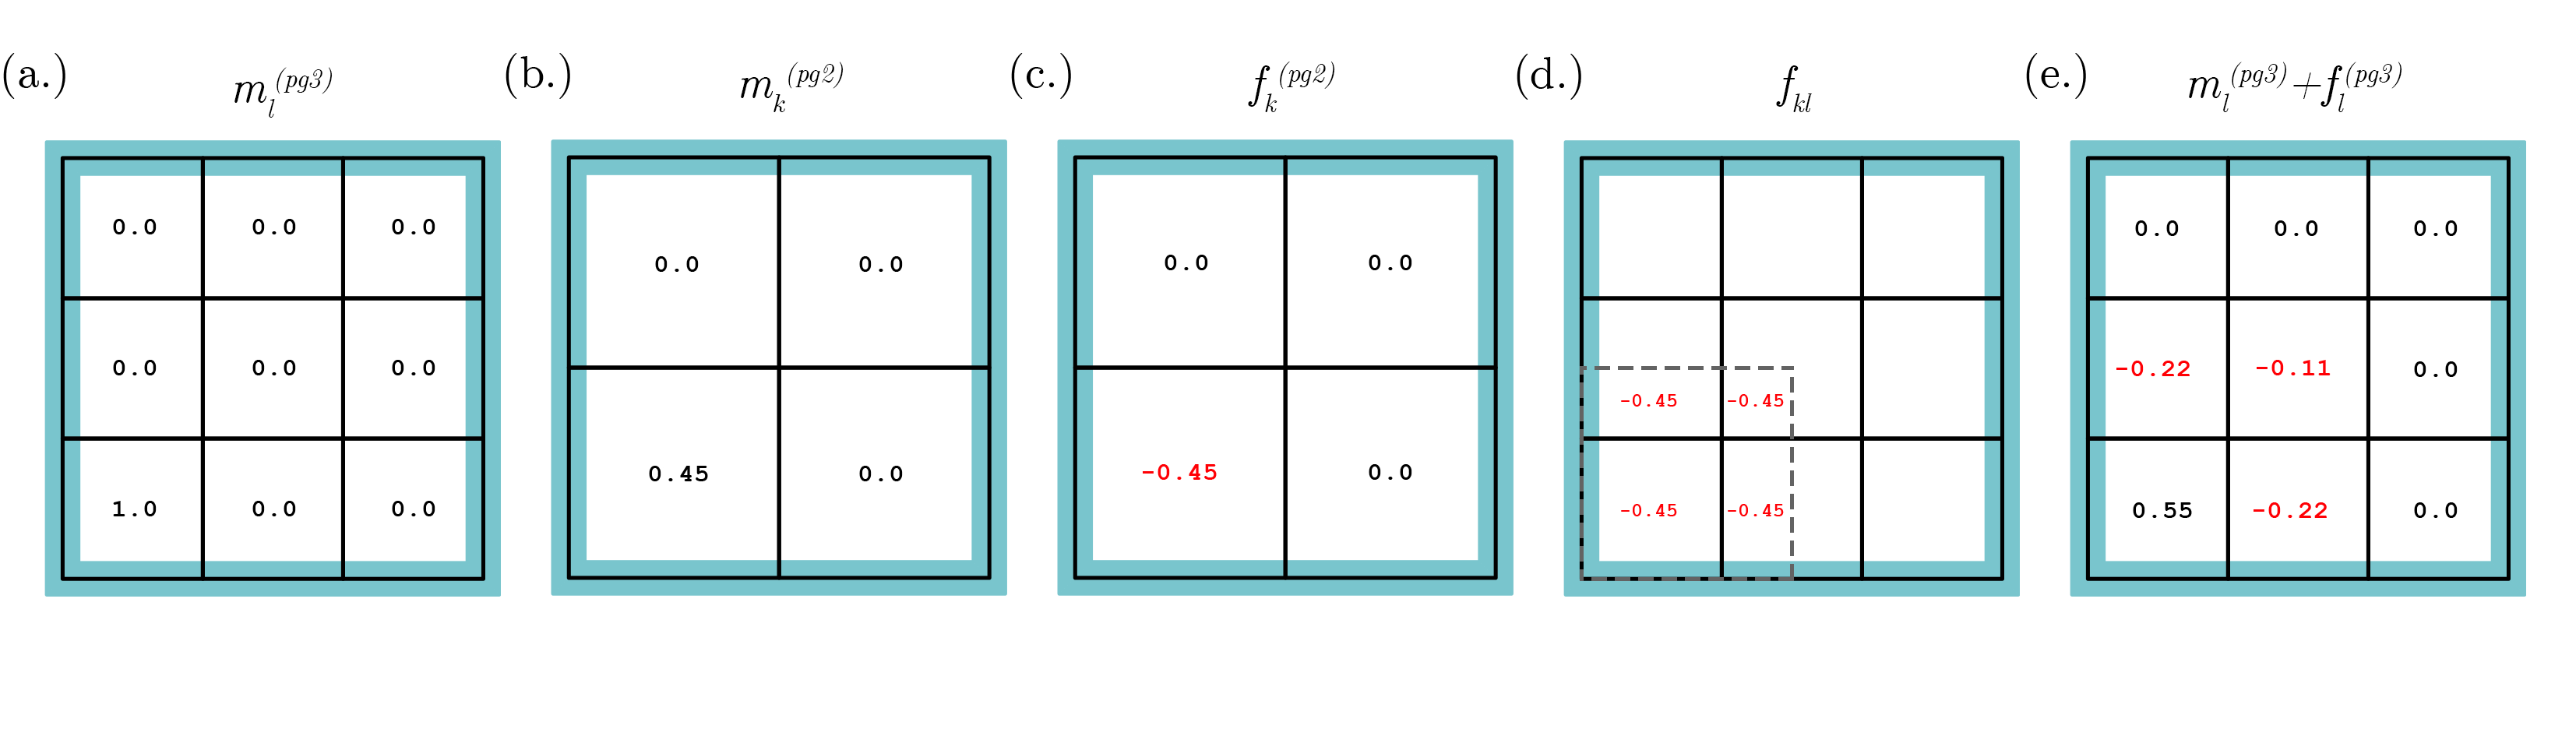
\includegraphics[width=40pc,angle=0]{chapter5/alg-schematic.png}\\
\end{center}
\caption{Schematic illustration of the `negativity problem' in a single element. (a.) Initial CSLAM tracer values, (b.) mapped to $pg2$, (c) produces a tracer increment on $pg2$, (d.) with negative increments on the exchange grid overlying CSLAM cells in (a) that were initially zero and (e) driving those mixing ratios negative.}
\label{fig:alg-schematic}
\end{figure}

The negativity issue could be avoided if one remaps the physics updated state instead of mapping increments/tendencies. In that case a shape-preserving filter will make sure that the state on the CSLAM grid is not negative (and does not overshoot). That said, if physics does not change the state and it is mapped back to the CSLAM grid then spurious tendencies (proportional to the errors introduced by mapping state from the CSLAM grid to the physics grid and back again) are introduced. Hence it is advantageous to map increments/tendencies since any reasonable algorithm will preserve a zero function.

As illustrated above a standard remapping method will NOT simultaneously satisfy 1-4 and hence a new algorithm has been derived.
\subsubsection{New tendency mapping algorithm}\label{sec:massfix}
The problem is how to map the mass-increment on the physics grid, ${\overline{f}}^{(pg2)}\Delta A^{(pg2)}$, to the CSLAM cells that overlap with $\Delta A^{(pg2)}$. To maintain shape-preservation, linear correlations and to avoid the negativity problem locally, it is advantageous to define a mass excess function on the exchange grid $\Delta m_{k\ell}^{(excess)}$. It is basically the maximum amount of mixing ratio that can be removed (in the case ${\overline{f}}^{(pg2)}<0$) without producing new minima in the exchange grid mixing ratio $m_{k\ell}$
\begin{equation}
\Delta m^{(excess)}_{k\ell}=\overline{m}_{k\ell}-\overline{m}_k^{(min)},
\end{equation}
where $\overline{m}_{k\ell}$ is defined in \eqref{eq:moverlap2}. So the maximum amount of mass that we can be removed from the exchange grid cells that span physics grid cell $A_k$ without violating the shape-preservation constraint (\eqref{eq:min} and \eqref{eq:max}) is
\begin{equation}
\sum_\ell \Delta m^{(excess)}_{k\ell}\overline{\Delta p}_{k\ell} \delta A_{k\ell}.
\end{equation}
If physics is designed not to remove more mass than available in $A_k$ (which should be the case for a carefully designed physics package) then it is guaranteed that
\begin{equation}
\label{eq:well-posed}
\sum_\ell \Delta m^{(excess)}_{k\ell}\overline{\Delta p}_{k\ell} \delta A_{k\ell}\ge {\overline{f}}^{(pg2)}\Delta p_k\Delta A^{(pg2)}.
\end{equation}
We distribute the physics mass-forcing (assuming ${\overline{f}}^{(pg2)}<0$) according to the mass excess in each overlap area by solving this equation for $\gamma_k$
\begin{equation}
\label{eq:mass-excess}
\Delta A_k^{(pg2)}\overline{\Delta p}_k^{(pg2)}{\overline{f}}^{(pg2)}=\gamma_k \sum_\ell \Delta m^{(excess)}_{k\ell}\overline{\Delta p}_{k\ell} \delta A_{k\ell},
\end{equation}
and add mass increment (which in this case is negative)
\begin{equation}
\label{eq:mass-incr}
\gamma_k \Delta m^{(excess)}_{k\ell}\overline{\Delta p}_{k\ell} \delta A_{k\ell},
\end{equation}
to the $\ell$th CSLAM cell state ${\overline{m}}^{(pg3)} \overline{\Delta p}^{(pg3)}_\ell \Delta A^{(pg3)}_\ell$. This process is repeated for all physics cells. Note that this problem is a well-posed, i.e. $\gamma_k>0$, since physics will not remove more mass than is locally available \eqref{eq:well-posed}. The way in which the mass-forcing is distributed to the CSLAM cells using the excess function insures that the negativity problem is avoided. Mass is conserved by design and shape-preservation is obtained by using the excess function.

If the physics increment is positive (assuming ${\overline{f}}^{(pg2)}>0$) we define a `lack' function
\begin{equation}
\Delta m^{(lack)}_{k\ell}=\overline{m}_{k\ell}-\overline{m}^{(max)},
\end{equation}
and solve
\begin{equation}
\label{eq:mass-lack}
\overline{\Delta p}_k^{(pg2)}{\overline{f}}^{(pg2)}\Delta A_k^{(pg2)}=\gamma_k \sum_\ell \left[ \Delta m^{(lack)}_{k\ell}\overline{\Delta p}_{k\ell} \delta A_{k\ell}\right],
\end{equation}
for $\gamma_k$ and follow the same procedure as for mass excess. Since positive and negative forcing is treated in exactly the same way, linear correlations are preserved. Note how the definition of the excess/lack function insures linear correlation preservation; for example, if one would prevent negative values and not do anything about overshoots then linear correlations would not be preserved since the minima and maxima are not treated in the same way.

While the above algorithm satisfies properties 1-4 in section \ref{sec:pgtonc}, it is not a high-order algorithm in terms of formal accuracy. This is illustrated in Figure \ref{fig:mapping} (row 3) where a smooth analytical tendency \citep[approximate spherical harmonic of order 32 and azimuthal wave number 16; ][]{J1999MWR}
\begin{equation}
\label{eq:Y32}
f^{(pg2)}=\frac{1}{2}+\frac{1}{2}\cos(16\lambda)\sin(2\theta)^{16},
\end{equation}
where $(\lambda,\theta)$ is latitude-longitude, is mapped from $pg2$ to $pg3$ grid using this algorithm assuming $m^{(pg3)}_\ell=0, \quad \forall \ell$. The errors in the mapping are not always aligned with large gradients in the analytical function as would be expected for a `traditional' interpolation algorithm. The errors are maximum on the order of 60$\%$. To reduce errors we therefore perform a higher-order pre-allocation of tendencies that is not mass-conserving but satisfies properties 2,3, and 4 in Section \ref{sec:pgtonc}.

\begin{figure}[t]
\begin{center}
\noindent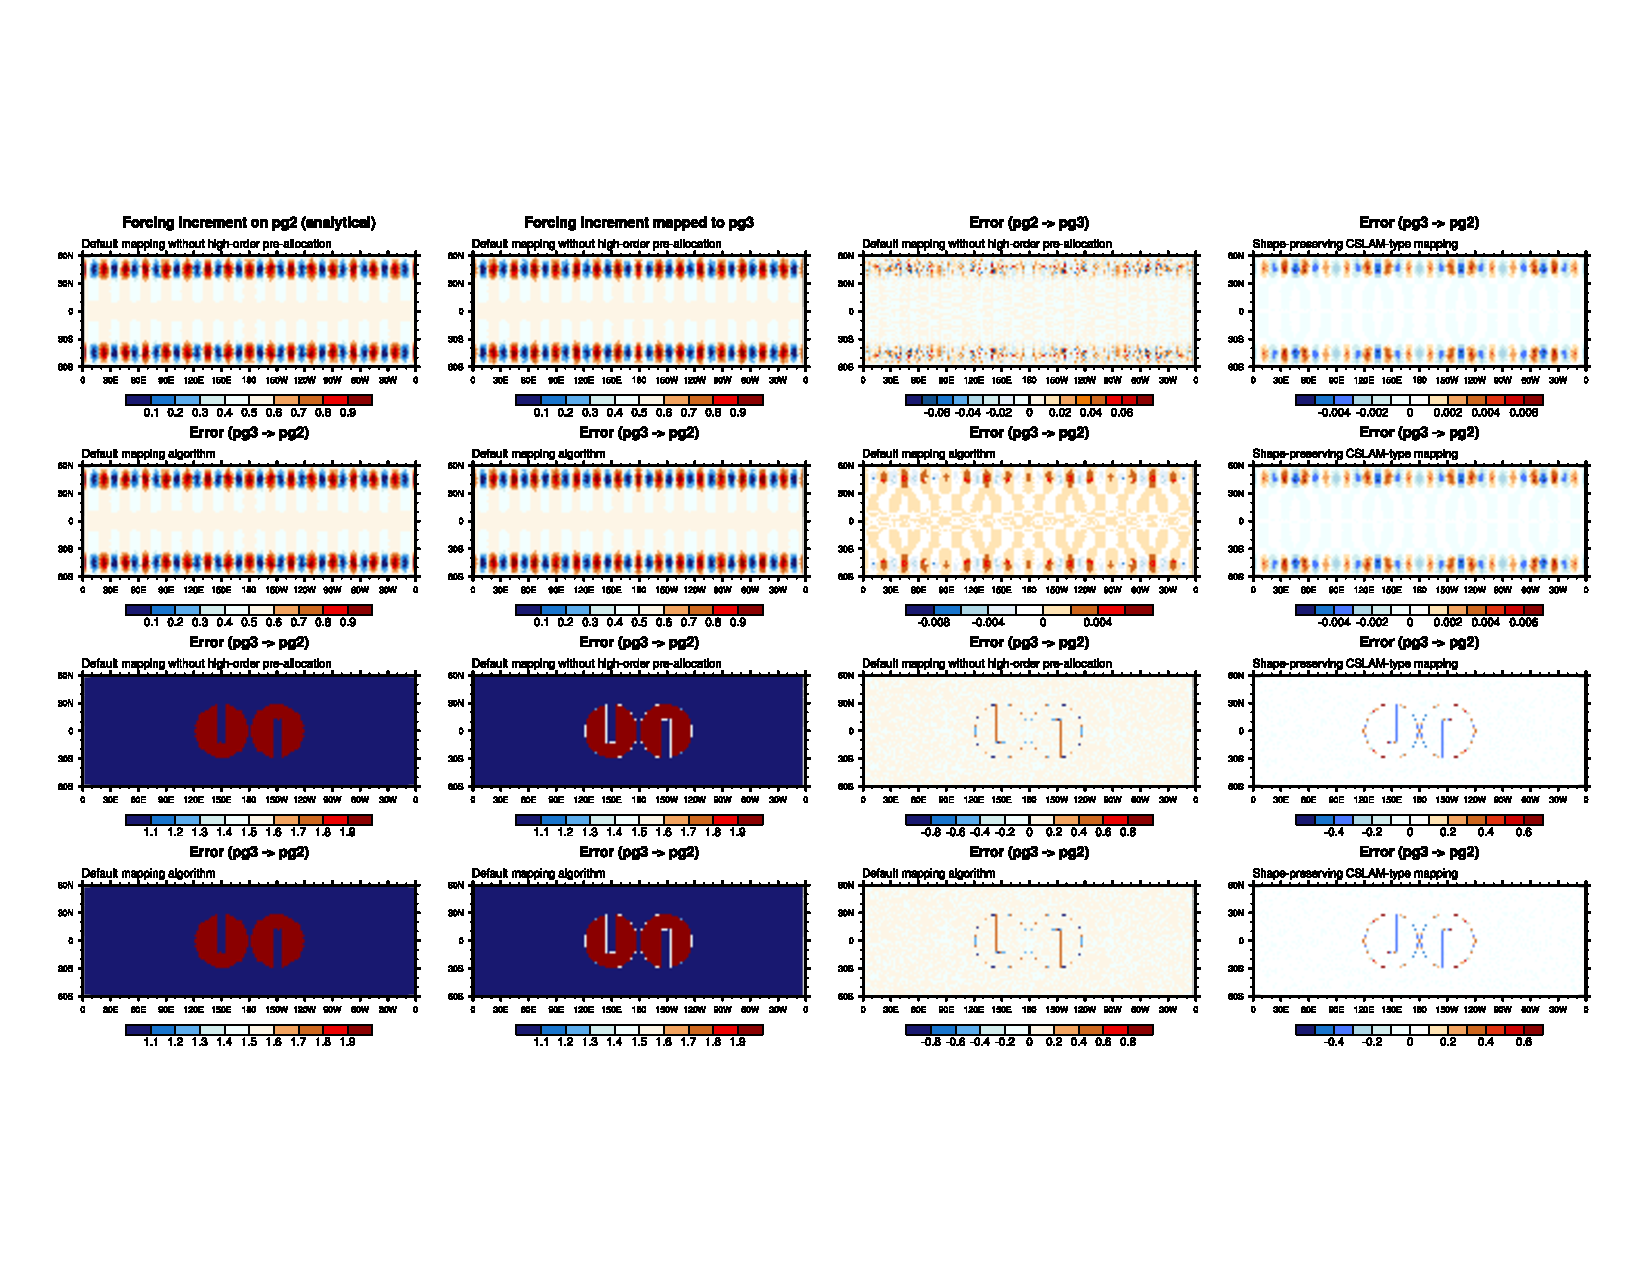
\includegraphics[width=40pc,angle=0]{chapter5/mapping.pdf}\\
\end{center}
\caption{Mapping of idealized functions from $pg2$ (column 1) to $pg3$ (columns 2) and errors (column 3) using the new tendency algorithm only (row 1 and 3) and new tendency algorithm with the high-order pre-allocation (row 2 and 4). Column 4 shows the errors in mapping the same distributions from  $pg3$ to $pg2$ using traditional remapping (CSLAM technology).}
\label{fig:mapping}
\end{figure}

\subsubsection{High-order (non-conservative) pre-allocation of tracer tendencies}
A high-order tracer mass increment in overlap area $A_{k\ell}$ can be computed using the following formula
\begin{equation}
\label{eq:mp3}
\left< f\delta p\right>_{k\ell}=\int_{A_{k\ell}}\left[ \overline{\Delta p}_\ell^{(pg3)}\sum_{i+j\le 2}{\mathcal{F}}^{(ij)}_k x^{i}y^{j}+{\overline{f}}_k^{(pg2)}\sum_{i+j\le 2}{\widetilde{{\mathcal{P}}}}^{(ij)}_\ell x^{i}y^{j}\right] dA,
\end{equation}
where $\mathcal{F}^{(ij)}_k$ is the forcing increment reconstruction coefficients in the $k$th physics grid cell and ${\overline{f}}_k^{(pg2)}$ is the average physics increment in the $k$th physics grid cell. Note that we are using the known dry pressure reconstruction coefficients on the $pg3$ grid instead of reconstructing sub-grid-scale pressure variations from the physics grid cell averaged values. We can do that since the dry pressure is not modified by physics. This highlights the importance of a dry-pressure formulation of the dynamical core when separating physics and dynamics grids \citep{LetAl2018JAMES}. If the physics forcing is constant then $\left< f\delta p\right>_{k\ell}$ exactly equals $\left<\delta p\right>_{k\ell}$ from \eqref{eq:pg3dp}; in other words, the mapping is designed to be reversible in dry pressure. The physics increment in terms of mixing ratio change is given by
\begin{equation}
\label{eq:pg3fq}
\overline{f}_{k\ell}=\frac{\left< f\delta p\right>_{k\ell}}{\left<\delta p\right>_{k\ell}},
\end{equation}
where the denominator is given by \eqref{eq:pg3dp}.

Shape-preservation, as defined by \eqref{eq:min} and \eqref{eq:max}, is enforced by eliminating under and overshoots on the exchange grid by modifying the forcing increment $\overline{f}_{k\ell}$ so that shape-preservation is not violated in the overlap areas{\footnote{In the computation of $\overline{m}_{k\ell}$ there can be small overshoots and undershoots (due to numerical integration errors) compared to the CSLAM cell average values $\overline{m}^{(pg3)}_\ell$ that it overlaps with so we set
\begin{equation}
\overline{m}_k^{(min)}=\min \left( \overline{m}_k^{(min)},\left\{ \overline{m}^{(pg)}_\ell)|\ell=1,nc^2\right\} \right)
\end{equation}}}
\begin{equation}
\overline{m}_k^{(min)} \le \overline{m}_{k\ell}+\widetilde{\overline{f}}_{k\ell} \le \overline{m}_k^{(max)}.
\end{equation}
While this algorithm preserves linear correlations, shape, and is consistent, is it not mass-conservative. Hence the remaining physics increment not allocated in the algorithm above is allocated using the new tendency algorithm described in Section \ref{sec:massfix}.

Combining the high-order pre-allocation algorithm with the new tendency algorithm (which in this case can also be considered as a mass-fixer that does not disrupt correlation-preservation, shape and consistency) leads to an order-of-magnitude reduction in mapping errors for a smooth function (see Figure \ref{fig:mapping} row 3 and 4) while full-filling the mass-conservation, shape-preservation, linear correlation and consistency  constraint. Mass and linear correlation preservation is illustrated in the baroclinic wave test with terminator chemistry test in Section \ref{sec:fkessler}. Shape-preservation and consistency is demonstrated in an idealized mapping test where a smooth function, see \eqref{eq:Y32}, and a slotted-cylinder \citep[see equation 12 in ][]{LSPT2012GMD} are mapped to/from the $pg2$ and $pg3$ grids. Since the background value in the mapping of the slotted-cylinder field is preserved the mapping algorithm is consistent. Since no new over- and undershoots are produced (particularly obvious in the mapping of the slotted cylinders) the mapping is shape-preserving. We also note that the mapping errors with the default algorithm (higher-order pre-allocation with new tendency algorithm) are similar to the errors in mapping the same field from $pg3$ to $pg2$ using traditional remapping with CSLAM technology (column 4 in Figure \ref{fig:mapping}).

\subsubsection{Model Configurations}\label{sec:config}

All simulations in this study are run on the Cheyenne supercomputer hosted at the NCAR-Wyoming Supercomputer Center \citep{AMPproj}. Three model component sets ({\em{compsets}}) in the Community Earth System Model, version 2.1 (CESM2.1; \url{https://doi.org/10.5065/D67H1H0V}) are chosen to carry out the objectives discussed in Section~\ref{sec:intro}. The least complex compset is a moist baroclinic wave test using a simple, Kessler microphysics scheme \citep[$FKESSLER$ compset;][]{LetAl2018JAMES}. The baroclinic wave setup is primarily used to evaluate the new mapping algorithms and their ability to preserve linear-correlations between two reactive tracers. The role of topography is investigated using a dry Held-Suarez configuration \citep[$FHS94$ compset;][]{HS1994} modified to include real world topography. H18 indicate that this configuration tends to have more grid-noise over steep terrain than in a more complex configuration using CAM, version 6 physics [CAM6; \url{https://ncar.github.io/CAM/doc/build/html/users_guide/index.html}], and is therefore a conservative choice for evaluating any change in grid imprinting between $pg3$ and $pg2$. 

To understand whether the resolved scales of motion are influenced by a coarser resolution physics grid, a suite of aqua-planet simulations \citep{NH2000ASL,MWO2016JAMES} are carried out over a range of spectral-element grid resolutions, using CAM6 physics ($QPC6$ compset). The aqua-planet is an ocean covered planet in perpetual equinox, with fixed, zonally-symmetric sea surface temperatures idealized after present day Earth \citep[$QOBS$ in][]{NH2000ASL}. While the dynamics time-step, $\Delta t_{dyn}$, varies with resolution according to a CFL criterion, there is no established standard for how the physics time-step, $\Delta t_{phys}$, should vary across resolutions. This is further complicated by several studies indicating a high sensitivity of solutions to $\Delta t_{phys}$ in CAM  \citep{WO2003QJR,W2013QJRMS,WETAL2015JAMES,HR2018JAMES}.

Here, a scaling for $\Delta t_{phys}$ across resolutions is proposed, based on results of the moist bubble test \citep{HR2018JAMES} using CAM-SE-CSLAM and detailed in Appendix~\ref{sec:app1}. The basis for the scaling is to alleviate truncation errors that arise in the moist bubble test when $\Delta t_{phys}$ is too large. The scaling is linear in grid-spacing,
\begin{equation}
\Delta t_{phys} = \Delta t_{phys,0} \times \frac{N_{e,0}}{N_e}~s,\label{eq:dt-scale}
\end{equation}
where $\Delta t_{phys,0}$ is taken to be the standard $1800 s$ used in CAM-SE-CSLAM at low resolution, $N_{e,0} = 30$ (equivalent to a dynamics grid-spacing of $111.2km$). $N_e$ refers to the horizontal resolution of the grid; each of the six panels of the cubed-sphere are divided into $N_e \times N_e$ elements. Throughout the paper, spectral-element grid resolutions are denoted by an $ne$ followed by the quantity $N_e$, e.g., $ne30$.

The only other parameter varied across resolutions modulates the strength of explicit numerical dissipation. The spectral element method is not implicitly diffusive, so fourth-order hyper-viscosity operators are applied to the state to suppress numerical artifacts. The scaling of the hyper-viscosity coefficients, $\nu$, across resolutions is defined as,
\begin{align}
\nu_T = \nu_{vor} &= 0.30\times \left(\frac{30}{N_e}1.1\times 10^5\right)^3\, \frac{m^4}{s}, \\
\nu_p = \nu_{div} &= 0.751\times \left(\frac{30}{N_e}1.1\times 10^5\right)^3\, \frac{m^4}{s},
\label{eq:hypervis}
\end{align}
where subscripts $T,~vor,~p,~div$ refer to state variables the operators are applied to, temperature, vorticity, pressure and divergence, respectively. The exponent in equation~\eqref{eq:hypervis} reduces the coefficient by about\footnote{This is approximate. To reduce the coefficients by exactly an order of magnitude for each doubling of the resolution, the exponent should be $\frac{\ln{2}}{\ln{10}}\approx3.01029$, which it has been updated to in the most recent version of CESM2.1} an order of magnitude for each doubling of the resolution \citep[as in][]{LetAl2018JAMES}. No explicit dissipation of tracers (e.g., water vapor) is required since the semi-Lagrangian numerics in CSLAM are diffusive.

\subsection{Results}\label{sec:results}

\subsubsection{Mass Conservation and Linear-Correlation Preservation}\label{sec:fkessler}

To illustrate how different the solutions look using the coarser resolution physics grid, Figure~\ref{fig:baro} shows a snapshot of the cloud liquid field of the moist baroclinic wave test on day 10, in the $ne30pg3$ and $ne30pg2$ configurations. The cloud liquid fields show in detail clouds forming at wave fronts. As expected, the $pg2$ grid looks slightly coarser than $pg3$ due to its larger control volumes. Despite this, the details of the wave patterns look reasonably similar to one another.

\begin{figure}[t]
\begin{center}
\noindent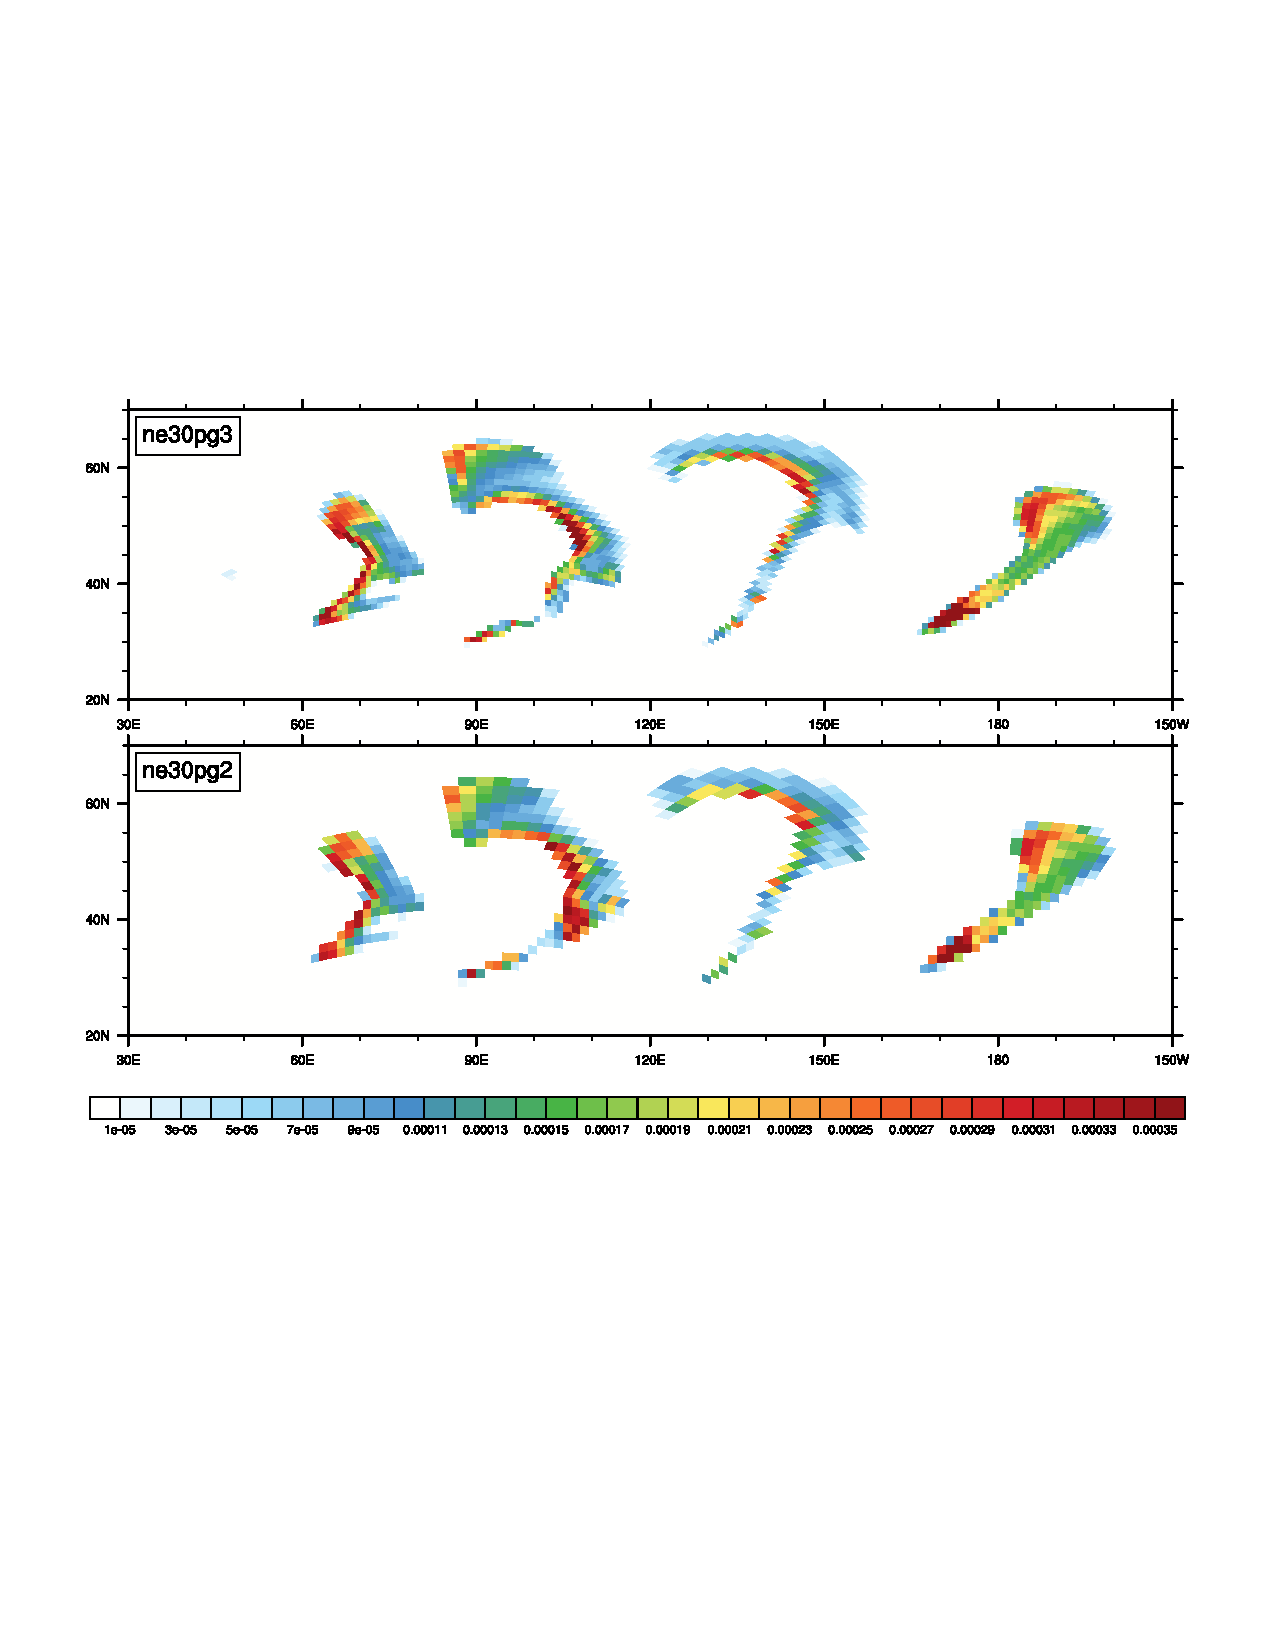
\includegraphics[width=25pc,angle=0]{chapter5/temp_CLDLIQ.pdf}\\
\end{center}
\caption{Snapshot of the cloud liquid field in kg kg$^{-1}$ near the $700 hPa$ level, on day 10 of the moist baroclinic wave test in the $ne30pg3$ and $ne30pg2$ configurations, displayed on the upper and lower panels, respectively. The fields are shown as a raster plot on their respective physics grids.}
\label{fig:baro}
\end{figure}

The models ability to preserve linear correlations is assessed using the idealized Terminator "Toy" Chemistry test \citep{LCLVT2015GMD,LTOUNGK2017MWR}. The tests consists of two reactive species undergoing photolysis as they are are advected over the terminator line. The flow field is provided by the moist baroclinic waves test. The model is initialized with species such that their weighted sum $Cl_y$ is a constant, i.e., $Cly = Cl + 2Cl_2 = 4\times10^{-6}$ kg kg$^{-1}$. If linear-correlations are preserved, than the column integrated weighted sum of the species, $\langle CLy \rangle$, is constant.

\begin{figure}[t]
\begin{center}
\noindent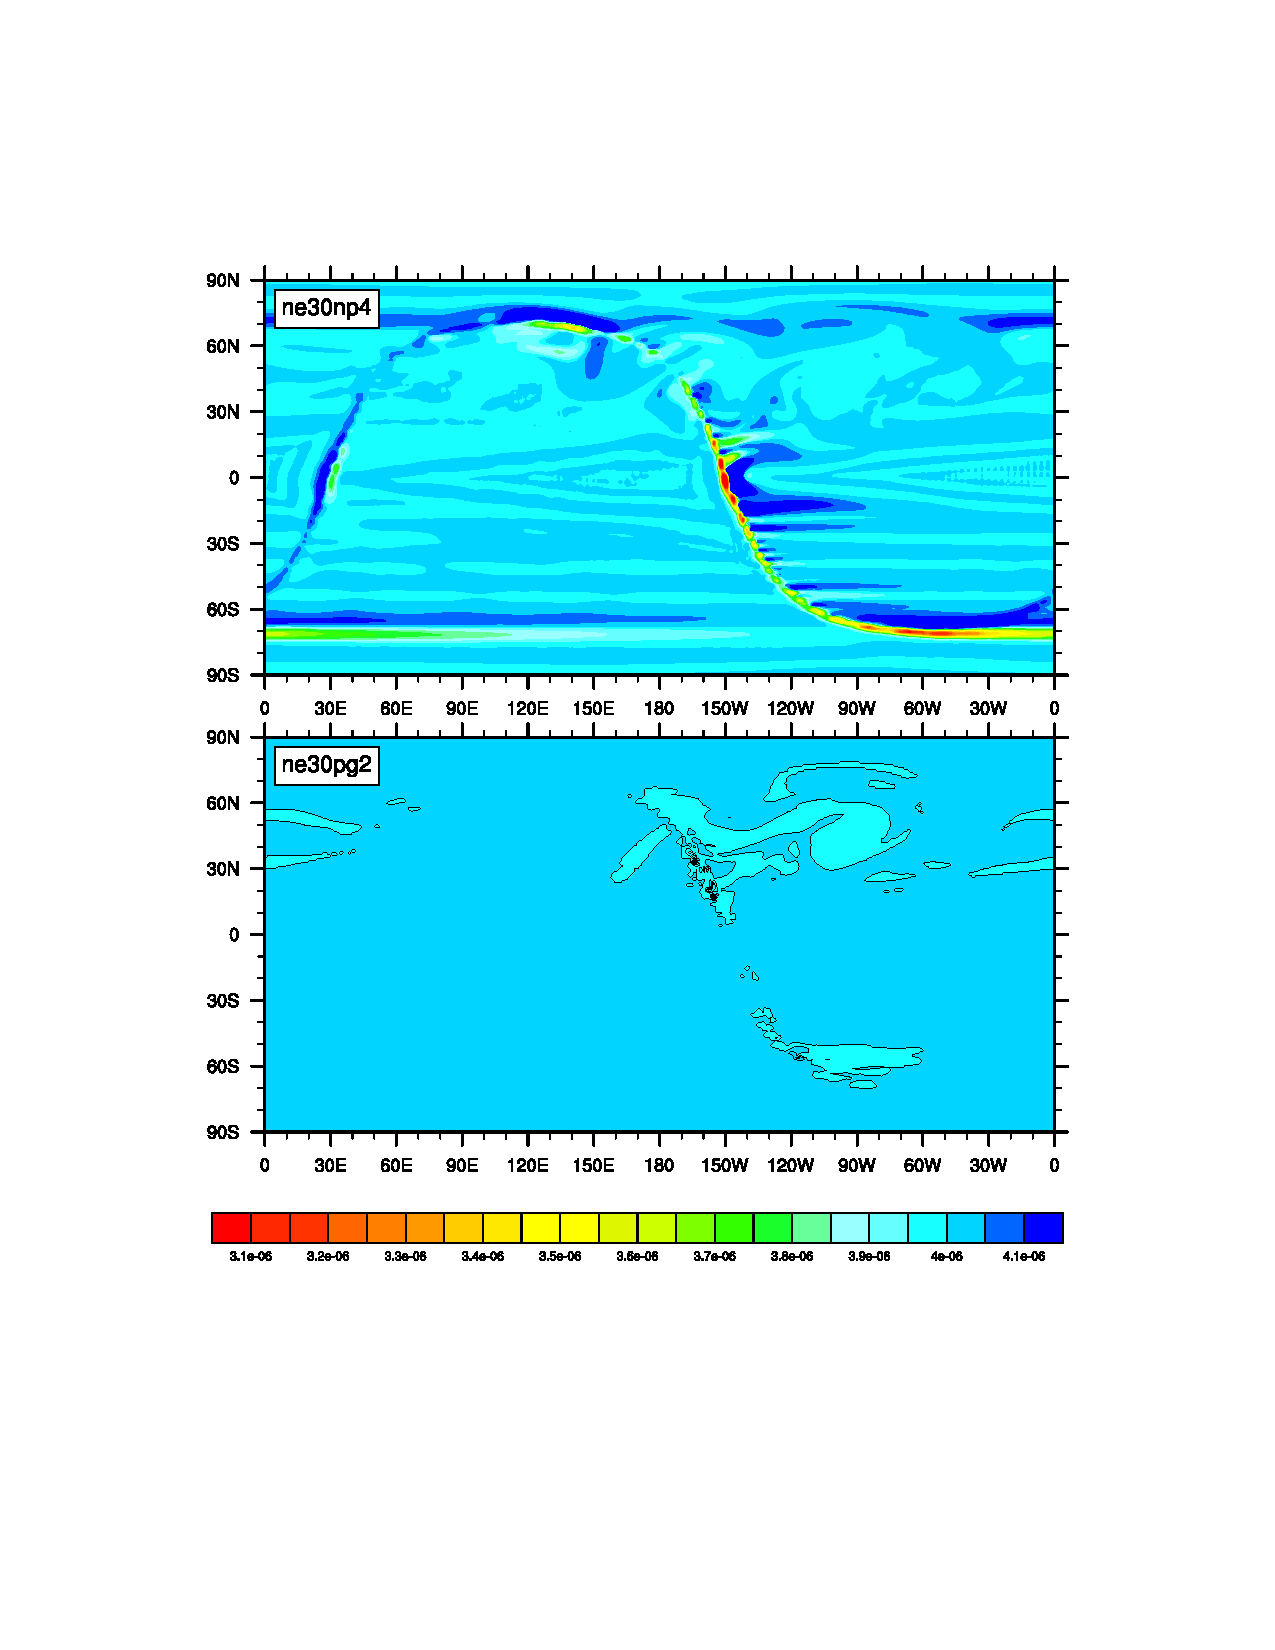
\includegraphics[width=20pc,angle=0]{chapter5/temp_terminator.pdf}\\
\end{center}
\caption{$\langle CLy \rangle$ in kg kg$^{-1}$ on day 15 of the moist baroclinic wave test in the $ne30np4$ and $ne30pg2$ configurations, displayed on the upper and lower panels, respectively. The lower panel has a single contour level of 3.999E-6 kg kg$^{-1}$ corresponding to a relative error of $0.025\%$.}
\label{fig:terminator}
\end{figure}

H18 had shown that in the $ne30pg3$ configuration, $\langle CLy \rangle$ on day 15 of the terminator test is everywhere $4\times10^{-6}$ kg kg$^{-1}$, to within machine precision. While the $pg3$ to $pg2$ mapping algorithm in theory preserves linear correlations to machine precision, we found larger than round-off errors in $pg2$, likely due to $if$-logic with machine dependent thresholds in the implementation of the algorithm. Figure~\ref{fig:terminator} shows $\langle CLy \rangle$ on day 15 in the $ne30pg2$ configuration, which has a minimum value of $3.99936\times10^{-6}$ kg kg$^{-1}$, corresponding to a maximum relative error of $0.016\%$. For comparison, another terminator test is performed with the equivalent dynamics grid resolution using CAM-SE ($ne30np4$), in which tracers are advected using the spectral element method. The maximum relative error in this configuration is $31.6\%$, three orders of magnitude greater error than the $ne30pg2$ configuration.

Tracer mass conservation is analyzed in a pair of $ne30pg2$ and $ne30pg3$ aqua-planet simulations, following the method of \cite{LW2019JAMES}. Energy and mass conservation due to a particular model process is assessed by model state I/O before and after each sub-process in the model. The loss of water vapor mass due to the mapping algorithms in the $ne30pg2$ configuration is estimated as $1.184$E$-16$ Pa per time-step, computed as the difference between the the column integrated, global mean climatological water vapor pressure increment on the physics grid and on the tracer grid. This small error is effectively zero to within machine precision, and similar to an equivalent calculation in the $ne30pg3$ simulation of $2.171$E$-17$ Pa per time-step, which contains no mapping errors since the physics and tracer grids coincide. Negligible mapping error in the $ne30pg2$ configuration is primarily a result of solving equations~\eqref{eq:mass-excess},\eqref{eq:mass-lack} for $\gamma_k$ to circumvent the `negativity' problem. Re-running the $ne30pg2$ aqua-planet simulation without this mass fixer, e.g., through setting $\gamma_k=1$ and $\Delta m^{(excess)}_{k\ell} = \overline{m}_{k\ell}$ in the mass increment \eqref{eq:mass-incr}, results in a spurious loss of water vapor mass of $2.424$E$-07$ Pa per time-step; the mass fixer is necessary for conserving tracer mass in $ne30pg2$. 


\subsubsection{Grid Imprinting}\label{sec:hs94}

Flow over topography can result in significant grid imprinting using the spectral element method \citep[][H18]{gmdd-8-4623-2015}. Figure \ref{fig:fhs-contours} shows the results of the Held-Suarez with topography simulations. The middle panel is the vertical pressure velocity, $\omega$, averaged over two years, over the Andes and Himalayan region at two different levels in the mid-troposphere, using the $ne30pg3$ grid. The fields are displayed as a raster plot on the physics grid, so that individual extrema, which characterize the flow over the Andes between about $10^\circ-20^\circ$ S, may be identified as spurious. Near the foot of the Himalayas, between about $20^\circ-30^\circ$ N, there are parallel stripes of extrema aligned with the mountain front that appear to be spurious $2\Delta x$ oscillations.

\begin{figure}[t]
\begin{center}
\noindent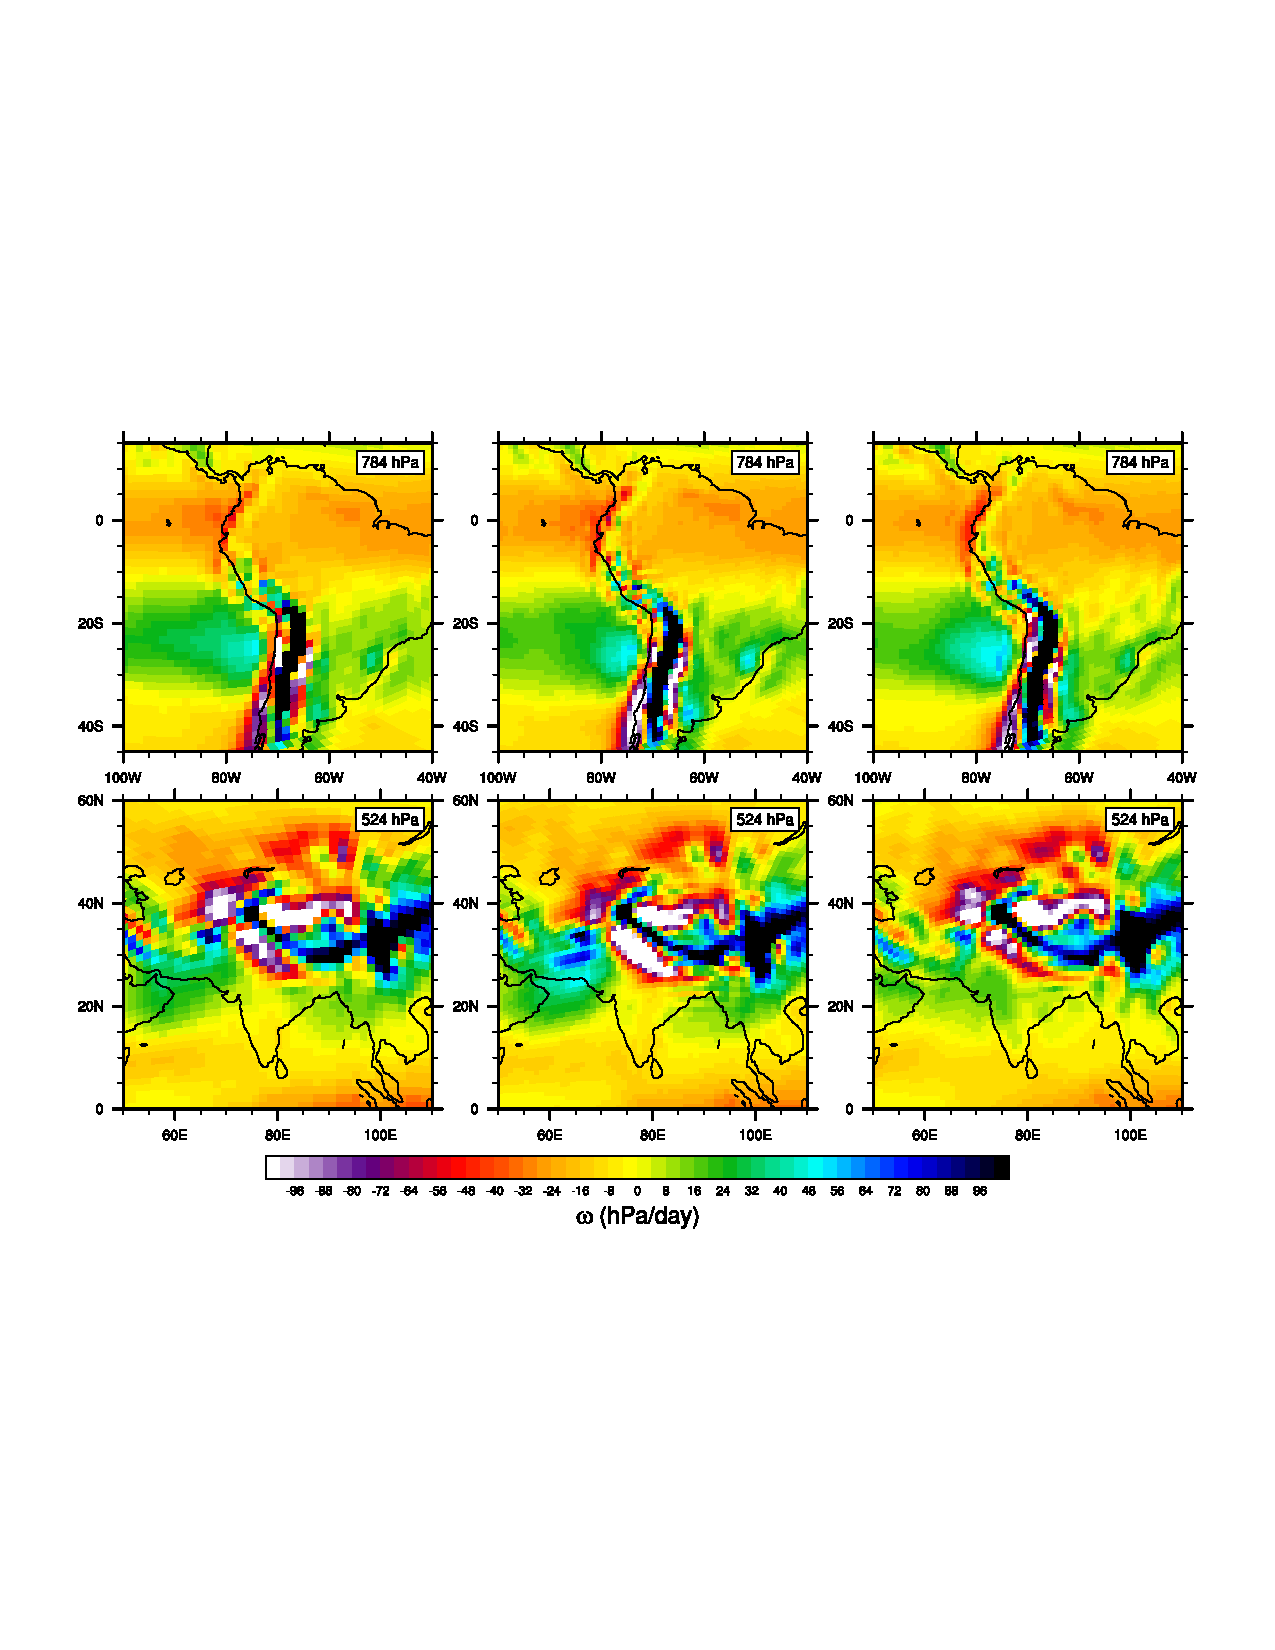
\includegraphics[width=30pc,angle=0]{chapter5/fhstopo_ne30pg2-v-ne30pg3-v-10Xnudiv.pdf}\\
\end{center}
\caption{Mean $\omega$ at two model levels in the middle troposphere, in a Held-Suarez configuration outfitted with real world topography. (Left) $ne30pg2$ (Middle) $ne30pg3$ and (Right) $ne30pg3$ with the divergence damping coefficient, $\nu_{div}$, increased by an order of magnitude. The $\omega$ fields are computed from a two-year simulation. The data are presented on a raster plot in order to identify individual grid cells}
\label{fig:fhs-contours}
\end{figure}

As discussed in H18, grid imprinting over mountainous terrain tends to occur in regions of weak gravitational stability, causing extrema to extend through the full depth of the troposphere as resolved updrafts and downdrafts. Thus, grid imprinting over mountains may be alleviated through increasing the divergence damping in the model. Figure \ref{fig:fhs-contours} (right panel) repeats the $ne30pg3$ simulation through increasing $\nu_{div}$ by an order of magnitude. The spurious noise over the Andes and the Himalayas are damped, and grid point extrema tend to diffuse into neighboring grid cells. The wavenumber-power spectrum of the kinetic energy due to divergent flow (Figure \ref{fig:fhs-div}) confirms that divergent modes are damped at higher wavenumbers (greater then 30), by about an order of magnitude relative to the default $ne30pg3$ simulation.

\begin{figure}[t]
\begin{center}
\noindent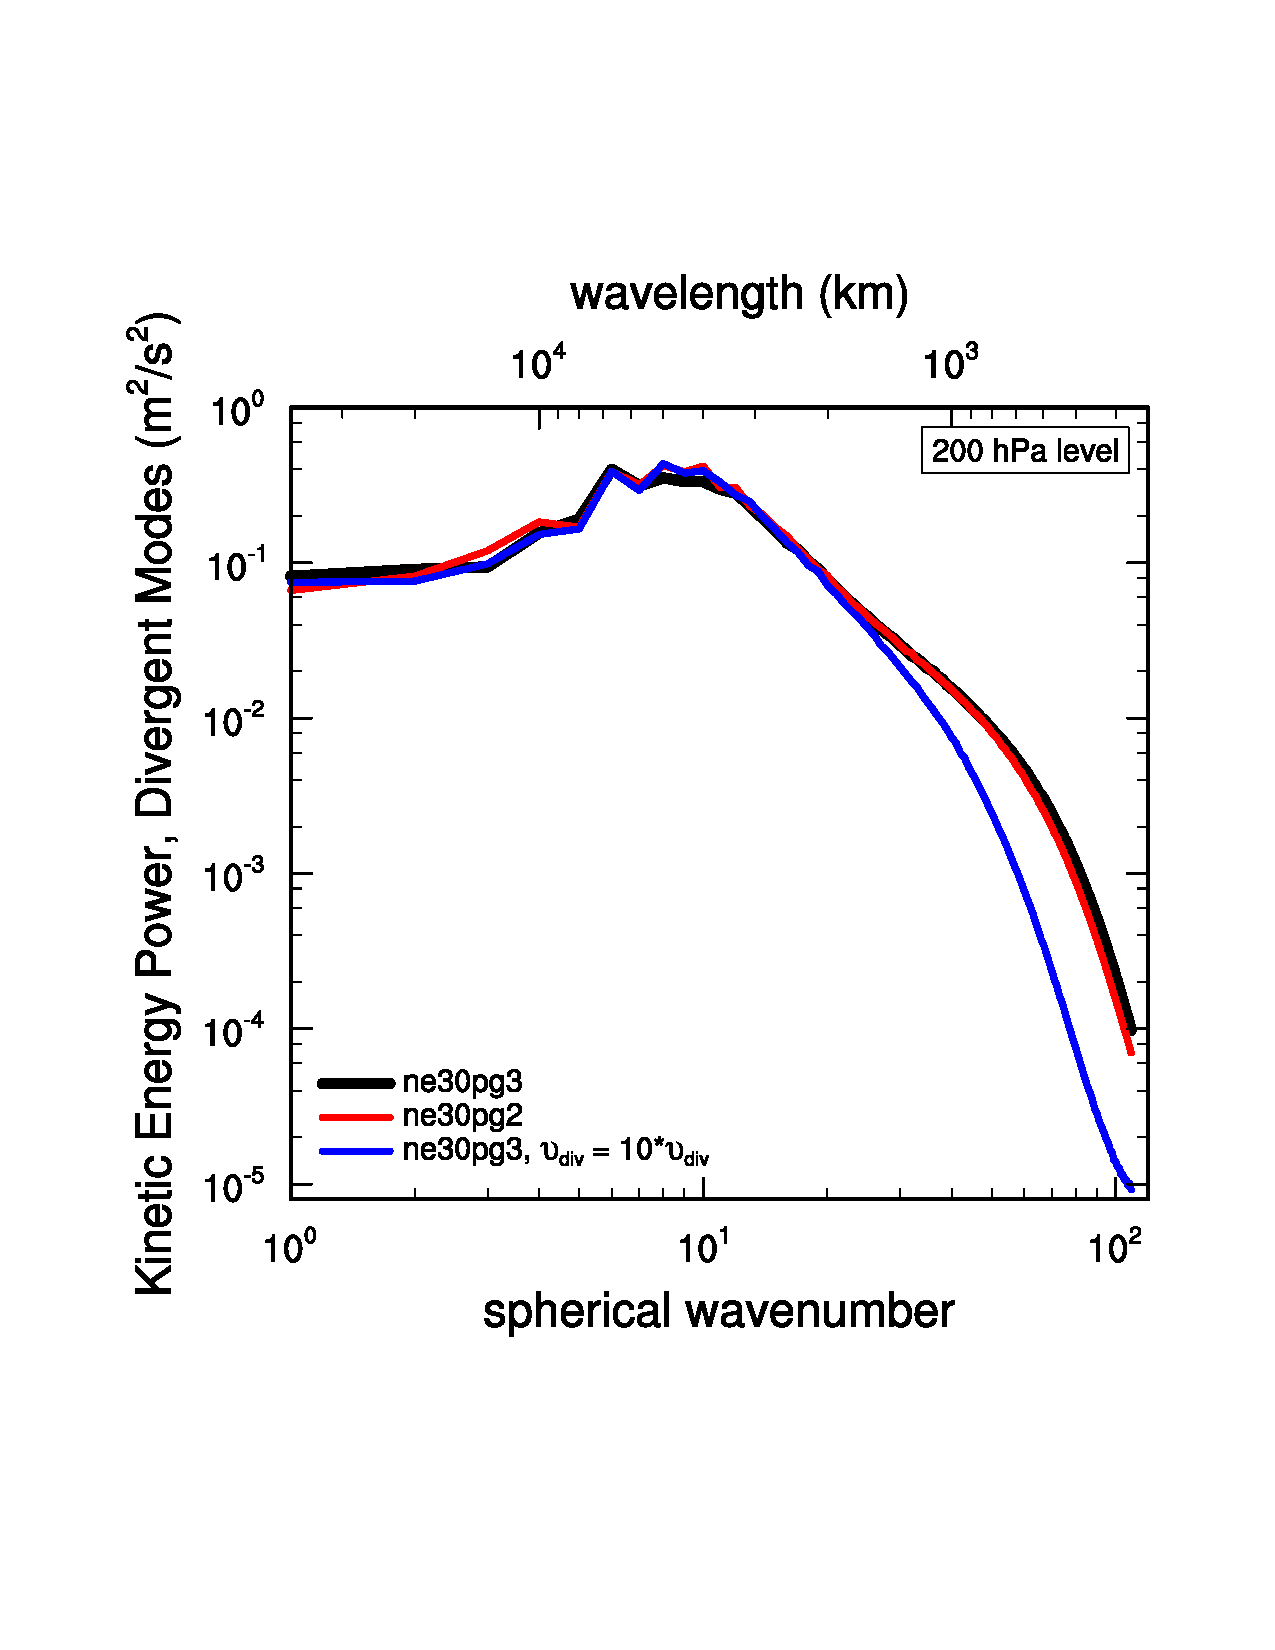
\includegraphics[width=20pc,angle=0]{chapter5/fhstopo_Divergence_ne30pg2-v-ne30pg3-v-10Xnudiv.pdf}\\
\end{center}
\caption{Kinetic energy power spectrum arising from divergent modes in $ne30pg3$, $ne30pg2$ and $ne30pg3$ with the divergence damping coefficient, $\nu_{div}$, increased by an order of magnitude, in the Held-Suarez with topography simulations. Spectra computed from five months of six-hourly winds.}
\label{fig:fhs-div}
\end{figure}

The $\omega$ field of the $ne30pg2$ simulation is provided in Figure \ref{fig:fhs-contours} (left panel). Grid cell extrema over the Andes is less prevalent than in the $ne30pg3$ simulation, as seen by the reduction in large magnitude $\omega$ (e.g., red grid cells). The spurious oscillations at the foot of the Himalayas appear to have been entirely eliminated. This improvement in grid imprinting is due to the consistent smoothness properties of the control volumes in the $pg2$ grid compared with the $pg3$ grid discussed in Section \ref{sec:intro}, and these results are consistent with our hypothesis. The divergent modes are marginally damped relative to $ne30pg3$ for wavenumbers greater than about 50, but are an order of magnitude larger than in the enhanced divergence damping $ne30pg3$ run (Figure \ref{fig:fhs-div}). From a scientific and model development perspective, the $pg2$ configuration is preferable to the $pg3$ configuration, since it eliminates grid imprinting without placing any additional constraints on $\nu_{div}$.

\subsubsection{Impact on Resolved Scales of Motion}\label{sec:aquaplanet}

Tropical regions are very sensitive to horizontal resolution, primarily due to the scale dependence of resolved updrafts and downdrafts at hydrostatic scales \citep{WETAL1997MWR,PG2006JAS,J2017JAMES,HR2017JCLIM,HR2018JAMES}. The vertical velocity of updrafts and downdrafts is related to the horizontal length scales of buoyancy the model is able to support. This can be demonstrated through a scale analysis of the Poisson equation \citep{JR2016QJRMS} valid for hydrostatic scales, showing that the ratio of the scale of $\omega$ at two resolutions, due to their respective buoyancies is,
\begin{equation}
\frac{\omega_{\Delta x_1}}{\omega_{\Delta x_2}} =  \frac{D_{\Delta x_2}}{D_{\Delta x_1}}~,\label{eq:w-scale}
\end{equation}
where $D_{\Delta x}$ is a characteristic buoyancy horizontal length scale for grid-spacing $\Delta x$ (hereafter referred to as the {\em{forcing scale}}), and it is presumed that the magnitude of the buoyancy and the vertical scale of the buoyancy is unchanged or compensating across the two resolutions. Equation~\eqref{eq:w-scale} indicates that the magnitude of the vertical velocity scales like the inverse of the forcing scale, which was verified in a simple moist bubble configuration using CAM-SE and the CAM finite-volume dynamical core \citep{HR2018JAMES}, as well as using CAM-SE-CSLAM as configured in the present study (Appendix~\ref{sec:app1}). It is by no means trivial that equation~\eqref{eq:w-scale} holds for the moist bubble test, since the scaling is derived from the dry anelastic equations.

In aqua-planet simulations using CAM-SE, the forcing scale is grid-limited, varying with resolution in the range of five to ten times the grid-spacing \citep{HR2018JAMES}. From equation~\eqref{eq:w-scale}, this grid-dependence explains why the updrafts and downdrafts are so sensitive to horizontal resolution. A grid-limited forcing scale is analogous to an effective resolution, which is the characteristic length scale below which the solution becomes contaminated by numerical artifacts, and the features are overly damped due to numerical dissipation. The effective resolution may be inferred from kinetic energy spectra as the wavenumber where the slope of the spectrum becomes steeper than the observationally determined slope \citep{S2011LNCSE}. In the CESM2 release of CAM-SE, this criterion occurs near wavenumber 60 \citep[see Figure 6 in][]{LetAl2018JAMES}, a length scale of about six times the grid spacing and overlapping with the estimated forcing scale.

When the physics and dynamics grids are of different resolutions, which grid determines the models characteristic forcing scale? The remainder of Section~\ref{sec:results} attempts to address this question using spectral element grids at low resolution (Section~\ref{sec:lores}), high resolution (Section~\ref{sec:hires}) and across all resolutions typical of present day climate models (Section~\ref{sec:allres}).

\paragraph{Low Resolution}\label{sec:lores} ~\\


The question posed above may be addressed through comparing $ne30pg2$, where $\Delta x_{phys} = 166.8km$ (hereafter $\Delta x$ is expressed as the average equatorial grid spacing), $\frac{3}{2}$ times larger than the dynamics grid spacing, $\Delta x_{dyn} = 111.2km$, to a simulation where both are equal to the physics grid spacing, $\Delta x_{dyn} = \Delta x_{phys} = 166.8 km$ ($ne20pg3$), and another simulation where both are equal to the dynamics grid spacing, $\Delta x_{dyn} = \Delta x_{phys} = 111.2 km$ ($ne30pg3$). The resolvable scales in the $ne30pg2$ solution are expected to be bounded by the $ne20pg3$ and $ne30pg3$ solutions. Although according to equation~\eqref{eq:dt-scale}, $\Delta t_{phys}$ for $ne20$ grids should be different from $ne30$ grids, here it is set to the $ne30$ value (see Table~\ref{table:grids-lo}) in order to reduce the differences between the three configurations, and justified because lower resolution runs aren't very sensitive to this range of $\Delta t_{phys}$ (Figure~\ref{fig:pdf-dtphys}).

 \begin{table}
 \caption{$\Delta x$ and $\Delta t$ for the physics and dynamics in the low resolution simulations. $\Delta x$ is computed as the average equatorial grid spacing.}
 \centering
 \begin{tabular}{llcccc}
 \hline
 Grid name & $\Delta x_{dyn}$  & $\Delta t_{dyn}$ & $\Delta x_{phys}$  & $\Delta t_{phys}$ \\
 \hline
   {\tt{ne}}20{\tt{pg3}}  & 166.8km & 300s  & 166.8km & 1800s \\
   {\tt{ne}}30{\tt{pg2}}  & 111.2km & 300s  & 166.8km & 1800s \\
   {\tt{ne}}30{\tt{pg3}}  & 111.2km & 300s  & 111.2km & 1800s \\
 \hline
 \end{tabular}
 \label{table:grids-lo}
 \end{table}
 
\begin{figure}
\begin{center}
\noindent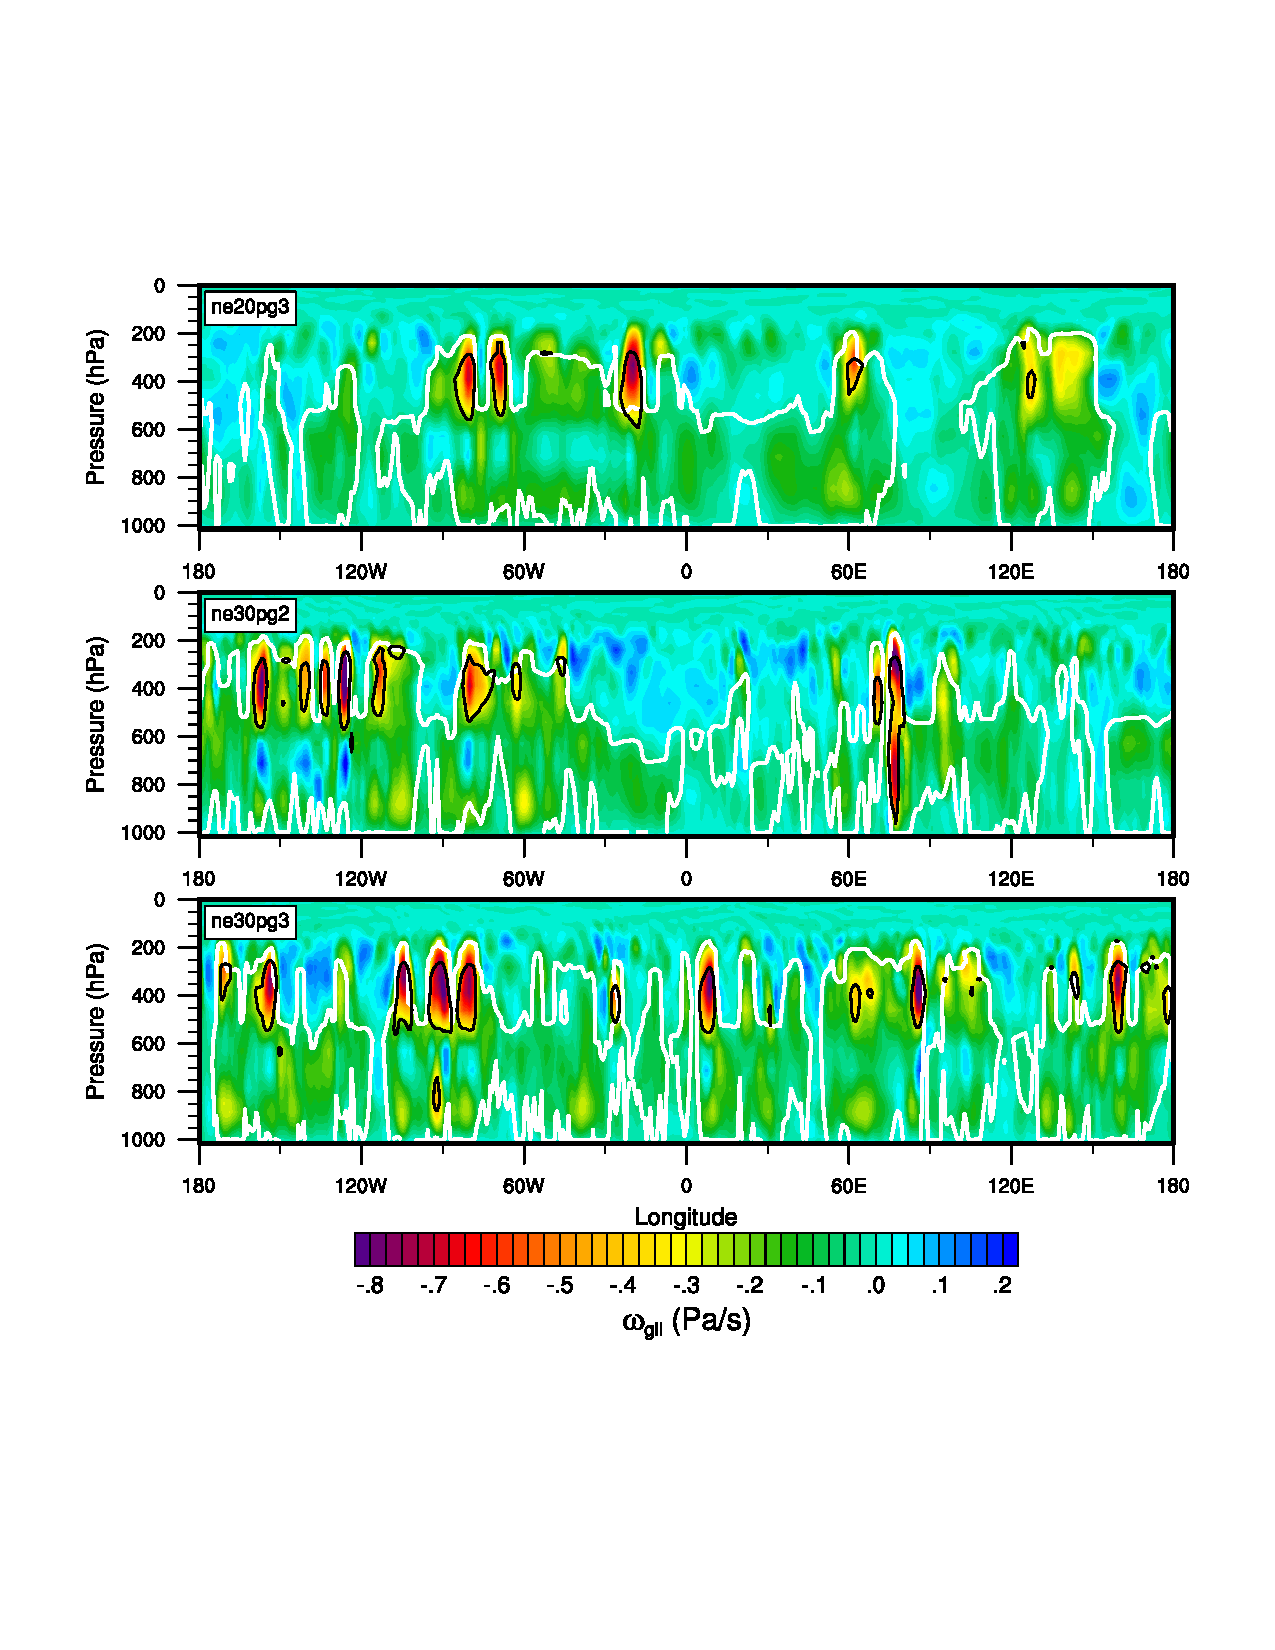
\includegraphics[width=30pc,angle=0]{chapter5/panel_transGLL.pdf}\\
\end{center}
\caption{Snapshots in the longitude-pressure plane of $\omega^{(gll)}$ through the ITCZ region in the $ne20pg3$, $ne30pg2$ and $ne30pg3$ configurations, in the upper, middle and lower panels, respectively. Black is the $\pm 15 K/day$ contour of the physics tendencies, and the white contour is the $0.0075 kg/m^2/s$ contour of the parameterized deep convective mass fluxes.}
\label{fig:transx}
\end{figure}

Figure~\ref{fig:transx} is a snapshot of the $\omega$ field in the Inter-Tropical Convergence Zone (ITCZ) in the pressure-longitude plane, in the three simulations. The $\omega$ field is overlaid with the $\pm 15 K/day$ contour of the physics temperature tendencies (black), which are primarily due to stratiform cloud formation. Since the component of $\omega$ due to buoyancy is determined by the physics temperature tendencies mapped to the GLL grid, the tendencies and $\omega$ are shown on the $GLL$ grid, $f_T^{(gll)}$ and $\omega^{(gll)}$, respectively. The white contour is intended to outline regions where the deep convection scheme is fairly active, set to the $0.0075 kg/m^2/s$ value of the convective mass fluxes (note the convective mass fluxes have not been mapped to the $GLL$ grid, and are instead shown on the $pg$ grid). The figure indicates that large regions of the ITCZ are comprised of upward $\omega$ that balance the warming due to compensating subsidence produced by the deep convection scheme. Much larger magnitude $\omega$ are comprised of resolved updrafts driven by the buoyancy of stratiform clouds, and resolved downdrafts due to evaporation of condensates produced by overlying clouds \citep{HR2018JAMES}. These large buoyancy stratiform clouds tend to form in the middle-to-upper troposphere due to detrainment of moisture from the deep convection scheme \citep{ZM1995AO}. 

It is not obvious from the snapshots in Figure~\ref{fig:transx} whether the length scales of the stratiform clouds, which are approximately equal to the models characteristic forcing scale, are any different across the three simulations. Analogous to determining the effective resolution \citep{S2011LNCSE}, the forcing scale may be inferred from the wave-number power spectrum of $f_T^{(gll)}$ as the maximum wavenumber prior to the steep, un-physical decline in power that characterizes the near-grid scale (hereafter $f_T^{(gll)}$ is referred to as the {\em{forcing}}). The wave-number power spectrum of the forcing in the middle-to-upper troposphere is shown in Figure~\ref{fig:pgXpanel-lores}a. Unlike kinetic energy spectra, the decline in power near the models effective resolution is more gradual, making it difficult to determine a characteristic forcing scale from the spectra. However, it is clear that the slope of the $ne20pg3$ spectrum begins to steepen at smaller wavenumbers than in the $ne30pg3$ spectra. Additionally, the $ne30pg2$ spectra is remarkably similar to the $ne30pg3$ spectra, for all wavenumbers. These spectra indicate that the characteristic forcing scale in the $ne30pg2$ and $ne30pg3$ simulations are similar, and that both are smaller than the $ne20pg3$ forcing scale. From equation~\eqref{eq:w-scale}, it is expected that the magnitude of the vertical motion is greater in both the $ne30pg2$ and $ne30pg3$ simulations.

\begin{figure}[t]
\begin{center}
\noindent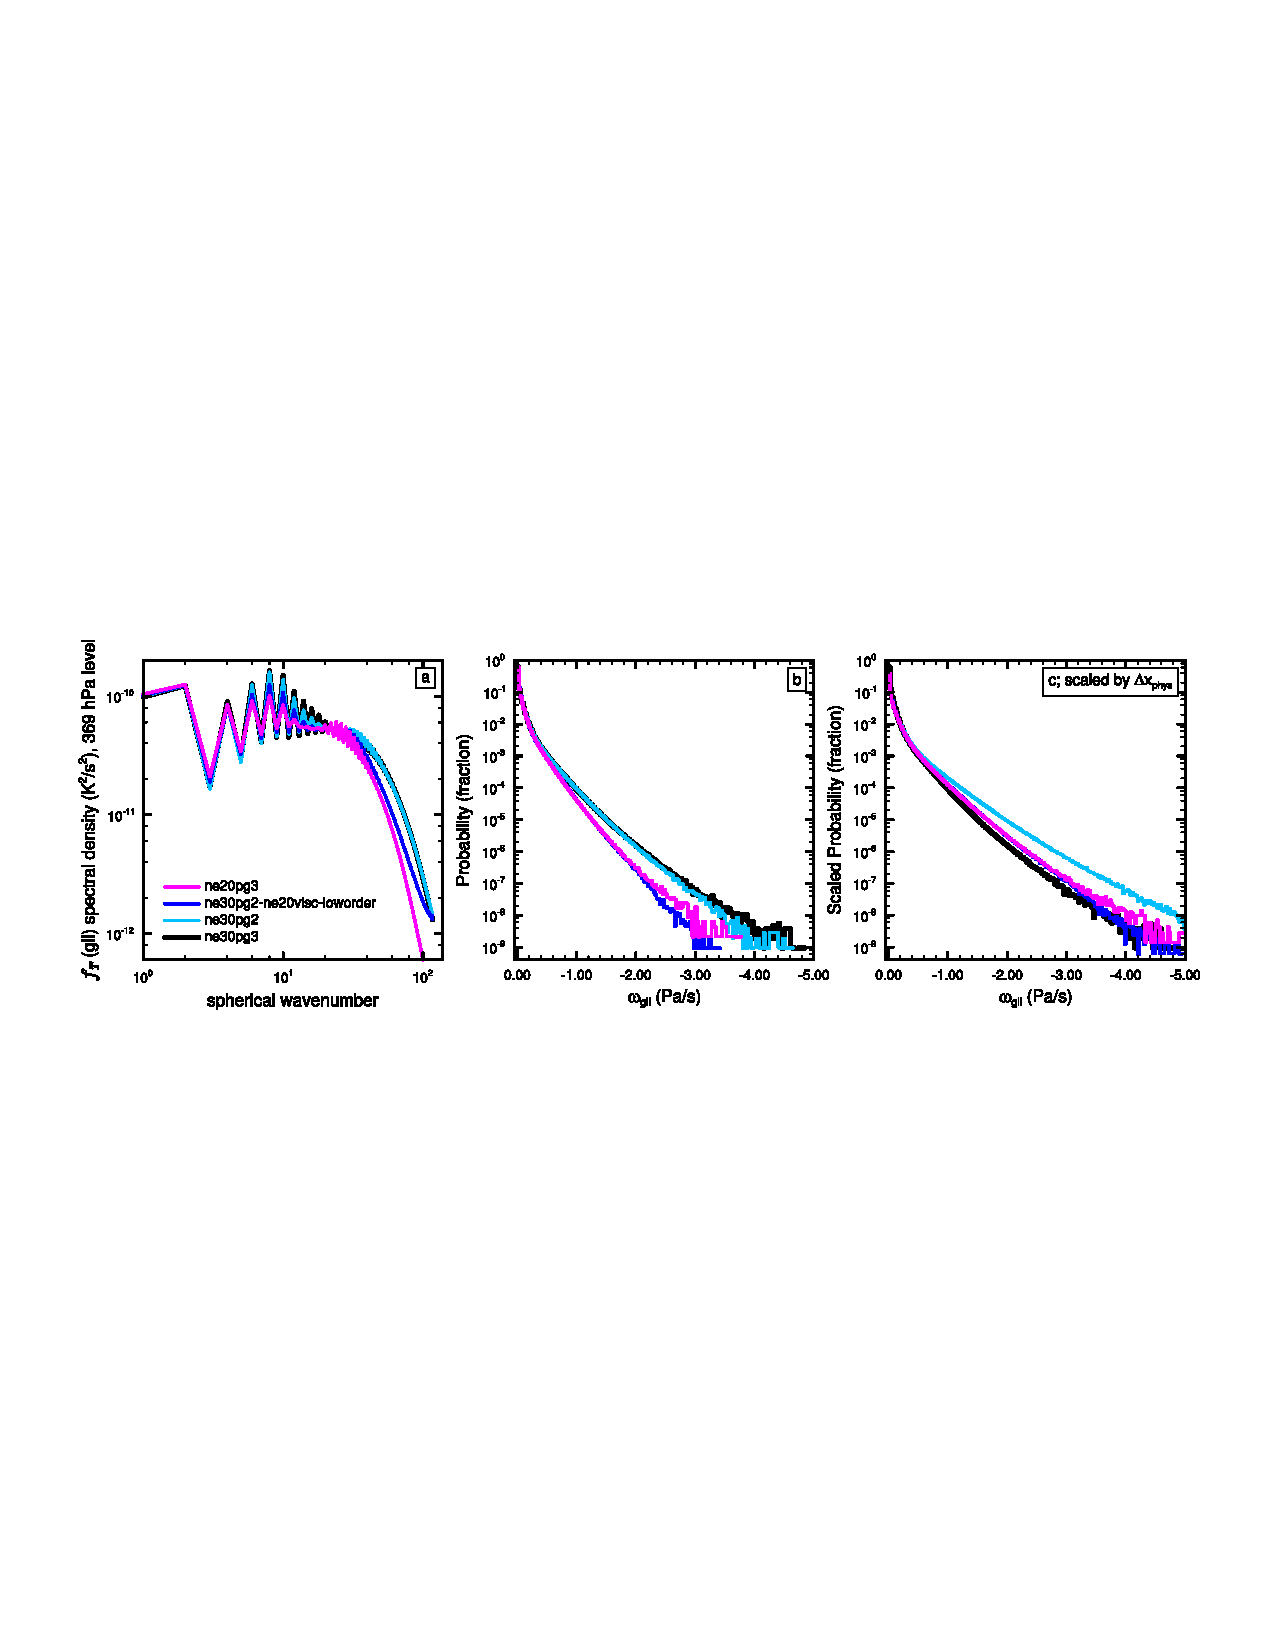
\includegraphics[width=40pc,angle=0]{chapter5/panel_ne20pg2-ne30pg2-ne30pg3.pdf}\\
\end{center}
\caption{(Left) Wavenumber-power spectrum of the temperature tendencies from the moist physics, near the 369 hPa level, (Middle) probability density distribution and (Right) the scaled probability density distribution of upward $\omega$ everywhere in the model. The scaled distributions are scaled to $ne30pg3$ using $\Delta x_{phys}$.}
\label{fig:pgXpanel-lores}
\end{figure}

The probability density function (PDF) of upward $\omega^{(gll)}$ everywhere in the simulations is shown in Figure~\ref{fig:pgXpanel-lores}b. Large magnitude $\omega^{(gll)}$ are more frequent in the $ne30pg2$ run, compared to $ne20pg3$, and the PDF is actually more similar to the $ne30pg3$ distribution, consistent with their similar forcing scales. This may be further illustrated through scaling the PDF's,
\begin{equation}
P_{s}(\omega) = \alpha \times P(\omega/\alpha),\label{eq:pdf}
\end{equation}
where $P_{s}(\omega)$ is the scaled PDF of $\omega$ and $\alpha$ is the ratio of $\omega$ to $\omega_{target}$, the $\omega$ associated with the target grid resolution, $\Delta x_{target}$. Making the assumption that the forcing scale is linear in $\Delta x$, then from equation~\eqref{eq:w-scale}, $\alpha = \Delta x_{target}/\Delta x$. The target resolution is taken here to be equal to the $ne30pg3$ grid resolution. 

If the forcing scale of $ne30pg2$ is in fact determined by $\Delta x_{phys}$, then one sets $\Delta x = \Delta x_{phys}$ in $\alpha$. This scaled PDF, however, severely overestimates the frequency of upward $\omega$ of the target resolution, $ne30pg3$ (Figure~\ref{fig:pgXpanel-lores}c). It is clear from the similarity of the un-scaled PDF's of $ne30pg2$ and $ne30pg3$ (Figure~\ref{fig:pgXpanel-lores}b), and their forcing spectra (Figure~\ref{fig:pgXpanel-lores}a), that the characteristic forcing scale in these two configurations are approximately the same. It follows that the forcing scales in $ne30pg2$ and $ne30pg3$ are determined by their common grid, $\Delta x_{dyn}$, rather than $\Delta x_{phys}$, which are different. And one can be reasonably confident in the linear framework used to approximate $\alpha$ - the scaled $ne20pg3$ PDF fits the $ne30pg3$ distribution quite well. It then follows that the forcing scale of $ne20$ simulations is about $\frac{3}{2}$ times that of $ne30$ simulations, the ratio of their grid spacings.

There are two reasons the $pg2$ forcing scale is determined by the $GLL$ grid. The first being that the hyper-viscosity coefficients are a function of the $GLL$ grid resolution (equation~\eqref{eq:hypervis}), and the second, that the physics tendencies are mapped to the $pg3$ and $GLL$ grids using high-order mapping, which reconstructs scales the $pg2$ grid is unable to support (see Appendix~\ref{sec:app2}). The impact of only using low-order mapping or only using $ne20$ viscosity in a $ne30pg2$ simulation results in a forcing spectra that lies in between the default $ne30pg2$ and $ne20pg3$ runs (not shown). The combined effect of both factors on the forcing scale is illustrated through an $ne30pg2$ simulation that uses low-order mapping, and with hyper-viscosity coefficients set to $ne20$ values ($ne30pg2-ne20visc-loworder$ in Figure~\ref{fig:pgXpanel-lores}). The PDF of $\omega^{(gll)}$ and the forcing spectrum more closely resemble the $ne20pg3$ run. In the $ne30pg2-ne20visc-loworder$ configuration, the forcing scale is more accurately determined by $\Delta x_{phys}$ since the scaled PDF is in fairly good agreement with the $ne30pg3$ simulation (Figure~\ref{fig:pgXpanel-lores}c).

\paragraph{High Resolution}\label{sec:hires} ~\\

The experiment described in the previous section is repeated here for a $ne120pg2$ aqua-planet simulation, corresponding to an approximate grid spacing of $\Delta x_{dyn} = 27.8km$ and $\Delta x_{phys} = 41.7km$. $ne80pg3$ refers to the grid in which the physics and dynamics are the same resolution as the physics of the $ne120pg2$ grid, and $ne120pg3$, the grid in which the physics and dynamics are equal to the resolution of the dynamics of $ne120pg2$. At these higher resolutions, the solutions are sensitive to $\Delta t_{phys}$ (Figure~\ref{fig:pdf-dtphys}), and so the $ne80$ grid uses a larger time-step than that of the $ne120$ grids (Table~\ref{table:grids-hi}), following equation~\eqref{eq:dt-scale}.

 \begin{table}
 \caption{$\Delta x$ and $\Delta t$ for the physics and dynamics in the high resolution simulations. $\Delta x$ is computed as the average equatorial grid spacing.}
 \centering
 \begin{tabular}{llcccc}
 \hline
 Grid name & $\Delta x_{dyn}$  & $\Delta t_{dyn}$ & $\Delta x_{phys}$  & $\Delta t_{phys}$ \\
 \hline
   {\tt{ne}}80{\tt{pg3}}  & 41.7km & 112.5s  & 41.7km & 675s \\
   {\tt{ne}}120{\tt{pg2}}  & 27.8km & 75s  & 41.7km & 450s \\
   {\tt{ne}}120{\tt{pg3}}  & 27.8km & 75s  & 27.8km & 450s \\
 \hline
 \end{tabular}
 \label{table:grids-hi}
 \end{table}
 
 \begin{figure}[t]
\begin{center}
\noindent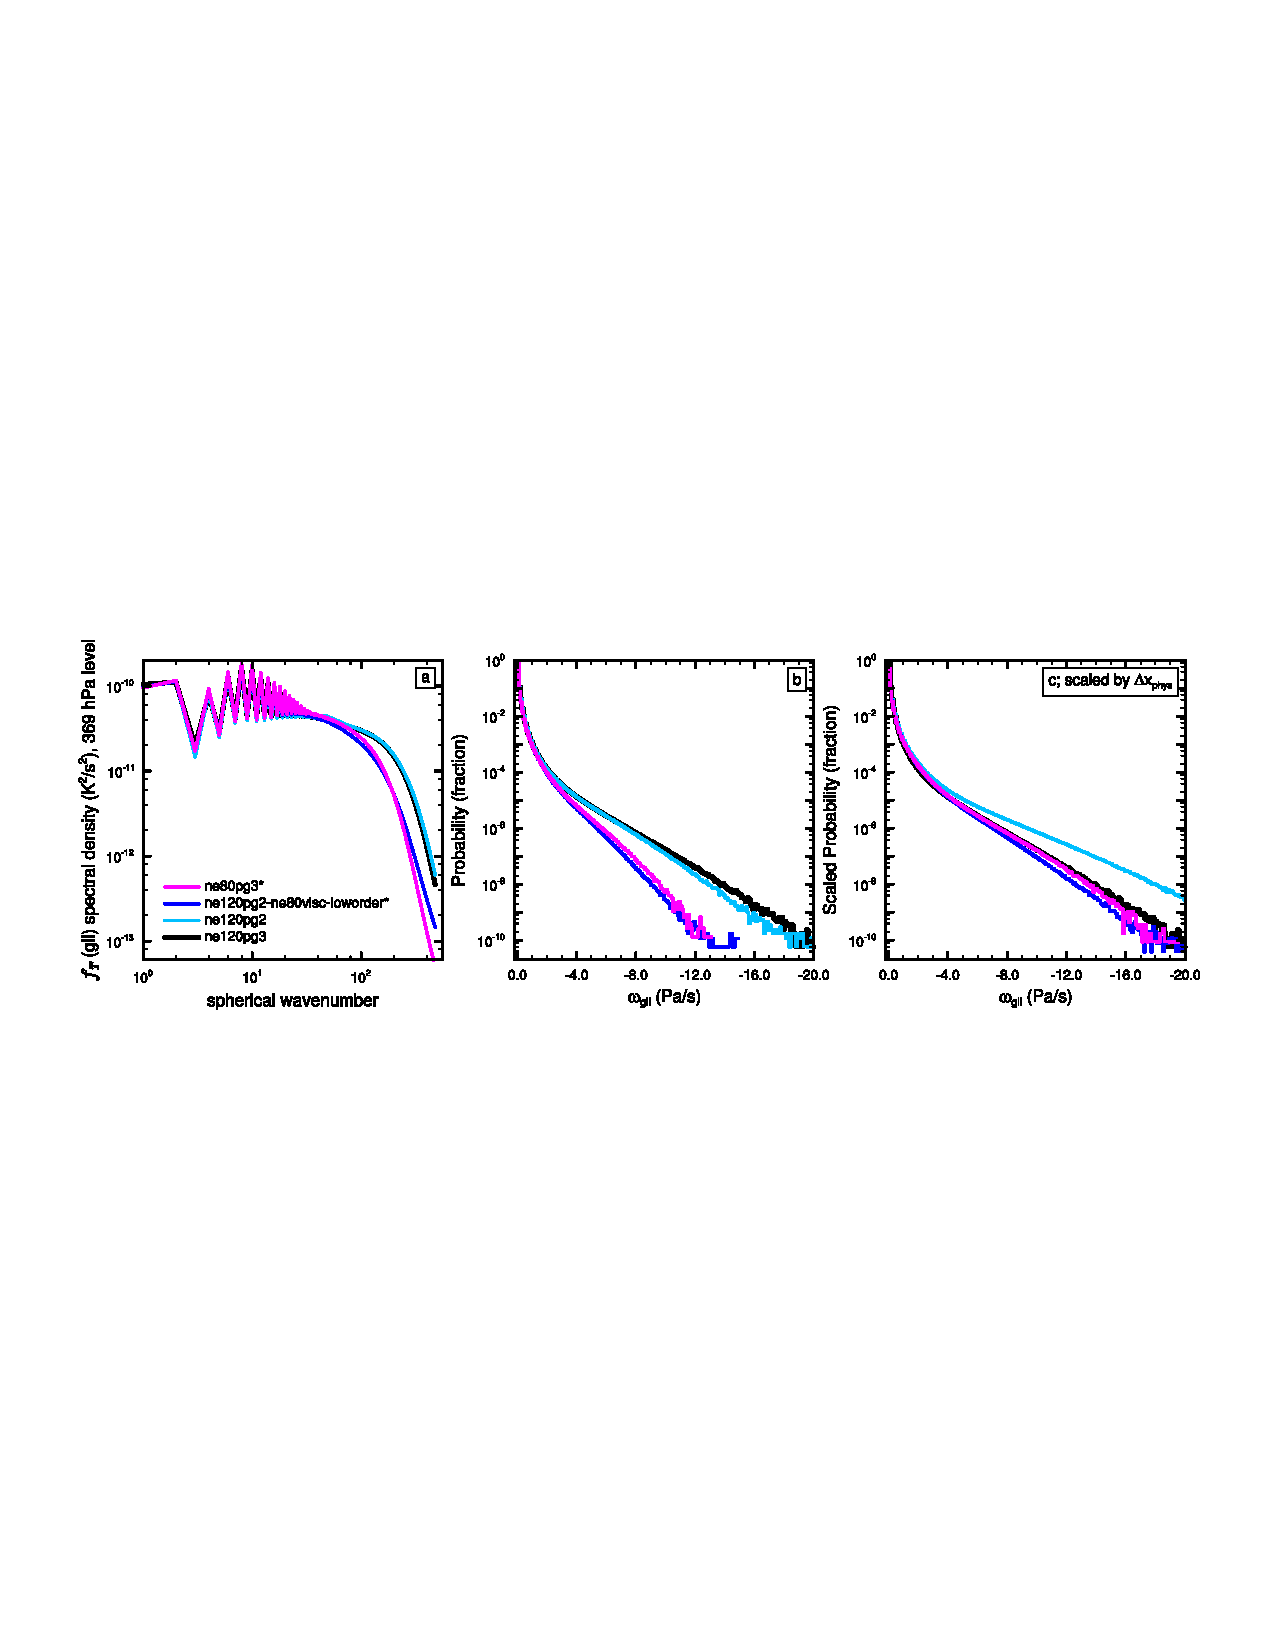
\includegraphics[width=40pc,angle=0]{chapter5/panel_ne80pg3_ne120pg2_ne120pg3.pdf}\\
\end{center}
\caption{As in Figure~\ref{fig:pgXpanel-lores}, but for the high resolution simulations. Asterisks indicate that $\Delta t_{phys}=675 s$, which is larger than that used for the default $ne120$ runs (see Table \ref{table:grids-hi}).}
\label{fig:pgXpanel-hires}
\end{figure}

Figure~\ref{fig:pgXpanel-hires} is the same as Figure~\ref{fig:pgXpanel-lores}, but for the high resolution simulations. While the $ne80pg3$ forcing spectra begins to drop off near wavenumber 100, the $ne120pg2$ and $ne120pg3$ drop off closer to wavenumber 200, and their spectra lie on top of one another (Figure~\ref{fig:pgXpanel-hires}a). The PDF's of (upward) $\omega^{(gll)}$ show that the $ne120$ distributions lie on top of one another, and while not a perfect match, both $ne120$ runs have substantially more frequent large magnitude vertical motion than in the $ne80pg3$ run (Figure~\ref{fig:pgXpanel-hires}b). As in the low resolution runs, the similarity of the $ne120$ forcing spectra and $\omega^{(gll)}$ distributions indicate that the forcing scale of the $ne120pg2$ run is not determined by the physics grid spacing, but rather the dynamics grid spacing. This is also evident from the over-prediction of the frequency of large magnitude $\omega^{(gll)}$ compared with the $ne120pg3$ run, through scaling the $ne120pg2$ PDF and setting the forcing scale proportional to $\Delta x_{phys}$ in equation~\eqref{eq:pdf} (Figure~\ref{fig:pgXpanel-hires}c).

In the $ne120pg2$ simulation, the dynamics grid determines the forcing scale for the same two reasons found in the low resolution runs. The high-order mapping of the physics to the dynamics is important for reconstructing scales not supported on the $pg2$ grid, and scaling the viscosity coefficients by the dynamics grid spacing is also important. But in order to recreate the $ne80pg3$ solution using the $ne120pg2$ grid, the physics time-steps must be the same for these two grids. Combining all three modifications leads to an $ne120pg2$ solution that resembles the $ne80pg3$ run ($ne120pg2-ne80visc-loworder*$ in Figure~\ref{fig:pgXpanel-hires}). The forcing spectrum and distribution of $\omega^{(gll)}$ match that of the $ne80pg3$ run, and scaling the PDF by $\Delta x_{phys}$ closely resembles the $ne120pg3$ distribution.

\paragraph{Across Resolutions}\label{sec:allres} ~\\

 \begin{table}
 \caption{$\Delta x$ and $\Delta t$ for the physics and dynamics in the high resolution simulations. $\Delta x$ is computed as the average equatorial grid spacing.}
 \centering
 \begin{tabular}{llcccc}
 \hline
 Grid name & $\Delta x_{dyn}$  & $\Delta t_{dyn}$ & $\Delta x_{phys}$  & $\Delta t_{phys}$ \\
 \hline
   {\tt{ne}}40{\tt{pg3}}  & 83.4km & 222.5s  & 83.4km & 1350s \\
   {\tt{ne}}60{\tt{pg2}}  & 55.6km & 150s  & 83.4km & 900s \\
   {\tt{ne}}60{\tt{pg3}}  & 55.6km & 150s  & 55.6km & 900s \\
 \hline
 \end{tabular}
 \label{table:grids-med}
 \end{table}
 
Three intermediate resolution aqua-planets are run to provide a continuous representation of the solution spanning from low to high resolution (Table~\ref{table:grids-med}). Figure~\ref{fig:diags} is scatter plot of the climatological global mean state versus $\Delta x_{dyn}$ for all model configurations listed in Tables~\ref{table:grids-lo}$-$\ref{table:grids-med}. The fields plotted in the figure, upward $\omega$, and the two components of precipitation, stratiform precipitation rate (CLUBB) and deep convective precipitation rate (ZM), are all sensitive to resolution. Upward $\omega$ and CLUBB precipitation decreases, and ZM precipitation increases monotonically with $\Delta x_{dyn}$. The $pg2$ solutions have very similar values to the $pg3$ solutions, although they are slightly offset towards the lower resolution side of the plots. The differences between the $pg2$ and $pg3$ solutions are much less then the differences between $pg2$ and configurations where the physics and dynamics grids are both equal to the $pg2$ physics grid resolution (e.g., $ne40pg3$ compared with $ne60pg2$). The mean state of the configurations resembles that of the transients discussed in the previous sections; the coarser $pg2$ physics grid does not appear to degrade the resolved scales of motion, which are primarily determined by the dynamics grid resolution.

\begin{figure}[t]
\begin{center}
\noindent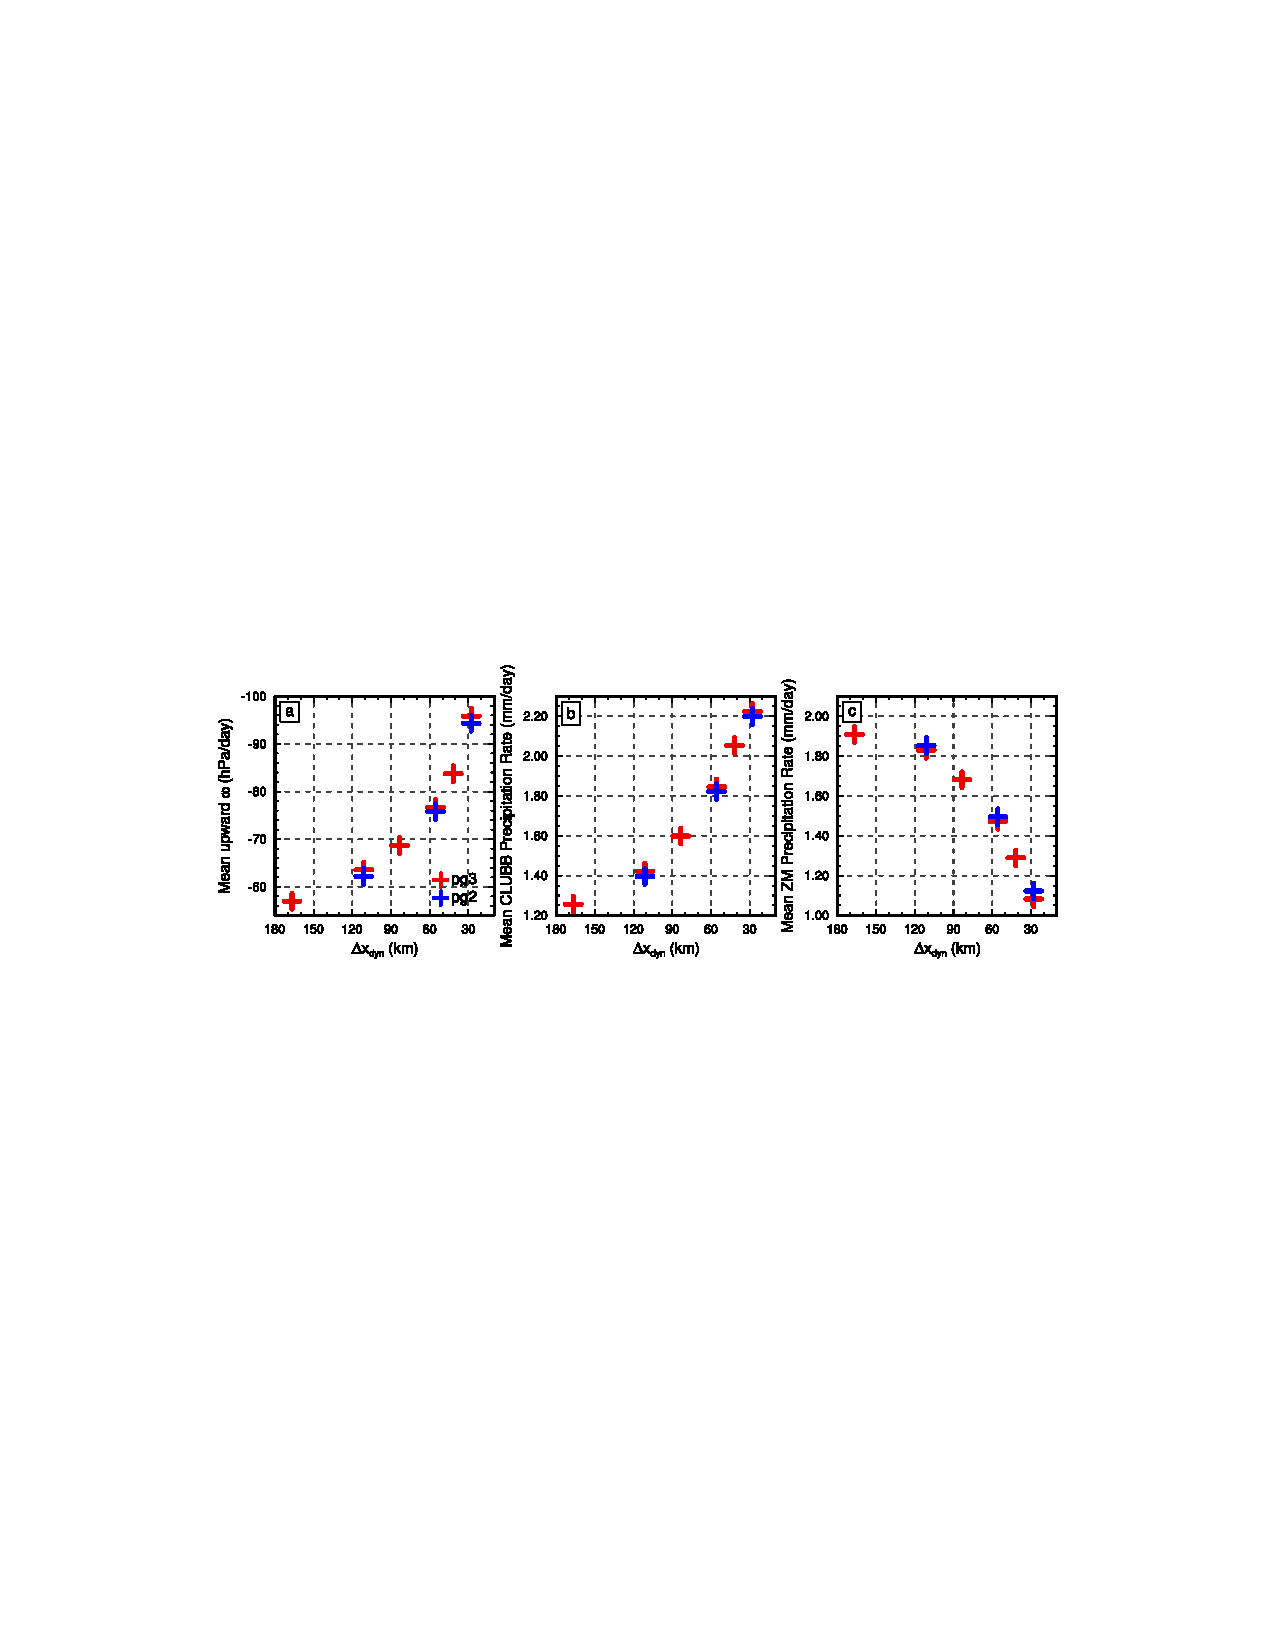
\includegraphics[width=35pc,angle=0]{chapter5/panel_diags.pdf}\\
\end{center}
\caption{Global mean, time-mean (a) upward $\omega$, (b) CLUBB precipitation rate and (c) parameterized deep convective precipitation rate. All means computed from the final 11 months of one-year simulations, and upward $\omega$ is computed using 6-hourly output.}
\label{fig:diags}
\end{figure}

\subsection{Conclusions}\label{sec:conclusions}

This study documents the implementation of a coarser resolution physics grid into the Community Atmosphere Model (CAM), with spectral element dynamics (based on a dry-mass vertical coordinate) and conservative semi-Lagrangian advection of tracers (CAM-SE-CSLAM). The spectral-element and tracer advection grids are mapped to a finite-volume physics grid after \cite{HL2018MWR}, but containing $\frac{2}{3}$ fewer degrees of freedom in each horizontal direction. Mapping from the coarser physics grid to the dynamics and tracer grids is performed with high-order reconstructions, and a tendency mapping algorithm is developed to ensure shape preservation, consistency, linear-correlation preservation and mass conservation. These numerical properties are verified to a high degree of precision through idealized tests.

The coarser resolution physics grid is designed to eliminate grid imprinting that manifests for non-smooth problems using element-based high-order Galerkin methods. The physics grid control volumes encompass a region of the element such that an isotropic representation of the numerics is provided to the physical parameterizations, and it was hypothesized that this method eliminates grid imprinting from the element boundaries. Using a Held-Suarez configuration modified with real-world topography, it was shown that element boundary noise over steep topography is eliminated from the coarser physics grid solution, consistent with our hypothesis.

Physical parameterizations make up a significant fraction of the total computational cost of atmosphere models, and the coarser physics grid may be used to reduce this overhead. The cost savings is due to the factor $\frac{4}{9}$ fewer grid columns in which the physics need be computed, and for CESM2.1, where CAM6 physics makes up about half the cost of the overall model \citep{LetAl2018JAMES}, corresponds to a potential $25\%$ fewer core hours. The authors sought to understand whether the reduction in computational cost occurs at the expense of a degraded solution, through aliasing the dynamics to the coarser resolution physics. An exhaustive number of grids were developed and run in an aqua-planet configuration, and confirm that the resolved scales of motion are not degraded through the use of a coarser resolution physics grid. It was found that the resolved scales are primarily determined by the effective resolution of the dynamical core. This was attributed to two factors; (1), explicit numerical dissipation by the dynamics blurs the distinction between solutions on the physics, dynamics or tracer grids, and (2), that high-order mapping of the physics tendencies to the dynamics and tracer grids reconstructs scales that are not supported on the coarser physics grid.

The coarser physics grid in CAM-SE-CSLAM provides significant cost savings with little to no downside. The coarser physics grid replicates solutions from the conventional method of evaluating the physics at the same resolution as the dynamical core, removes grid imprinting from the solution and runs efficiently on massively parallel systems. The coarser physics grid may be leveraged to reduce the computational burden as a component of increasingly expensive Earth System Models, or permit once unattainable throughputs for high-resolution climate simulations. The coarser physics grid configuration of CAM-SE-CSLAM is well positioned to address the scientific challenges ahead, as a formidable next generation climate model.
 \label{sec:chapter5}

\newpage
\begin{center}
\section{Parameterized convection, grid-scale clouds and resolution sensitivity in CAM-SE-CSLAM}
%\chapter{\bf{\normalsize Parameterized convection, grid-scale clouds and resolution sensitivity in CAM-SE-CSLAM}}
\end{center}
%\addcontentsline{toc}{section}{\protect\numberline{}Parameterized convection, grid-scale clouds and resolution sensitivity in CAM-SE-CSLAM}
%\addcontentsline{toc}{chapter}{\protect\numberline{}Parameterized convection, grid-scale clouds and resolution sensitivity in CAM-SE-CSLAM}
\subsection{Introduction}

An increasing number of atmospheric dynamical cores are being developed to maximize efficiency on massively parallel systems, paving the way towards regionally high-resolution ($\Delta x = 50$ km or less), or even globally high resolution simulations \citep{Z2014QJRMS,HETAL2016JCLIM,DCMIP16,LetAl2018JAMES}. Incorporating these advances into Atmospheric General Circulation Models (AGCMs) requires the development of physical parameterizations appropriate for the diversity of grid configurations that dynamical cores are now able to support, referred to as scale-aware physics. The most common approach to understand and develop scale-aware physics has been through the lens of limited area, cloud resolving simulations \citep{PC2008JAS,AW2013JAS,SZ2018JCLIM}. In filtering cloud resolving solutions to some target, lower resolution resembling an AGCM grid, and studying how the filtered moments vary as a function of target grid resolution, one may develop a more general relationship between resolved and unresolved scales. While this approach is likely necessary for developing scale-aware physics, it is not sufficient. The equations of motions of motion have inherent scale dependencies \citep{O1981JAS,WETAL1997MWR,PG2006JAS,J2017JAMES}, and the resolved dynamics act accordingly to the scales a grid is able to support. Scale-aware physics should also accommodate these dependencies.

The sensitivity of the Community Atmosphere Model (CAM) to horizontal resolution is well documented over the last few decades \citep{KW1991JGR,WETAL1995CD,W1999T,W2008TELLUS,LETAL2011TELLUS,RJ2011MWR,RETAL2012ASL,OETAL2013JCLIM,RETAL2013JCLIM,ZetAl2014JCb,LETAL2015JCLIM}. The general tendency is for the atmosphere to become drier and less cloudy, the deep convection scheme less active and the magnitude of resolved vertical motion greater with increasing resolution. \cite{HR2017JCLIM,HR2018JAMES} analyzed a set of CAM simulations and found that resolved updrafts dominate the vertical velocity field of tropical convecting systems at resolutions typical of present day global models ($208.5 km \geq \Delta x \geq 27.8 km$). The scale of resolved updrafts are collocated in the horizontal with the buoyancy produced by grid-scale clouds (also referred to as stratiform clouds in the literature), and are grid limited, conforming to the effective resolution of the model ($5-10\Delta x$). Assuming that there is a characteristic buoyancy length scale associated with a grid resolution, and it is proportional to $\Delta x$, the ratio of the vertical velocity scale of that grid resolution $W$ to a high-resolution reference simulation $W_{ref}$ is:
\begin{equation}
\alpha = \frac{W}{W_{ref}} = \frac{\Delta x_{ref}}{\Delta x} , \label{eq:eq6-1}
\end{equation}
where $\Delta x_{ref}$ is the grid-spacing of a high-resolution reference, and it is assumed that the magnitude and height scale of the buoyancy is unchanged or compensating across resolutions. The physical interpretation of equation~\ref{eq:eq6-1} is a rising column of buoyancy creates a low pressure perturbation of similar horizontal scale in its wake, and this pressure gradient scales like $\Delta x^{-1}$, facilitating convergence into the pressure minimum and the resultant vertical velocity also scales like $\Delta x^{-1}$. While \cite{HR2017JCLIM} found that equation~\ref{eq:eq6-1} over-predicted the change in vertical velocity across resolutions in their aqua-planet simulations, \cite{HR2017JCLIM} discovered that this over-prediction was at least in-part, due to time-truncation errors arising from too small a physics time-step, $\Delta t_{phys}$, in the higher resolution simulations.

In this study, it is shown that through scaling $\Delta t_{phys}$ in a manner which avoids large time-truncation errors at higher resolutions {Herrington et al., in review), the analytical scaling in equation~\ref{eq:eq6-1} does explain the change in vertical velocities across resolutions in an aqua-planet configuration using CAM. The implications of equation~\ref{eq:eq6-1} are that for a doubling of the resolution, CAM can simulate the same resolved mass flux in half the area. Grid-scale cloud fraction and regions of ascent are then confined to a smaller areas at higher resolutions; the area and magnitude of subsiding motion also increases with resolution. Greater subsiding motion results in a drier and more stable atmosphere, which reduces the frequency the deep convection scheme is triggered. Section $6.2$ describes the model and experimental design, section 6.3 presents results and section 6.3 provides the conclusions.

\subsection{Methods}

\subsection{Results}

The probability density function (PDF) of negative, or upward vertical pressure velocities $\omega$ in the aqua-planets are shown in Figure~\ref{fig:2pdf}a. The magnitude of upward $\omega$ increases in a monotonic way with resolution, with positive, or downward $\omega$ behaving similarly (not shown). The PDF's may be scaled to the high-resolution $ne120$ resolution, through $P(\omega)_s = \alpha P (\omega / \alpha)$, where $\alpha$ is the scale factor equation~\ref{eq:eq6-1}. The scaled PDF's all line up on top of the high-resolution reference (Figure~\ref{fig:2pdf}b); equation~\ref{eq:eq6-1} explains the variation in vertical velocity across resolutions to first order. 

\begin{figure}[t]
\begin{center}
\noindent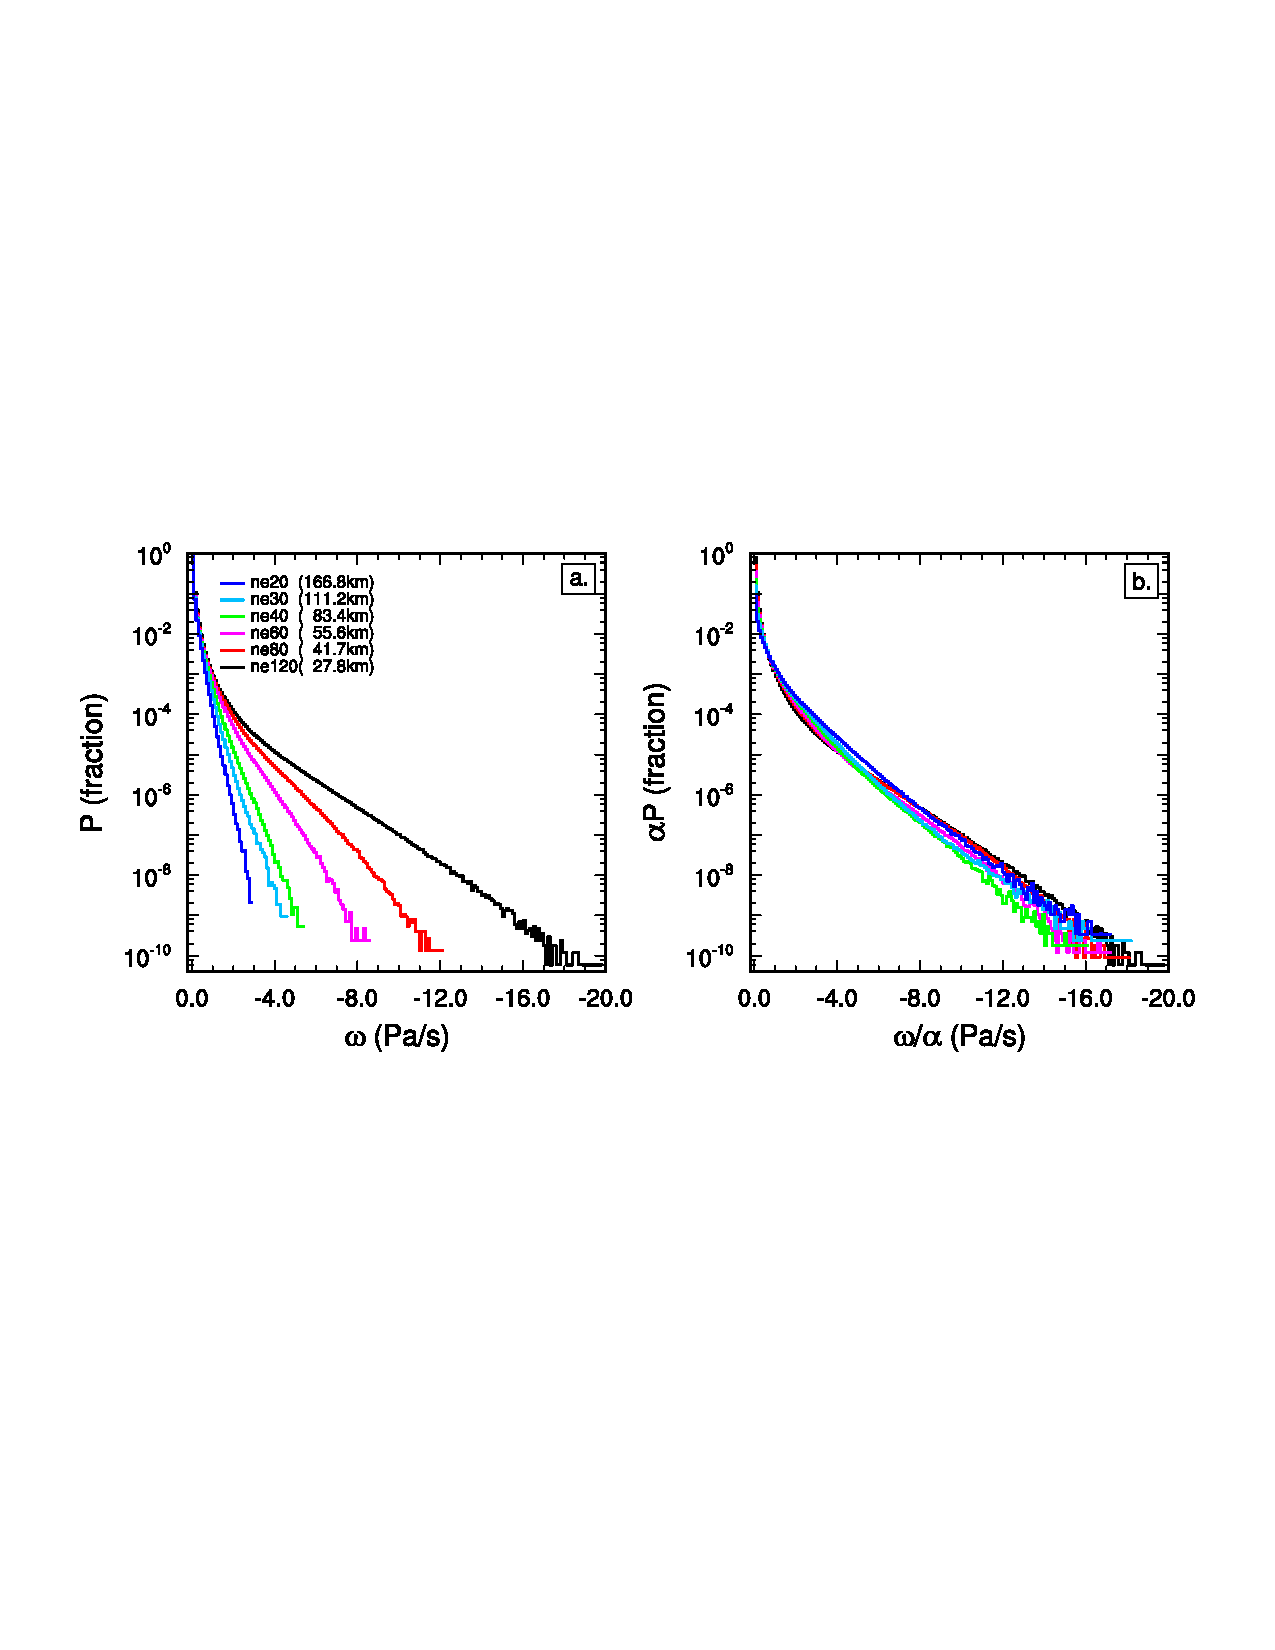
\includegraphics[width=33pc,angle=0]{chapter6/temp_2pdf.pdf}\\
\end{center}
\caption{}
\label{fig:2pdf}
\end{figure}

The impact of the changing vertical velocity field on the global mean state can be understood through decomposing the mass weighted global mean $\omega$ into upward and downward components,
\begin{equation}
\overline{\langle \omega \rangle} = \overline{\langle f_{u} \rangle} \, \overline{\langle \omega_{u} \rangle} + \overline{\langle f_{d} \rangle} \, \overline{\langle \omega_{d} \rangle}, \label{eq:eq6-2}
\end{equation}
where $\langle f_x \rangle$ and $\langle \omega_x \rangle$ refers to the mass weighted fraction and mass weighted mean $\omega$, respectively, subscript $u$ refers to upward motion and $d$, downward motion; the overbars indicate is a time mean global mean. This components of equation~\ref{eq:eq6-2} are shown in Figure~\ref{fig:8panel}a,b,e,f for the six aqua-planet simulations. The magnitude of both $\overline{\langle \omega_{u} \rangle}$ and $\overline{\langle \omega_{d} \rangle}$ increase monotonically with resolution, the upward component increasing more than the downward component. In contrast, $\overline{\langle f_{u} \rangle}$ decreases with resolution while $\overline{\langle f_{d} \rangle}$ increases, although in both cases there is a reversal in this trend in the highest resolution simulation, $ne120$. Note that the magnitude of the change in $\overline{\langle f_{u} \rangle}$ and $\overline{\langle f_{d} \rangle}$ is small, a range of about $0.015$ across all simulations. Figure~\ref{fig:8panel}e,g shows that the products  $\overline{\langle f_{u} \rangle} \, \overline{\langle \omega_{u} \rangle}$ and $\overline{\langle f_{d} \rangle} \, \overline{\langle \omega_{d} \rangle}$ are equal and opposite, which is a requirement of mass conservation in the model and a convenient check of the calculation. Besides the six aqua-planets described in Section 6.2, 23 additional year-long aqua-planet experiments were carried out at various resolutions, with modified parameters in the dynamical core and the physics. The spread in the components of equation~\ref{eq:eq6-2} in the simulations with perturbed parameters is relatively large for $\overline{\langle f_{x} \rangle}$, compared with $\overline{\langle \omega_{x} \rangle}$.

\begin{figure}[t]
\begin{center}
\noindent\includegraphics[width=33pc,angle=0]{chapter6/temp_diags_8panel.pdf}\\
\end{center}
\caption{}
\label{fig:8panel}
\end{figure}

It is common for the activity of deep convection scheme to become less active with increasing resolution in CAM. This is depicted in Figure~\ref{fig:8panel}d, which shows the global mean fraction of total precipitation arising from the deep convective scheme ({\em{ZM scheme}}) decreasing from about $0.60$ at low resolution ($ne20$) to about $0.32$ at high resolution ($ne120$). The global mean space time fraction the ZM scheme is triggered (hereafter referred to as FREQZM) is highly negatively correlated with $\overline{\langle f_{d} \rangle} \, \overline{\langle \omega_{d} \rangle}$ in the 29 simulations (Pearson's R-value = 0.99; Figure~\ref{fig:8panel}h), more then with any individual component of equation~\ref{eq:eq6-2}. 

Figure~\ref{fig:vomg} shows how these highly correlated quantities, the time mean $\langle f_{d} \rangle \langle \omega_{d} \rangle$ and FREQZM, look in the zonal mean. The ZM scheme is most active in the deep tropics, equatorward of about $10^{\circ}$, decreasing sharply poleward throughout the subtropics and mid-latitudes, and increasing again at high latitudes ($\geq 60^{\circ}$). $\langle f_{d} \rangle \langle \omega_{d} \rangle$ is smallest in the deep tropics (equatorward of about $10^{\circ}$), increasing sharply poleward, throughout the subtropics and then decreasing in the middle latitudes ($40^{\circ}$) and throughout polar regions. FREQZM largely mirrors that pattern, with more frequent activity where $\langle f_{d} \rangle \langle \omega_{d} \rangle$ is small. The correspondence between these two quantities with resolution do not appear to have a zonal structure; $\langle f_{d} \rangle \langle \omega_{d} \rangle$  increases and FREQZM decreases everywhere in proportion with one another across resolutions.

\begin{figure}[t]
\begin{center}
\noindent\includegraphics[width=17pc,angle=0]{chapter6/temp_zonal_fracd*vomgd.pdf}\\
\end{center}
\caption{}
\label{fig:vomg}
\end{figure}

The ZM trigger uses a dilute form of CAPE, and is consistent with the negative relation between $\overline{\langle f_{d} \rangle} \, \overline{\langle \omega_{d} \rangle}$ and FREQZM in the zonal mean, and across resolutions. In the classical, non-dilute case, CAPE can be broken into two main components \citep{Z2002JGR}; instability due to the thermodynamic state of parcels in the boundary layer and the instability generated through advection of dry static energy and moisture by the environment, i.e., the resolved flow. The latter term generally contributes positively to CAPE in regions of ascent and negatively in regions of subsidence, which is consistent with Figure~\ref{fig:vomg}.

\begin{figure}[t]
\begin{center}
\noindent\includegraphics[width=25pc,angle=0]{chapter6/temp_cape.pdf}\\
\end{center}
\caption{}
\label{fig:vomg}
\end{figure}

To further support the supposed negative relation between subsiding motion and CAPE, temperature and moisture profiles are collected from the deep tropics of the simulations, and conditionally sampled depending on whether $\langle \omega \rangle$ is positive or negative, indicating predominantly subsiding or ascending grid columns. The mean temperature and moisture profiles of subsiding and ascending regions are then used to compute the dilute-CAPE used by the ZM scheme, offline. Figure~\ref{fig:cape}b indicates that regions ascent are associated with high value of CAPE in the mean ($>170$ J/kg), and low values in subsiding regions ($>110$ J/kg), due to an anomolous warming layer in the $600-800$ hPa layer, and anomalous moisture deficit throughout the entire column, relative to the mean (not shown). Figure~\ref{fig:cape}a shows that fractional area of air columns in the deep tropics that are subsiding (ascending) changes drastically with resolution, from $0.3$ ($0.7$) in the $ne20$ run, and monotonically increasing (decreasing) with resolution to $0.7$ ($0.3$) in the $ne120$ run. Interestingly, the sum of the product of the fractional areas with their corresponding CAPE values (grey crosses in Figure~\ref{fig:cape}b) gives approximately the same value as the CAPE value resulting from the mean temperature and moisture profiles over the entire deep tropics. The CAPE values in the deep tropics are decreasing with resolution because a larger fraction subsiding columns make up a larger portion of the region with resolution.

\begin{figure}[t]
\begin{center}
\noindent\includegraphics[width=14pc,angle=0]{chapter6/temp_zonal_4reg_dwn.pdf}\\
\end{center}
\caption{}
\label{fig:4reg}
\end{figure}

To further understand how the relationship manifests within the simulations themselves, a logistic regression is performed for each grid column in the simulations. Logistic regression uses an iterative method to fit a continuous variable predictor, $x$ to a binary predictand $p$ \citep{},
\begin{equation}
p = \frac{exp{[b_0 + b_1 x]}}{1 + exp{[b_0 + b_1 x]}}, \label{eq:eq6-3}
\end{equation}
where $b_0$ and $b_1$ are the shape parameters of the exponential. The predictor is chosen as the instantaneous $\langle f_{d} \rangle \langle \omega_{d} \rangle$ of a grid column, and the predictand is whether or not the ZM scheme is active, $1$ for yes and $0$ for no. Since the aqua-planets have zonally symmetric boundary conditions, there is a zonally varying structure in the goodness of fit (R-value) and parameter $b_1$ (hereafter referred to as the sensitivity parameter). Figure~\ref{fig:4reg}a,b, shows the zonal mean R-values and sensitivity parameter, which indicates the goodness of fit is greatest in the deep tropics. Figure~\ref{fig:4reg}d shows the time mean zonal mean latent heat flux in the simulations, which is expected to increase CAPE through the component associated with the thermodynamic state of boundary layer parcels. In the deep tropics, the latent heat flux is small, and the sensitivity parameter is large and negative, indicating that subsiding motion is successfully depressing CAPE, and the activity of the ZM scheme.

Poleward of $10^{\circ}$, the R-value decreases to a local minimum between $10^{\circ} - 15^{\circ}$ latitude, and the magnitude of the sensitivity parameter steeply declines. Even though the subsiding motion is increasing polewards of $10^{circ}$, this motion is less effective in depressing the convection scheme. The local minimum in the R-value corresponds with a local maximum in the latent heat fluxes, indicating that the ZM scheme is primarily responding to the instability of the boundary layer due to large surface latent heat fluxes. The CAPE values in this region ($10^{\circ} - 15^{\circ}$) latitude are likely to be small, since ZM precipitation rate consists of mostly drizzle (Figure~\ref{fig:4reg}c). It is likely the preponderance of drizzle in this region is a result of the largely subsiding motion (Figure~\ref{fig:vomg}) constraining CAPE form becoming too large. AGCMs are known to suffer from an excess drizzle bias \citep{} in this approximate region, and this analysis indicates that the drizzle bias is in CAM is due to the use of a CAPE closure in the ZM scheme.   

\subsection{Conclusions} \label{sec:chapter6}

\newpage
\begin{center}
\section{Conclusions}
%\chapter{\bf{\normalsize Conclusions}}
\end{center}
%\addcontentsline{toc}{section}{\protect\numberline{}Conclusions}
%\addcontentsline{toc}{chapter}{\protect\numberline{}Conclusions}
The requirement that Atmospheric General Circulation Models (AGCMs) exhibit convergent solutions with increasing horizontal resolution was not historically pursued by the community, and as a result many AGCM solutions, such as NCAR's Community Atmosphere Model (CAM), change drastically with resolution. Convergent solutions were likely not pursued during the early AGCM development phase (1950s through the 1980s) due to computational limitations. 

The expanse of computing power beginning around the 1990s permitted convergence tests that indicated AGCMs have weak convergence properties. This issue had largely been ignored, or at least had not become a priority to model developers until recently. Dynamical cores are now more commonly developed with unstructured meshes, which allows for substantial grid flexibility and brining to forefront the issue of convergence. The pursuit of {\em{scale-aware physics}} is in essence an effort to develop closures that result in AGCM solutions to converging with increasing resolution, and that those solutions converge to some reasonable depiction of the atmosphere we live in.

\subsection{Summary}

This work is an effort to understand the specific reasons CAM produces very different solutions with increasing horizontal resolution ---which components of the model are responding to a change in resolution, why is it sensitive to resolution and how does it feedback onto other model components. CAM is an extremely complex model. Understanding why CAM simulates a certain feature a certain way is by no mean trivial. Issac Held authored a paper in 2005 titled {\em{The Gap between Simulation and Understanding in Climate Modeling}} \citep{H2005BAMS}, advocating for the community to shift focus more towards understanding these models. He suggests using a hierarchy of models, from the simplest to the most complex, in order to truly nail down the underlying causes of a phenomenon in an AGCM. This is the approach taken in this thesis.

Chapter~\ref{sec:chapter2} presents the sensitivity of the mean state of CAM, version 4 to horizontal resolutions typical of present-day AGCMs in an aqua-planet configuration. Weak convergence of the mean state is characterized by a progressive drying of the atmosphere and large reductions in cloud coverage with increasing resolution. Analyses of energy and moisture budgets indicate that these trends are balanced by variations in moisture transport by the resolved circulation, and a reduction in activity of the convection scheme. In contrast, the large-scale precipitation rate increases with resolution, which is approximately balanced by greater advection of dry static energy associated with more active resolved vertical motion in the ascent region of the Hadley cell.

An explanation for the sensitivity of the mean state to horizontal resolution is proposed, based on linear Boussinesq theory. The authors hypothesize that an increase in horizontal resolution in the model leads to a reduction in horizontal scale of the diabatic forcing arising from the column physics, facilitating finescale flow and faster resolved convective updrafts within the dynamical core, and steering the coupled system toward a new mean state. This hypothesis attempts to explain the underlying mechanism driving the variations in moisture transport observed in the simulations.

In Chapter~\ref{sec:chapter3}, a set of idealized experiments are developed in CAM to understand the vertical velocity response to reductions in forcing scale that occurs when the horizontal resolution is increased. The test consists of a set of rising bubble experiments, in which the horizontal radius of the bubble and the model grid spacing are simultaneously reduced. The test is performed with moisture, through incorporating moist physics routines of varying complexity, although convection schemes are not considered. Results confirm that the vertical velocity in CAM is to first-order, proportional to the inverse of the horizontal forcing scale, which is consistent with a scale analysis of the dry equations of motion. In contrast, experiments in which the physics time step $\Delta t_{phys}$ are relaxed back to more conventional values results in severely damped vertical motion at high resolution, degrading the scaling. A set of aqua-planet simulations using different physics time steps are found to be consistent with the results of the idealized experiments.

The following two chapters arose from work performed during a year-long visit at NCAR as an Advanced Study Program(ASP) graduate student visitor. Chapter~\ref{sec:chapter4} contains a detailed analysis of the physics-dynamics coupling in CAM's spectral-element dynamical core (CAM-SE), which is uses a continuous Galerkin method, and introduces a new coupling approach. Atmospheric modeling with element-based high-order Galerkin methods presents a unique challenge to the conventional physics-dynamics coupling paradigm, due to the highly irregular distribution of nodes within an element and the distinct numerical characteristics of the Galerkin method. The conventional coupling procedure is to evaluate the physical parameterizations ({\em{physics}}) on the dynamical core grid. Evaluating the physics at the nodal points exacerbates numerical noise from the Galerkin method, enabling and amplifying local extrema at element boundaries. 

Grid imprinting may be substantially reduced through the introduction of an entirely separate, approximately isotropic finite-volume grid for evaluating the physics forcing. Integration of the spectral basis over the control-volumes provides an area average state to the physics, which is more representative of the state in the vicinity of the nodal points rather than the nodal point itself, and is more consistent with the notion of a ``large-scale state'' required by conventional physics packages. This study documents the implementation of a quasi-equal area physics grid into CAM-SE, and is shown to be effective at mitigating grid imprinting in the solution. The physics grid is also appropriate for coupling to other components within the Community Earth System Model, since the coupler requires component fluxes to be defined on a finite-volume grid, and one can be certain that the fluxes on the physics grid are indeed, volume-averaged.

Chapter~\ref{sec:chapter5} describes the implementation of a coarser resolution physics grid into CAM-SE. The dry dynamics is represented by the spectral element dynamical core and tracer transport is computed using the Conservative Semi-Lagrangian Finite Volume Method (CAM-SE-CSLAM). Algorithms are presented that map fields between the dynamics and physics grids while maintaining numerical properties ideal for atmospheric simulations such as mass conservation and mixing ratio shape and linear-correlation preservation. The results of experiments using the lower resolution physics grid are compared to the conventional method in which the physics and dynamical grids coincide. The lower resolution physics grid consists of control volumes designed to provide an isotropic representation of the dynamics to the physical parameterizations, and eliminates grid imprinting, even in regions with steep topography. 

The impact of the coarser resolution physics grid on the resolved scales of motion is analyzed in an aqua-planet configuration, across a range of dynamical core grid resolutions. Through analyzing the relationship between the physics forcing and resolved vertical motion, it was determined that the effective resolution of the model is not degraded through the use of a coarser resolution physics grid. Since the physics makes up about half the computational cost of the conventional CAM-SE-CSLAM configuration, the coarser physics grid may allow for significant cost savings with little to no downside.

Chapter~\ref{sec:chapter6} is the final chapter, and puts together a full picture on the causes of resolutions sensitivity in aqua-planets via a thorough analysis of the CAM-SE-CSLAM simulations from Chapter~\ref{sec:chapter5}. Through scaling the $\Delta t_{phys}$ in the aqua-planets such that the large time-truncation errors discovered in Chapter~\ref{sec:chapter3} may be avoided, it was found that the vertical velocity field everywhere in the model is indeed inversely proportional to the grid spacing of the model. The scaling arises because grid-scale clouds are grid limited; their horizontal extent is set by the effective resolution of the model. The dynamics reacts to grid limited clouds through pressure perturbations of the same scale, and so the pressure gradients, and likewise the vertical velocity both scale in proportion to the inverse of the grid spacing. The scaling indicates that for a doubling of the resolution, the resolved mass flux may be achieved in half the area, which then confines the ascending regions to smaller regions of the model with increasing resolution. To conserve mass, subsiding motion both becomes faster and encompass a larger region in the model with increasing resolution, particularly in the Tropics, which creates a more stable and drier mean state. The tendency towards atmospheric stability with increasing resolution reduces the frequency the deep convection scheme is triggered, and convective precipitation becomes a smaller fraction of the total precipitation rate.

\subsection{Significance and future work}

A solid understanding of the causes of resolution sensitivity in an AGCM is useful in many regards. Many AGCMs now support flexible grid structures, such as variable-resolution grids (VR). VR grids are attractive since they can resolve regional climate processes in a global model, but resolution sensitivity may degrade their value since solutions may be permitted to diverge across the refinement region. To be clear, their are many successful VR studies that do not suffer from the convergence issue, and it is generally safe to use refinement over higher-latitude regions due to relatively subdued buoyancy induced vertical velocities, compared to the tropics. But to completely reconcile this deficiency requires the development of scale-aware physics. Scale-aware physics should be built in part, to anticipate and correct the sensitivity of AGCMs to horizontal resolution, which of course, requires knowledge of the causes of resolution sensitivity.

\begin{figure}[t]
\begin{center}
\noindent\includegraphics[width=33pc,angle=0]{chapter7/asp_panel.png}\\
\end{center}
\caption{(a.) Variable resolution grid proposed for the pre-industrial control; grid lines delineate the element boundaries of the spectral-element dynamical core, corresponding to an approximate grid spacing of 111.2km in the coarse region and 27.8km in the refined region. CAM-SE $F$ compset simulations using (b.) a uniform 111.2km grid and (c.),(d.) CAM-VR \citep{VETAL2018TC}. Shown are the climatological (1980-1999) (b.),(c.) annually accumulated precipitation difference (mm w.e.) and (d.) JJA 2-meter air temperature difference (K) from the RACMO2 regional climate model simulation.}
\label{fig:se-mesh}
\end{figure}

CAM-SE supports variable resolution grids (CAM-VR), and due to the vast modeling experience that came of this thesis, I was able to assist in a CAM-VR study with regional grid refinement over the big ice sheet in Greenland \citep[Figure~\ref{fig:se-mesh}a;][]{VETAL2018TC}. Recent attempts to couple NCAR's ice sheet model to CAM results in unrealistic ice sheet expansion of the Greenland Ice Sheet due to a high-precipitation bias in southern Greenland, and a summer cold bias on the coastal margins (W. Lipscomb, personal communication). Using CAM-VR, the precipitation bias is successfully improved (Figures~\ref{fig:se-mesh}b,c), indicating the usefulness of the VR approach. Unfortunately, the summer temperature bias remains (Figure~\ref{fig:se-mesh}d). The author has plans to understand and reconcile this bias as an ASP Postdoctoral at NCAR, which would alleviate a major obstacle to realistic simulations of the Greenland Ice Sheet. \label{sec:chapter7}

\newpage
\section{APPENDICES}
%\chapter*{\bf{\normalsize APPENDICES}}
%\addcontentsline{toc}{section}{\protect\numberline{}APPENDICES}
%\addcontentsline{toc}{chapter}{\protect\numberline{}APPENDICES}
%%%%%%%%%%%%%%%%%%%%%%%%%%%%%%%%%%%%%%%%%%%%%%%%%%%%%%%%%%%%%%%%%%%%%
% APPENDIXES
%%%%%%%%%%%%%%%%%%%%%%%%%%%%%%%%%%%%%%%%%%%%%%%%%%%%%%%%%%%%%%%%%%%%%
%
% Use \appendix if there is only one appendix.
\appendix
The mapping of the physics tendencies from the physics grid to the GLL grid is done with tensor-cubic Lagrange interpolation. The elements of the cubed-sphere in SE are created from an equi-angular gnomonic projection. Consider one element $(\alpha,\beta) \in \left[ \alpha^{(elem)}_1,\alpha^{(elem)}_2 \right]\times \left[ \beta^{(elem)}_1,\beta^{(elem)}_2\right]$, where $(\alpha,\beta)$ are central angle coordinates and $\alpha^{(elem)}_1$ and $\alpha^{(elem)}_2$ are the minimum and maximum central angles in the $\alpha$-coordinate direction, respectively, and similarly for $\beta$. Let $\Delta \alpha^{(elem)}=\alpha^{(elem)}_2-\alpha^{(elem)}_1$ and $\Delta \beta^{(elem)}=\beta^{(elem)}_2-\beta^{(elem)}_1$. The physics grid cell central angle centers are located at
\begin{multline}
(\alpha^{(pg)}_i,\beta^{(pg)}_j)= \Big[ \alpha^{(elem)}_1+\left(i-\tfrac{1}{2}\right) \Delta \alpha^{(pg)},\\
                                      \beta^{(elem)}_1+\left(j-\tfrac{1}{2}\right) \Delta \beta^{(pg)}\Big],
\end{multline}
where $\Delta \alpha^{(pg)}=\Delta \beta^{(pg)}=\frac{\Delta \alpha^{(elem)}}{pg}=\frac{\Delta \beta^{(elem)}}{pg}$. The interpolation is performed in central-angle coordinates using tensor product cubic interpolation. For elements located on a cubed-sphere edge or corner the coordinate system for neighboring elements may be on a different panel. To take into account this coordinate change the central angle locations of physics grid cell centers located on other panels are transformed to the coordinate system of the panel the element in question is located on \cite[the transformations are given in, e.g.,  ][]{NTL2005MWRb}. An illustration is given in Figure \ref{fig:mapping} for an element located in the lower left corner of a panel. The element in question is $(\xi,\chi)\in (-1,1)^2$ where, for simplicity, we have transformed the element coordinates into normalized coordinates $(\xi,\chi) = \left( \frac{ 2\left(\alpha^{(pg)}-\alpha^{(elem)}_1\right)}{\Delta \alpha^{(elem)}}-1,\frac{2\left( \beta^{(pg)}-\beta^{(elem)}_1\right)}{\Delta \beta^{(elem)}}-1\right)$; also used internally in the SE dynamical core \citep[see, e.g., section 3.3 in ][]{LetAl2018JAMES}. The GLL points are located at -1,$-1/\sqrt{1}$, $1/\sqrt{5}$, and 1 in each coordinate direction. Near the edges/corners of an element cubic extrapolation is used if the centered stencil expands beyond the panel.

\begin{figure}[t]
\begin{center}
\noindent\includegraphics[width=20pc,angle=0]{chapter4/mapping.pdf}\\
\end{center}
\caption{Schematic of the coordinate system in which the dimensionally split cubic Lagrange interpolation is computed.  The physics grid centers are marked with asterisks and the GLL points, we are interpolating to, with solid filled circles. The element in which the GLL points are located is  bounded by  thick black lines and located in the lower left corner of a panel. The stippled lines mark the boundaries of the remaining elements. For simplicity we are using the normalized coordinate centered at the element on which the GLL points we are interpolating to are located. Note that the coordinates for points on neighboring panels (using a different local coordinate system) must be transformed to the coordinate system of the element in question.}
\label{fig:mapping}
\end{figure}

\subsection{Defining $\Delta t_{phys}$ across resolutions}\label{sec:app1}
 \cite{HR2018JAMES} developed a moist bubble test, which indicate that time-truncation errors are large at high resolution (about $50km$ or less) using more conventional values for the physics time-step. The test may be able to provide insight on a reasonable scaling of $\Delta t_{phys}$ across resolutions in more complex configurations. In the test a set of non-rotating simulations are initialized with a warm, super-saturated moist bubble, and the grid spacing and bubble radius are simultaneously reduced by the same factor in each run through varying the planetary radius. The test was designed to mimic the reduction in buoyancy length scales that occur when the model resolution is increased in more complex configurations \citep{HETAL2006JCLIM,HR2018JAMES}. 
 
The moist bubble test is performed with CAM-SE-CSLAM and coupled to the simple condensation routine of \cite{K1969MM} across five different resolutions (pertaining to the $ne30$, $ne40$, $ne60$, $ne80$, and $ne120$ grids). The results are expressed as the minimum $\omega$ throughout each one day simulation, and shown in Figure~\ref{fig:bubble}. Two sets of simulations are performed with both $pg3$ and $pg2$, one with $\Delta t_{phys}$ determined by equation~\eqref{eq:dt-scale}, and an equivalent set of simulations with $\Delta t_{phys} = 1800s$ for all resolutions. 

\begin{figure}[t]
\begin{center}
\noindent\includegraphics[width=20pc,angle=0]{chapter5/bubble_test.pdf}\\
\end{center}
\caption{The magnitude of $\omega$ in the $pg3$ solutions are systematically larger than the $pg2$ solutions, which is primarily a result of the damping effect of integrating the basis functions over a larger control volume.}
\label{fig:bubble}
\end{figure}

With the diameters of the bubbles set proportional to $\Delta x_{dyn}$, \cite{HR2018JAMES} has shown that $\omega$ converges to the scaling of equation~\eqref{eq:w-scale} in the limit of small $\Delta t_{phys}$, where small $\Delta t_{phys}$ refers to the CFL limiting time-step used by the dynamics. Equation~\eqref{eq:w-scale} is overlain as grey lines in Figure~\ref{fig:bubble}, with $ne30$ being the reference resolution. The solutions using $\Delta t_{phys}$ from equation~\eqref{eq:dt-scale} follow the scaling, whereas fixing $\Delta t_{phys} = 1800s$ across resolutions damps the solution relative to the analytical solution, progressively more so at higher resolutions. If $\Delta t_{phys}$ is too large, the solution has non-negligible error, which is avoided through scaling $\Delta t_{phys}$ according to equation~\eqref{eq:dt-scale}.

To get a a handle on whether the test is useful for understanding more realistic configurations, four aqua-planet simulations are performed using the CAM6 physics package. A pair of $ne30pg2$ simulations, one in which $\Delta t_{phys}$ is set to the appropriate value from equation~\eqref{eq:dt-scale} ($1800s$), and another where it is set to the $\Delta t_{phys}$ corresponding to the $ne20$ resolution ($2700s$). Similarly, a pair of $ne120pg2$ simulations are performed, one with $\Delta t_{phys}$ set to the value from equation~\eqref{eq:dt-scale} ($450s$), and one with $\Delta t_{phys}$ set to the $ne80$ value ($675s$). 

\begin{figure}[t]
\begin{center}
\noindent\includegraphics[width=20pc,angle=0]{chapter5/panel_pdf_dtphys.pdf}\\
\end{center}
\caption{Probability density distribution of upward $\omega$ everywhere in the model in the aqua-planets using the $ne30pg2$ grid (Left) and the $ne120pg2$ grid (Right). Figure computed for one year of 6-hourly data. The different colors indicate the physics time-steps used in the runs.}
\label{fig:pdf-dtphys}
\end{figure}

Figure~\ref{fig:pdf-dtphys} shows the PDFs of upward $\omega$ computed from a year of six-hourly data in the simulations. At lower resolution, $\Delta t_{phys}$ has only a very small effect on the solution, near the tale-end of the distributions. At high-resolution, values of $\omega$ less then about $-3 Pa/s$ are more frequent in the small $\Delta t_{phys}$ run, with the discrepancy growing more for larger magnitudes of $\omega$. The progressively larger errors with increasing resolution also manifests in the moist bubble tests, indicating that truncation errors arising from large $\Delta t_{phys}$ do exist in more complex configurations.

\subsection{The impact of high-order mapping to the dynamics grids}\label{sec:app2}

Figure~\ref{fig:loworder}a shows a close-up of the wavenumber power spectrum of the forcing on the $pg$ grid (dotted), where it is computed, and on the $GLL$ grid (solid), where it is has been mapped. In $ne30pg3$, the magnitudes are similar on both grids, except the mapping tends to damp the high wavenumbers of the forcing on the $GLL$ grid (greater than 60), but these scales are primarily below the effective resolution of the model and should not effect the solution. For $ne30pg2$, the magnitude of the forcing is actually greater after mapping to the $GLL$ grid, and more similar to the forcing in the $ne30pg3$ simulations. The high-order mapping can therefore replicate the scales of the physics tendencies that occur in the $pg3$ simulation, even though the physics are evaluated on a coarser $pg2$ grid.

\begin{figure}[t]
\begin{center}
\noindent\includegraphics[width=30pc,angle=0]{chapter5/panel_loworder.pdf}\\
\end{center}
\caption{(Left) Wavenumber-power spectrum of the temperature tendencies from the moist physics, at the 369 hPa level, and (right) probability density distribution of upward $\omega$, everywhere in the model, for three year-long aqua-planet simulations. Solid lines refer to values of on the $GLL$ grids, and dashed lines, the fields on the $pg$ grids. See text for details regarding the three simulations.}
\label{fig:loworder}
\end{figure}

The importance of the high-order mapping can be shown with an additional $ne30pg2$ simulation, using low-order mapping ($ne30pg2-loworder$ in Figure~\ref{fig:loworder}). Specifically, low-order mapping refers to piecewise constant mapping between the $pg2$ and $CSLAM$ grids, and bi-linear mapping from $pg2$ to the $GLL$ grid. The forcing spectrum is now similar on both the $pg2$ and $GLL$ grids, although the low-order mapping tends to damp the forcing on the $GLL$ grid for wavenumbers greater than about 60, scales smaller than the models effective resolution (Figure~\ref{fig:loworder}a). A close up of the PDF of $\omega^{(gll)}$ is provided in Figure~\ref{fig:loworder}b (solid lines). As expected, the frequency of large magnitude $\omega^{(gll)}$ in the low-order run is less compared to the default $ne30pg2$ simulation. 

The dotted lines in Figure~\ref{fig:loworder}b show the PDF of $\omega$ on the $pg$ grids. The frequency of large magnitude $\omega$ is reduced on the $pg$ grids, compared to the state on the $GLL$ grids. This is primarily due to the smoothing effect of integrating the nodal point values over control volumes (H18). The larger $\omega$ values are even less frequent on the $pg2$ grid due to integrating over control volumes $\frac{9}{4}$ times greater than the $pg3$ control volumes. 



\newpage
\section*{REFERENCES}
%\chapter*{\bf{\normalsize REFERENCES}}
\addcontentsline{toc}{section}{\protect\numberline{}REFERENCES}
%\addcontentsline{toc}{chapter}{\protect\numberline{}REFERENCES}
\setlength{\bibsep}{0pt}
{\normalsize
\bibliography{bib}}

\end{document}